%!TEX encoding = UTF-8 Unicode
\documentclass[a4paper]{compendium}
\usepackage[swedish]{babel}
\addto\captionsswedish{%
  \renewcommand{\appendixname}{Appendix}%
}
%TODO: Glossary
%http://tex.stackexchange.com/questions/5821/creating-a-standalone-glossary/5837#5837

\setlength{\columnsep}{16mm}

\title{
{\vspace{-3.0cm}\bf\sffamily\Huge\selectfont  Introduktion till programmering med Scala och Java}
\\ \vspace{1em}%\hspace*{1.5cm}\inputgraphics[width=0.6\textwidth]{../img/gurka} \\
{\sffamily  Kompendium 2: Uppgifter}\\\vspace{2cm}
%
\includegraphics[height=4cm]{../img/scala-logo.png}
%
\includegraphics[height=4cm]{../img/java-logo.png}

\includegraphics[height=12cm]{cover/gurka.jpg}
}

%\author{Redaktör: Björn Regnell}
\date{\raggedbottom%
\vspace{-2em}\begin{minipage}{1.0\textwidth}\centering
EDAA45, Lp1-2, HT 2016\\
Datavetenskap, LTH\\
Lunds Universitet\\
~\\
Kompileringsdatum: \today \\
\url{http://cs.lth.se/pgk}
\end{minipage}
}

\usepackage{multicol}

\usepackage{pgffor}  %% http://stackoverflow.com/questions/2561791/iteration-in-latex
                     %  allows:  \foreach \n in {1,...,4}{ do something with \n }

\usepackage{framed}  %  allows:   \begin{framed}\end{framed}
%\newenvironment{Slide}[2][]
%  {\begin{framed}\setlist{noitemsep}\section*{#2}}
%  {\end{framed}}

\newcommand{\SlideHeading}[1]{} %ignore slide headings
\newcommand{\Subsection}[1]{} %ignore slide sections
\newcommand{\SlideOnly}[1]{} %ignore slide font size

\newif\ifkompendium  % to allow conditional text in slides only showing up in compendium
\kompendiumtrue      % in slides: \kompendiumfalse


%!TEX encoding = UTF-8 Unicode

\newcommand{\ModWeekONE}{Introduktion}
\newcommand{\ExeWeekONE}{expressions}
\newcommand{\LabWeekONE}{kojo}


\newcommand{\ModWeekTWO}{Program, kontrollstrukturer}
\newcommand{\ExeWeekTWO}{programs}
\newcommand{\LabWeekTWO}{--}


\newcommand{\ModWeekTHREE}{Funktioner, abstraktion}
\newcommand{\ExeWeekTHREE}{functions}
\newcommand{\LabWeekTHREE}{irritext}


\newcommand{\ModWeekFOUR}{Objekt, inkapsling}
\newcommand{\ExeWeekFOUR}{objects}
\newcommand{\LabWeekFOUR}{blockmole}


\newcommand{\ModWeekFIVE}{Klasser, datamodellering}
\newcommand{\ExeWeekFIVE}{classes}
\newcommand{\LabWeekFIVE}{--}


\newcommand{\ModWeekSIX}{Mönster, felhantering}
\newcommand{\ExeWeekSIX}{patterns}
\newcommand{\LabWeekSIX}{blockbattle}


\newcommand{\ModWeekSEVEN}{Sekvenser, enumerationer}
\newcommand{\ExeWeekSEVEN}{sequences}
\newcommand{\LabWeekSEVEN}{shuffle}


\newcommand{\ModWeekEIGHT}{Matriser, typparametrar}
\newcommand{\ExeWeekEIGHT}{matrices}
\newcommand{\LabWeekEIGHT}{life}


\newcommand{\ModWeekNINE}{Mängder, tabeller}
\newcommand{\ExeWeekNINE}{lookup}
\newcommand{\LabWeekNINE}{words}


\newcommand{\ModWeekTEN}{Arv, komposition}
\newcommand{\ExeWeekTEN}{inheritance}
\newcommand{\LabWeekTEN}{snake0}


\newcommand{\ModWeekELEVEN}{Kontextuella abstraktioner, api}
\newcommand{\ExeWeekELEVEN}{context}
\newcommand{\LabWeekELEVEN}{snake1}


\newcommand{\ModWeekTWELVE}{Valfri fördjupning, Projekt}
\newcommand{\ExeWeekTWELVE}{extra}
\newcommand{\LabWeekTWELVE}{Projekt0}


\newcommand{\ModWeekTHIRTEEN}{Repetition}
\newcommand{\ExeWeekTHIRTEEN}{examprep}
\newcommand{\LabWeekTHIRTEEN}{Projekt1}


\newcommand{\ModWeekFOURTEEN}{Muntligt prov}
\newcommand{\ExeWeekFOURTEEN}{Munta}
\newcommand{\LabWeekFOURTEEN}{Munta}


\begin{document}

\pagenumbering{roman}

\frontmatter
\maketitle
%!TEX encoding = UTF-8 Unicode
%!TEX root = ../compendium.tex

\clearpage\null\thispagestyle{empty}
\vfill

{
\setlength{\parindent}{0pt}
\emph{Editor}: Björn Regnell \\

%  LIST OF CONTRIBUTORS to https://github.com/lunduniversity/introprog
%    Please contact bjorn.regnell@cs.lth.se if you think you should be
%    on this list, or make a pull request with an update of file briefly
%    describing your contribtion in the commit text.
%    This work is licenced under CC-BY-SA-4.0.
%!TEX encoding = UTF-8 Unicode
%!TEX root = compendium/compendium.tex
\hyphenation{Borg-lund Da-ne-bjer Grampp Palm-qvist Ravn-borg Ro-sen-qvist Schrei-ter Wih-lan-der}
\emph{Contributors} in alphabetical order:
Anders Buhl,
André Philipsson Eriksson,
Anna Axelsson,
Anna Palmqvist Sjövall,
Anton Andersson,
Benjamin Lindberg,
Björn Regnell,
Casper Schreiter,
Cecilia Lindskog,
Dag Hemberg,
Elliot Bräck,
Elsa Cervetti Ogestad,
Emelie Engström,
Emil Wihlander,
Erik Bjäreholt,
Erik Grampp,
Evelyn Beck,
Fredrik Danebjer,
Gustav Cedersjö,
Henrik Olsson,
Hussein Taher,
Jakob Hök,
Jakob Sinclair,
Johan Ravnborg,
Jonas Danebjer,
Jos Rosenqvist,
Maj Stenmark,
Maria Kulesh,
Måns Magnusson,
Nicholas Boyd Isacsson,
Niklas Sandén,
Oliver Persson,
Oscar Sigurdsson,
Oskar Berg,
Oskar Widmark,
Patrik Persson,
Per Holm,
Philip Sadrian,
Sandra Nilsson,
Sebastian Hegardt,
Simon Persson,
Stefan Jonsson,
Theodor Lundqvist,
Tim Borglund,
Tom Postema,
Valthor Halldorsson,
Viktor Claesson,
Wilhelm Wanecek,
William Karlsson.

\\ \newline

\emph{Home}: \url{https://cs.lth.se/pgk} \newline

\emph{Repo}: \url{https://github.com/lunduniversity/introprog} \\ \newline

This compendium is on-going work. \\ \textbf{Contributions are welcome!} \\
\emph{Contact}: \url{bjorn.regnell@cs.lth.se}
\\ \newline

%\emph{Cover art}: Björn Regnell (inspired by Poul Ströyer's illustration of Lennart Hellsing's lyrics to  the childrens song ''Herr Gurka'' with music by Knut Brodin)\\ \newline

~\\ \newline

You can use this work if you respect this \emph{LICENCE}: CC BY-SA 4.0 \\
\url{http://creativecommons.org/licenses/by-sa/4.0/} \\
Please do \emph{not} distribute your solutions to lab assignments and projects.
\\ \newline
Copyright \copyright~ 2015-2017. \\
Dept. of Computer Science, LTH, Lund University. Lund. Sweden.\\
}

%%!TEX encoding = UTF-8 Unicode
%!TEX root = ../compendium.tex

\ChapterUnnum{Framstegsprotokoll} 


\subsubsection*{Genomförda övningar}

\vspace{1em}\noindent 
{Till varje laboration hör en övning med uppgifter som utgör förberedelse inför labben. Du behöver minst behärska grundövningarna för att klara labben inom rimlig tid. Om du känner att du behöver öva mer på grunderna, gör då även extrauppgifterna. Om du vill fördjupa dig, gör fördjupningsuppgifterna som är på mer avancerad nivå. Kryssa för nedan vilka övningar du har gjort, så blir lätt för din handledare att se vilka kunskaper du förvärvat hittills.}

\newcommand{\TickBox}{\raisebox{-.50ex}{\Large$\square$}}
\newcommand{\ExeRow}[1]{\texttt{#1} & \TickBox  &  \TickBox &  \TickBox  \\ \addlinespace }

\begin{table}[h]
\centering
\vspace{2em}
\begin{tabular}{lccc}
\toprule \addlinespace 
{\sffamily\small Övning} & 
{\sffamily\small Grund} &	
{\sffamily\small Extra} &
{\sffamily\small Fördjupning}\\ \addlinespace \midrule \\[-0.7em]
\ExeRow{expressions}
\ExeRow{statements}
\ExeRow{functions}
\ExeRow{data}
\ExeRow{vectors}
\ExeRow{classes}
\ExeRow{traits}
\ExeRow{matching}
\ExeRow{matrices}
\ExeRow{sorting}
\ExeRow{scalajava}
\ExeRow{threads}
\bottomrule
\end{tabular}
\end{table}

\newpage

\subsubsection*{Godkända obligatoriska moment}

\vspace{1em}\noindent 
För att bli godkänd på laborationsuppgifterna och projektuppgiften måste du lösa deluppgifterna och diskutera dina lösningar med en handledare. Denna diskussion är din möjlighet att få feedback på dina lösningar. Ta vara på den!
Se till att handledaren noterar nedan när du blivit godkänd på respektive labb. Spara detta blad tills du fått slutbetyg i kursen. 


\vspace{2.5em}\noindent Namn: \dotfill\\

\vspace{1em}\noindent Namnteckning: \dotfill\\

\newcommand{\LabRow}[1]{\\[-1.1em] \texttt{#1} & \dotfill &  \dotfill  \\ \addlinespace }

\begin{table}[h]
\centering
\vspace{1em}
\begin{tabular}{lcc}
\toprule \addlinespace 
{\sffamily\bfseries\small Lab} & {\sffamily\small Datum gk} &	{\sffamily\small Handledares namnteckning}\\ \addlinespace \midrule \\[-0.5em]
%!TEX encoding = UTF-8 Unicode
%!TEX root = ../compendium2.tex
\LabRow{kojo}
\LabRow{irritext}
\LabRow{blockmole}
\LabRow{blockbattle}
\LabRow{shuffle}
\LabRow{words}
\LabRow{life}
\LabRow{snake}
\LabRow{music}
\LabRow{javatext}
\LabRow{survey}
%\toprule 
\addlinespace \midrule \addlinespace
 \\
{\sffamily\small {\bfseries Projektuppgift} (välj en)	} & \dotfill&\dotfill \\ \addlinespace\addlinespace %\midrule
\texttt{( ) bank}  &  &  \\
\texttt{( ) imageprocessing}  \\
\texttt{( ) tictactoe} \\  
\texttt{( ) }\textit{egendefinerad}  \\
\textit{\small Om egen, ge kort beskrivning:}\\
%\dotfill  \\
\bottomrule
\end{tabular}
\end{table}
%%!TEX root = ../compendium.tex


\ChapterUnnum{Förord} 

Programmering är inte bara ett sätt att ta makten över systemen som styr vårt samhälle. Det är också ett kraftfullt verktyg för tanken. Att lära sig programmering och systemutveckling är första steget på en livslång resa av kontinuerligt lärande. Programmeringsspråk och utvecklingsverktyg kommer och går, men de grundläggande koncepten sekvens, alternativ, repetition och abstraktion som ligger bakom all mjukvara består. 

Detta kompendium utgör kursmaterial för studier i grundläggande programmering, med syfte att ge en solid bas för ingenjörsstudenter och andra som utvecklar system som innehåller mjukvara. 

Kompendiet är framtaget av, med och för studenter och lärare på universitetsnivå, och distribueras som öppen källkod. Det får användas fritt så länge erkännande ges och eventuella ändringar också publiceras som öppen källkod under samma licens som ursprungsmaterialet. På kursens hemsida \href{http://cs.lth.se/pgk}{cs.lth.se/pgk} och repo \href{http://github.com/lunduniversity/introprog}{github.com/lunduniversity/introprog} finns instruktioner om hur du kan bidra till kursmaterialet.

Läromaterialet fokuserar på lärande genom eget arbete och innehåller övningar och laborationer som är organiserade i moduler. Varje modul har ett tema och tillhörande föreläsningsanteckningar.

I kursen används språken Scala och Java för att illustrera grunderna i imperativ och objektorienterad programmering, tillsammans med elementär funktionsprogrammering. Mer avancerad objektorientering och funktionsprogrammering och  lämnas till fortsättningskurser. 



Den kanske viktigaste framgångsfaktorn vid studier i programmering är att bejaka din egen upptäckarglädje och experimentlusta. Det fantastiska med programmering är att dina egna intellektuella konstruktioner faktiskt \emph{gör} något som just \emph{du} har bestämt! Ta vara på det och prova dig fram genom att koda egna idéer -- det är kul när det funkar men minst lika lärorikt är felsökning, buggrättande och alla misslyckade försök som efter hårt arbete vänds till lyckade lösningar och bestående lärdomar. 

Välkommen i programmeringens fascinerande värld och hjärtligt lycka till med dina studier!




\setcounter{tocdepth}{1} % set headings level in table of contents
\tableofcontents
\mainmatter

\pagenumbering{arabic}

%\renewcommand{\SlideHeading}[1]{\subsection{#1}}  %numbering sections in compendium slides

\part{Uppgifter}

\chapter{Introduktion}\label{chapter:W01}
\begin{itemize}[nosep]
\item sekvens
\item alternativ
\item repetition
\item abstraktion
\item programmeringsspråk
\item programmeringsparadigmer
\item editera-kompilera-exekvera
\item datorns delar
\item virtuell maskin
\item värde
\item uttryck
\item variabel
\item typ
\item tilldelning
\item namn
\item val
\item var
\item def
\item if
\item else
\item true
\item false
\item MinValue
\item MaxValue
\item aritmetik
\item slumptal
\item math.random
\item logiska uttryck
\item de Morgans lagar
\item while-sats
\item for-sats
\end{itemize}
%!TEX encoding = UTF-8 Unicode
%!TEX root = ../exercises.tex

\ifPreSolution
\Exercise{\ExeWeekONE}\label{exe:W01}

\begin{Goals}
%!TEX encoding = UTF-8 Unicode

\item Förstå vad som händer när satser exekveras och uttryck evalueras.
\item Förstå sekvens, alternativ och repetition.
\item Känna till literalerna för enkla värden, deras typer och omfång.
\item Kunna deklarera och använda variabler och tilldelning, samt kunna rita bilder av minnessituationen då variablers värden förändras.
\item Förstå skillnaden mellan olika numeriska typer, kunna omvandla mellan dessa och vara medveten om noggrannhetsproblem som kan uppstå.
\item Förstå booleska uttryck och värdena \code{true} och \code{false}, samt kunna förenkla booleska uttryck.
\item Förstå skillnaden mellan heltalsdivision och flyttalsdivision, samt användning av rest vid heltalsdivision.
\item Förstå precedensregler och användning av parenteser i uttryck.
\item Kunna använda \code{if}-satser och \code{if}-uttryck.
\item Kunna använda \code{for}-satser och \code{while}-satser.
\item Kunna använda \code{math.random()} för att generera slumptal i olika intervaller.
\item Kunna beskriva skillnader och likheter mellan en procedur och en funktion.

\end{Goals}

\begin{Preparations}
\item \StudyTheory{01}
\item Du behöver en dator med Scala och Kojo installerad, se appendix~\ref{appendix:compile} och  \ref{appendix:kojo}.
\end{Preparations}

\else

\ExerciseSolution{\ExeWeekONE}

\fi  %%% END \ifPreSolution


\BasicTasks




\WHAT{Para ihop begrepp med beskrivning.}

\QUESTBEGIN

\Task \what

\vspace{1em}\noindent Koppla varje begrepp med den (förenklade) beskrivning som passar bäst:

\begin{ConceptConnections}
  litteral & 1 & & A & kan inträffa medan programmet kör \\ 
  sträng & 2 & & B & att översätta kod till exekverbar form \\ 
  sats & 3 & & C & vid anrop beräknas ett returvärde \\ 
  uttryck & 4 & & D & decimaltal med begränsad noggrannhet \\ 
  funktion & 5 & & E & bra då antalet repetitioner är bestämt i förväg \\ 
  procedur & 6 & & F & en kodrad som gör något; kan särskiljas med semikolon \\ 
  exekveringsfel & 7 & & G & beskriver vad data kan användas till \\ 
  kompileringsfel & 8 & & H & antingen sann eller falsk \\ 
  abstrahera & 9 & & I & för att ändra en variabels värde \\ 
  kompilera & 10 & & J & kombinerar värden och funktioner till ett nytt värde \\ 
  typ & 11 & & K & en sekvens av tecken \\ 
  for-sats & 12 & & L & att införa nya begrepp som förenklar kodningen \\ 
  while-sats & 13 & & M & anger ett specifikt datavärde \\ 
  tilldelning & 14 & & N & kan inträffa innan exekveringen startat \\ 
  flyttal & 15 & & O & bra då antalet repetitioner ej är bestämt i förväg \\ 
  boolesk & 16 & & P & vid anrop sker (sido)effekt; returvärdet är tomt \\ 
\end{ConceptConnections}

\SOLUTION

\TaskSolved \what

\begin{ConceptConnections}
  litteral & 1 & ~~\Large$\leadsto$~~ &  D & anger ett specifikt datavärde \\ 
  sträng & 2 & ~~\Large$\leadsto$~~ &  G & en sekvens av tecken \\ 
  sats & 3 & ~~\Large$\leadsto$~~ &  F & en kodrad som gör något; kan särskiljas med semikolon \\ 
  uttryck & 4 & ~~\Large$\leadsto$~~ &  H & kombinerar värden och funktioner till ett nytt värde \\ 
  funktion & 5 & ~~\Large$\leadsto$~~ &  K & vid anrop beräknas ett returvärde \\ 
  procedur & 6 & ~~\Large$\leadsto$~~ &  J & vid anrop sker (sido)effekt; returvärdet är tomt \\ 
  exekveringsfel & 7 & ~~\Large$\leadsto$~~ &  N & kan inträffa medan programmet kör \\ 
  kompileringsfel & 8 & ~~\Large$\leadsto$~~ &  M & kan inträffa innan exekveringen startat \\ 
  abstrahera & 9 & ~~\Large$\leadsto$~~ &  A & att införa nya begrepp som förenklar kodningen \\ 
  kompilera & 10 & ~~\Large$\leadsto$~~ &  C & att översätta kod till exekverbar form \\ 
  typ & 11 & ~~\Large$\leadsto$~~ &  I & beskriver vad data kan användas till \\ 
  for-sats & 12 & ~~\Large$\leadsto$~~ &  O & bra då antalet repetitioner är bestämt i förväg \\ 
  while-sats & 13 & ~~\Large$\leadsto$~~ &  P & bra då antalet repetitioner ej är bestämt i förväg \\ 
  tilldelning & 14 & ~~\Large$\leadsto$~~ &  L & för att ändra en variabels värde \\ 
  flyttal & 15 & ~~\Large$\leadsto$~~ &  E & decimaltal med begränsad noggrannhet \\ 
  boolesk & 16 & ~~\Large$\leadsto$~~ &  B & antingen sann eller falsk \\ 
\end{ConceptConnections}

\QUESTEND






\WHAT{Utskrift i Scala REPL.}

\QUESTBEGIN

\Task \what

\vspace{1em}\noindent Starta Scala REPL \Eng{Read-Evaluate-Print-Loop}.

\begin{REPLnonum}
> scala
Welcome to Scala 3.0.1 (OpenJDK 64-Bit Server VM, Java 11.0.8).
Type in expressions for evaluation. Or try :help.
scala -version.
scala>
\end{REPLnonum}

\Subtask Skriv efter prompten \code{scala>} en sats som skriver ut en valfri (bruklig/knasig) hälsningsfras, genom anrop av proceduren \code{println} med något strängargument. Tryck på \textit{Enter} så att satsen kompileras och exekveras.

\Subtask Skriv samma sats igen (eller tryck pil-upp) men ''glöm bort'' att skriva högerparentesen efter argumentet innan du trycker på \textit{Enter}. Vad händer?

\begin{framed}
\noindent\emph{Tips inför fortsättningen:} Det finns många användbara kortkommandon och andra trix för att jobba snabbt i REPL. Be gärna någon som kan dessa trix att visa dig hur man kan jobba snabbare. Läs appendix \ref{appendix:compile:REPL} och prova sedan att kopiera och klistra in text. Använd piltangenterna för att bläddra i historiken, Ctrl+A för att komma till början av raden, Ctrl+K för att radera resten av raden, etc.
\end{framed}



\SOLUTION
\TaskSolved \what

\SubtaskSolved Till exempel:
\begin{REPLnonum}
scala> println("hejsan svejsan")
\end{REPLnonum}

\SubtaskSolved Om högerparentes fattas får man fortsätta skriva på nästa rad. Detta indikeras med vertikalstreck i början av varje ny rad:
\begin{REPLnonum}
scala> println("hejsan svejsan"
     | + "!"
     | )
hejsan svejsan!
\end{REPLnonum}

\QUESTEND



\WHAT{Konkatenering av strängar.}

\QUESTBEGIN

\Task \what

\Subtask Skriv ett uttryck som konkatenerar två strängar, t.ex. \code{"gurk"} och \code{"burk"}, med hjälp av operatorn \code{+} och studera resultatet. Vad har uttrycket för värde och typ? Vilken siffra står efter ordet \code{res} i variabeln som lagrar resultatet?

\Subtask Använd resultatet från konkateneringen, t.ex. \code{res0} (byt ev. ut \code{0}:an mot siffran efter \code{res} i utskriften från förra evalueringen), och skriv ett uttryck med hjälp av operatorn \code{*} som upprepar resultatet från förra deluppgiften 42 gånger.


\SOLUTION

\TaskSolved \what

\SubtaskSolved
\begin{REPLnonum}
scala> "gurk" + "burk"
res1: String = gurkburk
\end{REPLnonum}
värde: \code{"gurkburk"}, typ:  \code{String}

\SubtaskSolved
\begin{REPLnonum}
scala> res1 * 42
res2: String = gurkatomatgurkatomatgurkatomatgurkatomatgurkatomatgurkatomatgurkatomatgurkatomatgurkatomatgurkatomatgurkatomatgurkatomatgurkatomatgurkatomatgurkatomatgurkatomatgurkatomatgurkatomatgurkatomatgurkatomatgurkatomatgurkatomatgurkatomatgurkatomatgurkatomatgurkatomatgurkatomatgurkatomatgurkatomatgurkatomatgurkatomatgurkatomatgurkatomatgurkatomatgurkatomatgurkatomatgurkatomatgurkatomatgurkatomatgurkatomatgurkatomatgurkatomat
\end{REPLnonum}

\QUESTEND




\WHAT{När upptäcks felet?}

\QUESTBEGIN

\Task \what

\Subtask Vad har uttrycket \code{ "hej" * 3 } för typ och värde? Testa i REPL.

\Subtask Byt ut 3:an ovan mot ett så pass stort heltal så att minnet blir fullt. Hur börjar felmeddelandet? Är detta ett körtidsfel eller ett kompileringsfel?

\Subtask Välj ett värde på argumentet efter operatorn \code{*} så att ett typfel genereras. Hur börjar felmeddelandet? Är detta ett körtidsfel eller ett kompileringsfel?

\begin{framed}
\noindent\emph{Tips inför fortsättningen:} Gör gärna fel när du kodar så lär du dig mer! Träna på att tolka olika felmeddelanden och fråga någon om hjälp om du inte förstår. Kompilatorns utskrifter kan vara till stor hjälp, men är ibland kryptiska. Om du kör fast och inte kommer vidare själv så be om hjälp, \emph{men be om tips snarare än färdiga lösningar} så att du behåller initiativet själv och tar kontroll över nästa steg i ditt lärande.
\end{framed}


\SOLUTION

\TaskSolved \what

\SubtaskSolved Typ: \code{String}, värde: \code{"hejhejhej"}

\SubtaskSolved Körtiddsfel:
\begin{REPLnonum}
scala> "hej" * Int.MaxValue
java.lang.OutOfMemoryError: Java heap space
\end{REPLnonum}

\SubtaskSolved Kompileringsfel: (indikeras av texten \code{<console> ... error:})
\begin{REPLnonum}
scala> "hej" * true
<console>:12: error: type mismatch;
 found   : Boolean(true)
 required: Int
       "hej" * true
\end{REPLnonum}
Ett typfel innebär att kompilatorn inte kan få typerna att överensstämma i t.ex. ett funktionsanrop. I Scala får vi reda på typfel redan vid kompilering medan i andra språk (t.ex. Javascript) upptäcks sådana fel under exekveringen, i värsta fall genom svårhittade buggar som kanske först märks långt senare.

\QUESTEND




\WHAT{Litteraler och typer.}

\QUESTBEGIN

\Task \what

\Subtask Ta hjälp av REPL-kommadot \verb+:type+ (kan förkortas \code{:t}) vid behov för att para ihop nedan litteraler med rätt typ.

\begin{ConceptConnections}[0.35\textwidth]
  \code|1    | & 1 & & A & \code|Float  | \\ 
  \code|1L   | & 2 & & B & \code|Double | \\ 
  \code|1.0  | & 3 & & C & \code|Unit   | \\ 
  \code|1D   | & 4 & & D & \code|Int    | \\ 
  \code|1F   | & 5 & & E & \code|Boolean| \\ 
  \code|'1'  | & 6 & & F & \code|Long   | \\ 
  \code|"1"| & 7 & & G & \code|String | \\ 
  \code|true | & 8 & & H & \code|Double | \\ 
  \code|false| & 9 & & I & \code|Char   | \\ 
  \code|()   | & 10 & & J & \code|Boolean| \\ 
%\Connect{\code|1      |}  {\code|Int    |}
%\Connect{\code|1L     |}  {\code|Long   |}
%\Connect{\code|1.0    |}  {\code|Double |}
%\Connect{\code|1D     |}  {\code|Double |}
%\Connect{\code|1F     |}  {\code|Float  |}
%\Connect{\code|'1'    |}  {\code|Char   |}
%\Connect{\code|\"1\"  |}  {\code|String |}
%\Connect{\code|true   |}  {\code|Boolean|}
%\Connect{\code|false  |}  {\code|Boolean|}
%\Connect{\code|()     |}  {\code|Unit   |}
\end{ConceptConnections}

\Subtask Vad händer om du adderar 1 till det största möjliga värdet av typen \code{Int}?
\\\emph{Tips:} se snabbreferensen \footnote{\url{http://cs.lth.se/pgk/quickref/}} under rubriken ''The Scala type system'' avsnitt ''Methods on numbers''.

\Subtask Vad är skillnaden mellan typerna \code{Long} och \code{Int}?

\Subtask Vad är skillnaden mellan typerna \code{Double} och \code{Float}?


\SOLUTION

\TaskSolved \what

\SubtaskSolved

\begin{ConceptConnections}
  \code|1    | & 1 & ~~\Large$\leadsto$~~ &  C & \code|Int    | \\ 
  \code|1L   | & 2 & ~~\Large$\leadsto$~~ &  F & \code|Long   | \\ 
  \code|1.0  | & 3 & ~~\Large$\leadsto$~~ &  J & \code|Double | \\ 
  \code|1D   | & 4 & ~~\Large$\leadsto$~~ &  D & \code|Double | \\ 
  \code|1F   | & 5 & ~~\Large$\leadsto$~~ &  B & \code|Float  | \\ 
  \code|'1'  | & 6 & ~~\Large$\leadsto$~~ &  A & \code|Char   | \\ 
  \code|"1"| & 7 & ~~\Large$\leadsto$~~ &  E & \code|String | \\ 
  \code|true | & 8 & ~~\Large$\leadsto$~~ &  G & \code|Boolean| \\ 
  \code|false| & 9 & ~~\Large$\leadsto$~~ &  I & \code|Boolean| \\ 
  \code|()   | & 10 & ~~\Large$\leadsto$~~ &  H & \code|Unit   | \\ 
%\ConnectSolved{\code|1      |}  {\code|Int    |}
%\ConnectSolved{\code|1L     |}  {\code|Long   |}
%\ConnectSolved{\code|1.0    |}  {\code|Double |}
%\ConnectSolved{\code|1D     |}  {\code|Double |}
%\ConnectSolved{\code|1F     |}  {\code|Float  |}
%\ConnectSolved{\code|'1'    |}  {\code|Char   |}
%\ConnectSolved{\code|\"1\"  |}  {\code|String |}
%\ConnectSolved{\code|true   |}  {\code|Boolean|}
%\ConnectSolved{\code|false  |}  {\code|Boolean|}
\end{ConceptConnections}

\SubtaskSolved Värdet går över gränsen för vad som får plats i ett 32 bitars heltal och ''börjar om'' på det minsta möjliga heltalet \code{Int.MinValue} eftersom det är så binär aritmetik aritmetik med begränsat antal bitar fungerar i CPU:n.
\begin{REPL}
scala> Int.MaxValue + 1
res3: Int = -2147483648

scala> Int.MinValue
res4: Int = -2147483648
\end{REPL}

\SubtaskSolved Båda är heltal men \code{Long} kan representera större tal än \code{Int}.

\SubtaskSolved Båda är flyttal men \code{Double} har dubbel precision och kan representera större tal med fler decimaler.



\QUESTEND





\WHAT{Matematiska funktioner. Scaladoc.}

\QUESTBEGIN

\Task \what

\Subtask Antag att du har ett schackbräde med 64 rutor. Tänk dig att du börjar med att lägga ett enda riskorn på första rutan och sedan 
lägger dubbelt så många riskorn i en ny hög för varje efterföljande ruta: 1, 2, 4, 8, ...  etc. När du har gjort detta för alla rutor, 
hur många riskorn har du totalt lagt på schackbrädet?\footnote{\url{https://en.wikipedia.org/wiki/Wheat_and_chessboard_problem}}

\emph{Tips:} Du ska beräkna $2^{64} - 1$. Om du skriver \code{math.} i REPL och trycker TAB får du se inbyggda matematiska funktioner i Scalas standardbibliotek:
\begin{REPLnonum}
scala> math.    // Tryck TAB direkt efter punkten och betrakta listan
\end{REPLnonum}
Använd funktionen \code{math.pow} och lämpliga argument. Om du anger \code{math.pow} eller \code{math.pow()} utan argument får du se funktionshuvudet med 
parameterlistan.

Om du surfar till \url{http://www.scala-lang.org/api/current/} och skriver \code{math} i sökrutan och sedan, efter att du klickat på 
\textbf{\texttt{\small scala.math}}, skriver \textbf{\texttt{\small pow}} i rutan längre ner, så filtreras sidan och du hittar dokumentationen 
av \code{ def pow } som du kan klicka på och läsa mer om.

\Subtask Definiera funktionen \code{omkrets} nedan i REPL. Går det bra att utelämna returtyp-annoteringen? Varför? Finns det anledning att ha den kvar?
\begin{Code}
def omkrets(radie: Double): Double = 2 * math.Pi * radie
\end{Code}

\Subtask Jordens (genomsnittliga) diameter (vid ekvatorn) är ca $12 750$ $km$. Skriv ett uttryck som anropar funktionen \code{omkrets} ovan för att beräkna hur många kilometer per dag man ungefär måste färdas om man vill åka jorden runt på 80 dagar.

\SOLUTION

\TaskSolved \what

\SubtaskSolved Beräkning av $2^{64} - 1$ med \code{math.pow} enligt nedan ger ungefär $1.8 \cdot 10^{19}$
\begin{REPL}
scala> math.pow(2, 64) - 1
res0: Double = 1.8446744073709552E19
\end{REPL}

\SubtaskSolved Ja, returtyp-annoteringen \code{: Double} kan utelämnas.

\begin{itemize}
\item Varför kan returtyp utelämnas?\\Eftersom kompilatorns typhärledning kan härleda returtypen.
\item Varför kan man vilja utelämna den?\\Det blir kortare att skriva utan.
\item Anledningar att ange returtyp:
\begin{itemize}
\item  Med explicit returtyp får du hjälp av kompilatorn att redan under kompileringen kontrollera att uttrycket till höger om likhetstecknet har den typ som förväntas.

\item Genom att du anger returtypen explicit får de som enbart läser metodhuvudet (och inte implementationen)
 tydligt se vad som returneras.
\end{itemize}
\end{itemize}

\SubtaskSolved Ca $500$ $km$.
\begin{REPL}
scala> omkrets(12750 / 2) / 80
res0: Double = 500.6913291658733
\end{REPL}

\QUESTEND




\WHAT{Variabler och tilldelning. Förändringsbar och oföränderlig variabel.}

\QUESTBEGIN

\Task \what~

\Subtask Rita en \emph{ny} bild av datorns minne efter \emph{varje} exekverad rad 1--6 nedan. Varje bild ska visa alla variabler som finns i minnet och deras variabelnamn, typ och värde.

\begin{REPL}[numbers=left, numberstyle=\color{black}\ttfamily\scriptsize\selectfont]
scala> var a = 13
scala> val b = a + 1
scala> var c = (a + b) * 2.0
scala> b = 0
scala> a = 0
scala> c = c + 1
\end{REPL}
Efter första raden ser minnessituationen ut så här:

\MEM{a}{Int}{13}

\Subtask Varför blir det fel på rad 4? Är det ett kompileringsfel eller exekveringsfel? Hur lyder felmeddelandet?

\SOLUTION

\TaskSolved \what

\SubtaskSolved

\begin{tabular}{@{}l l l}
\MEM{{\it Efter rad 1:~~~~} a}{Int}{13}\\
\MEM{{\it Efter rad 2:~~~~} a}{Int}{13} & \MEM{b}{Int}{14}\\
\MEM{{\it Efter rad 3:~~~~} a}{Int}{13} & \MEM{b}{Int}{14} & \MEM{c}{Double}{54.0}\\
\MEM{{\it Efter rad 4:~~~~} a}{Int}{13} & \MEM{b}{Int}{14} & \MEM{c}{Double}{54.0}\\
\MEM{{\it Efter rad 5:~~~~} a}{Int}{0} & \MEM{b}{Int}{14} & \MEM{c}{Double}{54.0}\\
\MEM{{\it Efter rad 6:~~~~} a}{Int}{0} & \MEM{b}{Int}{14} & \MEM{c}{Double}{55.0}\\
\end{tabular}

\SubtaskSolved
Oföränderliga variabler deklareras med nyckelordet \code{val}. Det går inte att tilldela en oföränderlig variabel ett nytt värde; vid försök blir det kompileringsfel som lyder \texttt{\textbf{error: reassignment to val}}. Kompileringsfel känns igen med hjälp av texten \texttt{\textbf{error:}}, så som visas nedan:
\begin{REPLnonum}
scala> b = 0
<console>:12: error: reassignment to val
       b = 0
         ^
\end{REPLnonum}

\QUESTEND


\WHAT{Slumptal med \code{math.random()}.}

\QUESTBEGIN

\Task\label{exercise:expressions:roll} \what

\Subtask Vad ger funktionen \code{math.random()} för resultatvärde? Vilken typ? Vad är största och minsta möjliga värde?
\\\emph{Tips:} Se scaladoc här: \Scaladoc och prova i REPL.

\Subtask Deklarera den parameterlösa funktionen \code{def roll: Int = ???} som ska representera ett tärningskast och ge ett slumpmässigt heltal mellan 1 och 6. Testa funktionen genom att anropa den många gånger. \\\emph{Tips:} Använd \code{math.random()} och multiplicera och addera med lämpliga heltal. Omge beräkningen med parenteser och avsluta med \code{.toInt} för att avkorta decimaler och omvandla typen från \code{Double} till \code{Int}.

\SOLUTION

\TaskSolved \what

\SubtaskSolved Ur dokumentationen:
\begin{Code}
/** Returns a Double value with a positive sign,
 *  greater than or equal to 0.0 and less than 1.0.
 */
def random(): Double
\end{Code}
Dokumentationskommentarer, som börjar med \code{/**} och slutar med \code{*/}, ger oss en beskrivning av hur funktionen fungerar. Efter dokumentationskommentaren kommer funktionshuvudet, som här berättar att funktionen heter \code{random} och alltid kommer att returnera en \code{Double}. (Verktyget \code{scaladoc} kan med hjälp av  dokumentationskommentarerna automatiskt generera webbsajter med speciella  dokumentationssidor och sökfunktioner.)

\SubtaskSolved
\begin{REPL}
scala> def roll: Int = (math.random() * 6 + 1).toInt

scala> roll
res0: Int = 4

scala> roll
res1: Int = 1
\end{REPL}

\QUESTEND




\WHAT{Repetition med \code{for}, \code{foreach} och \code{while}.}

\QUESTBEGIN

\Task \what

\Subtask Så här kan en \code{for}-sats ser ut:
\begin{Code}
for i <- 1 to 10 do print(s"$i, ")
\end{Code}
Använd en \code{for}-sats för att skriva ut resultatet av 100 tärningskast med funktionen \code{roll} från uppgift \ref{exercise:expressions:roll}.

\Subtask Så här kan en \code{foreach}-sats ser ut:
\begin{Code}
(1 to 10).foreach(i => print(s"$i, "))
\end{Code}
Använd en \code{foreach}-sats för att skriva ut resultatet av 100 tärningskast med funktionen \code{roll} från uppgift \ref{exercise:expressions:roll}.

\Subtask Så här kan en \code{while}-sats se ut:
\begin{Code}
var i = 1
while i <= 10 do { print(s"$i, "); i = i + 1 }
\end{Code}
Använd en \code{while}-sats för att skriva ut resultatet av 100 tärningskast med funktionen \code{roll} från uppgift \ref{exercise:expressions:roll}. Vad händer om du glömmer \code{i = i + 1} ?


\SOLUTION

\TaskSolved \what

\SubtaskSolved
\begin{Code}
for i <- 1 to 100 do print(s"$roll, ")
\end{Code}

\SubtaskSolved
\begin{Code}
(1 to 100).foreach(i => print(s"$roll, "))
\end{Code}


\SubtaskSolved
\begin{Code}
var i = 1
while i <= 100 do { print(s"$roll, "); i = i + 1 }
\end{Code}

\begin{Code}
var i = 1
while i <= 100 do
    print(s"$roll, ") 
    i += 1
\end{Code}




\QUESTEND






\WHAT{Alternativ med \code{if}-sats och \code{if}-uttryck.}

\QUESTBEGIN

\Task \what

\Subtask Så här kan en \code{if}-sats se ut (notera dubbla likhetstecken):
\begin{Code}
if roll == 3 then println("TRE") else println("INTE TRE")
\end{Code}
Testa ovan i REPL. Skriv sedan en \code{for}-sats som kastar 100 tärningar och skriver ut strängen \code{"GRATTIS! "} om det blir en sexa, annars en ledsen smiley: \code{":("}

\Subtask Så här kan ett \code{if}-uttryck se ut:
\begin{Code}
if roll < 6 then 0 else 1
\end{Code}
Testa ovan i REPL. Skriv sedan en \code{while}-sats som kastar 100 tärningar och räknar antalet sexor. Skriv ut antalet efter \code{while}-satsen.

\SOLUTION

\TaskSolved \what

\SubtaskSolved
\begin{Code}
for i <- 1 to 100 do 
  if roll == 6 then print("GRATTIS! ") else print(":(")
\end{Code}
eller
\begin{Code}
for (i <- 1 to 100) if (roll == 6) print("GRATTIS! ") else print(":(")
\end{Code}

\SubtaskSolved
\begin{Code}
var i = 1
var n = 0
while i <= 100 do
  if roll == 6 then n = n + 1
  i = i + 1
println("Antalet sexor: " + n)
\end{Code}


\QUESTEND



\WHAT{Sekvens, sats och block.}

\QUESTBEGIN

\Task \what

\Subtask Vad gör dessa satser?
\begin{REPLnonum}
scala> def p = { print("san"); print("!"); println("hej")}
scala> p;p;p;p
\end{REPLnonum}

\Subtask
Använd pil-upp för att få tillbaka raden du skrev med definitionen av proceduren \code{p}. Byt plats på strängarna i utskriftsanropen i proceduren \code{p} så att utskriften blir:
\begin{REPLnonum}
hejsan!
hejsan!
hejsan!
hejsan!
\end{REPLnonum}

\Subtask Hur tolkar kompilatorn klammerparenteser och semikolon? Vad är ett block?

\SOLUTION

\TaskSolved \what

\SubtaskSolved
Satserna skapar denna utskrift:
\begin{REPLnonum}
san!hej
san!hej
san!hej
san!hej
\end{REPLnonum}

\SubtaskSolved
\begin{REPLnonum}
scala> def p = { print("hej"); print("san"); println("!")}
scala> p;p;p;p
\end{REPLnonum}

\SubtaskSolved
\begin{itemize}
\item Klammerparenteser används för att gruppera flera satser. 
Klammerparenteser behövs om man vill definiera en funktion som består av mer än en sats. 
Sedan scala 3 kan man istället använda indentering för att definera en funktion med flera rader och satser.

\item Semikolon särskiljer flera satser. Semikolon behövs om man vill skriva många satser på samma rad.


\end{itemize}

\QUESTEND




\WHAT{Heltalsdivision.}

\QUESTBEGIN

\Task \what~Vilket värde och vilken typ hör till vilket uttryck?  Är du osäker på svaret, testa i REPL.

\begin{ConceptConnections}[0.3\textwidth]
  \code| 4 / 42      | & 1 & & A & \code|    4: Int      | \\ 
  \code| 42.0 / 2    | & 2 & & B & \code|   10: Int      | \\ 
  \code| 42 / 4      | & 3 & & C & \code| 21.0: Double   | \\ 
  \code| 42 % 4      | & 4 & & D & \code|true : Boolean  | \\ 
  \code| 4 % 42      | & 5 & & E & \code|false: Boolean  | \\ 
  \code| 40 % 4 == 0 | & 6 & & F & \code|    0: Int      | \\ 
  \code| 42 % 4 == 0 | & 7 & & G & \code|    2: Int      | \\ 
\end{ConceptConnections}

\SOLUTION

\TaskSolved \what

\begin{ConceptConnections}[0.3\textwidth]
  \code| 4 / 42      | & 1 & ~~\Large$\leadsto$~~ &  D & \code|    0: Int      | \\ 
  \code| 42.0 / 2    | & 2 & ~~\Large$\leadsto$~~ &  A & \code| 10.5: Double   | \\ 
  \code| 42 / 4      | & 3 & ~~\Large$\leadsto$~~ &  C & \code|   10: Int      | \\ 
  \code| 42 % 4      | & 4 & ~~\Large$\leadsto$~~ &  E & \code|    2: Int      | \\ 
  \code| 4 % 42      | & 5 & ~~\Large$\leadsto$~~ &  B & \code|    4: Int      | \\ 
  \code| 40 % 4 == 0 | & 6 & ~~\Large$\leadsto$~~ &  G & \code|true : Boolean  | \\ 
  \code| 42 % 4 == 0 | & 7 & ~~\Large$\leadsto$~~ &  F & \code|false: Boolean  | \\ 
\end{ConceptConnections}

\QUESTEND





\WHAT{Booleska värden.}

\QUESTBEGIN

\Task \what~Vilket värde har dessa uttryck?  % Uppgift 13

\Subtask \code{true && true}

\Subtask \code{false && true}

\Subtask \code{true || true}

\Subtask \code{false || true}


\Subtask \code{false || false}

\Subtask \code{true == true}

\Subtask \code{true != false}


\Subtask \code{true > false}

\Subtask \code{true && (1 / 0 > 1)}

\Subtask \code{false && (1 / 0 > 1)}

\SOLUTION

\TaskSolved \what

\SubtaskSolved \code{true}

\SubtaskSolved \code{false}

\SubtaskSolved \code{true}

\SubtaskSolved \code{true}


\SubtaskSolved \code{false}

\SubtaskSolved \code{true}

\SubtaskSolved \code{true}


\SubtaskSolved \code{true}

\SubtaskSolved Undantag kastas: \code{java.lang.ArithmeticException: / by zero}

\SubtaskSolved \code{false}

\QUESTEND





\WHAT{Booleska variabler.}

\QUESTBEGIN

\Task \what~Vad skrivs ut på rad 2 och 4 nedan?

\begin{REPL}
scala> var monster = false
scala> if monster then println("akta dig!!!")
scala> monster = true
scala> if monster then println("akta dig!!!")
\end{REPL}

\SOLUTION

\TaskSolved \what

\begin{itemize}
\item[2:] Ingenting skrivs ut.
\item[4:] \code{akta dig!!!}
\end{itemize}


\QUESTEND






\WHAT{Turtle graphics med Kojo.}

\QUESTBEGIN

\Task \what~På veckans laboration ska du använda Kojo för att verifiera att du kan använda sekvens, alternativ, repetition och abstraktion. Med Kojo ska du skapa Scala-program som ritar färgglada figurer med hjälp av ett lättanvänt Scala-bibliotek för \emph{turtle graphics}\footnote{\url{https://en.wikipedia.org/wiki/Turtle_graphics}}.

Starta Kojo (se appendix \ref{appendix:kojo}). Om du inte redan har svenska menyer: välj svenska i språkmenyn och starta om Kojo.  Skriv in nedan program och tryck på den \emph{gröna} play-knappen. Notera kopplingen mellan satssekvensen och vad som händer i ritfönstret.

\begin{Code}
sudda

fram; höger
fram; vänster
färg(grön)
fram
\end{Code}
\noindent


\Subtask Vad händer om du \emph{inte} börjar programmet med \code{sudda} och kör samma program upprepade gånger? Varför är det bra att börja programmet med \code{sudda}?

\Subtask Skriv kod som ritar en kvadrat enligt bilden nedan.
\vspace{1em}\\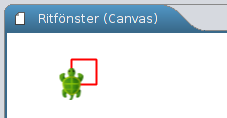
\includegraphics[width=0.47\textwidth]{../img/kojo/kvadrat}

\noindent Prova gärna olika sätt att skriva din kod \emph{utan} att resultatet ändras: skriv satser i sekvens på flera rader eller satser i sekvens på samma rad med semikolon emellan; använd blanktecken och blanka rader i koden. Hur vill du gruppera dina satser så att de är lätta för en människa att läsa?
%Prova att ändra på \emph{ordningen} mellan satserna och studera hur resultatet påverkas. Använd den \emph{gula} play-knappen  (programspårning) för att studera exekveringen i detalj. Vad händer du klickar på satser i ditt program och på rutor i programspårningen?


\Subtask Rita en trappa enligt bilden nedan.

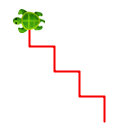
\includegraphics[width=0.3\textwidth]{../img/kojo/stairs}

\Subtask Rita valfri bild på valfri bakgrund med hjälp av några av procedurerna i tabellen nedan. Du kan till exempel rita en rosa triangel med lila konturer mot svart bakgrund. % \ref{lab:kojo:kojo-procedures}.
Försök att underlätta läsbarheten av din kod med hjälp av lämpliga radbrytningar och gruppering av satser.


\begin{table}[H]
\begin{longtable}{l l}\small
\code|fram(100)| & Paddan går framåt 100 steg (25 om argument saknas).\\
\code|färg(rosa)| & Sätter pennans färg till rosa. \\
\code|fyll(lila)| & Sätter ifyllnadsfärgen till lila. \\
\code|fyll(genomskinlig)| & Gör så att paddan \emph{inte} fyller i något när den ritar. \\
\code|bredd(20)| & Gör så att pennan får bredden 20. \\
\code|bakgrund(svart)| & Bakgrundsfärgen blir svart. \\
\code|bakgrund2(grön,gul)| & Bakgrund med övergång från grönt till gult. \\
\code|pennaNer|  & Sätter ner paddans penna så att den ritar när den går. \\
\code|pennaUpp|  & Sänker paddans penna så att den \emph{inte} ritar när den går. \\
\code|höger(45)|   & Paddan vrider sig 45 grader åt höger. \\
\code|vänster(45)| & Paddan vrider sig 45 grader åt vänster. \\
\code|hoppa|       & Paddan hoppar 25 steg utan att rita. \\
\code|hoppa(100)|  & Paddan hoppar 100 steg utan att rita. \\
\code|hoppaTill(100, 200)| & Paddan hoppar till läget (100, 200) utan att rita. \\
\code|gåTill(100, 200)|    & Paddan vrider sig och går till läget (100, 200). \\
\code|öster|   & Paddan vrider sig så att nosen pekar åt höger. \\
\code|väster|  & Paddan vrider sig så att nosen pekar åt vänster. \\
\code|norr|    & Paddan vrider sig så att nosen pekar uppåt. \\
\code|söder|   & Paddan vrider sig så att nosen pekar neråt. \\
\code|mot(100,200)|   & Paddan vrider sig så att nosen pekar mot läget (100, 200) \\
\code|sättVinkel(90)| & Paddan vrider nosen till vinkeln 90 grader. \\
\end{longtable}
%\label{lab:kojo:kojo-procedures}
%\caption{Några användbara procedurer i Kojo.}
\end{table}

\begin{framed}
\noindent\emph{Tips inför fortsättningen:} Ha gärna både REPL och Kojo igång samtidigt. Då kan du undersöka hur olika kodkonstruktioner fungerar i REPL, medan du stegvis skapar allt större program i editorn i Kojo. Detta sätt att jobba har du nytta av under resten av kursen, både om du använder en texteditor och kompilerar i terminalen, och om du använder en professionell integrerad utvecklingsmiljö. Oavsett vilka andra verktyg du kör är det användbart att ha REPL igång i ett eget fönster som hjälp i den kreativa processen, medan du jagar buggar och medan du lär dig nya koncept. Så fort du undrar hur något fungerar i Scala: fram med REPL och testa!
\end{framed}


\SOLUTION

\TaskSolved \what

\SubtaskSolved Genom att börja din Kojo-program med \code{sudda} så startar du exekveringen i samma utgångsläge: en tom rityta \Eng{canvas} där paddan pekar uppåt, pennan är nere och pennans färg är röd.  Då blir det lättare att resonera om vad programmet gör från början till slut, jämfört med om exekveringen beror på resultatet av tidigare exekveringar.


\SubtaskSolved
\begin{Code}
sudda

fram; vänster
fram; vänster
fram; vänster
fram; vänster
\end{Code}


\SubtaskSolved
\begin{Code}
sudda

fram; vänster
fram; höger

fram; vänster
fram; höger

fram; vänster
fram; höger

fram; vänster
\end{Code}


\QUESTEND









\clearpage

\ExtraTasks %%%%%%%%%%%%%%%%%% EXTRAUPPGIFTER



\WHAT{Typ och värde.}

\QUESTBEGIN

\Task \what~Vilket värde och vilken typ hör till vilket uttryck?  Är du osäker på svaret, testa i REPL.

\begin{ConceptConnections}[0.3\textwidth]
  \code|1.0 + 18          | & 1 & & A & \code|42.0: Double    | \\ 
  \code|(41 + 1).toDouble | & 2 & & B & \code|65: Int         | \\ 
  \code|1.042e42 + 1      | & 3 & & C & \code|19.0: Double    | \\ 
  \code|12E6.toLong       | & 4 & & D & \code|12000000: Long  | \\ 
  \code|32.toChar.toString| & 5 & & E & \code|'*': Char       | \\ 
  \code|'A'.toInt         | & 6 & & F & \code|48: Int         | \\ 
  \code|0.toInt           | & 7 & & G & \code|" ": String   | \\ 
  \code|'0'.toInt         | & 8 & & H & \code|1.042E42: Double| \\ 
  \code|'9'.toInt         | & 9 & & I & \code|'q': Char       | \\ 
  \code|'A' + '0'         | & 10 & & J & \code|113: Int        | \\ 
  \code|('A' + '0').toChar| & 11 & & K & \code|0: Int          | \\ 
  \code|"*!%#".charAt(0)| & 12 & & L & \code|57: Int         | \\ 
\end{ConceptConnections}

\SOLUTION

\TaskSolved \what

\begin{ConceptConnections}
  \code|1.0 + 18          | & 1 & ~~\Large$\leadsto$~~ &  E & \code|19.0: Double    | \\ 
  \code|(41 + 1).toDouble | & 2 & ~~\Large$\leadsto$~~ &  L & \code|42.0: Double    | \\ 
  \code|1.042e42 + 1      | & 3 & ~~\Large$\leadsto$~~ &  A & \code|1.042E42: Double| \\ 
  \code|12E6.toLong       | & 4 & ~~\Large$\leadsto$~~ &  K & \code|12000000: Long  | \\ 
  \code|32.toChar.toString| & 5 & ~~\Large$\leadsto$~~ &  G & \code|" ": String   | \\ 
  \code|'A'.toInt         | & 6 & ~~\Large$\leadsto$~~ &  H & \code|65: Int         | \\ 
  \code|0.toInt           | & 7 & ~~\Large$\leadsto$~~ &  I & \code|0: Int          | \\ 
  \code|'0'.toInt         | & 8 & ~~\Large$\leadsto$~~ &  F & \code|48: Int         | \\ 
  \code|'9'.toInt         | & 9 & ~~\Large$\leadsto$~~ &  D & \code|57: Int         | \\ 
  \code|'A' + '0'         | & 10 & ~~\Large$\leadsto$~~ &  B & \code|113: Int        | \\ 
  \code|('A' + '0').toChar| & 11 & ~~\Large$\leadsto$~~ &  J & \code|'q': Char       | \\ 
  \code|"*!%#".charAt(0)| & 12 & ~~\Large$\leadsto$~~ &  C & \code|'*': Char       | \\ 
\end{ConceptConnections}

%\Subtask \code{1.0 + 18}
%
%\Subtask \code{(41 + 1).toDouble}
%
%\Subtask \code{1.042e42 + 1}
%
%\Subtask \code{12E6.toLong}
%
%\Subtask \code{"gurk" + 'a'}
%
%\Subtask \code{32.toChar.toString}
%
%\Subtask \code{'A'.toInt}
%
%\Subtask \linebreak[0] \code{'0'.toInt}
%
%\Subtask \code{'0'.toInt}
%
%\Subtask \code{'9'.toInt}
%
%\Subtask \code{'A' + '0'}
%
%\Subtask \code{('A' + '0').toChar}
%
%\Subtask \code{"*!%#".charAt(0)}
%%%%%%%%%%%%%%%%%%%%%%%%%%%%%%%%%%%%%%%%%%%%%%%%
%\SubtaskSolved \code{Double, 19}
%
%\SubtaskSolved \code{Double, 42}
%
%\SubtaskSolved \code{Double, 1.042E42}
%
%\SubtaskSolved \code{Long, 12000000}
%
%\SubtaskSolved \code{String, gurka}
%
%\SubtaskSolved \code{String, " "}
%
%\SubtaskSolved \code{Int, 65}
%
%\SubtaskSolved \code{Int, 48}
%
%\SubtaskSolved \code{Int,49}
%
%\SubtaskSolved \code{Int,57}
%
%\SubtaskSolved \code{Int, 113}
%
%\SubtaskSolved \code{Char, 'q'}
%
%\SubtaskSolved \code{Char, '*'}


\QUESTEND




\WHAT{Satser och uttryck.}

\QUESTBEGIN

\Task \what

\Subtask Vad är det för skillnad på en sats och ett uttryck?

\Subtask Ge exempel på satser som inte är uttryck?

\Subtask Förklara vad som händer för varje evaluerad rad:
\begin{REPL}
scala> def värdeSaknas = ()
scala> värdeSaknas
scala> värdeSaknas.toString
scala> println(värdeSaknas)
scala> println(println("hej"))
\end{REPL}

\Subtask Vilken typ har literalen \code{()}?

\Subtask Vilken returtyp har \code{println}?

\SOLUTION

\TaskSolved \what

\SubtaskSolved  Ett utryck kan evalueras och resulterar då i ett användbart värde. En sats \emph{gör} något (t.ex. skriver ut något), men resulterat inte i något användbart värde.

\SubtaskSolved \code{println()}

\SubtaskSolved

 \code{värdeSaknas} innehåller Unit

 Skriver ut \code{Unit}

 Skriver ut \code{"()"}

 Skriver ut \code{"()"}

 Skriver först ut hej med det innersta anropet och sen \code{()} med det yttre anropet

\SubtaskSolved  \code{Unit}

\SubtaskSolved  \code{Unit}

\QUESTEND



\WHAT{Procedur med parameter.}

\QUESTBEGIN

\Task \what~En procedur är en funktion som orsakar en effekt, till exempel en utskrift eller en variabeltilldelning, men som inte returnerar något intressant resultatvärde.%
\footnote{I Scala är procedurer funktioner som returnerar det \emph{tomma värdet}, vilket skrivs \code{()} och är av typen \code{Unit}. I Java och flera andra språk finns inget tomt värde och man har en specialsyntax för procedurer som använder nyckelordet \code{void}. }

\Subtask Deklarera en förändringsbar variabel \code{highscore} som initieras till 0.

\Subtask Deklarera en procedur \code{updateHighscore} som tar en parameter \code{points} och tilldelar \code{highscore} ett nytt värde om \code{points} är större än \code{highscore} och skriver ut strängen \code{"REKORD!"}. Om inte \code{points} är större än \code{highscore} ska strängen \code{"GE INTE UPP!"} skrivas ut. Testa proceduren i REPL.

\Subtask Gör en ny variant av \code{updateHighscore}, som \emph{inte} är en procedur utan i stället är en funktion som ger en sträng för senare utskrift. Testa funktionen i REPL.

\SOLUTION

\TaskSolved \what

\SubtaskSolved
\begin{Code}
var highscore = 0
\end{Code}

\SubtaskSolved
\begin{Code}
def updateHighscore(points: Int): Unit =
  if points > highscore then
    highscore = points
    println("REKORD!")
  else println("GE INTE UPP!")
\end{Code}

\SubtaskSolved
\begin{Code}
def updateHighscore(points: Int): String =
  if points > highscore then
    highscore = points
    "REKORD!"
  else "GE INTE UPP!"
\end{Code}



\QUESTEND


\WHAT{Flyttalsaritmetik.}

\QUESTBEGIN

\Task \what

\Subtask Vilket är det minsta positiva värdet av typen \code{Double}?

\Subtask Vad är värdet av detta uttryck? Varför blir det så?
\begin{REPL}
scala> Double.MaxValue + Double.MinPositiveValue == Double.MaxValue
\end{REPL}

\SOLUTION

\TaskSolved \what

\SubtaskSolved

\begin{REPL}
scala> Double.MinPositiveValue
res0: Double = 4.9E-324
\end{REPL}

\SubtaskSolved

\begin{REPL}
scala> Double.MaxValue + Double.MinPositiveValue == Double.MaxValue
res2: Boolean = true
\end{REPL}

\QUESTEND



\WHAT{\code{if}\textit{-sats}.}

\QUESTBEGIN

\Task \what~För varje rad nedan, beskriv vad som skrivs ut.  % Uppgift 18
\begin{REPL}
scala> if !true then println("sant") else println("falskt")
scala> if !false then println("sant") else println("falskt")
scala> def singlaSlant = if math.random() < 0.5 then "krona" else "klave"
scala> for i <- 1 to 5 do print(s"$i:$singlaSlant ")
\end{REPL}

\SOLUTION

\TaskSolved \what

\begin{enumerate}
\item Utskrift: \code{falskt}
\item Utskrift: \code{sant}
\item Inget skrivs ut, funktionen deklareras men körs ej.
\item Utskrift: \code{1:krona 2:klave 3:krona 4:krona 5:klave } eller liknande beroende på vilka slumptal \code{math.random()} ger.
\end{enumerate}

\QUESTEND




\WHAT{\code{if}\textit{-uttryck}.}

\QUESTBEGIN

\Task  Deklarera följande variabler med nedan initialvärden:

\begin{REPLnonum}
scala> var grönsak = "gurka"
scala> var frukt = "banan"
\end{REPLnonum}

Ange för varje rad nedan vad uttrycket har för värde och typ:
\begin{REPLnonum}
scala> if grönsak == "tomat" then "gott" else "inte gott"
scala> if frukt == "banan" then "gott" else "inte gott"
scala> if true then grönsak else 42
scala> if false then grönsak else 42
\end{REPLnonum}

\SOLUTION


\TaskSolved \what~Notera typen \code{Any} på de sista två uttrycken.

\begin{REPLnonum}
scala> if grönsak == "tomat" then "gott" else "inte gott"
res0: String = inte gott

scala> if frukt == "banan" then "gott" else "inte gott"
res1: String = gott

scala> if true then grönsak else 42
res2: Any = gurka

scala> if false then grönsak else 42
res3: Any = 42
\end{REPLnonum}


\QUESTEND





\WHAT{Modulo-operatorn {\tt \%} och Booleska värden.}

\QUESTBEGIN

\Task \what

\Subtask Deklarera en funktion \code{def isEven(n: Int): Boolean = ???} som ger \code{true} om talet \code{n} är jämnt, annars \code{false}.

\Subtask Deklarera en funktion \code{def isOdd(n: Int): Boolean = ???} som ger \code{false} om talet \code{n} är jämnt, annars \code{true}.

\SOLUTION


\TaskSolved \what

\SubtaskSolved
\begin{REPL}
scala> def isEven(n: Int): Boolean = n % 2 == 0

scala> isEven(42)
res0: Boolean = true

scala> isEven(43)
res1: Boolean = false

\end{REPL}


\SubtaskSolved
\begin{REPL}
scala> def isOdd(n: Int): Boolean = !isEven(n)

scala> isOdd(42)
res2: Boolean = false

scala> isOdd(43)
res3: Boolean = true
\end{REPL}


\QUESTEND





\WHAT{Skillnader mellan \code{var}, \code{val}, \code{def}.}

\QUESTBEGIN

\Task \what~

\Subtask
 Evaluera varje rad en i taget i tur och ordning i Scala REPL. För varje rad nedan: förklara för vad som händer och notera värde och ev fel. % Uppgift 15
\begin{REPL}
scala> var x = 30
scala> x + 1
scala> x = x + 1
scala> x == x + 1
scala> val y = 20
scala> y = y + 1
scala> var z = { println("hej z!"); math.random() }
scala> def w = { println("hej w!"); math.random() }
scala> z
scala> z
scala> z = z + 1
scala> w
scala> w
scala> w = w + 1
\end{REPL}


\Subtask Vad är det för skillnad på \code{var}, \code{val} och \code{def}?



\SOLUTION

\TaskSolved \what

\SubtaskSolved
\begin{REPL}
  scala> var x = 30
  x: Int = 30

  scala> x + 1
  res6: Int = 31

  scala> x = x + 1
  x: Int = 31

  scala> x == x + 1
  res7: Boolean = false

  scala> val y = 20
  y: Int = 20

  scala> y = y + 1
  <console>:12: error: reassignment to val
         y = y + 1
           ^

  scala> var z = { println("hej z!"); math.random() }
  hej z!
  z: Double = 0.3381365875903367

  scala> def w = { println("hej w!"); math.random() }
  w: Double

  scala> z
  res8: Double = 0.3381365875903367

  scala> z
  res9: Double = 0.3381365875903367

  scala> z = z + 1
  z: Double = 1.3381365875903368

  scala> w
  hej w!
  res10: Double = 0.06420209879434557

  scala> w
  hej w!
  res11: Double = 0.5777951341051852

  scala> w = w + 1
  <console>:12: error: value w_= is not a member of object
         w = w + 1
\end{REPL}


\SubtaskSolved
\begin{itemize}
\item \code{var namn = uttryck} används för att deklarera en förändringsbar variabel. Namnet kan med hjälp av en tilldelningssats referera till nya värden.

\item \code{val namn = uttryck} används för att deklarera en oföränderlig variabel som efter initialisering inte kan förändras med tilldelningssatser. Vid försök ges kompileringsfel.
\item \code{def namn = uttryck} används för att deklarera en funktion vars uttryck evalueras varje gång den anropas.
\end{itemize}

\QUESTEND




\WHAT{Skillnaden mellan \code{if} och \code{while}.}

\QUESTBEGIN

\Task \what~Vad blir resultatet av rad 3 och 4?

\begin{REPL}
scala> def lotto1 = if math.random() > 0.5 then print("vinst :) ")
scala> def lotto2 = while math.random() > 0.5 do print("vinst :) ")
scala> lotto1
scala> lotto2
\end{REPL}

\SOLUTION

\TaskSolved \what

\begin{itemize}
\item Rad 3: Har du tur (50\% chans) får du vinst en gång.

\item Rad 4: Har du tur får du många vinster i rad. Sannolikheten för $n$ vinster i rad är $(\frac{1}{2})^n$.
\end{itemize}
\QUESTEND












\clearpage

\AdvancedTasks   %%%%%%%%%%%%%%%%%%% FÖRDJUPNINGSUPPGIFTER





\WHAT{Logik och De Morgans Lagar.}

\QUESTBEGIN

\Task \what~Förenkla följande uttryck. Antag att \code{poäng} och \code{highscore} är heltalsvariabler medan \code{klar} är av typen \code{Boolean}.
  % Uppgift 24

\Subtask \code{poäng > 100 && poäng > 1000}

\Subtask \code{poäng > 100 || poäng > 1000}

\Subtask \code{!(poäng > highscore)}

\Subtask \code{!(poäng > 0 && poäng < highscore) }

\Subtask \code{!(poäng < 0 || poäng > highscore) }

\Subtask \code{klar == true}

\Subtask \code{klar == false}

\SOLUTION

\TaskSolved \what


\SubtaskSolved \code{poäng > 1000}

\SubtaskSolved \code{poäng > 100}

\SubtaskSolved \code{poäng <= highscore}

\SubtaskSolved \code{poäng <= 0 || poäng >= highscore }

\SubtaskSolved \code{poäng >= 0 && poäng <= highscore}

\SubtaskSolved \code{klar}

\SubtaskSolved \code{!klar}


\QUESTEND






\WHAT{Stränginterpolatorn \code{s}.}

\QUESTBEGIN

\Task \what~Med ett \code{s} framför en strängliteral får man hjälp av kompilatorn att, på ett typsäkert sätt, infoga variabelvärden i en sträng.
Variablernas namn ska föregås med ett dollartecken , t.ex. \code{s"Hej $namn"}.
Om man vill evaluera ett uttryck placeras detta inom klammer direkt efter dollartecknet, t.ex.
\code/s"Dubbla längden: ${namn.size * 2}"/

\Subtask Vad skrivs ut nedan?
\begin{REPL}
scala> val f = "Kim"
scala> val e = "Finkodare"
scala> println(s"Namnet '$f $e' har ${f.size + e.size} bokstäver.")
\end{REPL}

\Subtask Skapa följande utskrifter med hjälp av stränginterpolatorn \code{s} och variablerna \code{f} och \code{e} i föregående deluppgift.
\begin{REPL}
Kim har 3 bokstäver.
Finkodare har 9 bokstäver.
\end{REPL}

\SOLUTION

\TaskSolved \what

\SubtaskSolved
\begin{REPLnonum}
Namnet 'Kim Finkodare' har 12 bokstäver.
\end{REPLnonum}

\SubtaskSolved
\begin{REPLnonum}
println(s"$f har  ${f.size} bokstäver.")
println(s"$e har  ${e.size} bokstäver.")
\end{REPLnonum}

\QUESTEND



\WHAT{Tilldelningsoperatorer.}

\QUESTBEGIN

\Task \what~Man kan förkorta en tilldelningssats som förändrar en variabel, t.ex. \code{x = x + 1}, genom att använda så kallade tilldelningsoperatorer och skriva \code{x += 1} som betyder samma sak. Rita en ny bild av datorns minne efter varje rad nedan. Bilderna ska visa variablers namn, typ och värde.

\begin{REPL}
scala> var a = 40
scala> var b = a + 40
scala> a += 10
scala> b -= 10
scala> a *= 2
scala> b /= 2
\end{REPL}

\SOLUTION

\TaskSolved \what

\begin{tabular}{l l}
\MEM{{\it Efter rad1:~~~~} a}{Int}{40}\\
\MEM{{\it Efter rad2:~~~~} a}{Int}{40} & \MEM{b}{Int}{80}\\
\MEM{{\it Efter rad3:~~~~} a}{Int}{50} & \MEM{b}{Int}{80}\\
\MEM{{\it Efter rad4:~~~~} a}{Int}{50} & \MEM{b}{Int}{70} \\
\MEM{{\it Efter rad5:~~~~} a}{Int}{100} & \MEM{b}{Int}{70} \\
\MEM{{\it Efter rad6:~~~~} a}{Int}{100} & \MEM{b}{Int}{35} \\
\end{tabular}

\QUESTEND






\WHAT{Stora tal.}

\QUESTBEGIN

\Task \what~Om vi vill beräkna $2^{64} -1$ som ett exakt heltal\footnote{\url{https://en.wikipedia.org/wiki/Wheat_and_chessboard_problem}} blir det större än \code{Int.MaxValue}, så vi kan tyvärr inte använda snabba \code{Int}. Till vår räddning: \code{BigInt}

\Subtask Läs om \code{BigInt} och \code{BigDecimal} på \Scaladoc \\ Notera vad de kan användas till.

\Subtask Du skapar ett \code{BigInt}-heltal med \code{BigInt(2)} och kan anropa funktionen \code{pow} på en \code{BigInt} med punktnotation. Beräkna $2^{64} -1$ som ett exakt heltal.

\Subtask Vilka nackdelar finns med \code{BigInt} och \code{BigDecimal}?

\SOLUTION

\TaskSolved \what

\SubtaskSolved \code{BigInt} kan användas i stället för \code{Int} vid mycket stora heltal. Det finns förståss även \code{Long} som har dubbelt omfång jämfört med \code{Int}, medan \code{BigInt} kan ha godtyckligt många siffror (ända tills minnet tar slut) och kan därmed representera ofantligt stora tal. \code{BigDecimal} kan användas i stället för \code{Double} vid mycket stora decimaltal.

\SubtaskSolved
\begin{REPL}
scala> BigInt(2).pow(64)
res0: scala.math.BigInt = 18446744073709551616
\end{REPL}

\SubtaskSolved Beräkningar går mycket långsammare och de är lite krångligare att använda.

\QUESTEND





\WHAT{Precedensregler}

\QUESTBEGIN

\Task \what~Evalueringsordningen kan styras med parenteser. Vilket värde och vilken typ har följande uttryck?

\Subtask \code{23 + 2 * 2 + (23 + 2) * 2}

\Subtask \code{(-(2 - 42)) / (1 + 1 + 1)}

\Subtask \code{(-(2 - 42)) / (-1)/(1 + 1 + 1)}

\SOLUTION

\TaskSolved \what

\SubtaskSolved \code{77:  Int}

\SubtaskSolved \code{13: Int}

\SubtaskSolved \code{-13: Int}

\QUESTEND



\WHAT{Dokumentation av paket i Java och Scala.}

\QUESTBEGIN

\Task \what


\Subtask Genom att trycka på tab tangenten kan man se vad som finns i olika paket. Vad heter konstanten $\pi$  i \code{java.lang.Math} (notera stort M) respektive \code{scala.math.}?

\begin{REPL}
scala> java.lang.Math.    //tryck TAB efter punkten
scala> scala.math.        //tryck TAB efter punkten
\end{REPL}

\Subtask Jämför dokumentationen för klassen \code{java.lang.Math} här: \\ \url{https://docs.oracle.com/javase/8/docs/api/} \\
med dokumentationen för paketet \code{scala.math} här: \\
\url{http://www.scala-lang.org/api} \\
Ge exempel på vad man kan göra på webbsidan med Scala-dokumentationen som man \emph{inte} kan göra i motsvarande webbsida Java-dokumentation.

\Subtask Vad gör metoden \code{hypot}? Vad är det som är bra med att använda \code{hypot} i stället för att själv implementera beräkningen med hjälp av kvadratrot, multiplikation och addition?

\SOLUTION

\TaskSolved \what

\SubtaskSolved Scala: \code{Pi}, Java: \code{PI}

\SubtaskSolved Man kan söka och filtrera fram alla förekomster av en viss teckenkombination.

\SubtaskSolved Räknar ut hypotenusan (Pythagoras sats) utan risk för avrundningsproblem i mellanberäkningar.


\QUESTEND





\WHAT{Noggrannhet och undantag i aritmetiska uttryck.}

\QUESTBEGIN

\Task \what~Vad blir resultatet av uttrycken nedan? Notera undantag \Eng{exceptions} och noggrannhetsproblem.

\Subtask \code{Int.MaxValue + 1}

\Subtask \code{1 / 0}

\Subtask \code{1E8 + 1E-8}

\Subtask \code{1E9 + 1E-9}

\Subtask \code{math.pow(math.hypot(3,6), 2)}

\Subtask\Uberkurs \code{1.0 / 0}

\Subtask\Uberkurs \code{(1.0 / 0).toInt}

\Subtask\Uberkurs \code{math.sqrt(-1)}

\Subtask\Uberkurs \code{math.sqrt(Double.NaN)}

\Subtask \code{throw new Exception("PANG!!!")}

\SOLUTION

\TaskSolved \what

\SubtaskSolved \code{-2147483648} vilket motsvarar \code{Int.MinValue}.

\SubtaskSolved Ett undantag kastas: \code{java.lang.ArithmeticException: / by zero}

\SubtaskSolved \code{1.0000000000000001E8} (som förväntat)

\SubtaskSolved Avrundas till \code{1E9} (flyttalsaritmetik med noggrannhetsproblem: ett stort flyttal plus ett (alltför) litet flyttal kan ge samma tal. Det lilla talet ''försvinner'').


\SubtaskSolved \code{45.00000000000001} (flyttalsaritmetik med noggrannhetsproblem: enligt ''normal'' aritmetik ska det bli exakt 45.)

\SubtaskSolved \code{Infinity} (som även ges av \code{Double.PositiveInfinity} och som representerar den positiva oändligheten).

\SubtaskSolved \code{2147483647} vilket motsvarar \code{Int.MaxValue}.

\SubtaskSolved \code{NaN} vilket betyder ''Not a Number''.

\SubtaskSolved \code{NaN} vilket betyder ''Not a Number''.

\SubtaskSolved Ett undantag kastas: \code{java.lang.Exception: PANG!!!}

\QUESTEND



\WHAT{Modulo-räkning med negativa tal.}

\QUESTBEGIN

\Task\Uberkurs \what~Läs om moduloräkning här: \\
 \href{https://en.wikipedia.org/wiki/Modulo\_operation}{en.wikipedia.org/wiki/Modulo\_operation} \\
 och undersök hur det blir med olika tecken (positivt resp. negativt) på moduloräkning med $dividend \% divisor$ i Scala.


\SOLUTION

\TaskSolved \what~I Scala har resultatet samma tecken som dividenden.
\begin{REPL}
scala> 1 % 2
res0: Int = 1

scala> -1 % 2
res1: Int = -1

scala> -1 % -2
res2: Int = -1

scala> 1 % -2
res3: Int = 1

\end{REPL}

\QUESTEND




\WHAT{Bokstavliga identifierare.}

\QUESTBEGIN

\Task\Uberkurs \what~Läs om identifierare i Scala och speciellt \emph{literal identifiers} här: \url{http://www.artima.com/pins1ed/functional-objects.html#6.10}.

\Subtask Förklara vad som händer nedan:
\begin{REPLnonum}
scala> val `bokstavlig val` = 42
scala> println(`bokstavlig val`)
\end{REPLnonum}

\Subtask Scala och Java har olika uppsättningar med reserverade ord. På vilket sätt kan ''backticks'' vara använbart med anledning av detta?

\SOLUTION

\TaskSolved \what

\SubtaskSolved Variabeln får namnet 'bokstavlig val', bakåt-apostrofer \Eng{backticks} gör att man kan namnge variabler till annars otillåtna namn, t.ex. med mellanrum eller nyckelord i sig.

\SubtaskSolved Backticks i Scala möjliggör alla möjliga tecken i namn. Exempel på användning: I java finns en metod som heter \jcode{java.lang.Thread.yield} men i Scala är yield ett nyckelord; för att komma runt det går det att i Scala skriva \jcode{java.lang.Thread.`yield`}

\QUESTEND












\WHAT{\code{java.lang.Integer}, hexadecimala litteraler, BigDecimal.}

\QUESTBEGIN

\Task\Uberkurs \what~

\Subtask Sök upp dokumentationen för \code{java.lang.Integer}.\\Använd metoderna \code{toBinaryString} och \code{toHexString} för att fylla i tabellen nedan.

\begin{table}[H]
\begin{tabular}{l | l | l}
decimalt heltal & binärt värde & hexadecimalt värde \\
\hline
$33$ &   &  \\
$42$ &   &  \\
$64$ &   &  \\
\end{tabular}
\end{table}

\Subtask Hur anger man det hexadecimala heltalsvärdet 10c (motsvarar 268 decimalt) som en litteral i Scala?

\Subtask Vad blir \code{0x10} upphöjt till $c =$ ljusets hastighet i $m/s$? \emph{Tips:} Använd \code{BigDecimal}.

\SOLUTION

\TaskSolved \what

\SubtaskSolved

\begin{REPL}
scala> import Integer.{toBinaryString => toBin, toHexString => toHex}

scala> for i <- Seq(33, 42, 64) do println(s"$i \t ${toBin(i)} \t ${toHex(i)}")
33 	 100001 	 21
42 	 101010 	 2a
64 	 1000000 	 40
\end{REPL}


\SubtaskSolved Det hexadecimala heltalet $10c$ kan anges med litteralen \code{0x10c} i Scala, Java och många andra språk: \footnote{\url{https://en.wikipedia.org/wiki/0x10c}}
\begin{REPL}
scala> 0x10c
res0: Int = 268
\end{REPL}

\SubtaskSolved \footnote{\url{https://c418.bandcamp.com/album/0x10c}}
\begin{REPL}
scala> val c = 299792458
c: Int = 299792458

scala> BigDecimal(0x10).pow(c)
res68: scala.math.BigDecimal = 2.124892963227906613060986110887672E+360986089
\end{REPL}


\QUESTEND









\WHAT{Strängformatering.}

\QUESTBEGIN

\Task\Uberkurs \what~Läs om \code{f}-interpolatorn här:\\
\url{http://docs.scala-lang.org/overviews/core/string-interpolation.html} \\
Hur kan du använda \code{f}-interpolatorn för att göra följande utskrift i REPL? Ändra rad 3 vid \code{???} så att flyttalet \code{g} avrundas till tre decimaler innan utskrift sker.
\begin{REPL}
scala> val g = 2 / 3.0
scala> val str = f"Jättegurkan är $g??? meter lång"
scala> println(str)
Jättegurkan är 0.667 meter lång
\end{REPL}

\SOLUTION

\TaskSolved \what

\begin{Code}
val str = f"Jättegurkan är $g%1.3f meter lång"
\end{Code}
(Om du tycker att \code{$g%1.3f}
ser kryptiskt ut, så kan du trösta dig med att du nu får chansen att föra vidare ett anrikt arv från det urgamla språket C och den sägenomspunna funktionen \code{printf} till kommande generationer av invigda kodmagiker.)

\QUESTEND




\WHAT{Multiplikationsvarning.}

\QUESTBEGIN

\Task \what~Sök upp dokumentationtionen för\\\code{java.lang.Math.multiplyExact} och läs om vad den metoden gör.

\Subtask Vad händer här?

\begin{REPLnonum}
scala> Math.multiplyExact(1, 2)
scala> Int.MaxValue * 2
scala> Math.multiplyExact(Int.MaxValue, 2)
\end{REPLnonum}

\Subtask Varför kan man vilja använda \code{java.lang.Math.multiplyExact} i stället för ''vanlig'' multiplikation?

\SOLUTION

\TaskSolved \what

\SubtaskSolved Den andra multiplikationen flödar över \Eng{overflow} gränsen för största möjliga värdet av en \code{Int}. I den tredje multiplikationen kastas i stället ett undantag \code{java.lang.ArithmeticException: integer overflow}


\begin{REPLnonum}
scala> Math.multiplyExact(1, 2)
res70: Int = 2

scala> Int.MaxValue * 2
res71: Int = -2

scala> Math.multiplyExact(Int.MaxValue, 2)
java.lang.ArithmeticException: integer overflow
  at java.lang.Math.multiplyExact(Math.java:867)
  ... 42 elided
\end{REPLnonum}

\SubtaskSolved Används då man vill vara helt säker på att overflow-buggar ''smäller'' direkt i stället för att generera felaktiga resultat vars konsekvenser kanske manifesterar sig långt senare. Dock är \code{multiplyExact} aningen långsammare än vanlig multiplikation.


\QUESTEND








\WHAT{Dekorera \code{Int} med extra operatorer.}

\QUESTBEGIN

\Task\Uberkurs \what\footnote{En utmanande överkursuppgift som visar Scalas kraftfullhet. Se fördjupningslänkar i facit.}\\Kim Kodmagiker tycker att \code{Math.multiplyExact} är för krångligt att skriva och utökar därför typen \code{Int} med en extra operator:

\begin{Code}
implicit class IntDecorator(val i: Int) extends AnyVal {
  def *!(j: Int) = Math.multiplyExact(i,j)
}
\end{Code}

\Subtask Klistra in koden ovan i REPL och prova den extra operatorn.

\Subtask Hjälp Kim Kodmagiker att lägga till fler operatorer på värden av typen \code{Int}, som gör att det även går att använda \code{Math.subtractExact} och \code{Math.addExact} smidigt.

\Subtask Testa ett sammansatt uttryck som använder alla extrametoder på \code{Int}. Tycker du det blev mer lättläst eller mer kryptiskt med de nya operatorerna?

\SOLUTION

\TaskSolved \what

\SubtaskSolved

\begin{REPL}
scala> Int.MaxValue *! 1
res0: Int = 2147483647

scala> Int.MaxValue *! 2
java.lang.ArithmeticException: integer overflow
  at java.lang.Math.multiplyExact(Math.java:867)
  at IntExtra.$times$bang(<console>:16)
  ... 32 elided

\end{REPL}

Kort förklaring:
\begin{itemize}
\item \code{implicit class MinDekorator(x: Typ)} gör så att operationer i dekoratorklassen \code{MinDekorator} automatiskt görs tillgängliga på värden av typen \code{Typ}.%
\footnote{Fördjupning: \url{http://docs.scala-lang.org/overviews/core/implicit-classes.html}}

\item \code{extends AnyVal} gör så att kompilatorn försöker generera maskinkod som blir lika effektiv som vid direkt användning av det underliggande värdet.%
\footnote{Fördjupning: \url{http://docs.scala-lang.org/overviews/core/value-classes.html}}
\end{itemize}


\SubtaskSolved

\begin{Code}
implicit class IntDecorator(val i: Int) extends AnyVal{
  def *!(j: Int) = Math.multiplyExact(i,j)
  def +!(j: Int) = Math.addExact(i,j)
  def -!(j: Int) = Math.subtractExact(i,j)
}
\end{Code}


\SubtaskSolved Det blir lätt väldigt kryptiskt med namn som består av flera specialtecken. Om du \emph{verkligen} vill ha sådana operatorer är det \emph{mycket} lämpligt att också erbjuda varianter i klartext:
\begin{Code}
implicit class IntDecorator(val i: Int) extends AnyVal{
  def mulExact(j: Int) = Math.multiplyExact(i,j)
  def *!(j: Int) = i mulExact j

  def addExact(j: Int) = Math.addExact(i,j)
  def +!(j: Int) = i addExact j

  def subExact(j: Int) = Math.subtractExact(i,j)
  def -!(j: Int) = i subExact j
}

\end{Code}


\QUESTEND



%%%%%%%%%%%%%%%%%%%%%%%%%%%%%%%%%%%%%%%%%%%%%%%%
%%%%%%%%%%%%%%%%%%%%%%%%%%%%%%%%%%%%%%%%%%%%%%%%
%%%%%%%%%%%%%%%%%%%%%%%%%%%%%%%%%%%%%%%%%%%%%%%%
%%%%%%%%%%%%%%%%%%%%%%%%%%%%%%%%%%%%%%%%%%%%%%%%
%%%%%%%%%%%%%%%%%%%%%%%%%%%%%%%%%%%%%%%%%%%%%%%%
%%%%%%%%%%%%%%%%%%%%%%%%%%%%%%%%%%%%%%%%%%%%%%%%
%%%%%%%%%%%%%%%%%%%%%%%%%%%%%%%%%%%%%%%%%%%%%%%%
%%%%%%%%%%%%%%%%%%%%%%%%%%%%%%%%%%%%%%%%%%%%%%%%
%%%%%%%%%%%%%%%%%%%%%%%%%%%%%%%%%%%%%%%%%%%%%%%%


%% Saker som inte fick plats:



%\Task Läs om BigInt och BigDecimal här: \href{http://alvinalexander.com/scala/how-to-use-large-integer-decimal-numbers-in-scala-bigint-bigdecimal}{alvinalexander.com/scala/how-to-use-large-integer-decimal-numbers-in-scala-bigint-bigdecimal} och prova att skapa riktigt stora tal med hjälp av metoden \code{pow} på BigInt och tal med riktigt många decimaler med BigDecimal dess metod \code{pow}.


%
%
%\Subtask\Pen Sök med Ctrl+F i webbläsaren och efter förekomster av texten \textit{''overflow''} i javadoc för klassen \code{java.lang.Math} i JDK 8. Vad är ''overflow''? Vilka metoder finns i \code{java.lang.Math} som hjälper dig att upptäcka om det blir overflow?
%
%\Task Använda Scala REPL för att undersöka konstanterna nedan. Vilket av dessa värden är negativt? Vad kan man ha för praktisk nytta av dessa värden i ett program som gör flyttalsberäkningar?
%
%\Subtask \code{java.lang.Double.MIN_VALUE}
%
%\Subtask \code{scala.Double.MinValue}
%
%\Subtask \code{scala.Double.MinPositiveValue}
%
%\Task För typerna \code{Byte}, \code{Short}, \code{Char}, \code{Int}, \code{Long}, \code{Float}, \code{Double}: Undersök hur många bitar som behövs för att representera varje typs omfång? \\*
%\textit{Tips:} Några användbara uttryck: \\*
% \code{Integer.toBinaryString(Int.MaxValue + 1).size} \\*
% \code{Integer.toBinaryString((math.pow(2,16) - 1).toInt).size} \\*
% \code{1 + math.log(Long.MaxValue)/math.log(2)}
%Se även språkspecifikationen för Scala, kapitlet om heltalsliteraler: \\
%\url{http://www.scala-lang.org/files/archive/spec/2.11/01-lexical-syntax.html#integer-literals}
%
%\Subtask Undersök källkoden för paketobjektet \code{scala.math} här: \\
%\url{https://github.com/scala/scala/blob/v2.11.7/src/library/scala/math/package.scala} \\
%Hur många olika överlagrade varianter av funktionen \code{abs} finns det och för vilka parametertyper är den definierad?

%!TEX encoding = UTF-8 Unicode
%!TEX root = ../labs.tex

\Lab{\LabWeekONE}
%\externaldocument{compendium}
\begin{Goals}
%!TEX encoding = UTF-8 Unicode

\item Kunna kombinera principerna sekvens, alternativ, repetition, och abstraktion i skapandet av egna program om minst 20 rader kod.
\item Kunna förklara vad ett program gör i termer av sekvens, alternativ, repetition, och abstraktion.
\item Kunna tillämpa principerna sekvens, alternativ, repetition, och abstraktion i enkla algoritmer.
\item Kunna formatera egna program så att de blir lätta att läsa och förstå.
\item Kunna förklara vad en variabel är och kunna skriva deklarationer och göra tilldelningar.
\item Kunna genomföra upprepade varv i cykeln \emph{editera-exekvera-felsöka/förbättra} för att successivt bygga upp allt mer utvecklade program.

\end{Goals}

\begin{Preparations}
\item Repetera veckans föreläsningsmaterial.
\item \DoExercise{\ExeWeekONE}{01}%Gör övning {\tt \ExeWeekONE} i kapitel \ref{exe:W01}.
\item Läs om Kojo i appendix \ref{appendix:kojo}. Kojo Desktop är förinstallerat på LTH:s datorer; om du vill installera Kojo Desktop på din egen dator, följ instruktionerna i \ref{appendix:ide:kojo:install}. Du kan också köra Kojo i din webbläsare här: \url{http://kojo.lu.se/}
\item Läs igenom hela laborationen nedan. Fundera på möjliga lösningar till de uppgifter som är markerade med en penna i marginalen.
% \item Ladda hem och studera översiktligt detta dokument (25 sidor, det räcker att du bläddrar igenom dokumentet och får en uppfattning om hur Kojo kan användas): \\ ''Introduction to Kojo'' \url{http://www.kogics.net/kojo-ebooks#intro}
\end{Preparations}

\subsection{Obligatoriska uppgifter}

Om det förekommer en penna i marginalen ska du anteckna något inför redovisningen.


%%%%%%%%%%%%%%NEDAN ÄR FLYTTAT TILL ÖVNING 1 FÖR ATT GÖRA TYDLIGARE KOPPLING MELLAN LABBAR OCH ÖVN
%\Task \textit{Sekvens}.
%
%\Subtask Starta Kojo. Om du inte redan har svenska menyer: välj svenska i språkmenyn och starta om Kojo.  Skriv in nedan program och tryck på den \emph{gröna} play-knappen.
%
%\begin{Code}
%sudda
%
%fram; höger
%fram; vänster
%färg(grön)
%fram
%\end{Code}
%\noindent
%%Genom att börja din Kojo-program med \code{sudda} så startar du exekveringen i samma utgångsläge: en tom canvas där paddan pekar uppåt, pennan är nere och pennans färg är röd.
%%Då blir det lättare att resonera om vad programmet gör från början till slut, jämfört med om exekveringen beror på resultatet av tidigare exekveringar.
%
%\Subtask\Pen Vad händer om du \emph{inte} börjar programmet med \code{sudda} och kör samma program upprepade gånger? Varför är det bra att börja programmet med \code{sudda}?
%
%\Subtask Rita en kvadrat enligt bilden nedan.
%\vspace{1em}\\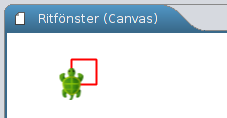
\includegraphics[width=0.45\textwidth]{../img/kojo/kvadrat}
%
%\Subtask Prova olika sätt att skriva din kod \emph{utan} att resultatet ändras: skriv satser i sekvens på flera rader eller satser i sekvens på samma rad med semikolon emellan; använd blanktecken och blanka rader i koden. Hur vill du gruppera dina satser så att de är lätta för en människa att läsa?
%
%\Subtask Prova att ändra på \emph{ordningen} mellan satserna och studera hur resultatet påverkas. Använd den \emph{gula} play-knappen  (programspårning) för att studera exekveringen i detalj. Klicka på satser i ditt program och på rutor i programspårningen och se vad som händer.
%
%
%\Subtask Rita en trappa enligt bilden nedan.
%
%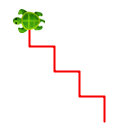
\includegraphics[width=0.2\textwidth]{../img/kojo/stairs}
%
%\Subtask Rita valfri bild på valfri bakgrund med hjälp av några av procedurerna i tabellen nedan. Du kan till exempel rita en rosa triangel med lila konturer mot svart bakgrund. % \ref{lab:kojo:kojo-procedures}.
%Försök att underlätta läsbarheten av din kod med hjälp av lämpliga radbrytningar och gruppering av satser. Undersök hur ordningen av satserna i din kod påverkar resultatet.
%
%
%
%\begin{table}[H]
%\begin{tabular}{l l}\small
%\code|fram(100)| & Paddan går framåt 100 steg (25 om argument saknas).\\
%\code|färg(rosa)| & Sätter pennans färg till rosa. \\
%\code|fyll(lila)| & Sätter ifyllnadsfärgen till lila. \\
%\code|fyll(genomskinlig)| & Gör så att paddan \emph{inte} fyller i något när den ritar. \\
%\code|bredd(20)| & Gör så att pennan får bredden 20. \\
%\code|bakgrund(svart)| & Bakgrundsfärgen blir svart. \\
%\code|bakgrund2(grön,gul)| & Bakgrund med övergång från grönt till gult. \\
%\code|pennaNer|  & Sätter ner paddans penna så att den ritar när den går. \\
%\code|pennaUpp|  & Sänker paddans penna så att den \emph{inte} ritar när den går. \\
%\code|höger(45)|   & Paddan vrider sig 45 grader åt höger. \\
%\code|vänster(45)| & Paddan vrider sig 45 grader åt vänster. \\
%\code|hoppa|       & Paddan hoppar 25 steg utan att rita. \\
%\code|hoppa(100)|  & Paddan hoppar 100 steg utan att rita. \\
%\code|hoppaTill(100, 200)| & Paddan hoppar till läget (100, 200) utan att rita. \\
%\code|gåTill(100, 200)|    & Paddan vrider sig och går till läget (100, 200). \\
%\code|öster|   & Paddan vrider sig så att nosen pekar åt höger. \\
%\code|väster|  & Paddan vrider sig så att nosen pekar åt vänster. \\
%\code|norr|    & Paddan vrider sig så att nosen pekar uppåt. \\
%\code|söder|   & Paddan vrider sig så att nosen pekar neråt. \\
%\code|mot(100,200)|   & Paddan vrider sig så att nosen pekar mot läget (100, 200) \\
%\code|sättVinkel(90)| & Paddan vrider nosen till vinkeln 90 grader. \\
%\end{tabular}
%%\label{lab:kojo:kojo-procedures}
%%\caption{Några användbara procedurer i Kojo.}
%\end{table}


%%% NEDAN ÄR BORTTAGEN FÖR ATT MINSKA MÄNGDEN ARBETE

%\Subtask \emph{Rita och mät}.
%\begin{itemize}[noitemsep]
%\item Börja ditt program med dessa satser:\\ \code{sudda; axesOn; gridOn; sakta(0); osynlig}
%\item Rita sedan en kvadrat som har 444 längdenheter i omkrets.
%\item Ta fram linjalen med höger-klick i ritfönstret och mät så exakt du kan hur lång diagonalen i kvadraten är. Skriv ner resultatet. \\ \emph{Tips:} Du kan zooma med mushjulet om du håller nere Ctrl-knappen. Du kan flytta linjalen om du klick-drar på linjalens skalstreck. Du kan vrida linjalen om du klickar på skalstrecken och håller nere Shift-tangenten.
%\item Kontrollera med hjälp av \code{math.hypot} och \code{println} vad det exakta svaret är. Skriv ner svaret med 3 decimalers noggrannhet. Du kan t.e.x. använda REPL i ett terminalfönster bredvid, eller öppna ett nytt extra Kojo-fönster i Arkiv-menyn, eller lägga in utskrifterna sist i ditt befintliga program. Utskrifter med \code{println} i Kojo sker i utdatafönstret.
%\end{itemize}
%
%\Subtask Rita en liksidig triangel med sidan 300 längdenheter genom att ge lämpliga argument till \code{fram} och \code{höger}. Vinklar anges i grader.
%
%\Subtask\Checkpoint Visa dina resultat för en handledare och diskutera hur uppgifterna ovan illustrerar principen om sekvens.

\vspace{1em}

% \Task Läs om hur du gör grafikprogram med Kojo i Appendix \ref{appendix:kojo} och övning {\tt \ExeWeekONE} i kapitel \ref{exe:W01}.


\Task \textit{Sekvens och repetition}. Rita en kvadrat med hjälp av \code+upprepa(n){ ??? }+ där du ersätter \code{n} med antalet repetitioner och \code{???} med de satser som ska repeteras.

%\Subtask Om du kör Kojo Desktop: Prova att köra ditt program med den \emph{gula} play-knappen för programspårning. Studera exekveringssekvensen. Klicka på anropen i programspårningsfönstret och studera markeringarna i ritfönstret.





\Task \textit{Variabel och repetition}.

\Subtask Funktionen \code{System.currentTimeMillis} ingår i Javas standardbibliotek och ger ett heltal av typen \code{Long} med det nuvarande antalet millisekunder sedan midnatt den första januari 1970.  Med Kojo-proceduren \code{sakta(0)} blir det ingen fördröjning när paddan ritar och utritningen sker så snabbt som möjligt. Prova nedan program och förklara vad som händer.
\begin{Code}
sakta(0)
val n = 800 * 4
val t1 = System.currentTimeMillis
upprepa(n){ upprepa(4){ fram; höger } }
val t2 = System.currentTimeMillis
println(s"$n kvadratvarv tog ${t2 - t1} millisekunder")
\end{Code}
\noindent Om du kör Kojo Desktop är det bra att börjar programmet med \code{sudda}. (Varför?)

\Subtask\Pen Anteckna ungefär hur många kvadratvarv per sekund som paddan kan rita när den är som snabbast. Kör flera gånger eftersom den virtuella maskinen behöver ''värmas upp'' för att maskinkoden ska optimeras. Vissa körningar kan gå långsammare om skräpsamlaren behöver lägga tid på att frigöra minne.

\Subtask\Pen Vad har variablerna i koden ovan för namn? Vad har variablerna för värden?

\Subtask Rita en kvadrat igen, men nu med hjälp av en \code{while}-sats och en loopvariabel. %Studera exekveringen med programspårning (den gula play-knappen).

\begin{Code}
sakta(100)
var i = 0
while (???) { fram; höger; i = ??? }
\end{Code}

\Subtask\Pen Vad är det för skillnad på variabler som deklareras med \code{val} respektive \code{var}?

\Subtask Rita en kvadrat igen, men nu med hjälp av en \code{for}-sats. Skriv ut värdet på den lokala variabeln \code{i} i varje loop-runda.

\begin{Code}
for (i <- 1 to ???) { ??? }
\end{Code}

\Subtask\Pen Går det att tilldela variabeln \code{i} ett nytt värde i loopen?

\Subtask\Pen Går det att referera till namnet \code{i} utanför loopen?


\Subtask Rita en kvadrat igen, men nu med hjälp av \code{foreach}. Skriv ut loopvariabelns värde i varje runda.

\begin{Code}
(1 to ???).foreach{ i => ??? }
\end{Code}

%\Subtask\Pen För var och en av de fyra repetitionskonstruktionerna du sett ovan, \code{upprepa}, \code{while}, \code{for} och \code{foreach}: skriv kod med penna på papper som skriver ut de första 100 jämna heltalen med blanktecken emellan: \code{2 4 6 8 10 12 ...} etc.\\ Vilken typ av loop tycker du är enklast att använda i detta fall?


\Task \textit{Abstraktion}.

\Subtask Använd en repetition för att abstrahera nedan sekvens, så att programmet blir kortare:
\begin{Code}
fram; höger; hoppa; fram; vänster; hoppa; fram; höger;
hoppa; fram; vänster; hoppa; fram; höger; hoppa; fram;
vänster; hoppa; fram; höger; hoppa; fram; vänster; hoppa;
fram; höger; hoppa; fram; vänster; hoppa
\end{Code}

%\Subtask\Pen Sök på nätet efter ''DRY principle programming'' och beskriv med egna ord vad DRY betyder och varför det är en viktig princip.

\Subtask Definiera en egen procedur som heter \code{kvadrat} med hjälp av nyckelordet \code{def} som vid anrop ritar en kvadrat med hjälp av en \code{for}-loop.

\begin{Code}
def kvadrat = for (???) {???}
\end{Code}


\Subtask Anropa din abstraktion efter att den deklarerats och efter att du exekverat:\\\code{sakta(100)}


\Subtask Anropa din abstraktion inuti en \code{for}-loop så att paddan ritar en stapel som är 10 kvadrater hög enligt bilden nedan.

\begin{figure}
  \begin{multicols}{2}

  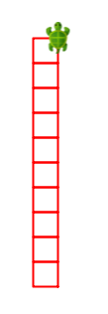
\includegraphics[scale=0.6]{../img/kojo/square-column}

  \columnbreak

  \begin{Code}
  def kvadrat = for (???) {???}
  for (???) {???}
  \end{Code}

  \end{multicols}
  \caption{En kvadratstapel.\label{fig:kojo-lab:column}}
\end{figure}

\Subtask %Kör ditt program med den \emph{gula} play-knappen. 
Studera hur anrop av proceduren \code{kvadrat} påverkar exekveringssekvensen av dina satser genom att göra lämpliga utskrifter så att du kan se när olika delar av koden exekveras. Vid vilka punkter i programmet sker ett ''hopp'' i sekvensen i stället för att efterföljande sats exekveras?  Använd lämpligt argument till \code{sakta} för att du ska hinna studera exekveringen.


\Subtask Rita samma bild med 10 staplade kvadrater (se bild \ref{fig:kojo-lab:column} på sidan \pageref{fig:kojo-lab:column}), men nu \emph{utan} att använda abstraktionen \code{kvadrat} -- använd i stället en nästlad repetition (alltså en upprepning inuti en upprepning). Vilket av de två sätten (med och utan abstraktionen \code{kvadrat}) är lättast att läsa? %\emph{Tips:} Varje gång du trycker på någon av play-knapparna, sparas ditt program. Du kan se dina sparade program om du klickar på \emph{Historik}-fliken. Du kan också stega bakåt och framåt i historiken med de blå pilarna bredvid play-knapparna.

\Subtask Generalisera din abstraktion \code{kvadrat} genom att ge den en parameter \code{sida: Double} som anger hur stor kvadraten blir. Rita flera kvadrater i likhet med bild \ref{fig:kojo-lab:resize} på sidan \pageref{fig:kojo-lab:resize}).

\begin{figure}[H]

\includegraphics{../img/kojo/square-param}
  \caption{Olika stora kvadrater.\label{fig:kojo-lab:resize}}

\end{figure}



%\Subtask\Pen%\Checkpoint
%Se över ditt program i föregående uppgift och säkerställ att det är lättläst och följer en struktur som börjar med alla definitioner i logisk ordning och därefter fortsätter med huvudprogrammet.
%%Diskutera ditt program med en handledare.



%\Subtask\Pen Spara ditt program i en fil men lämpligt namn och ha programmet redo när det är din tur att redovisa vad du gjort under laborationen.
%Anteckna några åtgärder du vidtagit för att göra programmet mer lättläst.







\Task \emph{Alternativ.} \label{kojo:alt}

\Subtask Kör programmet nedan. Förklara vad som händer. %Använd den gula play-knappen för att studera exekveringen.

\begin{Code}
sakta(5000)

def move(key: Int): Unit = {
  println("key: " + key)
  if (key == 87) fram(10)
  else if (key == 83) fram(-10)
}

move(87); move('W'); move('W')
move(83); move('S'); move('S'); move('S')
\end{Code}

\Subtask \label{subtask:keypress}  Kör programmet nedan. Notera \code{activateCanvas} för att du ska slippa klicka i ritfönstret innan du kan styra paddan. Anropet \code{onKeyPress(move)} gör så att \code{move} kommer att anropas då en tangent trycks ned. Lägg till kod i \code{move} som gör att tangenten A ger en vridning moturs med 5 grader medan tangenten D ger en vridning medurs 5 grader. Med \code{onKeyPress} bestämmer man vilken procedur som ska köras vid tangenttryck.

\begin{Code}
sakta(0); activateCanvas

def move(key: Int): Unit = {
  println("key: " + key)
  if (key == 'W') fram(10)
  else if (key == 'S') fram(-10)
}

onKeyPress(move)
\end{Code}



%\Subtask Spara ditt program i en fil men lämpligt namn och ha programmet redo när det är din tur att redovisa vad du gjort under laborationen.


\subsection{Kontrollfrågor}\Checkpoint

\noindent Repetera teorin för denna vecka och var beredd på att kunna svara på dessa frågor när det blir din tur att redovisa vad du gjort under laborationen:

\begin{enumerate}
\item Vad innebär sekventiell exekvering av satser?
\item Vad är skillnaden mellan en sats och ett uttryck?
\item Vad är skillnaden mellan en procedur och en funktion?
\item Spelar ordningen mellan argument någon roll vid anrop av en funktion med flera parametrar?
\item Vad är en variabel? Ge exempel på deklaration, initialisering och tilldelning av variabler, samt användning av variabler i uttryck.
\item Vad är ett logiskt uttryck? Ge exempel på användning av logiska uttryck.
\item Vad är abstraktion? Ge exempel på användning av abstraktion.
\item Vad är nyttan med abstraktion?
\item Vad innebär sidoeffekt? Förklara och ge exempel.
\item Hur deklareras och initialiseras en variabel vars värde är förändringsbart?
\item Hur deklareras och initialiseras en variabel vars värde är oföränderligt?
\item Är det ett körtidsfel eller kompileringsfel att tilldela en oföränderlig variabel ett nytt värde?
\item Ange vilken av \code{for} och \code{while} som är lämpligast i dessa fall:
\begin{itemize}[noitemsep, nolistsep]
\item[A.] Summera de hundra första heltalen.
\item[B.] Räkna antal tecken i en sträng innan första blanktecken.
\item[C.] Dra 100 slumptal mellan 1 och 6 och summera de tal som är mindre än 3.
\item[D.] Summera de första heltalen från 1 och uppåt tills summan är minst 100.
\end{itemize}
\end{enumerate}


\subsection{Frivilliga extrauppgifter}

\noindent Gör i mån intresse och träningsbehov nedan uppgifter i valfri ordning.

\Task \emph{Abstraktion och generalisering}.

\Subtask Skapa en abstraktion \code{def stapel = ???} som använder din abstraktion \code{kvadrat}.

\Subtask Du ska nu \emph{generalisera} din procedur så att den inte bara kan rita exakt 10 kvadrater i en stapel. Ge proceduren \code{stapel} en parameter \code{n} som styr hur många kvadrater som ritas.
\begin{Code}
def kvadrat = ???
def stapel(n: Int) = ???

sakta(100)
stapel(42)
\end{Code}



\Subtask Rita nedan bild med hjälp av abstraktionen \code{stapel}. Det är totalt 100 kvadrater och varje kvadrat har sidan 25. \emph{Tips:} Med ett negativt argument till procedur \code{hoppa} kan du få sköldpaddan att hoppa baklänges utan att rita, t.ex. \code{hoppa(-10*25)}

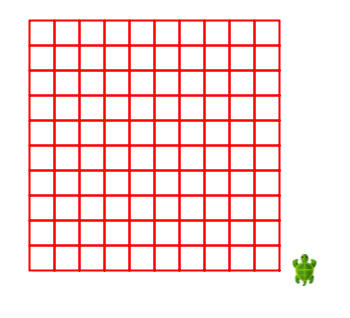
\includegraphics[width=0.3\textwidth]{../img/kojo/square-grid}

\Subtask Generalisera dina abstraktioner \code{kvadrat} och \code{stapel} så att man kan påverka storleken på kvadraterna som ritas ut.

\Subtask Skapa en abstraktion \code{rutnät} med lämpliga parametrar som gör att man kan rita rutnät med olika stora kvadrater och olika många kvadrater i både x- och y-led.

\Subtask Generalisera dina abstraktioner \code{kvadrat} och \code{stapel} så att man kan påverka fyllfärgen och pennfärgen för kvadraterna som ritas ut.

\Task \emph{Växling med booleska värden.}

\Subtask Bygg vidare på programmet i uppgift \ref{kojo:alt} och lägg till nedan kod i början av programmet. Lägg även till kod som gör så att om man trycker på tangenten G så sätts rutnätet omväxlande på och av. Observera att det är exakt \emph{en} procedur som anropas vid \code{onKeyPress}.

\begin{Code}
var isGridOn = false

def toggleGrid =
  if (isGridOn) {
    gridOff
    isGridOn = false
  } else {
    gridOn
    isGridOn = true
  }
\end{Code}

\Subtask Gör så att när man trycker på tangenten X så sätter man omväxlande på och av koordinataxlarna. Använd en variabel \code{isAxesOn} och definiera en abstraktion \code{toggleAxes} som anropar \code{axesOn} och \code{axesOff} på liknande sätt som i föregående uppgift.


\Task \emph{Repetition.}~Skriv en procedur \code{randomWalk} med detta huvud: \\
\code{def randomWalk(n: Int, maxStep: Int, maxAngle: Int): Unit}\\ som gör så att paddan tar \code{n} steg av slumpmässig längd mellan \code{0} och \code{maxStep}, samt efter varje steg vrider sig åt vänster en slumpmässig vinkel mellan \code{0} och \code{maxAngle}. Anropa din procedur med olika argument och undersök hur dess värden påverkar bildens utseende. \emph{Tips:} Uttrycket \code{math.random() * 100} ger ett tal från 0 till (nästan) 100. Du kan styra hur långsamt paddan ritar genom anrop av \code{sakta(???)} (prova dig fram till något  lämpligt heltalsargument i stället för \code{???}).
\vspace{2em}\\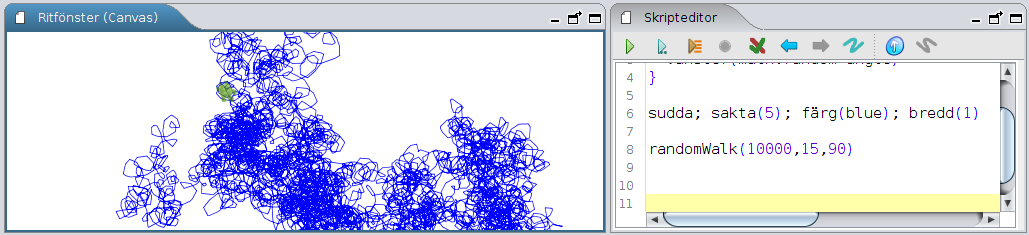
\includegraphics[width=\textwidth]{../img/kojo/random-walk.png}


\Task \emph{Variabler, namngivning och formatering.}

\Subtask Klistra in nedan konstigt formatterade program \emph{exakt} som det står med blanktecken, indragningar och radbrytningar. Kör programmet och förklara vad som händer.

\begin{figure}[H]
\begin{Code}
// Ett konstigt formaterat program med en del konstiga namn.

def gurka(x: Double,
y: Double, namn: String,
typ: String,
värde:String) = {
val tomat = 15
val h = 30
hoppaTill(x,y)
norr
skriv(namn+": "+typ)
hoppaTill(x+tomat*(namn.size+typ.size),y)
skriv(värde); söder; fram(h); vänster
fram(tomat * värde.size); vänster
fram(h); vänster
fram(tomat * värde.size); vänster }
sudda; färg(svart); val s = 130
val h = 40
var x = 42; gurka(10, s-h*0, "x","Int", x.toString)
var y = x; gurka(10, s-h*1, "y","Int", y.toString)
x = x + 1; gurka(10, s-h*2, "x","Int", x.toString)
gurka(10, s-h*3, "y","Int", y.toString); osynlig
\end{Code}
\end{figure}

\Subtask\Pen Skriv ner namnet på alla variabler som förekommer i programmet.

\Subtask\Pen Vilka av dessa variabler är lokala?

\Subtask\Pen Vilka av dessa variabler kan förändras efter initialisering?

\Subtask\Pen Föreslå tre förändringar av programmet ovan (till exempel namnbyten) som gör att det blir lättare att läsa och förstå.

\Subtask Gör sök-ersätt av \code{gurka} till ett bättre namn. \emph{Tips:} undersök kontextmenyn i editorn i Kojo genom att högerklicka. Använd kortkommandot för Sök/Ersätt.

\Subtask Gör automatisk formatering av koden med hjälp av lämpligt kortkommando. Notera skillnaderna. Vilka autoformateringar gör programmet lättare att läsa? Vilka manuella formateringar tycker du bör göras för att öka läsbarheten? Ge funktionen \code{gurka} ett bättre namn.  Diskutera läsbarheten med en handledare.



\Task \label{task:measuretime} \emph{Tidmätning.} Hur snabb är din dator?

\Subtask \label{task:timer} Skriv in koden nedan i Kojos editor och kör upprepade gånger med den gröna play-knappen. Tar det lika lång tid varje gång? Varför?

\begin{Code}
object timer {
  def now: Long = System.currentTimeMillis
  var saved: Long = now
  def elapsedMillis: Long = now - saved
  def elapsedSeconds: Double = elapsedMillis / 1000.0
  def reset: Unit = { saved = now }
}

// HUVUDPROGRAM:
timer.reset
var i = 0L
while (i < 1e8.toLong) { i += 1 }
val t = timer.elapsedSeconds
println("Räknade till " + i + " på " + t + " sekunder.")
\end{Code}


\Subtask Ändra i loopen i uppgift \ref{task:timer}) så att den räknar till 4.4 miljarder. Hur lång tid tar det för din dator att räkna så långt?\footnote{Det går att göra ungefär en heltalsaddition per klockcykel per kärna. Den första elektroniska datorn \href{https://sv.wikipedia.org/wiki/ENIAC}{Eniac} hade en klockfrekvens motsvarande 5 kHz. Den dator på vilken denna övningsuppgift skapades hade en i7-4790K turboklockad upp till 4.4 GHz.
%\href{http://www.extremetech.com/computing/185512-overclocking-intels-core-i7-4790k-can-devils-canyon-fix-haswells-low-clock-speeds/2}{www.extremetech.com/computing/185512-overclocking-intels-core-i7-4790k-can-devils-canyon-fix-haswells-low-clock-speeds/2}
}

\Subtask  Om du kör på en Linux-maskin: Kör nedan Linux-kommando upprepade gånger i ett terminalfönster. Med hur många MHz kör din dators klocka för tillfället? Hur förhåller sig klockfrekvensen till antalet rundor i while-loopen i föregående uppgift? (Det kan hända att din dator kan variera centralprocessorns klockfrekvens. Prova både medan du kör tidmätningen i Kojo och då din dator ''vilar''. Vad är det för poäng med att en processor kan variera sin klockfrekvens?)
\begin{REPLnonum}
> lscpu | grep MHz
\end{REPLnonum}


\Subtask Ändra i koden i uppgift \ref{task:timer}) så att \code{while}-loopen bara kör 5 gånger. %Kör programmet med den \emph{gula} play-knappen. Scrolla i programspårningen och förklara vad som händer. Klicka på \code{CALL}-rutorna och se vilken rad som markeras i ditt program.

\Subtask Lägg till koden nedan i ditt program och försök ta reda på ungefär hur långt din dator hinner räkna till på en sekund för \code{Long}- respektive \code{Int}-variabler. Använd den gröna play-knappen.
\begin{CodeSmall}
def timeLong(n: Long): Double = {
  timer.reset
  var i = 0L
  while (i < n) { i += 1 }
  timer.elapsedSeconds
}

def timeInt(n: Int): Double = {
  timer.reset
  var i = 0
  while (i < n) { i += 1 }
  timer.elapsedSeconds
}

def show(msg: String, sec: Double): Unit = {
  print(msg + ": ")
  println(sec + " seconds")
}

def report(n: Long): Unit = {
  show("Long " + n, timeLong(n))
  if (n <= Int.MaxValue) show("Int  " + n, timeInt(n.toInt))
}

// HUVUDPROGRAM, mätningar:

report(Int.MaxValue)
for (i <- 1 to 10) report(4.26e9.toLong)
\end{CodeSmall}

\Subtask Hur mycket snabbare går det att räkna med \code{Int}-variabler jämfört med \code{Long}-variabler? Diskutera gärna svaret med en handledare.

\Task Lek med färg i Kojo. Sök på internet efter dokumentationen för klassen \code{java.awt.Color} och studera vilka heltalsparametrar den sista konstruktorn i listan med konstruktorer tar för att skapa sRGB-färger. Om du högerklickar i editorn i Kojo och väljer ''Välj färg...'' får du fram färgväljaren och med den kan du välja fördefinierade färger eller blanda egna färger. När du har valt färg får du se vilka parametrar till \code{java.awt.Color} som skapar färgen. Testa detta i REPL:

\begin{REPL}
scala> val c = new java.awt.Color(124,10,78,100)
c: java.awt.Color = java.awt.Color[r=124,g=10,b=78]

scala> c.  // tryck på TAB
asInstanceOf    getColorComponents      getRGBComponents
brighter        getColorSpace           getRed
createContext   getComponents           getTransparency
darker          getGreen                isInstanceOf
getAlpha        getRGB                  toString
getBlue         getRGBColorComponents

scala> c.getAlpha
res3: Int = 100
\end{REPL}
Skriv ett program som ritar många figurer med olika färger, till exempel cirklar som nedan. Om du använder alfakanalen blir färgerna genomskinliga.

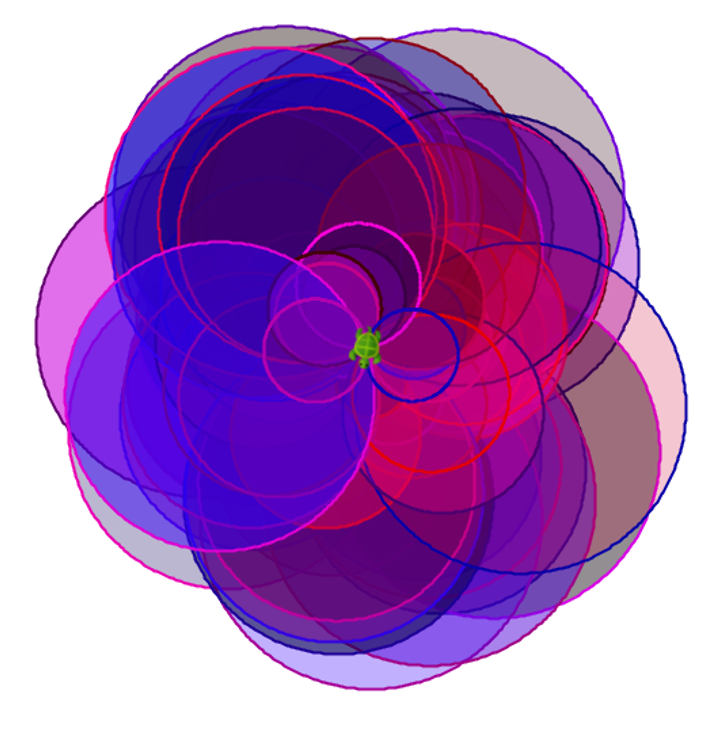
\includegraphics[width=0.82\textwidth]{../img/kojo/random-color-circles.png}


\Task Ladda ner ''Uppdrag med Kojo'' från \href{http://lth.se/programmera/uppdrag}{lth.se/programmera/uppdrag}  och gör några uppgifter som du tycker verkar intressanta.

%\Subtask ''Programming Fundamentals with Kojo'' som kan laddas ner här:\\
%\href{http://wiki.kogics.net/kojo-codeactive-books}{wiki.kogics.net/kojo-codeactive-books}

\Task Om du vill jobba med att hjälpa skolbarn att lära sig programmera med Kojo, kontakta \url{http://www.vattenhallen.lth.se} och anmäl ditt intresse att vara handledare.


\chapter{Kodstrukturer}\label{chapter:W02}
\begin{itemize}[nosep]
\item samling: Range
\item for-uttryck
\item map
\item foreach
\item flatMap
\item algoritm vs implementation
\item pseudokod
\item algoritm: swap
\item algoritm: summering
\item algoritm: min/max
\item paket
\item import
\item filstruktur
\item jar
\item dokumentation
\item programlayout
\item JDK
\item konstanter vs föränderlighet
\item objektorientering
\item klasser
\item objekt
\item punktnotation
\item referensvariabler
\item referenstilldelning
\item anropa metoder
\item block
\item namnsynlighet
\item namnöverskuggning
\item SimpleWindow
\end{itemize}

%!TEX encoding = UTF-8 Unicode
%!TEX root = ../exercises.tex

\ifPreSolution

\Exercise{\ExeWeekTWO}\label{exe:W02}
\begin{Goals}
%!TEX encoding = UTF-8 Unicode
%!TEX root = ../compendium2.tex

\item Kunna skapa samlingarna Range, Array och Vector med heltals- och strängvärden.
\item Kunna indexera i en indexerbar samling, t.ex. Array och Vector.
\item Kunna anropa operationerna size, mkString, sum, min, max på samlingar som innehåller heltal.
\item Känna till grundläggande skillnader och likheter mellan samlingarna Range, Array och Vector.
\item Förstå skillnaden mellan en for-sats och ett for-uttryck.
\item Kunna skapa samlingar med heltalsvärden som resultat av enkla for-uttryck.
\item Förstå skillnaden mellan en algoritm i pseudo-kod och dess implementation.
\item Kunna implementera algoritmerna SUM, MIN/MAX på en indexerbar samling med en \code{while}-sats.
\item Kunna köra igång enkel Scala-kod i REPL, som skript och som applikation.
\item Kunna skriva och köra igång ett enkelt Java-program.
\item Känna till några grundläggande syntaxskillnader mellan Scala och Java, speciellt variabeldeklarationer och indexering i Array.
\item Förstå vad ett block och en lokal variabel är.
\item Förstå hur nästlade block påverkar namnsynlighet och namnöverskuggning.
\item Förstå kopplingen mellan paketstruktur och kodfilstruktur.
\item Kunna skapa en jar-fil.
\item Kunna skapa dokumentation med scaladoc.

\end{Goals}

\begin{Preparations}
\item \StudyTheory{02}
\item Bekanta dig med grundläggande terminalkommandon, se appendix~\ref{appendix:terminal}.
\item Bekanta dig med den editor du vill använda, se appendix~\ref{appendix:compile}.
\end{Preparations}

\else

\ExerciseSolution{\ExeWeekTWO}

\fi


% TODO fundera på detta:
% terminalkommando
% scalac -> hello world; scala som script; javac
% paket, import, jar, main,



\BasicTasksNoLab %%%%%%%%%%%%%%%%




\WHAT{Para ihop begrepp med beskrivning.}

\QUESTBEGIN

\Task \what

\vspace{1em}\noindent Koppla varje begrepp med den (förenklade) beskrivning som passar bäst:

\begin{ConceptConnections}
  kompilerad & 1 & & A & datastruktur med element av samma typ \\ 
  skript & 2 & & B & en oföränderlig, indexerbar sekvenssamling \\ 
  objekt & 3 & & C & en specifik realisering av en algoritm \\ 
  main & 4 & & D & maskinkod sparas ej utan skapas vid varje körning \\ 
  programargument & 5 & & E & applicerar en funktion på varje element i en samling \\ 
  datastruktur & 6 & & F & datastruktur med element i en viss ordning \\ 
  samling & 7 & & G & där exekveringen av kompilerad app startar \\ 
  sekvenssamling & 8 & & H & maskinkod sparad och kan köras igen utan kompilering \\ 
  Array & 9 & & I & en förändringsbar, indexerbar sekvenssamling \\ 
  Vector & 10 & & J & stegvis beskrivning av en lösning på ett problem \\ 
  Range & 11 & & K & en samling som representerar ett intervall av heltal \\ 
  yield & 12 & & L & samlar variabler och funktioner \\ 
  map & 13 & & M & många olika element i en helhet; elementvis åtkomst \\ 
  algoritm & 14 & & N & överförs via parametern args i main \\ 
  implementation & 15 & & O & används i for-uttryck för att skapa ny samling \\ 
\end{ConceptConnections}

\SOLUTION

\TaskSolved \what

\begin{ConceptConnections}
  kompilerad & 1 & ~~\Large$\leadsto$~~ &  L & maskinkod sparad och kan köras igen utan kompilering \\ 
  skript & 2 & ~~\Large$\leadsto$~~ &  F & maskinkod sparas ej utan skapas vid varje körning \\ 
  objekt & 3 & ~~\Large$\leadsto$~~ &  N & samlar variabler och funktioner \\ 
  main & 4 & ~~\Large$\leadsto$~~ &  G & där exekveringen av kompilerad app startar \\ 
  programargument & 5 & ~~\Large$\leadsto$~~ &  I & överförs via parametern args i main \\ 
  datastruktur & 6 & ~~\Large$\leadsto$~~ &  E & många olika element i en helhet; elementvis åtkomst \\ 
  samling & 7 & ~~\Large$\leadsto$~~ &  O & datastruktur med element av samma typ \\ 
  sekvenssamling & 8 & ~~\Large$\leadsto$~~ &  K & datastruktur med element i en viss ordning \\ 
  Array & 9 & ~~\Large$\leadsto$~~ &  B & en förändringsbar, indexerbar sekvenssamling \\ 
  Vector & 10 & ~~\Large$\leadsto$~~ &  D & en oföränderlig, indexerbar sekvenssamling \\ 
  Range & 11 & ~~\Large$\leadsto$~~ &  J & en samling som representerar ett intervall av heltal \\ 
  yield & 12 & ~~\Large$\leadsto$~~ &  C & används i for-uttryck för att skapa ny samling \\ 
  map & 13 & ~~\Large$\leadsto$~~ &  A & applicerar en funktion på varje element i en samling \\ 
  algoritm & 14 & ~~\Large$\leadsto$~~ &  M & stegvis beskrivning av en lösning på ett problem \\ 
  implementation & 15 & ~~\Large$\leadsto$~~ &  H & en specifik realisering av en algoritm \\ 
\end{ConceptConnections}

\QUESTEND





\WHAT{Använda terminalen.}

\QUESTBEGIN

\Task \what~Läs om terminalen i appendix \ref{appendix:terminal}.

\Subtask Vilka tre kommando ska du köra för att 1) skapa en katalog med namnet \code{hello} och 2)  navigera till katalogen och 3) visa namnet på ut aktuell katalog? Öppna ett teminalfönster och kör dessa tre kommando.

\Subtask Vilka två kommando ska du köra för att 1) navigera tillbaka ''upp'' ett steg i filträdet och 2) lista alla filer och kataloger på denna plats? Kör dessa två kommando i terminalen.

\SOLUTION

\TaskSolved \what

\SubtaskSolved

\begin{REPL}
> mkdir hello
> cd hello
> pwd
\end{REPL}

\SubtaskSolved

\begin{REPL}
> cd ..
> ls
\end{REPL}


\QUESTEND









\WHAT{Skapa och köra ett Scala-skript.}

\QUESTBEGIN

\Task  \what~

\Subtask Skapa en fil med namn \texttt{sum.scala} i katalogen \code{hello} som du skapade i föregående uppgift med hjälp av en editor, t.ex. \code{atom}.
\begin{REPLnonum}
> cd hello
> atom sum.scala
\end{REPLnonum}

\noindent Filen ska innehålla dessa tre rader:
\scalainputlisting{examples/sum.scala}

\noindent Spara filen och kör kommandot \code{scala sum.scala} i terminalen:
\begin{REPLnonum}
> scala sum.scala
\end{REPLnonum}

\noindent Vad blir summan av de $1000$ första talen?

\Subtask Ändra i filen \code{sum.scala} så att högerparentesen på sista raden saknas. Spara filen (Ctrl+S) och kör skriptfilen igen i terminalen (pil-upp). Hur lyder felmeddelandet? Är det ett körtidsfel eller ett kompileringsfel?

\Subtask Ändra i hello-script.scala så att det i stället för \code{1000} står \code{args(0).toInt} efter \code{val n =} och spara och kör om ditt program med argumentet 5001 så här:
\begin{REPL}
> scala hello-script.scala 5001
\end{REPL}
\noindent Vad blir summan av de $5001$ första talen?

\Subtask Vad blir det för felmeddelande om du glömmer ge programmet ett argument? Är det ett körtidsfel eller ett kompileringsfel?

\SOLUTION

\TaskSolved \what

\SubtaskSolved
\begin{REPL}
Summan av de 1000 första talen är: 500500
\end{REPL}

\SubtaskSolved  Kompileringsfelet blir: \code{error: ')' expected but eof found}

\SubtaskSolved  Filen ska se ut så här:
\begin{Code}
val n = args(0).toInt
val summa = (1 to n).sum
println(s"Summan av de $n första talen är: $summa")
\end{Code}

Utskriften blir så här:
\begin{REPL}
Summan av de 5001 första talen är: 12507501
\end{REPL}

\SubtaskSolved Körtidsfelet blir: \code{java.lang.ArrayIndexOutOfBoundsException: 0}\\(Anledningen är att arrayen \code{args} blir tom om programargument saknas och platsen med index $0$ därmed inte finns.)

\QUESTEND





\WHAT{Scala-applikation med \code+main+-metod.}

\QUESTBEGIN

\Task  \what~  Skapa med hjälp av en editor en fil med namn \texttt{hello.scala}.
\begin{REPLnonum}
> atom hello.scala
\end{REPLnonum}
Skriv nedan kod i filen:


\scalainputlisting{examples/hello.scala}

\Subtask Kompilera med \code{scalac hello.scala} och kör koden med \code{scala Hello}. Notera stor bokstav i klassnamnet. Vad heter filerna som kompilatorn skapar?
\begin{REPLnonum}
> scalac hello.scala
> ls
> scala Hello
\end{REPLnonum}

\Subtask Hur ska du ändra i din kod så att kompilatorn ger följande felmeddelande: \\
\texttt{Missing closing brace}

\Subtask Varför behövs \code{main}-metoden?

\Subtask Vilket alternativ går snabbast att köra igång, ett skript eller en kompilerad applikation? Varför? Vilket alternativ kör snabbast när väl exekveringen är igång?


\SOLUTION


\TaskSolved \what


\SubtaskSolved  Filerna som kompilatorn skapat heter \code{Hello.class} och \verb+Hello\$.class+

\SubtaskSolved  Felmeddelandet får du om du tar bort den sista krullparentesen.

\SubtaskSolved

\begin{itemize}
  \item  Det går snabbare att göra i gång en kompilerad app eftersom maskinkoden är sparad i en fil som kan köras igång direkt. En kompilerad app måste ha ett objekt med en main-metod. En kompilerad app kan bestå av många filer som samkompileras.
  \item När ett skript kör kompileras koden i skriptfilen före varje körning och maskinkoden sparas inte. Ett skript består bara av en enda text-fil som körs från början. Ingen main-metod behövs.
  \item  När väl exekveringen är igång sker exekveringen av maskinkoden exakt lika snabbt oberoende av om koden är genererad ur ett skript eller en förkompilerad app.
\end{itemize}

\QUESTEND







\WHAT{Java-applikation.}

\QUESTBEGIN

\Task \label{task:java} \what~   Skapa med hjälp av en editor en fil med namn \texttt{Hi.java}. Notera stor bokstav. I ett Java-program måste namnet före \code{.java} stämma överens exakt med klassnamnet.
\begin{REPLnonum}
> atom Hi.java
\end{REPLnonum}
Skriv dessa rader i filen:
\javainputlisting{examples/Hi.java}
\noindent Kompilera med \code{javac Hi.java} och kör koden med \code{java Hi}.
\begin{REPLnonum}
> javac Hi.java
> ls
> java Hi
\end{REPLnonum}

\Subtask Vad heter filen som kompilatorn skapat?

\Subtask Jämför Java-programmet ovan med Scala-programmet i föregående uppgift. Programmen gör samma sak men syntaxen (hur koden ska skrivas) skiljer sig åt och det finns vissa skillnader i semantiken (vad koden betyder). Vi ska senare i kursen gå igenom \emph{exakt} vad varje fragment nedan betyder, men försök redan nu para ihop de Scala-delar till vänster som (ungefär) motsvarar de Java-delar som finns till höger.

\begin{ConceptConnections}
  \code|object| & 1 & & A & \jcode|public static main| \\ 
  \code|def main| & 2 & & B & \jcode|public class| \\ 
  \code|Array[String]| & 3 & & C & \jcode|void| \\ 
  \code|: Unit| & 4 & & D & \jcode|) {| \\ 
  \code|=| & 5 & & E & \jcode|System.out.println| \\ 
  \code|println| & 6 & & F & \jcode|String[]| \\ 
\end{ConceptConnections}

\SOLUTION


\TaskSolved \what


\SubtaskSolved  Hi.class

\SubtaskSolved

\begin{ConceptConnections}
  \code|object| & 1 & ~~\Large$\leadsto$~~ &  E & \jcode|public class| \\ 
  \code|def main| & 2 & ~~\Large$\leadsto$~~ &  B & \jcode|public static main| \\ 
  \code|Array[String]| & 3 & ~~\Large$\leadsto$~~ &  F & \jcode|String[]| \\ 
  \code|: Unit| & 4 & ~~\Large$\leadsto$~~ &  A & \jcode|void| \\ 
  \code|=| & 5 & ~~\Large$\leadsto$~~ &  D & \jcode|) {| \\ 
  \code|println| & 6 & ~~\Large$\leadsto$~~ &  C & \jcode|System.out.println| \\ 
\end{ConceptConnections}


\QUESTEND




\WHAT{Skapa och använda samlingar.}

\QUESTBEGIN

\Task \what~I Scalas standardbibliotek finns många olika samlingar som går att använda på ett enhetligt sätt (med vissa undantag för \code{Array}). Para ihop uttrycken som skapar eller använder samlingar med förklaringarna, så att alla kopplingar blir korrekta (minst en förklaring passar med mer än ett uttryck, men det finns bara en lösning där alla kopplingar blir parvis korrekta):

\begin{ConceptConnections}
  \code|val xs = Vector(2) | & 1 & & A & ny samling med en nolla tillagd i början \\ 
  \code|Array.fill(9)(0)   | & 2 & & B & ny samling med en nolla tillagd på slutet \\ 
  \code|Vector.fill(9)(' ')| & 3 & & C & förkortad skrivning av \code|apply(0)| \\ 
  \code|xs(0)              | & 4 & & D & ny förändringsbar sekvens med nollor \\ 
  \code|xs.apply(0)        | & 5 & & E & ny samling, elementen omgjorda till heltal \\ 
  \code|xs :+ 0            | & 6 & & F & ny samling, elementen omgjorda till strängar \\ 
  \code|0 +: xs            | & 7 & & G & ny sträng med alla element intill varandra \\ 
  \code|xs.mkString        | & 8 & & H & ny sträng med komma mellan elementen \\ 
  \code|xs.mkString(",") | & 9 & & I & indexering, ger första elementet \\ 
  \code|xs.map(_.toString) | & 10 & & J & ny oföränderlig sekvens med blanktecken \\ 
  \code|xs map (_.toInt)   | & 11 & & K & ny referens till sekvens av längd 1 \\ 
\end{ConceptConnections}

\noindent Träna med dina egna varianter i REPL tills du lärt dig använda uttryck som ovan utantill. Då har du lättare att komma igång med kommande laborationer.

\SOLUTION

\TaskSolved \what

\begin{ConceptConnections}
  \code|val xs = Vector(2) | & 1 & ~~\Large$\leadsto$~~ &  J & ny referens till sekvens av längd 1 \\ 
  \code|Array.fill(9)(0)   | & 2 & ~~\Large$\leadsto$~~ &  E & ny förändringsbar sekvens med nollor \\ 
  \code|Vector.fill(9)(' ')| & 3 & ~~\Large$\leadsto$~~ &  D & ny oföränderlig sekvens med blanktecken \\ 
  \code|xs(0)              | & 4 & ~~\Large$\leadsto$~~ &  C & förkortad skrivning av \code|apply(0)| \\ 
  \code|xs.apply(0)        | & 5 & ~~\Large$\leadsto$~~ &  H & indexering, ger första elementet \\ 
  \code|xs :+ 0            | & 6 & ~~\Large$\leadsto$~~ &  B & ny samling med en nolla tillagd på slutet \\ 
  \code|0 +: xs            | & 7 & ~~\Large$\leadsto$~~ &  F & ny samling med en nolla tillagd i början \\ 
  \code|xs.mkString        | & 8 & ~~\Large$\leadsto$~~ &  A & ny sträng med alla element intill varandra \\ 
  \code|xs.mkString(",") | & 9 & ~~\Large$\leadsto$~~ &  G & ny sträng med komma mellan elementen \\ 
  \code|xs.map(_.toString) | & 10 & ~~\Large$\leadsto$~~ &  K & ny samling, elementen omgjorda till strängar \\ 
  \code|xs map (_.toInt)   | & 11 & ~~\Large$\leadsto$~~ &  I & ny samling, elementen omgjorda till heltal \\ 
\end{ConceptConnections}

\QUESTEND





\WHAT{Jämför \code{Array} och \code{Vector}.}

\QUESTBEGIN

\Task \what~Para ihop varje samlingstyp med den beskrivning som passar bäst:

\Subtask Föränderlighet \Eng{mutability}.

\begin{ConceptConnections}
  Vector & 1 & & A & förändringsbar \\ 
  Array & 2 & & B & oföränderlig \\ 
\end{ConceptConnections}

\Subtask Tillägg av element i början \Eng{prepend} och slutet \Eng{append}, eller förändring av delsekvens på godtycklig plats (eng. \emph{to patch}, även på svenska: \emph{att patcha}).

\begin{ConceptConnections}
  Vector & 1 & & A & långsam vid ändring av storlek (kopiering av rubbet krävs) \\ 
  Array & 2 & & B & varianter med fler/andra element skapas snabbt ur befintlig \\ 
\end{ConceptConnections}

\Subtask Likhet \Eng{equality}.

\begin{ConceptConnections}
  Vector & 1 & & A & olikt andra Scala-samlingar kollar \code|==| ej innehållslikhet \\ 
  Array & 2 & & B & \code|xs == ys| är \code|true| om alla element lika \\ 
\end{ConceptConnections}


\SOLUTION

\TaskSolved \what

\Subtask

\begin{ConceptConnections}
  Vector & 1 & ~~\Large$\leadsto$~~ &  A & oföränderlig \\ 
  Array & 2 & ~~\Large$\leadsto$~~ &  B & förändringsbar \\ 
\end{ConceptConnections}

\Subtask

\begin{ConceptConnections}
  Vector & 1 & ~~\Large$\leadsto$~~ &  B & varianter med fler/andra element skapas snabbt ur befintlig \\ 
  Array & 2 & ~~\Large$\leadsto$~~ &  A & långsam vid ändring av storlek (kopiering av rubbet krävs) \\ 
\end{ConceptConnections}

\Subtask

\begin{ConceptConnections}
  Vector & 1 & ~~\Large$\leadsto$~~ &  B & \code|xs == ys| är \code|true| om alla element lika \\ 
  Array & 2 & ~~\Large$\leadsto$~~ &  A & olikt andra samlingar kollar \code|==| ej innehållslikhet \\ 
\end{ConceptConnections}

\QUESTEND







\WHAT{Räkna ut summa, min och max i \code{args}.}

\QUESTBEGIN

\Task \what~Skriv ett program som skriver ut summa, min och max för en sekvens av heltal i \code{args}. Du kan förutsätta att programmet bara körs med heltal som programparametrar. \emph{Tips:} Med uttrycken \code{xs.sum} och \code{xs.min} och \code{xs.max} ges summan, minsta resp. största värde.
%Med uttrycket \code{xs.map(_.toInt)} ges en ny samling med alla element omgjorda till heltal.

Exempel på körning i terminalen:
\begin{REPL}
> atom sum-min-max.scala
> scalac sum-min-max.scala
> scala SumMinMax 1 2 42 3 4
52 1 42
\end{REPL}

\SOLUTION

\TaskSolved \what~

\scalainputlisting{examples/sum-min-max.scala}

\QUESTEND






\WHAT{Algoritm: SWAP.}

\QUESTBEGIN

\Task  \what~\\\emph{Problem:} Byta plats på två variablers värden. \\\emph{Lösningsidé:} Använd temporär variabel för mellanlagring.

\Subtask Skriv med \emph{pseudo-kod} (steg för steg på vanlig svenska) algoritmen SWAP nedan.

\emph{Indata:} två heltalsvariabler $x$ och $y$

\textbf{???}

\emph{Utdata:} variablerna $x$ och $y$ vars värden har bytt plats.

\Subtask Implementerar algoritmen SWAP. Ersätt \code{???} nedan med kod som byter plats på värdena i variablerna \code{x} och \code{y}:

\begin{REPL}
scala> var x = 42; var y = 43
scala> ???
scala> println("x är " + x + ", y är " + y)
x är 43, y är 42
\end{REPL}

\SOLUTION

\TaskSolved \what

\SubtaskSolved  Pseudokoden kan se ut såhär:
\begin{Code}
Deklarera heltalsvariabel temp.
Kopiera värdet från x till temp.
Kopiera värdet från y till x.
Kopiera värdet från temp till y.
\end{Code}

\SubtaskSolved
\begin{Code}
var temp = x
x = y
y = temp
\end{Code}

\QUESTEND




\WHAT{Indexering och tilldelning i Array med SWAP.}

\QUESTBEGIN

\Task \what~Skriva ett program som byter plats på första och sista elementet i \code{main}-parametern \code{args}. Bytet ska bara ske om det är minst två element i \code{args}. Oavsett om förändring skedde eller ej ska \code{args} sedan skrivas ut med blanktecken mellan argumenten.
  \emph{Tips:} Du kan komma åt sista elementet med \code{args(args.size - 1)}

Exempel på körning i terminalen:
\begin{REPL}
> atom swap-args.scala
> scalac swap-args.scala
> scala SwapFirstLastArg hej alla barn
barn alla hej
\end{REPL}

\SOLUTION

\TaskSolved \what~

\scalainputlisting{examples/swap-args.scala}

\QUESTEND



\WHAT{\code|for|-uttryck och \code|map|-uttryck.}

\QUESTBEGIN

\Task \what~Variabeln \code{xs} nedan refererar till samlingen \code{Vector(1, 2, 3)}. Para ihop uttrycken till vänster med rätt värde till höger.

\begin{ConceptConnections}
  \code|for (x <- xs) yield x * 2| & 1 & & A & \code|Vector(2, 3, 4)| \\ 
  \code|for (i <- xs.indices) yield i| & 2 & & B & \code|Vector(2, 4, 6)| \\ 
  \code|xs.map(x => x + 1)    | & 3 & & C & \code|Vector(0, 1, 2)| \\ 
  \code|for (i <- 0 to 1) yield xs(i)| & 4 & & D & \code|Vector(1, 2)| \\ 
  \code|(1 to 3).map(i => i)| & 5 & & E & \code|Vector(1, 2, 3)| \\ 
  \code|(1 until 3).map(i => xs(i))| & 6 & & F & \code|Vector(2, 3)| \\ 
\end{ConceptConnections}

\noindent Träna med dina egna varianter i REPL tills du lärt dig använda uttryck som ovan utantill. Då har du lättare att komma igång med kommande laborationer.

\SOLUTION

\TaskSolved \what

\begin{ConceptConnections}
  \code|for (x <- xs) yield x * 2| & 1 & ~~\Large$\leadsto$~~ &  F & \code|Vector(1, 2, 4)| \\ 
  \code|for (i <- xs.indices) yield i| & 2 & ~~\Large$\leadsto$~~ &  C & \code|Vector(0, 1, 2)| \\ 
  \code|xs.map(x => x + 1)    | & 3 & ~~\Large$\leadsto$~~ &  D & \code|Vector(2, 3, 4)| \\ 
  \code|for (i <- 0 to 1) yield xs(i)| & 4 & ~~\Large$\leadsto$~~ &  B & \code|Vector(1, 2)| \\ 
  \code|(1 to 3).map(i => i)| & 5 & ~~\Large$\leadsto$~~ &  A & \code|Vector(1, 2, 3)| \\ 
  \code|(1 until 3).map(i => xs(i))| & 6 & ~~\Large$\leadsto$~~ &  E & \code|Vector(2, 3)| \\ 
\end{ConceptConnections}

\QUESTEND






\WHAT{Algoritm: SUMBUG}

\QUESTBEGIN

\Task  \what~ . Nedan återfinns pseudo-koden för SUMBUG.

\begin{algorithm}[H]
 \SetKwInOut{Input}{Indata}\SetKwInOut{Output}{Resultat}

 \Input{heltalet $n$}
 \Output{utskrift av summan av de första $n$ heltalen }
 $sum \leftarrow 0$ \\
 $i \leftarrow 1$  \\
 \While{$i \leq n$}{
  $sum \leftarrow sum + 1$
 }
 skriv ut $sum$
\end{algorithm}

\Subtask Kör algoritmen steg för steg med penna och papper, där du skriver upp hur värdena för respektive variabel ändras. Det finns två buggar i algoritmen. Vilka? Rätta buggarna och test igen genom att ''köra'' algoritmen med penna på papper och kontrollera så att algoritmen fungerar för $n=0$, $n=1$, och $n=5$. Vad händer om $n=-1$?

\Subtask Skapa med hjälp av en editor filen \code{sumn.scala}. Implementera algoritmen SUM enligt den rättade pseudokoden och placera implementationen i en main-metod i ett objekt med namnet \code{sumn}. Du kan skapa indata \code{n} till algoritmen med denna deklaration i början av din main-metod: \\ \code{val n = args(0).toInt} \\ Vad ger applikationen för utskrift om du kör den med argumentet 8888?

\begin{REPLnonum}
> scalac sumn.scala
> scala sumn 8888
\end{REPLnonum}

\noindent Kontrollera att din implementation räknar rätt genom att jämföra svaret med detta uttrycks värde, evaluerat i Scala REPL:
\begin{REPLnonum}
scala> (1 to 8888).sum
\end{REPLnonum}

\Subtask Implementera algoritmen SUM enligt pseudokoden ovan, men nu i Java. Skapa filen \code{SumN.java} och använd koden från uppgift \ref{task:java} som mall för att deklarera den publika klassen \code{SumN} med en main-metod. Några tips om Java-syntax och standarfunktioner i Java:

\begin{itemize}[noitemsep, nolistsep]
\item Alla satser i Java måste avslutas med semikolon.
\item Heltalsvariabler deklareras med nyckelordet \lstinline[language=Java]{int} (litet i).
\item Typnamnet ska stå \emph{före} namnet på variabeln. Exempel: \\ \lstinline[language=Java]{int sum = 0;}
\item Indexering i en array görs i Java med hakparenteser: \code{args[0]}
\item I stället för Scala-uttrycket \code{args(0).toInt}, använd Java-uttrycket: \\ \code{Integer.parseInt(args[0])}
\item \code{while}-satser i Scala och Java har samma syntax.
\item Utskrift i Java görs med \code{System.out.println}
\end{itemize}


\SOLUTION


\TaskSolved \what


\SubtaskSolved  Bugg: Eftersom \code{i} inte inkrementeras, fastnar programmet i en oändlig loop. Fix: Lägg till en sats i slutet av while-blocket som ökar värdet på i med 1.
Bugg: Eftersom man bara ökar summan med 1 varje gång, kommer resultatet att bli summan av n stycken 1or, inte de n första heltalen. Fix: Ändra så att summan ökar med \code{i} varje gång, istället för 1.
För -1, blir resultatet 0. Förklaring: i börjar på 1 och är alltså aldrig mindre än n som ju är -1. while-blocket genomförs alltså noll gånger, och efter att \code{sum} får sitt ursprungsvärde förändras den aldrig.

\SubtaskSolved  39502716

\SubtaskSolved  Såhär kan implementationen se ut:
\begin{Code}
public class SumN {
  public static void main(String[] args) {
    int n = Integer.parseInt(args[0]);
    int sum = 0;
    int i = 1;
    while(i <= n){
      sum = sum + i;
      i += i + 1;
      }
    }
    System.out.println(sum);
}
\end{Code}

\QUESTEND




%%<AUTOEXTRACTED by mergesolu>%%      %Uppgift 12


\clearpage

\ExtraTasks %%%%%%%%%%%%%%%%%%%




\WHAT{Algoritm: MAXBUG}

\QUESTBEGIN

\Task  \what~ . Nedan återfinns pseudo-koden för MAXBUG.

\begin{algorithm}[H]
 \SetKwInOut{Input}{Indata}\SetKwInOut{Output}{Resultat}

 \Input{Array $args$ med strängar som alla innehåller heltal}
 \Output{utskrift av största heltalet }
 $max \leftarrow$ det minsta heltalet som kan uppkomma  \\
 $n \leftarrow $ antalet heltal \\
 $i \leftarrow 0$ \\
 \While{$i < n$}{
   $x \leftarrow args(i).toInt$ \\
   \If{( x > $max$)}{$max \leftarrow x$}
  % $i \leftarrow i + 1$
 }
 skriv ut $max$
\end{algorithm}

\Subtask Kör med penna och papper. Det finns en bugg i algoritmen ovan. Vilken? Rätta buggen.

\Subtask Implementera algoritmen MAX (utan bugg) som en Scala-applikation. Tips:
\begin{itemize}[noitemsep, nolistsep]
\item Det minsta \code{Int}-värdet som någonsin kan uppkomma: \code{Int.MinValue}
\item Antalet element i $args$ ges av: \code{args.size}
\end{itemize}

\begin{REPL}
> atom maxn.scala
> scalac maxn.scala
> scala maxn 7 42 1 -5 9
42
\end{REPL}

\Subtask \label{subtask:arg0} Skriv om algoritmen så att variabeln $max$ initialiseras med det första talet i sekvensen.

\Subtask Implementera den nya algoritmvarianten från uppgift \ref{subtask:arg0} och prova programmet. Se till att programmet fungerar även om $args$ är tom.

\SOLUTION


\TaskSolved \what


\SubtaskSolved  Bugg: \code{i} inkrementeras aldrig. Programmet fastnar i en oändlig loop. Fix: Lägg till en sats som ökar i med 1, i slutet av while-blocket.

\SubtaskSolved  Så här kan implementationen se ut:
\begin{Code}
object Max {
  def main(args: Array[String]): Unit = {
    var max = Int.MinValue
    val n = args.size
    var i = 0
    while(i < n) {
      val x = args(i).toInt
      if(x > max)  max = x
      i += 1
    }
    println(max)
  }
}
\end{Code}

\SubtaskSolved  Raden där max initieras ändras till \code{var max = args(0).toInt}

\SubtaskSolved  För att inte få \code{java.lang.ArrayIndexOutOfBoundsException: 0} behövs en kontroll som säkerstället att inget görs om samlingen \code{args} är tom:
object Max {
  def main(args: Array[String]): Unit = if (args.size > 0) {
    var max = args(0).toInt
    val n = args.size
    var i = 0
    while(i < n) {
      val x = args(i).toInt
      if(x > max) {
        max = x
      }
      i += 1
    }
    println(max)
  } else println("Empty.")
}


\QUESTEND





\WHAT{Algoritm MINDEX.}

\QUESTBEGIN

\Task \label{task:minindex} \what~  Implementera algoritmen MININDEX som söker index för minsta heltalet i en sekvens. Pseudokod för algoritmen MININDEX:

\begin{algorithm}[H]
 \SetKwInOut{Input}{Indata}\SetKwInOut{Output}{Utdata}

 \Input{Sekvens $xs$ med $n$ st heltal.}
 \Output{Index för det minsta talet eller $-1$ om $xs$ är tom.  }
 $minPos \leftarrow 0 $\\
 $i \leftarrow 1$ \\
 \While{$i < n$}{
   \If{xs(i) < $xs(minPos)$}{$minPos \leftarrow i$}
   $i \leftarrow i + 1$
 }
 \eIf{$n > 0$}{\Return{$minPos$}}{\Return{$-1$}}
\end{algorithm}

\Subtask Prova algoritmen med penna och papper på sekvensen $(1, 2, -1, 4)$ och rita minnessituationen efter varje runda i loopen. Vad blir skillnaden i exekveringsförloppet om loopvariablen $i$  initialiserats till $0$ i stället för $1$?

\Subtask Implementera algoritmen MININDEX i ett Scala-program med nedan funktion:
\begin{Code}
def indexOfMin(xs: Array[Int]): Int = ???
\end{Code}
\begin{itemize}
  \item Låt programmet ha en \code{main}-funktion som ur \code{args} skapar en ny array med heltal som skickas till \code{indexOfMin} och sedan gör en utskrift av resultatet.
  \item Testa för olika fall:
  \begin{itemize}
    \item tom sekvenser
    \item sekvens med endast ett tal
    \item lång sekvens med det minsta talet först, någonstans mitt i, samt sist.
  \end{itemize}
\end{itemize}


\SOLUTION

\TaskSolved \what~

\SubtaskSolved En onödig jämförelse sker, men resultatet påverkas ej.

\SubtaskSolved

\begin{Code}
def indexOfMin(xs: Array[Int]): Int = {
  var minPos = 0
  var i = 1
  while (i < xs.size) {
    if (xs(i) < xs(minPos)) minPos = i
    i += 1
  }
  if (xs.size > 0) minPos else -1
}
\end{Code}


\QUESTEND





\WHAT{Datastrukturen \code+Range+.}

\QUESTBEGIN

\Task  \what~Evaluera nedan uttryck i Scala REPL. Vad har respektive uttryck för värde och typ?

\Subtask \code{Range(1, 10)}

\Subtask \code{Range(1, 10).inclusive}

\Subtask \code{Range(0, 50, 5)}

\Subtask \code{Range(0, 50, 5).size}

\Subtask \code{Range(0, 50, 5).inclusive}

\Subtask \code{Range(0, 50, 5).inclusive.size}

\Subtask \code{0.until(10)}

\Subtask \code{0 until (10)}

\Subtask \code{0 until 10}

\Subtask \code{0.to(10)}

\Subtask \code{0 to 10}

\Subtask \code{0.until(50).by(5)}

\Subtask \code{0 to 50 by 5}

\Subtask \code{(0 to 50 by 5).size}

\Subtask \code{(1 to 1000).sum}


\SOLUTION


\TaskSolved \what


\SubtaskSolved  värde: \code{Range(1,2,3,4,5,6,7,8,9)}

typ: \code{scala.collection.immutable.Range}

\SubtaskSolved  värde: \code{Range(1,2,3,4,5,6,7,8,9,10)}

typ: \code{scala.collection.immutable.Range}

\SubtaskSolved  värde: \code{Range(0,5,10,15,20,25,30,35,40,45)}

 typ: \code{scala.collection.immutable.Range}

\SubtaskSolved  värde: \code{10}, typ: \code{Int}

\SubtaskSolved  värde: \code{Range(0,5,10,15,20,25,30,35,40,45,50)}

typ: \code{scala.collection.immutable.Range}

\SubtaskSolved  värde: \code{11}, typ: \code{Int}

\SubtaskSolved  värde: \code{Range(0,1,2,3,4,5,6,7,8,9)}

typ: \code{scala.collection.immutable.Range}

\SubtaskSolved  värde: \code{Range(0,1,2,3,4,5,6,7,8,9)}

typ: \code{scala.collection.immutable.Range}

\SubtaskSolved  värde: \code{Range(0,1,2,3,4,5,6,7,8,9)}

typ: \code{scala.collection.immutable.Range}

\SubtaskSolved  värde: \code{Range(0,1,2,3,4,5,6,7,8,9,10)}

typ: \code{scala.collection.immutable.Range.Inclusive}

\SubtaskSolved  värde: \code{Range(0,1,2,3,4,5,6,7,8,9,10)}

typ: \code{scala.collection.immutable.Range.Inclusive}

\SubtaskSolved  värde: \code{Range(0,5,10,15,20,25,30,35,40,45)}

typ: \code{scala.collection.immutable.Range}

\SubtaskSolved  värde: \code{Range(0,5,10,15,20,25,30,35,40,45,50)}

typ: \code{scala.collection.immutable.Range}

\SubtaskSolved  värde: \code{11}, typ: \code{Int}

\SubtaskSolved  värde: \code{500500}, typ: \code{Int}




\QUESTEND






% %TODO Flytta några av nedan till extra uppgifter
%
%
% \WHAT{Datastrukturen \code+Array+.}
%
% \QUESTBEGIN
%
% \Task \label{task:array} \what~   Kör nedan kodrader i Scala REPL. Beskriv vad som händer.
%
% \Subtask \code{val xs = Array("hej","på","dej", "!")}
%
% \Subtask \code{xs(0)}
%
% \Subtask \code{xs(3)}
%
% \Subtask \code{xs(4)}
%
% \Subtask \code{xs(1) + " " + xs(2)}
%
% \Subtask \code{xs.mkString}
%
% \Subtask \code{xs.mkString(" ")}
%
% \Subtask \code{xs.mkString("(", ",", ")")}
%
% \Subtask \code{xs.mkString("Array(", ", ", ")")}
%
% \Subtask \code{xs(0) = 42}
%
% \Subtask \code{xs(0) = "42"; println(xs(0))}
%
% \Subtask \code{val ys = Array(42, 7, 3, 8)}
%
% \Subtask \code{ys.sum}
%
% \Subtask \code{ys.min}
%
% \Subtask \code{ys.max}
%
% \Subtask \code{val zs = Array.fill(10)(42)}
%
% \Subtask \code{zs.sum}
%
%
%
% \SOLUTION
%
%
% \TaskSolved \what
%
%
% \SubtaskSolved  Ett objekt av typen \code{Array[String]} skapas med värdet
%
% \code{Array(hej, på, dej, !)} och med namnet \code{xs}.
%
% \SubtaskSolved  Returnerar en sträng med värdet \code{hej}.
%
% \SubtaskSolved  Returnerar en sträng med värdet \code{!}.
%
% \SubtaskSolved  Ett exception genereras. Skriver ut:
%
% \code{java.lang.ArrayIndexOutOfBoundsException: 4}
%
% \SubtaskSolved  Returnerar en sträng med värdet \code{på dej}.
%
% \SubtaskSolved  Returnerar en sträng med värdet \code{hejpådej!}.
%
% \SubtaskSolved  Returnerar en sträng med värdet \code{hej på dej !}.
%
% \SubtaskSolved  Returnerar en sträng med värdet \code{(hej,på,dej,!)}.
%
% \SubtaskSolved  Returnerar en sträng med värdet \code{Array(hej,på,dej,!)}.
%
% \SubtaskSolved  Ett fel uppstår av typen \code{type mismatch}. Konsollen talar om för oss vad den fick, dvs värdet \code{42} av typen \code{Int}. Den talar även om för oss vad den ville ha, dvs något värde av typen \code{String}. Till sist skriver den ut vår kodrad och pekar ut felet.
%
% \SubtaskSolved  Det första elementet i \code{xs} ändras till värdet \code{42}. Därefter skrivs det första värdet i \code{xs} ut.
%
% \SubtaskSolved  Ett objekt av typen \code{Array[Int]} skapas med värdet \code{Array(42, 7, 3, 8)} och med namnet \code{ys}.
%
% \SubtaskSolved  Returnerar summan av elementen i \code{ys}. Resultatet är \code{60}.
%
% \SubtaskSolved  Returnerar det minsta värdet i \code{ys}. Resultatet är \code{3}.
%
% \SubtaskSolved  Returnerar det största värdet i \code{ys}. Resultatet är \code{42}.
%
% \SubtaskSolved  Ett nytt värde av typen \code{Array[Int]} skapas med \code{10} stycken element, alla med värdet \code{42}.
%
% \SubtaskSolved  Returnerar summan av elementen i \code{zs}. Resultatet blir 420 (42 multiplicerat med 10).
%
%
% \QUESTEND
%
%
%
%
% %%%%%%%%%%%%%%%%%%% SKA FIXAS:
%
%
%
%
%
%
%
% \WHAT{Datastrukturen \code+Vector+.}
%
% \QUESTBEGIN
%
% \Task  \what~  Kör nedan kodrader i Scala REPL. Beskriv vad som händer.
%
% \Subtask \code{val words = Vector("hej","på","dej", "!")}
%
% \Subtask \code{words(0)}
%
% \Subtask \code{words(3)}
%
% \Subtask \code{words.mkString}
%
% \Subtask \code{words.mkString(" ")}
%
% \Subtask \code{words.mkString("(", ",", ")")}
%
% \Subtask \code{words.mkString("Ord(", ", ", ")")}
%
% \Subtask \code{words(0) = "42"}
%
% \Subtask \code{val numbers = Vector(42, 7, 3, 8)}
%
% \Subtask \code{numbers.sum}
%
% \Subtask \code{numbers.min}
%
% \Subtask \code{numbers.max}
%
% \Subtask \code{val moreNumbers = Vector.fill(10000)(42)}
%
% \Subtask \code{moreNumbers.sum}
%
% \Subtask Jämför med uppgift \ref{task:array}. Vad kan man göra med en \code{Array} som man inte kan göra med en \code{Vector}?
%
% \SOLUTION
%
%
% \TaskSolved \what
%
%
% \SubtaskSolved  Ett objekt av typen \code{scala.collection.immutable.Vector[String]} initieras med värdet \code{Vector(hej, på dej, !)}.
%
% \SubtaskSolved  Returnerar det nollte elementet i \code{words}, dvs strängen \code{hej}.
%
% \SubtaskSolved  Returnerar det tredje elementet i \code{words}, dvs strängen \code{!}.
%
% \SubtaskSolved  Omvandlar vektorn till en Sträng.
%
% \SubtaskSolved  Samma som ovan, fast den här gången används mellanrum för att seperera elementen.
%
% \SubtaskSolved  Samma som ovan, fast den här gången sepereras elementen av kommatecken istället för mellanrum och dessutom börjar och slutar den resulterande strängen med parenteser.
%
% \SubtaskSolved  Samma som ovan, fast med ordet \code{Ord} tillagt i början av den resulterande strängen.
%
% \SubtaskSolved  Ett fel uppstår. Typen \code{Vector} är immutable. Dess element kan alltså inte bytas ut.
%
% \SubtaskSolved  En ny \code{Vector[Int]} skapas med värdet \code{Vector(42, 7, 3, 8)}.
%
% \SubtaskSolved  Returnerar summan av vektorn \code{numbers}.
%
% \SubtaskSolved  Returnerar vektorns minsta element.
%
% \SubtaskSolved  Returnerar vektorns största element.
%
% \SubtaskSolved  En ny vektor skapas innehållandes tiotusen 42or.
%
% \SubtaskSolved  Returnerar summan av vektorns element.
%
% \SubtaskSolved  Byta ut element.
%
%
%
% \QUESTEND
%
%
%
%
% %%<AUTOEXTRACTED by mergesolu>%%      %Uppgift 4
%
%
%
%
% \WHAT{\code+for+-uttryck}
%
% \QUESTBEGIN
%
% \Task  \what~ . Evaluera nedan uttryck i Scala REPL. Vad har respektive uttryck för värde och typ?
%
% \Subtask \code{for (i <- Range(1,10)) yield i}
%
% \Subtask \code{for (i <- 1 until 10) yield i}
%
% \Subtask \code{for (i <- 1 until 10) yield i + 1}
%
% \Subtask \code{for (i <- Range(1,10).inclusive) yield i}
%
% \Subtask \code{for (i <- 1 to 10) yield i}
%
% \Subtask \code{for (i <- 1 to 10) yield i + 1}
%
% \Subtask \code{(for (i <- 1 to 10) yield i + 1).sum}
%
% \Subtask \code{for (x <- 0.0 to 2 * math.Pi by math.Pi/4) yield math.sin(x)}
%
%
% \SOLUTION
%
%
% \TaskSolved \what
%
%
% \SubtaskSolved  typ: \code{scala.collection.immutable.IndexedSeq[Int]}
%
% värde: \code{Vector(1, 2, 3, 4, 5, 6, 7, 8, 9)}
%
% \SubtaskSolved  typ: \code{scala.collection.immutable.IndexedSeq[Int]}
%
% värde: \code{Vector(1, 2, 3, 4, 5, 6, 7, 8, 9)}
%
% \SubtaskSolved  typ: \code{scala.collection.immutable.IndexedSeq[Int]}
%
% värde: \code{Vector(2, 3, 4, 5, 6, 7, 8, 9, 10)}
%
% \SubtaskSolved  typ: \code{scala.collection.immutable.IndexedSeq[Int]}
%
% värde: \code{Vector(1, 2, 3, 4, 5, 6, 7, 8, 9, 10)}
%
% \SubtaskSolved  typ: \code{scala.collection.immutable.IndexedSeq[Int]}
%
% värde: \code{Vector(1, 2, 3, 4, 5, 6, 7, 8, 9, 10)}
%
% \SubtaskSolved  typ: \code{scala.collection.immutable.IndexedSeq[Int]}
%
% värde: \code{Vector(2, 3, 4, 5, 6, 7, 8, 9, 10, 11)}
%
% \SubtaskSolved  typ: \code{Int}, värde: \code{Vector(65)}
%
% \SubtaskSolved  typ: \code{scala.collection.immutable.IndexedSeq[Int]}
%
% värde: \code{Vector(0.0, 0.707, 1.0, 0.707, 0.0, -0.707, -1.0, -0.707)}
%
%
%
% \QUESTEND
%
%
%
%
% %%<AUTOEXTRACTED by mergesolu>%%      %Uppgift 5
%
%
%
%
% \WHAT{Metoden \code+map+ på en samling.}
%
% \QUESTBEGIN
%
% \Task  \what~  Evaluera nedan uttryck i Scala REPL. Vad har respektive uttryck för värde och typ?
%
% \Subtask \code{Range(0,10).map(i => i + 1)}
%
% \Subtask \code{(0 until 10).map(i => i + 1)}
%
% \Subtask \code{(1 to 10).map(i => i * 2)}
%
% \Subtask \code{(1 to 10).map(_ * 2)}
%
% \Subtask \code{Vector.fill(10000)(42).map(_ + 43)}
%
% \SOLUTION
%
%
% \TaskSolved \what
%
%
% \SubtaskSolved  typ: \code{scala.collection.immutable.IndexedSeq[Int]}
%
% värde: \code{Vector(1, 2, 3, 4, 5, 6, 7, 8, 9, 10)}
%
% \SubtaskSolved  typ: \code{scala.collection.immutable.IndexedSeq[Int]}
%
% värde: \code{Vector(1, 2, 3, 4, 5, 6, 7, 8, 9, 10)}
%
% \SubtaskSolved  typ: \code{scala.collection.immutable.IndexedSeq[Int]}
%
% värde: \code{Vector(2, 4, 6, 8, 10, 12, 14, 16, 18, 20)}
%
% \SubtaskSolved  typ: \code{scala.collection.immutable.IndexedSeq[Int]}
%
% värde: \code{Vector(2, 4, 6, 8, 10, 12, 14, 16, 18, 20)}
%
% \SubtaskSolved  typ: \code{scala.collection.immutable.Vector[Int]}
%
% värde: En vector av tiotusen 85or (85 = 42 + 43).
%
%
%
% \QUESTEND
%
%
%
%
% %%<AUTOEXTRACTED by mergesolu>%%      %Uppgift 6
%
%
%
%
% \WHAT{Metoden \code+foreach+ på en samling.}
%
% \QUESTBEGIN
%
% \Task  \what~  Kör nedan satser i Scala REPL. Vad händer?
%
% \Subtask \code{Range(0,10).foreach(i => println(i))}
%
% \Subtask \code{(0 until 10).foreach(i => println(i))}
%
% \Subtask \code|(1 to 10).foreach{i => print("hej"); println(i * 2)}|
%
% \Subtask \code{(1 to 10).foreach(println)}
%
% \Subtask \code{Vector.fill(10000)(math.random).foreach(r => }\\
%            \code{      if (r > 0.99) print("pling!"))}
%
%
% \SOLUTION
%
%
% \TaskSolved \what
%
%
% \SubtaskSolved  En \code{Range} skapas och dess element skrivs ut ett och ett.
%
% \SubtaskSolved  Samma sak händer.
%
% \SubtaskSolved  De tio första jämna talen (noll ej inräknat) skrivs ut med ett "hej" framför.
%
% \SubtaskSolved  Talen 1 till 10 skrivs ut.
%
% \SubtaskSolved  Tiotusen slumptal mellan 0 och 1 genereras. Varje gång ett tal är större än 0.99 kommer det ett pling.
%
%
%
% \QUESTEND
%
%
%
%
% %%<AUTOEXTRACTED by mergesolu>%%      %Uppgift 7
%
%
%
%
















\newpage

\AdvancedTasks %%%%%%%%%%%%%%%%%





\WHAT{Sten-Sax-Påse-spel.}

\QUESTBEGIN

\Task  \what~ Bygg vidare på koden nedan och gör ett Sten-Sax-Påse-spel\footnote{\url{https://sv.wikipedia.org/wiki/Sten,_sax,_påse}}. Koden fungerar som den ska, förutom funktionen \code{winner} som fuskar till datorns fördel. Lägg även till en main-funktion så att programmet kan kompileras och köras i terminalen. Spelet blir roligare om du räknar antalet vinster och förluster. Du kan också göra så att datorn inte väljer med jämn fördelning.

\begin{Code}
object Game {
  val choices = Vector("Sten", "Påse", "Sax")

  def userChoice(): Int = {
    for (i <- 1 to choices.size) println(i + ": " + choices(i - 1))
    scala.io.StdIn.readLine("Vad väljer du? [1,2,3]: ").toInt - 1
  }

  def computerChoice(): Int = (math.random * 3).toInt

  /** Ska returnera "Du", "Datorn", eller "Ingen" */
  def winner(user: Int, computer: Int): String = "Datorn"

  def play(): Unit = {
    val u = userChoice()
    val c = computerChoice()
    println("Du:     " + choices(u))
    println("Datorn: " + choices(c))
    val w = winner(u, c)
    println(w + " är vinnare!")
    if (w == "Ingen") play()
  }
}
\end{Code}

% \begin{Code}[basicstyle=\ttfamily\footnotesize\selectfont]]
% object Game {
%   import javax.swing.JOptionPane
%   import JOptionPane.{showOptionDialog => optDlg}
%
%   def inputOption(msg: String, opt: Vector[String]) =
%     optDlg(null, msg, "Option", 0, 0, null, opt.toArray[Object], opt(0))
%
%   def msg(s: String) = JOptionPane.showMessageDialog(null, s)
%
%   val opt =  Vector("Sten", "Sax", "Påse")
%
%   def userChoice = inputOption("Vad väljer du?", opt)
%
%   def computerChoice = (math.random * 3).toInt
%
%   def winnerMsg(user: Int, computer: Int) = "??? vann!"
%
%   def main(args: Array[String]): Unit = {
%     var keepPlaying = true
%     while (keepPlaying) {
%       val u = userChoice
%       val c = computerChoice
%       msg("Du valde " + opt(u) + "\n" +
%           "Datorn valde " + opt(c) + "\n" +
%           winnerMsg(u, c))
%       if (u != c) keepPlaying = false
%     }
%   }
% }
% \end{Code}



\SOLUTION

\TaskSolved \what~ En (lättbegriplig?) lösning som provar alla kombinationer:

\begin{CodeSmall}
  def winner(user: Int, computer: Int): String =
    if      (choices(user) == "Sten" && choices(computer) == "Påse") "Datorn"
    else if (choices(user) == "Sten" && choices(computer) == "Sax")  "Du"
    else if (choices(user) == "Påse" && choices(computer) == "Sten") "Du"
    else if (choices(user) == "Påse" && choices(computer) == "Sax")  "Datorn"
    else if (choices(user) == "Sax"  && choices(computer) == "Sten") "Datorn"
    else if (choices(user) == "Sax"  && choices(computer) == "Påse") "Du"
    else "Ingen"
\end{CodeSmall}


En klurigare lösning (och svårbegripligare?) med hjälp av modulo-räkning:

\begin{Code}
  def winner(user: Int, computer: Int): String = {
     val result = (user - computer + 3) % 3
     if (user == computer) "Ingen"
     else if (result == 1) "Du"
     else "Datorn"
  }
\end{Code}
Moduloräkningen kräver att elementen i \code{choices} är i \emph{förlorar-över}-ordning, alltså Sten, Påse, Sax. Addition med 3 görs för att undvika negativa tal, som beter sig annorlunda i moduloräkning.

\QUESTEND





\WHAT{Jämför exekveringstiden för storleksförändring mellan \code{Array} och \code{Vector}.}

\QUESTBEGIN

\Task \what~\\
Klistra in nedan kod i REPL:
\begin{Code}
def time(block: => Unit): Double = {
  val t = System.nanoTime
  block
  (System.nanoTime-t)/1e6  // ger millisekunder
}
\end{Code}

\Subtask Skriv kod som gör detta i tur och ordning:
\begin{enumerate}[nolistsep,noitemsep]
  \item deklarerar en \code{val as} som är en \code{Array} fylld med en miljon heltalsnollor,
  \item deklarerar en \code{val vs} som är en \code{Vector} fylld med en miljon heltalsnollor,
  \item kör \code{time(as :+ 0)} 10 gånger och räknar ut medelvärdet av tidmätningarna,
  \item kör \code{time(vs :+ 0)} 10 gånger och räknar ut medelvärdet av tidmätningarna.
\end{enumerate}

\Subtask Vilken av \code{Array} och \code{Vector} är snabbast vid tillägg av element? Varför är det så?

\SOLUTION

\TaskSolved \what~

\SubtaskSolved Med en dator som har en \code{i7-4790K CPU @ 4.00GHz} blev det så här:
\begin{REPL}
scala> def time(block: => Unit): Double = {
     |   val t = System.nanoTime
     |   block
     |   (System.nanoTime - t)/1e6  // ger millisekunder
     | }

scala> val as = Array.fill(1e6.toInt)(0)
as: Array[Int] = Array(0, 0, 0, 0, 0, 0, 0, 0, 0, 0, 0, 0, 0, 0, 0, ...

scala> val vs = Vector.fill(1e6.toInt)(0)
vs: scala.collection.immutable.Vector[Int] = Vector(0, 0, 0, 0, 0, ...

scala> val ast = (for (i <- 1 to 10) yield time(as :+ 0)).sum / 10.0
res1: Double = 1.8719819999999998

scala> val vst = (for (i <- 1 to 10) yield time(vs :+ 0)).sum / 10.0
res2: Double = 0.006485099999999999

scala> ast / vst
res3: Double = 288.6589258453995

\end{REPL}

\SubtaskSolved \code{Vector} är två tiopotenser snabbare i detta exempel. Anledningen är att varje storleksförändring av en \code{Array} kräver allokering och elementvis kopiering av en helt ny \code{Array} medan den ofränderliga \code{Vector} kan återanvända hela datastrukturen med redan allokerade element när nya element läggs till.

\QUESTEND




\WHAT{Minnesåtgång för \code+Range+.}

\QUESTBEGIN

\Task \what~Datastrukturen \code{Range} håller reda på start- och slutvärde, samt stegstorleken för en uppräkning, men alla talen i uppräkningen genereras inte förrän på begäran. En \code{Int} tar 4 bytes i minnet. Ungefär hur mycket plats i minnet tar de objekt som variablerna (a) \code{intervall} respektive (b) \code{sekvens} refererar till nedan?

\begin{REPL}
scala> val intervall = (1 to Int.MaxValue by 2)
scala> val sekvens = r.toArray
\end{REPL}
\emph{Tips:} Använd uttrycket \code{ BigInt(Int.MaxValue) * 2 } i dina beräkningar.


\SOLUTION

\TaskSolved  \what~

\SubtaskSolved Variabeln \code{intervall} refererar till objekt som tar upp 12 bytes.

\SubtaskSolved Variabeln \code{sekvens} refererar till objekt som tar upp ca 4 miljarder bytes.

\QUESTEND




\WHAT{Undersök den genererade byte-koden.}

\QUESTBEGIN

\Task  \what~  Kompilatorn genererar byte-kod, uttalas ''bajtkod'' \Eng{byte code}, som den virtuella maskinen tolkar och översätter till maskinkod medan programmet kör. Med kommandot \code{:javap} i REPL kan du undersöka byte-koden.
\begin{REPL}
scala> def plusxy(x: Int, y: Int) = x + y
scala> :javap plusxy
\end{REPL}

\Subtask Leta upp raden \code{public int plusxy(int, int);} och studera koden efter \code{Code:} och försök gissa vilken instruktion som utför själva additionen.

\Subtask Lägg till en parameter till: \\ \code{def plusxyz(x: Int, y: Int, z: Int) = x + y + z}
\\ och studera byte-koden med \code{:javap plusxyz}. Vad skiljer byte-koden mellan \code{plusxy} och \code{plusxyz}?

\Subtask Läs om byte-kod här: \href{https://en.wikipedia.org/wiki/Java\_bytecode}{en.wikipedia.org/wiki/Java\_bytecode}. Vad betyder den inledande bokstaven i additionsinstruktionen?


\SOLUTION

\TaskSolved \what~

\SubtaskSolved Så här ser funktionen \code{plusxy} ut:
\begin{REPL}
public int plusxy(int, int);
  descriptor: (II)I
  flags: ACC_PUBLIC
  Code:
    stack=2, locals=3, args_size=3
       0: iload_1
       1: iload_2
       2: iadd
       3: ireturn
    LocalVariableTable:
      Start  Length  Slot  Name   Signature
          0       4     0  this   L;
          0       4     1     x   I
          0       4     2     y   I
    LineNumberTable:
      line 11: 0
\end{REPL}
Det är instruktionen \code{iadd} som gör själva additionen.


\SubtaskSolved Det har tillkommit en parameter till i byte-koden. Instruktionen \code{iadd} görs nu två gånger. Instruktionen \code{iadd} adderar exakt två tal i taget.

\begin{REPL}
public int plusxyz(int, int, int);
  descriptor: (III)I
  flags: ACC_PUBLIC
  Code:
    stack=2, locals=4, args_size=4
       0: iload_1
       1: iload_2
       2: iadd
       3: iload_3
       4: iadd
       5: ireturn
    LocalVariableTable:
      Start  Length  Slot  Name   Signature
          0       6     0  this   L;
          0       6     1     x   I
          0       6     2     y   I
          0       6     3     z   I
    LineNumberTable:
      line 11: 0
\end{REPL}


\SubtaskSolved Prefixet \code{i} i instruktionsnamnet \code{iadd} står för ''integer'' och anger att heltalsdivision avses.

\QUESTEND




\WHAT{Skillnaden mellan krullpareneteser och vanliga parenteser}

\QUESTBEGIN

\Task  \what~ Läs om krullparenteser och vanliga parenteser på stack overflow: \\ \href{http://stackoverflow.com/questions/4386127/what-is-the-formal-difference-in-scala-between-braces-and-parentheses-and-when}{stackoverflow.com/questions/4386127/what-is-the-formal-difference-in-scala-between-braces-and-parentheses-and-when} och prova själv i REPL hur du kan blanda dessa olika slags parenteser på olika vis.

\SOLUTION

\TaskSolved \what~

\SubtaskSolved Prova själv i REPL.

\QUESTEND

%!TEX encoding = UTF-8 Unicode
%!TEX root = ../compendium2.tex

% INGEN LAB DENNA VECKA


\chapter{Funktioner, Objekt}\label{chapter:W03}
Koncept du ska lära dig denna vecka:
\begin{multicols}{2}\begin{itemize}[nosep,label={$\square$},leftmargin=*]
\item definera funktion
\item anropa funktion
\item parameter
\item returtyp
\item värdeandrop
\item namnanrop
\item default-argument
\item namngivna argument
\item applicera funktion på alla element i en samling
\item procedur
\item värdeanrop vs namnanrop
\item uppdelad parameterlista
\item skapa egen kontrollstruktur
\item objekt
\item modul
\item punktnotation
\item tillstånd
\item metod
\item medlem
\item funktionsvärde
\item funktionstyp
\item äkta funktion
\item stegad funktion
\item apply
\item lazy val
\item lokala funktioner
\item aktiveringspost
\item rekursion
\item basfall
\item anropsstacken
\item objektheapen
\item cslib.window.SimpleWindow\end{itemize}\end{multicols}

%!TEX encoding = UTF-8 Unicode
%!TEX root = ../exercises.tex

\ifPreSolution

\Exercise{\ExeWeekTHREE}\label{exe:W03}
\begin{Goals}
%!TEX encoding = UTF-8 Unicode
%!TEX root = ../exercises.tex

\item Kunna skapa och använda funktioner med en eller flera parametrar, default-argument, och namngivna argument.
\item Kunna förklara nästlade funktionsanrop med aktiveringsposter på stacken.
\item Kunna förklara skillnaden mellan äkta och ''oäkta'' funktioner.
\item Kunna applicera en funktion på alla element i en samling.

\item Kunna använda funktioner som äkta värden.
\item Kunna skapa och använda anonyma funktioner (ä.k. lambda-funktioner).

\item Känna till att funktioner kan ha uppdelad parameterlista.
\item Känna till att det går att partiellt applicera argument på funktioner med uppdelad parameterlista för att skapa s.k. stegade funktioner (ä.k. curry-funktioner).

\item Känna till rekursion och kunna beskriva vad som kännetecknar en rekursiv funktion.
%\item Känna till att man kan loopa med rekursion och att svansrekursiva funktioner kan optimeras till while-loopar.

\item Känna till att det går att skapa egna kontrollstrukturer med hjälp av namnanrop.
\item Känna till skillnaden mellan värdeanrop och namnanrop.
\item Kunna tolka en stack trace.

\end{Goals}

\begin{Preparations}
\item \StudyTheory{03}
\end{Preparations}

\BasicTasks %%%%%%%%%%%%%%%%

\else

\ExerciseSolution{\ExeWeekTHREE}

\fi





\WHAT{Para ihop begrepp med beskrivning.}

\QUESTBEGIN

\Task \what

\vspace{1em}\noindent Koppla varje begrepp med den (förenklade) beskrivning som passar bäst:

\begin{ConceptConnections}
  funktionshuvud & 1 & & A & fördröjd evaluering av argument \\ 
  funktionskropp & 2 & & B & koden som exekveras vid funktionsanrop \\ 
  parameterlista & 3 & & C & funktion utan namn; kallas även lambda \\ 
  block & 4 & & D & gör att argument kan ges i valfri ordning \\ 
  namngivna argument & 5 & & E & en funktion som anropar sig själv \\ 
  defaultargument & 6 & & F & gör att en funktion kan flera resultatvärden \\ 
  värdeanrop & 7 & & G & har parameterlista och eventuellt returtyp \\ 
  namnanrop & 8 & & H & kan ha lokala namn; sista raden ger värdet \\ 
  tupel & 9 & & I & lista med bestämt antal (heterogena) värden \\ 
  tupelreturtyp & 10 & & J & argumentet evalueras innan anrop \\ 
  äkta funktion & 11 & & K & ger alltid samma resultat om samma argument \\ 
  slumptalsfrö & 12 & & L & beskriver namn och typ på parametrar \\ 
  anonym funktion & 13 & & M & gör att argument kan utelämnas \\ 
  rekursiv funktion & 14 & & N & om lika blir sekvensen av pseudoslumptal samma \\ 
\end{ConceptConnections}

\SOLUTION

\TaskSolved \what

\begin{ConceptConnections}
  funktionshuvud & 1 & ~~\Large$\leadsto$~~ &  M & har parameterlista och eventuellt en returtyp \\ 
  funktionskropp & 2 & ~~\Large$\leadsto$~~ &  L & koden som exekveras vid funktionsanrop \\ 
  parameterlista & 3 & ~~\Large$\leadsto$~~ &  I & beskriver namn och typ på parametrar \\ 
  block & 4 & ~~\Large$\leadsto$~~ &  E & kan ha lokala namn; sista raden ger värdet \\ 
  namngivna argument & 5 & ~~\Large$\leadsto$~~ &  J & gör att argument kan ges i valfri ordning \\ 
  defaultargument & 6 & ~~\Large$\leadsto$~~ &  F & gör att argument kan utelämnas \\ 
  värdeanrop & 7 & ~~\Large$\leadsto$~~ &  C & argumentet evalueras innan anrop \\ 
  namnanrop & 8 & ~~\Large$\leadsto$~~ &  K & fördröjd evaluering av argument \\ 
  äkta funktion & 9 & ~~\Large$\leadsto$~~ &  A & ger alltid samma resultat om samma argument \\ 
  predikat & 10 & ~~\Large$\leadsto$~~ &  G & en funktion som ger ett booleskt värde \\ 
  slumptalsfrö & 11 & ~~\Large$\leadsto$~~ &  B & ger återupprepningsbar sekvens av pseudoslumptal \\ 
  anonym funktion & 12 & ~~\Large$\leadsto$~~ &  D & funktion utan namn; kallas även lambda \\ 
  rekursiv funktion & 13 & ~~\Large$\leadsto$~~ &  H & en funktion som anropar sig själv \\ 
\end{ConceptConnections}

\QUESTEND





\WHAT{Definiera och anropa funktioner.}

\QUESTBEGIN

\Task \label{task:funcall} \what~
En funktion med en parameter definieras med följande syntax i Scala:
\vspace{0.5em} \\
\texttt{\code{def} \textit{namn}(\textit{parameter}: \textit{Typ} = \textit{defaultArgument}): \textit{Returtyp} = \textit{returvärde}}

% En funktion med två parametrar definieras med följande syntax i Scala: \vspace{0.5em} \\  \texttt{\code{def} \textit{namn}(\textit{parameter1}: \textit{Typ1}, \textit{parameter2}: \textit{Typ2}): \textit{Returtyp} = \textit{returvärde}}

\Subtask Definiera en funktionen \code{öka} som har en heltalsparameter \code{x} och vars returvärde är argumentet plus 1. Defaultargument ska vara 1. Ange returtypen explicit.

\Subtask Vad har uttrycket \code{öka(öka(öka(öka())))} för värde?

\Subtask Definiera funktionen \code{minska} som har en heltalsparameter \code{x} och vars returvärde är argumentet minus 1. Defaultargument ska vara 1. Ange returtypen explicit.

\Subtask Vad är värdet av uttrycket \code{öka(minska(öka(öka(minska(minska())))))}

\Subtask Vad är det för skillnad mellan parameter och argument?

\SOLUTION

\TaskSolved \what

\SubtaskSolved
\begin{Code}
def öka(x: Int = 1): Int = x + 1
\end{Code}

\SubtaskSolved  \code{4}

\SubtaskSolved
\begin{Code}
def minska(x: Int = 1): Int = x - 1
\end{Code}

\SubtaskSolved  \code{0}

\SubtaskSolved
\begin{itemize}
  \item \emph{Kort, förenklad förklaring:} Parametern i funktionshuvudet är ett lokalt namn på indata som kan användas i funktionskroppen, medan argumentet är själva värdet på parametern som skickas med vid anrop.
  \item \emph{Längre, mer exakt förklaring:} En \textbf{parameter} är en deklaration av en oföränderlig variabel i ett funktionshuvud vars namn finns tillgängligt lokalt i funktionskroppen. Vid anrop \emph{binds} parameternamnet till ett specifikt argument. Ett \textbf{argument} är ett uttryck som  appliceras på en funktion vid anrop. Normalt evalueras argumentet innan anropet sker, men om parametertypen föregås av \code{=>} fördröjs evalueringen av argumentet och sker i stället \emph{varje gång} parameternamnet förekommer i funktionskroppen.
\end{itemize}

\QUESTEND




\WHAT{Textspelet AliensOnEarth.}

\QUESTBEGIN

\Task  \what~Ladda ner spelet nedan \footnote{
\url{https://raw.githubusercontent.com/lunduniversity/introprog/master/compendium/examples/AliensOnEarth.scala}} och studera koden.

\scalainputlisting[basicstyle=\ttfamily\fontsize{10.5}{12.5}\selectfont,numbers=left]{examples/AliensOnEarth.scala}

% def randomDistribution(weights: Vector[Int]): Int = {
%   require(weights.size > 0)
%   require(weights.forall(_ >= 0))
%
%   val probabilities = for (w <- weights) yield w / weights.sum.toDouble
%   val rnd = math.random
%   var i = 0
%   var sum = probabilities(i)
%   while (i < probabilities.size - 1 && rnd > sum) {
%     i += 1
%     sum += probabilities(i)
%   }
%   i
% }

\Subtask Medan du läser koden, försök lista ut vilket som är bästa strategin för att få så mycket poäng som möjligt. Kompilera och kör spelet i terminalen med ditt favoritnamn som argument. Vilket av de tre objekten på planeten jorden har störst sannolikhet att vara bästa alternativet?

\Subtask Para ihop kodsnuttarna nedan med bästa beskrivningen.\footnote{Gör så gott du kan även om allt inte är solklart. Vissa saker kommer vi att gå igenom i detalj först under senare kursmoduler.}

\begin{ConceptConnections}
  \code|options.indices| & 1 & & A & slumptal i intervallet \code|0 until n| \\ 
  \code|"1X2".toLowercase| & 2 & & B & fångar undantag för att förhindra krasch \\ 
  \code|Random.nextInt(n)| & 3 & & C & gör om en sträng till små bokstäver \\ 
  \code|try { } catch { }| & 4 & & D & skriver ut information om ett undantag \\ 
  \code|""" ... """| & 5 & & E & heltalssekvens med alla index i en sekvens \\ 
  \code|s.stripMargin| & 6 & & F & sträng som kan sträcka sig över flera kodrader \\ 
  \code|e.printStackTrace| & 7 & & G & tar bort marginal till och med vertikalstreck \\ 
\end{ConceptConnections}

\noindent\emph{Tips:} Med hjälp av REPL kan du ta reda på hur olika delar fungerar, t.ex.:

\begin{REPL}
scala> val os = Vector("p", "w", "a")
scala> os.indices
scala> os.indices.foreach(i => println(i))
scala> os.indexOf("w")
scala> os.indexOf("gurka")
scala> Vector("hej", "hejsan", "hej").indexOf("hej")
scala> try { 1 / 0 } catch { case e: Exception=> println(e) }
\end{REPL}
Kolla även dokumentationen för \code{nextInt}, \code{readLine}, m.fl genom att söka
här: \\ \url{http://www.scala-lang.org/api/current/index.html}


\begin{framed}
\noindent\emph{Tips inför fortsättningen:}

\begin{itemize}[nolistsep]
  \item När jag hittade på \code{AliensOnEarth} började jag med ett mycket litet program med en enkel \code{main}-funktion som bara skrev ut något kul. Sedan byggde jag vidare på programmet steg för steg och kompilerade och testade efter varje liten ändring.

  \item När jag kodar har jag REPL igång i ett eget terminalfönster och api-dokumentationen för Scala i en webbläsare redo för sökningar. Jag återanvänder också användbara snuttar från kod jag gjort tidigare och inspireras ofta av lösningar från \url{https://stackoverflow.com} (om jag kan begripa dem och de verkar rimliga).

  \item Detta arbetssätt tar ett tag att komma in i, men är ett bra sätt att uppfinna allt större och bättre program. Ett stort program byggs lättast i små inkrement och felsökning blir mycket lättare om man bara gör små tillägg åt gången.

  \item Du får också det mycket lättare att förstå ditt program om du delar upp koden i många korta funktioner med bra namn. Du kan sedan lättare hitta på mer avancerade funktioner genom att återanvända befintliga.

  \item Under veckans laboration ska du utveckla ditt eget textspel. Då har du nytta av att återanvända funktionerna för indata och slumpdragning från \code{AliensOnEarth}.
\end{itemize}

\end{framed}


\SOLUTION

\TaskSolved \what~

\SubtaskSolved \code{"penguin"} är bästa alternativ med sannolikheten $\frac{1}{2} + \frac{1}{2}\cdot\frac{1}{3} = \frac{2}{3}$

\SubtaskSolved

\begin{ConceptConnections}
    \code|options.indices| & 1 & ~~\Large$\leadsto$~~ &  D & heltalssekvens med alla index i en sekvens \\ 
  \code|"1X2".toLowercase| & 2 & ~~\Large$\leadsto$~~ &  C & gör om en sträng till små bokstäver \\ 
  \code|Random.nextInt(n)| & 3 & ~~\Large$\leadsto$~~ &  G & slumptal i intervallet \code|0 until n| \\ 
  \code|try { } catch { }| & 4 & ~~\Large$\leadsto$~~ &  A & fångar undantag för att förhindra krasch \\ 
  \code|""" ... """| & 5 & ~~\Large$\leadsto$~~ &  B & sträng som kan sträcka sig över flera kodrader \\ 
  \code|s.stripMargin| & 6 & ~~\Large$\leadsto$~~ &  F & tar bort marginal till och med vertikalstreck \\ 
  \code|e.printStackTrace| & 7 & ~~\Large$\leadsto$~~ &  E & skriver ut information om ett undantag \\ 
\end{ConceptConnections}

\QUESTEND



\WHAT{Äkta funktioner.}

\QUESTBEGIN

\Task  \what~  En äkta funktion%
\footnote{Äkta funktioner uppfyller per definition  \textit{referentiell transparens} \Eng{referential transparency} som du kan läsa mer om här:  \href{https://en.wikipedia.org/wiki/Referential_transparency}{en.wikipedia.org/wiki/Referential\_transparency}}
\Eng{pure function} ger alltid samma resultat med samma argument (så som vi är vana vid inom matematiken) och har inga externt observerbara sidoeffekter (till exempel utskrifter).

Vilka funktioner i objektet \code{inSearchOfPurity} nedan är äkta funktioner?
\begin{Code}
object inSearchOfPurity {
  var x = 0
  val y = x
  def inc(i: Int): Int = i + 1
  def oink(i: Int): String = { x = x + i; "Pig says " + ("oink " * x) }
  def addX(i: Int): Int = x + i
  def addY(i: Int): Int = y + i
  def isPalindrome(s: String): Boolean = s == s.reverse
  def rnd(min: Int, max: Int): Double = math.random * max + min
}
\end{Code}


\noindent\emph{Tips:} Klistra in hela singelobjektet i REPL och testa att anropa funktionerna om du är osäker på vad som händer. Om du gör \code{import inSearchOfPurity._} kommer du åt namnen i singelobjektet direkt och kan lätt undersöka variablernas värden.

\SOLUTION

\TaskSolved \what

\begin{itemize}
  \item Funktionerna  \code{inc}, \code{addY} och \code{isPalindrome} är äkta. Notera att \code{y}-variablen initialiseras till \code{0} och kan sedan inte ändras eftersom den är deklarerad med nyckelordet \code{val}.
\end{itemize}

\QUESTEND




\WHAT{Funktioner är objekt med en \code{apply}-metod.}

\QUESTBEGIN

\Task  \what~ \\
\noindent Vilka rader nedan ger kompileringsfel?

\begin{REPL}
scala> object plus { def apply(x: Int, y: Int) = x + y }
scala> plus.apply(42, 43)
scala> plus.apply(42)
scala> plus(42, 43)
scala> plus(42)
\end{REPL}


\SOLUTION

\TaskSolved \what

\begin{itemize}
  \item Rad 3 och 5 ger kompileringsfelet\\
  \texttt{error: not enough arguments for method apply}
\end{itemize}

\QUESTEND



\WHAT{Applicera funktion på varje element i en samling. Funktion som argument.}

\QUESTBEGIN

\Task  \what~

\noindent Deklarera funktionen \code{öka} och variabeln \code{xs} enligt nedan i REPL:
\begin{REPL}
scala> def öka(x: Int) = x + 1
scala> val xs = Vector(3, 4, 5)
\end{REPL}
\noindent Para ihop nedan uttryck till vänster med det uttryck till höger som har samma värde. Om du undrar något, testa uttrycken och olika varianter av dem i REPL.

\begin{ConceptConnections}
  \code|for (i <- 1 to 3) yield öka(i)| & 1 & & A & \code|Vector(5, 6, 7)| \\ 
  \code|Vector(2, 3, 4).map(i => öka(i))| & 2 & & B & \code|()| \\ 
  \code|xs.map(öka)| & 3 & & C & \code|xs| \\ 
  \code|xs.map(öka).map(öka)| & 4 & & D & \code|Vector(2, 3, 4)| \\ 
  \code|xs.foreach(öka)| & 5 & & E & \code|Vector(4, 5, 6)| \\ 
\end{ConceptConnections}

\SOLUTION

\TaskSolved \what

\begin{ConceptConnections}
    \code|for (i <- 1 to 3) yield öka(i)| & 1 & ~~\Large$\leadsto$~~ &  C & \code|Vector(2, 3, 4)| \\ 
  \code|Vector(2, 3, 4).map(i => öka(i))| & 2 & ~~\Large$\leadsto$~~ &  E & \code|xs| \\ 
  \code|xs.map(öka)| & 3 & ~~\Large$\leadsto$~~ &  B & \code|Vector(4, 5, 6)| \\ 
  \code|xs.map(öka).map(öka)| & 4 & ~~\Large$\leadsto$~~ &  D & \code|Vector(5, 6, 7)| \\ 
  \code|xs.foreach(öka)| & 5 & ~~\Large$\leadsto$~~ &  A & \code|()| \\ 
\end{ConceptConnections}

\QUESTEND



\WHAT{Funktion som äkta värde.}

\QUESTBEGIN

\Task  \what~  Funktioner är \emph{äkta värden} i Scala\footnote{I likhet med t.ex. Javascript, men till skillnad från t.ex. Java.}. Det betyder att variabler kan ha funktioner som värden och funktionsvärden kan vara argument till funktioner som har funktionsparametrar\footnote{Funktioner som tar funktioner som argument kallas \emph{högre ordningens funktioner}}.

  En funktion som har en heltalsparameter och ett heltalsresultat är av funktionstypen \code{Int => Int} (uttalas \emph{int-till-int}) och värdet av funktionen utgör ett objekt som har en metod som heter \code{apply} med motsvarande funktionstyp.

\Subtask \label{subtask:funcval} Deklarera nedan funktioner och variabler i REPL. Notera understrecket på rad 3. Para sedan ihop nedan uttryck till vänster med det uttryck till höger som har samma värde. Om du undrar något, testa uttrycken och olika varianter av dem i REPL.

\begin{REPL}
scala> def öka(x: Int): Int = x + 1
scala> def app(x: Int, f: Int => Int): Int = f(x)
scala> val f1 = öka _
scala> var f2 = (x: Int) => x - 1
\end{REPL}

\begin{ConceptConnections}
  \code| öka(-1)     | & 1 & & A & \code| 1     | \\ 
  \code| app(1, öka) | & 2 & & B & \code| 0     | \\ 
  \code| app(5, f2)  | & 3 & & C & \code| 3     | \\ 
  \code| f1(2)       | & 4 & & D & \code| öka(1)| \\ 
  \code| f2(2)       | & 5 & & E & \code| 4     | \\ 
\end{ConceptConnections}


\Subtask Vilka typer har variablerna \code{f1} och \code{f2}?

\Subtask Går det att ge variabeln \code{f2} funktionsvärdet \code{öka} genom tilldelning?

\Subtask Går det bra att skriva \code{val f3 = öka} utan understreck?

\Subtask Går det bra att skriva \code{val f3: Int => Int = öka} utan understreck?

\SOLUTION

\TaskSolved \what

\SubtaskSolved

\begin{ConceptConnections}
    \code| öka(-1)     | & 1 & ~~\Large$\leadsto$~~ &  C & \code| 0     | \\ 
  \code| app(1, öka) | & 2 & ~~\Large$\leadsto$~~ &  A & \code| öka(1)| \\ 
  \code| app(5, f2)  | & 3 & ~~\Large$\leadsto$~~ &  E & \code| 4     | \\ 
  \code| f1(2)       | & 4 & ~~\Large$\leadsto$~~ &  B & \code| 3     | \\ 
  \code| f2(2)       | & 5 & ~~\Large$\leadsto$~~ &  D & \code| 1     | \\ 
\end{ConceptConnections}

\SubtaskSolved Båda har typen \code{Int => Int}

\SubtaskSolved  Ja, det går fint.

\SubtaskSolved  Nej det blir kompileringsfel: \\
\begin{REPL}
scala> val f3 = öka
<console>:12: error: missing argument list for method öka
Unapplied methods are only converted to functions when
a function type is expected. You can make this conversion
explicit by writing 'öka _' or 'öka(_)' instead of 'öka'.
\end{REPL}

\SubtaskSolved  Ja, det går fint. Nu med typinformationen på plats är kompilatorn säker på vad du vill göra.

\QUESTEND




\WHAT{Anonyma funktioner.}

\QUESTBEGIN

\Task  \what~  Vi har flera gånger sett syntaxen \code{i => i + 1}, till exempel i en loop \code{(1 to 10).map(i => i + 1)} där funktionen \code{i => i + 1} appliceras på alla heltal från 1 till och med 10 och resultatet blir en ny sekvenssamling.

Syntaxen \code{(i: Int) => i + 1} är en litteral för att skapa ett funktionsvärde. Syntaxen liknar den för funktionsdeklarationer, men nyckelordet \code{def} saknas i funktionshuvudet och i stället för likhetstecken används \code{=>} för att avskilja parameterlistan från funktionskroppen.
Om kompilatorn kan härleda typen ur sammanhanget kan kortformen \code{i => i + 1} användas.

Det finns ett \emph{ännu} kortare sätt att skriva en anonym funktion \emph{om} typen kan härledas \emph{och} den bara använder sin parameter \emph{en enda gång}; då går funktionslitteraler att skriva med s.k. platshållarsyntax som använder understreck, till exempel \code{ _ + 1} och som automatiskt expanderas av kompilatorn till \code{ngtnamn => ngtnamn + 1} (namnet på parametern spelar ingen roll; kompilatorn väljer något eget, internt namn).

Para ihop uttryck till vänster med uttryck till höger som har samma värde:

\begin{ConceptConnections}
  \code|(0 to 2).map(i => i + 1)           | & 1 & & A & \code|Vector(9.0, 16.0, 25.0) | \\ 
  \code|(1 to 3).map(_ + 1)                | & 2 & & B & \code|Vector(4.0, 8.0, 16.0)  | \\ 
  \code|(2 to 4).map(math.pow(2, _))       | & 3 & & C & \code|Vector(2.0, 2.5, 3.0)   | \\ 
  \code|(3 to 5).map(math.pow(_, 2))       | & 4 & & D & \code|Vector(2, 3, 4)         | \\ 
  \code|(4 to 6).map(_.toDouble).map(_ / 2)| & 5 & & E & \code|(2 to 4).map(i => i - 1)| \\ 
\end{ConceptConnections}

\noindent
Funktionslitteraler kallas även \textit{anonyma funktioner}\footnote{Ett annat populärt men mer kryptiskt namn är \textit{lambda}.}, eftersom de inte har något namn, till skillnad från t.ex. \code{def öka(i: Int): Int = i + 1}, som ju heter \code{öka}.

\SOLUTION

\TaskSolved \what

\begin{ConceptConnections}
    \code|(0 to 2).map(i => i + 1)           | & 1 & ~~\Large$\leadsto$~~ &  C & \code|(2 to 4).map(i => i - 1)| \\ 
  \code|(1 to 3).map(_ + 1)                | & 2 & ~~\Large$\leadsto$~~ &  B & \code|Vector(2, 3, 4)         | \\ 
  \code|(2 to 4).map(math.pow(2, _))       | & 3 & ~~\Large$\leadsto$~~ &  E & \code|Vector(4.0, 8.0, 16.0)  | \\ 
  \code|(3 to 5).map(math.pow(_, 2))       | & 4 & ~~\Large$\leadsto$~~ &  A & \code|Vector(9.0, 16.0, 25.0) | \\ 
  \code|(4 to 6).map(_.toDouble).map(_ / 2)| & 5 & ~~\Large$\leadsto$~~ &  D & \code|Vector(2.0, 2.5, 3.0)   | \\ 
\end{ConceptConnections}

\QUESTEND





\ExtraTasks %%%%%%%%%%%%%%%%%%%%%%%%%%%%%%%%%%%%%%%%%%%%%%%%%%%%%%%%%%




\WHAT{Funktion med flera parametrar.}

\QUESTBEGIN

\Task  \what~  Definiera i REPL två funktioner \code{sum} och \code{diff} med två heltalsparametrar som returnerar summan respektive differensen av argumenten: \\
\code{def sum(x: Int, y: Int): Int = x + y} \\
\code{def diff(x: Int, y: Int): Int = x - y} \\
Vad har nedan uttryck för värden? Förklara vad som händer.

\Subtask \code{diff(0, 100)}

\Subtask \code{diff(100, sum(42, 43))}

\Subtask \code{sum(sum(42, 43), diff(100, sum(0, 0)))}

\Subtask \code{sum(diff(Byte.MaxValue, Byte.MinValue),1)}

\SOLUTION

\TaskSolved \what

\SubtaskSolved  \code{-100}

\SubtaskSolved  \code{15}

\SubtaskSolved  \code{185}

\SubtaskSolved  \code{256}

\QUESTEND



\WHAT{Medelvärde.}

\QUESTBEGIN

\Task  \what~ Skriv och testa en funktion \code{avg} som räknar ut medelvärdet mellan två heltal och returnerar en \code{Double}.

\SOLUTION

\TaskSolved \what

\begin{Code}
def avg(x: Int, y: Int): Double = (x + y) / 2.0
\end{Code}

\QUESTEND




\WHAT{Funktionsanrop med namngivna argument.}

\QUESTBEGIN

\Task  \what~
\begin{REPL}
scala> def skrivNamn(efternamn: String, förnamn: String) =
         println(s"Namn: $efternamn, $förnamn")
scala> skrivNamn(förnamn = "Stina", efternamn = "Triangelsson")
scala> skrivNamn(efternamn = "Oval", "Viktor")

\end{REPL}

\Subtask Vad skrivs ut efter rad 3 resp. rad 4 ovan?

\Subtask Nämn tre fördelar med namngivna argument.

\SOLUTION

\TaskSolved \what~

\SubtaskSolved
\begin{REPL}
Namn: Triangelsson, Stina
Namn: Oval, Viktor
\end{REPL}

\SubtaskSolved
\begin{itemize}
  \item Anroparen kan själv välja ordning.
  \item Koden blir lättare att begripa om parameternamnen är självbeskrivande.
  \item Hjälper till att förhindra buggar som beror på förväxlade parametrar.
\end{itemize}

\QUESTEND




\WHAT{Bortkastade resultatvärden och returtypen \code{Unit}.}

\QUESTBEGIN

\Task  \what~ Undersök nedan kod i REPL och förklara vad som händer.

\Subtask
\begin{REPL}
scala> def tom = println("")
scala> println(tom)
\end{REPL}

\Subtask
\begin{REPL}
scala> def bortkastad: Unit = 1 + 1
scala> println(bortkastad)
\end{REPL}

\Subtask
\begin{REPL}
scala> def bortkastad2 = { val x = 1 + 1 }
scala> println(bortkastad2)
\end{REPL}

\Subtask Varför är det bra att explicit ange \code{Unit} som returtyp för procedurer?

\SOLUTION

\TaskSolved \what

\SubtaskSolved Procedurer returnerar tomma värdet och \code{println} är en procedur.

\SubtaskSolved Proceudrer returnerar tomma värdet. Om du anger returtyp \code{Unit} explicit, har du bättre chans att kompilatorn kan ge varning då uträkningar kommer att kastas bort.

\SubtaskSolved I Scala är variabeldeklaratin, precis som en tilldelningssats, och inte ett uttryck och saknar värde.

\SubtaskSolved  Koden blir lättare att läsa och kompilatorn får bättre möjlighet att hjälpa till med varningar om resultatvärden riskerar att bli bortkastade.

\QUESTEND




\AdvancedTasks %%%%%%%%%%%%%%%%%%%%%%%%%%%%%%%%%%%%%%%%%%%%%%%%%%%%%%%%%%%




\WHAT{Föränderlighet av parametrar.}

\QUESTBEGIN

\Task \what~Är en parameter förändringsbar i funktionskroppen ...

\Subtask ... i Scala?  (Ja/Nej)

\Subtask ... i Java?  (Ja/Nej)

\SOLUTION

\TaskSolved \what~

\Subtask Nej, i Scala är parametern oföränderlig och det blir kompileringsfel om man försöker tilldela den ett nytt värde i funktionskroppen.

\Subtask Ja det går utmärkt i Java att ändra värdet på parametern i funktionskroppen med tilldelning, men koden riskerar att bli förvirrande.\\
\url{https://stackoverflow.com/questions/2970984}

\QUESTEND




\WHAT{Rekursion.}

\QUESTBEGIN

\Task  \what~  En rekursiv funktion anropar sig själv.

\Subtask Förklara vad som händer nedan.

\begin{REPL}
scala> def countdown(x: Int): Unit = if (x > 0) {println(x); countdown(x -1)}
scala> countdown(10)
scala> countdown(-1)
scala> def finalCountdown(x: Byte): Unit =
         {println(x); Thread.sleep(100); finalCountdown((x-1).toByte); 1 / x}
scala> finalCountdown(Byte.MaxValue)
\end{REPL}

\Subtask Vad händer om du gör satsen som riskerar division med noll \emph{före} det rekursiva anropet i funktionen \code{finalCountdown} ovan?

\Subtask Förklara vad som händer nedan. Varför tar sista raden längre tid än näst sista raden?
\begin{REPL}
scala> def signum(a: Int): Int = if (a >= 0) 1 else -1
scala> def add(x: Int, y: Int): Int =
         if (y == 0) x else add(x + 1, y - signum(y))
scala> add(100,100)
scala> add(Int.MaxValue, 0)
scala> add(0, Int.MaxValue)
\end{REPL}

\SOLUTION

\TaskSolved \what

\SubtaskSolved
\code{countdown} skriver ut x och kallar på \code{countdown} igen med x-1 som argument om det är större än noll vilket innebär att samma sak görs igen tills x når 0.

\code{finalCountdown} gör samma sak fast med en Byte och den fortsätter även om x passerar 0 med de rekursiva funktionsanropen.

\SubtaskSolved
Eftersom vi hade \code{1/x} efter rekursionsanropet innan så kom vi aldrig dit för vi returnerade aldrig något utan gick bara djupare i stacken. Om vi placerar \code{1/x} tidigare så når vi den raden kod och den kastar ett exception då det är division med noll.

\SubtaskSolved
Den sista raden leder till mycket fler rekursiva anrop, för rekursionen avslutas när y är noll, inte om x är det.

\QUESTEND




\WHAT{Undersök svansrekursion genom att kasta undantag.}

\QUESTBEGIN

\Task  \what~  Förklara vad som händer. Kan du hitta bevis för att kompilatorn kan optimera rekursionen till en vanlig loop?

\begin{REPL}
scala> def explode = throw new Exception("BANG!!!")
scala> explode
scala> lastException.printStackTrace
scala> def countdown(n: Int): Unit =
         if (n == 0) explode else countdown(n-1)
scala> countdown(10)
scala> lastException.printStackTrace
scala> def countdown2(n: Int): Unit =
         if (n == 0) explode else {countdown2(n-1); print("no tailrec")}
scala> countdown2(10)
scala> countdown2(1000)
scala> lastException
scala> lastException.getStackTrace.size
scala> :javap countdown
scala> :javap countdown2
\end{REPL}

\SOLUTION

\TaskSolved \TODO %% TODO

\QUESTEND



\WHAT{\code{@tailrec}-annotering.}

\QUESTBEGIN

\Task  \what~  Du kan be kompilatorn att ge felmeddelande om den inte kan optimera koden till motsvarande en while-loop. Om den inte kan det hämmas prestanda och det finns risk för en överfull stack \Eng{stack overflow}. Prova nedan rader i REPL och förklara vad som händer.
\begin{REPL}
scala> def countNoTailrec(n: Long): Unit =
         if (n <= 0L) println("Klar! " + n) else {countNoTailrec(n-1L); ()}
scala> countNoTailrec(1000L)
scala> countNoTailrec(100000L)
scala> import scala.annotation.tailrec
scala> @tailrec def countNoTailrec(n: Long): Unit =
         if (n <= 0L) println("Klar! " + n) else {countNoTailrec(n-1L); ()}
scala> @tailrec def countTailrec(n: Long): Unit =
         if (n <= 0L) println("Klar! " + n) else countTailrec(n-1L)
scala> countTailrec(1000L)
scala> countTailrec(100000L)
scala> countTailrec(Int.MaxValue.toLong * 2L)
\end{REPL}\SOLUTION

\QUESTEND



\WHAT{Uppdelad parameterlista. \TODO}

\QUESTBEGIN

\Task  \what~Man kan dela upp parametrarna till en funktion i flera parameterlistor. Förklara vad som händer här:
\begin{REPL}
scala> def add(a: Int)(b: Int) = a + b
scala> add(22)(20)
scala> add(22)(add(1)(19))
\end{REPL}

\SOLUTION

\TaskSolved \what

Först så adderas 22 och 20 för att bli 42.
Sedan adderas först 1 och 19 och det adderas sen med 22 för att till slut bli 42.

\QUESTEND




\WHAT{Stegade funktioner (''Curry-funktioner''). \TODO}

\QUESTBEGIN

\Task  \what~ Förklara vad som händer nedan.
\begin{REPL}
scala> def sum(a: Int)(b: Int) = a + b
scala> sum(1)(2)
scala> val f = sum(42) _
scala> f(1)
scala> val inc = sum(1) _
scala> val dec = sum(-1) _
scala> inc(42)
scala> dec(42)
\end{REPL}

\SOLUTION

\TaskSolved \what
 När man gör curryfunktioner så skjuter man upp att ange det andra värdet till senare och på så sätt gör "nya" funktioner så att säga. När vi sparar undan variablen \code{f} så har vi angett första argumentet men den väntar fortfarande på det andra som vi anger sen vilket ger ett resultatvärde.

Samma sak senare, genom att skapa variablerna inc och dec som summan av +1 respektive -1 så har vi "skapat" våra \code{inc} och \code{dec} funktioner från tidigare funktioner.

\QUESTEND

%!TEX encoding = UTF-8 Unicode
%!TEX root = ../compendium2.tex

\Lab{\LabWeekTHREE}
\begin{Goals}
%!TEX encoding = UTF-8 Unicode
%!TEX root = ../compendium2.tex

%\item Kunna kompilera Scalaprogram med \texttt{scalac}.
%\item Kunna köra Scalaprogram med \texttt{scala}.
%\item Kunna definiera och anropa funktioner.
%\item Kunna använda och förstå default-argument.
%\item Kunna ange argument med parameternamn.
\item Kunna skapa ett större program med din egen kod efter dina egna idéer.
\item Kunna använda en editor och terminalen för att iterativt editera, kompilera, och testa din kod.
\item Kunna använda variabler i kombination med alternativ och repetetition i flera nivåer.
\item Kunna stegvis förbättra din kod för att underlätta förändring och öka läsbarhet.
\item Kunna skapa och använda abstraktioner för att generalisera och möjliggöra återanvändning av kod.

\end{Goals}

\begin{Preparations}
\item \DoExercise{\ExeWeekTWO}{02}
\item \DoExercise{\ExeWeekTHREE}{03}
\end{Preparations}



\subsection{Obligatoriska uppgifter}


\begin{quote}
\textbf{Blockmullvad} (\textit{Talpa laterculus}) är ett fantasidjur i familjen mullvadsdjur.
Den är känd för sitt karaktäristiska kvadratiska utseende.
Den lever mest ensam i sina underjordiska gångar som till skillnad från mullvadens (\emph{Talpa europaea}) har helt raka väggar.
\end{quote}

\begin{figure}
\end{figure}

\Task
Du ska skriva ett Scala-program med en vanlig texteditor och kompilera ditt program med kommandot \texttt{scalac} och sedan köra programmet med kommandot \texttt{scala}.

\Subtask
Öppna en texteditor, till exempel gedit eller Atom (se appendix~\ref{appendix:edit} för hjälp).
Skapa en ny fil med namnet \texttt{Mole.scala} och spara den i en ny katalog i din hemkatalog, till exempel \texttt{\textasciitilde/pgk/mole/Mole.scala}, där \texttt{\textasciitilde} är din hemkatalog.

\Subtask
Öppna ett terminalfönster (se appendix~\ref{appendix:terminal} för hjälp).
Navigera till din nya katalog med \texttt{cd}-kommandot \Eng{change directory} och kontrollera med \texttt{ls}-kommandot \Eng{list} att din nya fil finns där.
\begin{REPLnonum}
> cd ~/pgk/mole
> ls
\end{REPLnonum}
Om allt går bra ska \texttt{ls}-kommandot skriva ut \texttt{Mole.scala}.

\Subtask
Gå tillbaka till din texteditor och skriv in ett objekt med namnet \code{Mole} i din fil.
Lägg till en \code{main}-funktion i objektet som skriver ut texten \emph{Keep on digging!} med hjälp av funktionen \code{println}.
Behöver du hjälp kan du gå tillbaka till övningarna i kapitel~\ref{exe:W03}.

\Subtask
Kör kommandot \texttt{scalac Mole.scala} i terminalfönstret för att kompilera ditt program.
Om kompilatorn rapporterar några fel rättar du till det i din texteditor kompilerar igen.
Kontrollera sedan med \texttt{ls}-kommandot att några filer som slutar på \texttt{class} har skapats.

\Subtask
Kör kommandot \texttt{scala Mole} för att köra ditt program.
Om att går bra ska texten du angivit skrivas ut i terminalfönstret.


\Task
Nu har du skrivit ett Scala-program som skriver ut en uppmaning till en mullvad att fortsätta gräva.
Det programmet är inte så användbart, eftersom mullvadar inte kan inte läsa.
Nästa steg är att skriva ett grafiskt program, snarare än ett textbaserat.

Funktionen \code{println} som anropas i \code{main}-funktionen ingår i Scalas standardbibliotek.
Ett programbibliotek innehåller kod eller kompilerade programsnuttar som kan användas av andra program, och för de flesta programspråk ingår ett standardbibliotek som alla program kan nyttja.
Till grafiken i denna uppgift ska du använda ett bibliotek som kallas \emph{cslib} och som kommer att användas även i senare labbar.

\Subtask

Ladda ner \texttt{cslib.jar} via länken \url{http://cs.lth.se/pgk/cslib} och lägg jar-filen i samma katalog som ditt Scala-program.
En jar-fil används för att paketera färdigkompilerade program, kod, dokumentation, resursfiler, etc, och är komprimerad på samma sätt som en zip-fil.

\Subtask
Byt ut \code{main}-funktionens kropp mot följande block:
\begin{Code}
{
	val w = new cslib.window.SimpleWindow(300, 500, "Digging")
	w.moveTo(10, 10)
	w.lineTo(10, 20)
	w.lineTo(20, 20)
	w.lineTo(20, 10)
	w.lineTo(10, 10)
}
\end{Code}
Den första raden skapar ett nytt \code{SimpleWindow} som ritar upp ett fönster som är 300 bildpunkter brett och 500 bildpunkter högt med titeln \emph{Digging}.
\code{SimpleWindow} har en \emph{penna} som kan flyttas runt och rita linjer.
Anropet \code{w.moveTo(10, 10)} flyttar pennan för fönstret \code{w} till position $(10,10)$ utan att rita något, och anropet \code{w.lineTo(10, 20)} ritar en linje därifrån till position $(10, 20)$.

\Subtask
Nu ska du kompilera ditt program, men eftersom \code{SimpleWindow} inte finns i Scalas standardbibliotek utan i \texttt{cslib.jar} behöver du visa kompilatorn var den ska leta.
Det gör du genom att ange en \emph{classpath}, dvs. en sökväg till \texttt{class}-filer, när du kompilerar.
Använd flaggan \texttt{-cp cslib.jar} för att ange \texttt{cslib.jar} som classpath och kompilera ditt Scala-program igen:
\begin{REPLnonum}
> scalac -cp cslib.jar Mole.scala
\end{REPLnonum}

\Subtask
Nu ska du köra ditt program, och då behöver du också ange var \texttt{class}-filerna ligger.
Du ska ange den katalog där \texttt{class}-filerna för \code{Mole} ligger, som du just kompilerat, men du ska också ange \texttt{cslib.jar}, och det gör du med en kolon-separerad lista\footnote{Kolon används i Linux och macOS, medan Windows använder semikolon.}, till exempel \code{"sökväg1:sökväg2:sökväg3"}.
Katalogen du står i, där dina \texttt{class}-filer ligger, kan anges med en punkt (\texttt{.}).
Kör programmet med följande kommando (om Windows använd semikolon):
\begin{REPLnonum}
> scala -cp ".:cslib.jar" Mole
\end{REPLnonum}
Du ska nu få upp ett fönster med en liten kvadrat utritad i övre vänstra hörnet.


\Task
Hela ditt program är för tillfället samlat i en och samma funktion, vilket fungerar bra för väldigt små program.
Nu ska vi strukturera programmet så det blir lättare att återanvända samma kodsnuttar.

\Subtask
Lägg till ett objekt med namnet \code{Graphics} i \texttt{Mole.scala} och flytta dit deklarationen av fönstret \code{w}.
Skapa en ny funktion med namnet \code{square} i det nya objektet och flytta dit koden som ritar kvadraten.
Anropa \code{square} i din \code{main}-funktion.
Filen \texttt{Mole.scala} ska se ut såhär (förutom \code{???}):
\begin{Code}
object Graphics {
	val w = new cslib.window.SimpleWindow(300, 500, "Digging")
	def square(): Unit = ???
}
object Mole {
	def main(args: Array[String]): Unit = {
		Graphics.square()
	}
}
\end{Code}
Observera att du inte kan anropa \code{square} direkt i funktionen \code{main}, utan måste ange att det är \code{square}-funktionen inuti \code{Graphics} du vill anropa.

\Subtask
Kompilera \texttt{Mole.scala} med \texttt{scalac}.
Glöm inte att ange korrekt classpath.
(\emph{Tips:} Du kan trycka uppåtpil för att komma till tidigare kommandon i terminalen.)
Kontrollera med \texttt{ls} att det nu också finns \texttt{class}-filer för \code{Graphics}-objektet.

\Subtask
Kör programmet \code{Mole} med \texttt{scala}.
Glöm inte att ange korrekt classpath.
Om allt fungerar ska programmet göra samma sak som innan.

\Task
Nu har du gjort ett grafiskt program, men ännu syns ingen mullvad.
Det är dags att ta reda på hur koordinatsystemet fungerar i denna grafiska miljö, så vi kan få mullvaden att hitta rätt.

\Subtask
Ändra i \code{Graphics.square} så att kvadraten ritas upp i \emph{övre högra} hörnet istället.
Prova dig fram för att ta reda på hur koordinatsystemet fungerar genom att ändra i koden, kompilera och köra programmet tills du får rätt på det.

\Subtask\Checkpoint
Visa kvadraten för din labbhandledare och förklara vad de två parametrarna gör genom att peka ut ungefär var positionerna $(0,0)$, $(300, 0)$, $(0, 300)$ och $(300, 300)$ ligger.

\Subtask
Ta bort anropet till funktionen \code{square} när du har visat den för din labbhandledare.

\Task
Nu ska du skapa ett nytt koordinatsystem för \code{Graphics} som har \emph{stora} bildpunkter.
Vi kallar \code{Graphics} stora bildpunkter för \emph{block} för att lättare skilja dem från \code{SimpleWindow}s bildpunkter.
Om blockstorleken är $b$, så ligger koordinaten $(x, y)$ i \code{Graphics} på koordinaten $(bx, by)$ i \code{SimpleWindow}.

\Subtask
Lägg till följande deklarationer överst i objektet \code{Graphics}.
\begin{Code}
val width = 30
val height = 50
val blockSize = 10
\end{Code}
Ändra bredden på ditt \code{SimpleWindow} till \code{width * blockSize} och ändra höjden till \code{height * blockSize}.

\Subtask
Skapa en ny funktion i \code{Graphics} med namnet \code{block} och två parametrar \code{x} och \code{y} av typen \code{Int} och returtypen \code{Unit}.
Metodens \emph{kropp} ska se ut såhär:
\begin{Code}
{
    val left = x * blockSize
    val right = left + blockSize - 1
    val top = y * blockSize
    val bottom = top + blockSize - 1

    for (row <- top to bottom) {
      w.moveTo(left, row)
      w.lineTo(right, row)
    }
}
\end{Code}

\Subtask\Pen
Metoden \code{block} ritar ett antal linjer.
Hur många linjer ritas ut?
I vilken ordning ritas linjerna?

\Subtask
Anropa funktionen \code{Graphics.block} några gånger i \code{Mole.main} så att några block ritas upp i fönstret när programmet körs.
Kompilera och kör ditt program.


\Task
Det finns många sätt att beskriva färger.
I naturligt språk har vi olika namn på färgerna, till exempel \emph{vitt}, \emph{rosa} och \emph{magenta}.
I datorn är det vanligt att beskriva färgerna som en blandning av \emph{rött}, \emph{grönt} och \emph{blått} i det så kallade RGB-systemet.
\code{SimpleWindow} använder typen \code{java.awt.Color} för att beskriva färger och \code{java.awt.Color} bygger på RGB.
Det finns några fördefinierade färger i \code{java.awt.Color}, till exempel \code{java.awt.Color.black} för svart och \code{java.awt.Color.green} för grönt.
Andra färger kan skapas genom att ange mängden rött, grönt och blått.

\Subtask
Skapa ett nytt objekt i \texttt{Mole.scala} med namnet \code{Colors} och lägg in följande definitioner:
\begin{Code}
val mole = new java.awt.Color(51, 51, 0)
val soil = new java.awt.Color(153, 102, 51)
val tunnel = new java.awt.Color(204, 153, 102)
\end{Code}
% val sky = new java.awt.Color(51, 51, 204)
% val grass = new java.awt.Color(51, 204, 51)
Den tre parametrarna till \code{new java.awt.Color(r, g, b)} anger hur mycket \emph{rött}, \emph{grönt} respektive \emph{blått} som färgen ska innehålla, och mängderna ska vara i intervallet 0--255.
Färgen $(153, 102, 51)$ innebär ganska mycket rött, lite mindre grönt och ännu mindre blått och det upplevs som brunt.
Objektet \code{Colors} är en färgpallett, men vi har inte ritat något med färg ännu.
Kompilera och kör ditt program ändå, för att se så programmet fungerar likadant som sist.

\Subtask
Lägg till en parameter till \code{Graphics.block} sist i parameterlistan med namnet \code{color} och typen \code{java.awt.Color}.
Låt \emph{default-argumentet} för den nya parametern vara \code{java.awt.Color.black}.
(Kommer du inte ihåg hur man gör default-argument kan du titta på övningarna i kapitel~\ref{exe:W03}.)
För att ändra färgen på blocket kan du byta linjefärg innan du ritar.
Lägg till följande rad i början på \code{Graphics.block}:
\begin{Code}
w.setLineColor(color)
\end{Code}
Kompilera och kör ditt program igen för att se om det fortfarande fungerar.

\Subtask\Pen
Funktionen \code{Graphics.block} har tre parametrar, men den anropas bara med två parametrar i \code{Mole.main}.
Varför är det tillåtet?
Vilket värde har den tredje parametern om ingen anges?

\Subtask
Ändra i \code{Mole.main} och lägg till en av definitionerna från objektet \code{Colors} som tredje parameter till \code{Graphics.block}.
Kompilera och kör ditt program och upplev världen i färg.

\Task
I programmet används många långa namn med punkter, som till exempel \code{java.awt.Color} och \code{Graphics.block}.
Dessa punkt-separerade namn kallas \emph{kvalificerade} namn.
För att slippa skriva dessa långa namn hela tiden kan man \emph{importera} en definition och sen använda bara den sista delen av namnet.

\Subtask
Importera namnet \code{java.awt.Color} i objektet \code{Colors}. Ändra sen alla \code{new java.awt.Color(...)} i objektet till \code{new Color(...)}.
(Har du glömt hur man importerar ett namn kan du gå tillbaka till övningarna i kapitel~\ref{exe:W02}.)

\Subtask\Pen
I vilka av objekten \code{Mole}, \code{Colors} och \code{Graphics} kan du använda det korta respektive det kvalificerade namnet av \code{java.awt.Color}?

\Subtask
Importera namnet \code{java.awt.Color} så att det korta namnet \code{Color} kan användas i objekten \code{Colors} och \code{Graphics} men inte i \code{Mole}.
Byt sedan ut de långa namnen mot de korta i \code{Graphics}.

\Task
Nu ska du skriva en funktion för att rita en rektangel. Rektangeln ska ritas med hjälp av funktionen \code{block}.
Sen ska du rita upp mullvadens underjordiska värld med hjälp av denna funktion.

\Subtask
Lägg till en funktion i objektet \code{Graphics} med namnet \code{rectangle} som tar fem parametrar \code{x}, \code{y}, \code{width} och \code{height} av typen \code{Int} och \code{color} av typen \code{Color}.
Parametrarna \code{x} och \code{y} anger \code{Graphics}-koordinaten för rektangelns övre vänstra hörn och \code{width} och \code{height} anger bredden respektive höjden.
Använd följande \code{for}-satser för att rita ut rektangeln.
\begin{Code}
for (yy <- y until (y + height)) {
	for (xx <- x until (x + width)) {
		block(xx, yy, color)
	}
}
\end{Code}

\Subtask\Pen
I vilken ordning ritas blocken ut?

% \Subtask\Pen (Fråga något om skuggning gällande \code{width} och \code{height}.)

\Subtask
Skriv en funktion i objektet \code{Mole} med namnet \code{drawWorld} som ritar ut mullvadens värld, det vill säga en massa jord där den kan gräva sina tunnlar.
\code{Mole.drawWorld} ska inte ha några parametrar och returtypen ska vara \code{Unit} och den ska anropa \code{Graphics.rectangle} för att rita en rektangel med färgen \code{Colors.soil} som precis täcker fönstret.
Eftersom funktionen har många parametrar som lätt kan blandas ihop ska du använda namngivna argument vid anropet.
(Om du har glömt hur man använder namngivna argument kan du titta på övningarna i kapitel~\ref{exe:W03}.)

\Subtask
Anropa \code{Mole.drawWorld} i \code{Mole.main} och testa så att det fungerar genom att kompilera och köra.

\Task
I \code{SimpleWindow} finns funktioner för att känna av tangenttryckningar och musklick.
Du ska använda de funktionerna för att styra en liten blockmullvad.

\Subtask
Importera \code{cslib.window.SimpleWindow} i objektet \code{Graphics} och lägg till följande funktion:
\begin{Code}
def waitForKey(): Char = {
	do {
		w.waitForEvent()
	} while (w.getEventType() != SimpleWindow.KEY_EVENT)
	w.getKey()
}
\end{Code}
Det finns olika sorters händelser som ett \code{SimpleWindow} kan reagera på, till exempel tangenttryckningar och musklick.
Funktionen som du precis lagt in väntar på en händelse i ditt \code{SimpleWindow} (\code{w.waitForEvent}) ända tills det kommer en tangenttryckning (\code{KEY_EVENT}).
När det kommit en tangenttryckning anropas \code{w.getKey} för att ta reda på vilken bokstav eller vilket tecken det blev, och det resultatet blir också resultatet av \code{waitForKey}, eftersom det ligger sist i det yttre \texttt{\{\}}-blocket.

\Subtask
Lägg till en funktion i objektet \code{Mole} med namnet \code{dig}, utan parametrar och med returtypen \code{Unit}.
Funktionens kropp ska se ut såhär (fast utan \code{???}):
\begin{Code}
{
  var x = Graphics.width / 2
  var y = Graphics.height / 2
  while (true) {
    Graphics.block(x, y, Colors.mole)
    val key = Graphics.waitForKey()
    if (key == 'w') ???
    else if (key == 'a') ???
    else if (key == 's') ???
    else if (key == 'd') ???
  }
}
\end{Code}
Fyll i alla \code{???} så att \code{'w'} styr mullvaden ett steg uppåt, \code{'a'} ett steg åt vänster, \code{'s'} ett steg nedåt och \code{'d'} ett steg åt höger.

\Subtask
Ändra \code{Mole.main} så att den bara innehåller två anrop: ett till \code{drawWorld} och ett till \code{dig}.
Kompilera och kör ditt program för att se om programmer reagerar på w, a, s och d.

\Subtask
Om programmet fungerar kommer det bli många mullvadar som tillsammans bildar en lång mask, och det är ju lite underligt.
Lägg till ett anrop i \code{Mole.dig} som ritar ut en bit tunnel på position $(x, y)$ efter anropet till \code{Graphics.waitForKey} men innan \code{if}-satserna.
Kompilera och kör ditt program för att gräva tunnlar med din blockmullvad.

\subsection{Frivilliga extrauppgifter}

\Task
Mullvaden kan för tillfället gräva sig utanför fönstret.
Lägg till några \code{if}-satser i början av \code{while}-satsen som upptäcker om \code{x} eller \code{y} ligger utanför fönstrets kant och flyttar i så fall tillbaka mullvaden precis innanför kanten.

\Task
Mullvadar är inte så intresserade av livet ovanför jord, men det kan vara trevligt att se hur långt ner mullvaden grävt sig.
Lägg till en himmelsfärg och en gräsfärg i objektet \code{Colors} och rita ut himmel och gräs i \code{Mole.drawWorld}.
Justera också det du gjorde i föregående uppgift, så mullvaden håller sig under jord.
(\emph{Tips:} Den andra parametern till \code{Color} reglerar mängden grönt och den tredje parametern reglerar mängden blått.)

\Task
Ändra så att mullvaden kan springa uppe på gräset också, men se till så att ingen tunnel ritas ut där.


\foreach \n in {4,...,9}{%
%  \input{modules/w0\n-chapter.tex}
  \input{generated/w0\n-chaphead-generated.tex}
  \input{modules/w0\n-exercise.tex}
  \input{modules/w0\n-lab.tex}
}
\foreach \n in {10,...,12}{%
%  \input{modules/w\n-chapter.tex}
  \input{generated/w\n-chaphead-generated.tex}
  \input{modules/w\n-exercise.tex}
  \input{modules/w\n-lab.tex}
}
%%!TEX encoding = UTF-8 Unicode

%!TEX root = ../compendium.tex

%!TEX encoding = UTF-8 Unicode
\chapter{Repetition}\label{chapter:W13}
Begrepp som ingår i denna veckas studier:
\begin{itemize}[noitemsep,label={$\square$},leftmargin=*]
\item göra extenta
\item förbereda projektredovisning
\item skapa dokumentation med scaladoc och javadoc\end{itemize}

    
%!TEX encoding = UTF-8 Unicode
\chapter{Repetition}\label{chapter:W13}
Begrepp som ingår i denna veckas studier:
\begin{itemize}[noitemsep,label={$\square$},leftmargin=*]
\item göra extenta
\item förbereda projektredovisning
\item skapa dokumentation med scaladoc och javadoc\end{itemize}

%!TEX encoding = UTF-8 Unicode

%!TEX root = ../compendium.tex

\Exercise{\ExeWeekTHIRTEEN}\label{exe:W13}

\begin{Goals}
\item Känna till vad en tråd är och kunna förklara begreppet jämlöpande exekvering.
\item Känna till vad metoderna \code{run} och \code{start} gör i klassen \code{Thread}.
\item Kunna skapa och starta en tråd med överskuggad \code{run}-metod.
\item Kunna skapa ett enkelt program som från två trådar tävlar om att uppdatera en variabel och förklara varför beteendet kan bli oförutsägbart.
\item Kunna använda en \code{Future} för att köra igång flera parallella beräkningar.
\item Kunna registrera en callback på en \code{Future} med metoden \code{onComplete}.
%\item Känna till att webbsidor beskrivs av HTML-kod och kunna skapa en minimal webbsida.
%\item Kunna ladda ner en webbsida med \code{scala.io.Source.fromURL}.
\end{Goals}

\begin{Preparations}
\item \StudyTheory{13} 
\end{Preparations}

\BasicTasks %%%%%%%%%%%%%%%%

\Task \emph{Trådar.}  Klassen \code{java.lang.Thread} används för att skapa  \textbf{trådar} med jämlöpande exekvering \Eng{concurrent execution}. På så sätt kan man få olika koddelar att köra samtidigt. 

Klassen \code{Thread} definierar en tom \code{run}-metod. Vill man att tråden ska göra något vettigt får man överskugga \code{run} med det man vill ska göras. 

En tråd körs igång med metoden \code{start} och då anropas automatiskt \code{run}-metoden och tråden exekverar koden i \code{run} jämlöpande med övriga trådar. Om man anropar \code{run} direkt blir det \emph{inte} jämlöpande exekvering. 

\Subtask Skapa en tråd som gör något som tar lite tid och kör med \code{run} resp. \code{start}.
\begin{REPL}
def zzz = { print("zzzzzz"); Thread.sleep(5000); println(" VAKEN!")}
zzz
val t2 = new Thread{ override def run = zzz }
t2.run
t2.run; println("Gomorron!")
t2.start; println("Gomorron!")
t2.start
\end{REPL}

\Subtask Vad händer om man anropar \code{start} mer än en gång på samma tråd?

\Subtask Skapa två trådar med överskuggade \code{run}-metoder och kör igång dem samtidigt enligt nedan. Vilken ordning skrivs hälsningarna ut efter rad 3 resp. rad 4 nedan? Förklara vad som händer.
\begin{REPL}
val g = new Thread{ override def run = for (i <- 1 to 100) print("Gurka ") }
val t = new Thread{ override def run = for (i <- 1 to 100) print("Tomat ") }
g.run; t.run
g.start; t.start
\end{REPL}

\Subtask Använd \code{Thread.sleep} enligt nedan. Är beteendet helt förutsägbart (deterministiskt)? Förklara vad som händer. Du kan (om du kör Linux) avbryta REPL med Ctrl+C%
\footnote{\href{http://stackoverflow.com/questions/6248884/can-i-stop-the-execution-of-an-infinite-loop-in-scala-repl}{stackoverflow.com/questions/6248884/can-i-stop-the-execution-of-an-infinite-loop-in-scala-repl}}.
\begin{REPL}
def ibland(block: => Unit) = new Thread {
  override def run = while(true) { block; Thread.sleep(600) }
}.start
ibland(print("zzz ")); ibland(print("snark ")); ibland(println("hej!")) 
\end{REPL}


\Task \label{task:racecondition} \emph{Jämlöpande variabeluppdatering.} Skriv klasserna \code{Bank} och \code{Kund} i en editor och klistra sedan in koden i REPL.

\begin{Code}
class Bank { 
  private var saldo = 0;
  def visaSaldo: Unit = println(s"saldo: $saldo")
  def sättIn: Unit = { saldo += 1 } 
  def taUt: Unit   = { saldo -= 1 }
}

class Kund(bank: Bank) {
  def slösaSpara = {bank.taUt; Thread.sleep(1); bank.sättIn}
}
\end{Code}

\Subtask Använd funktionen \code{ibland} från föregående uppgift och kör nedan rader i REPL. Resultatet av jämlöpande variabeluppdatering blir här heltokigt och leder till mycket upprörda bankkunder och -ägare. Förklara vad som händer.

\begin{REPL}
val bank = new Bank
bank.visaSaldo
bank.sättIn
bank.visaSaldo
bank.taUt
bank.visaSaldo

val bamse = new Kund(bank)
val skutt = new Kund(bank)

bamse.slösaSpara
skutt.slösaSpara
bank.visaSaldo

def ofta(block: => Unit) = new Thread {
  override def run = while(true) { block; Thread.sleep(1) }
}.start

ofta(bamse.slösaSpara); ofta(skutt.slösaSpara)

ibland(bank.visaSaldo)
\end{REPL}


\Task \emph{Trådsäkra \code{AtomicInteger}.} Det finns stöd i JVM för att åstadkomma uppdateringar som inte kan avbrytas av andra trådar under pågånde minnesskrivning. En operation som inte kan avbrytas kallas \textbf{atomär} \Eng{atomic}. Studera dokumentationen för \code{AtomicInteger}\footnote{\href{https://docs.oracle.com/javase/8/docs/api/java/util/concurrent/atomic/AtomicInteger.html}{docs.oracle.com/javase/8/docs/api/java/util/concurrent/atomic/AtomicInteger.html}} och prova nedan kod. Förklara vad som händer.

Använd funktionerna \code{ofta} och \code{ibland} från tidigare uppgifter.
\begin{Code}
class SäkerBank { 
  import java.util.concurrent.atomic.AtomicInteger
  private var saldo = new AtomicInteger
  def visaSaldo: Unit = println(s"saldo: ${saldo.get}")
  def sättIn: Unit = { saldo.incrementAndGet } 
  def taUt: Unit   = { saldo.decrementAndGet }
}

class SäkerKund(bank: SäkerBank) {
  def slösaSpara = {bank.taUt; Thread.sleep(1); bank.sättIn}
}
\end{Code}
\begin{REPL}
val säkerBank = new SäkerBank
val farmor = new SäkerKund(säkerBank) 
val vargen = new SäkerKund(säkerBank) 

ofta(farmor.slösaSpara); ofta(vargen.slösaSpara)

ibland(säkerBank.visaSaldo)
\end{REPL}





\Task \label{task:future} \emph{Jämlöpande exekvering med \code{scala.concurrent.Future}.} Att skapa och hålla reda på trådar kan bli ganska omständligt och knepigt att få rätt på. 
Med hjälp av \code{scala.concurrent.Future} kan man på ett enklare sätta skapa jämlöpande exekvering. 

\begin{Background}
Med en \code{Future} skapas jämlöpande exekvering som ''under huven'' använder ett ramverk som heter Akka\footnote{\url{http://akka.io/}}, skrivet i Scala och Java. Akka erbjuder automatisk  multitrådning med s.k. trådpooler och möjliggör avancerad parallellprogrammering på en hög  abstraktionsnivå, där man själv slipper skapa instanser av klassen \code{Thread}. I stället kan man helt enkelt placera sin kod inramad med \code|Future{ "körs parallellt" }| efter att man importerat det som behövs.
\end{Background}

\Subtask För att skapa jämlöpande exekvering med \code{Future} behöver man först göra import enligt nedan; då skapas ett exekveringssammanhang med trådpooler redo för användning. Starta om REPL och studera felmeddelandet efter rad 1 nedan. Importera därefter enligt nedan. Vad har \code{f} för typ? 
\begin{REPL}
scala> concurrent.Future { Thread.sleep(1000); println("En sekund senare!") }
scala> import scala.concurrent._ 
scala> import ExecutionContext.Implicits.global
scala> val f = Future { Thread.sleep(1000); println("En sekund senare!") }
\end{REPL}

\Subtask Skapa en procedur \code{printLater} enligt nedan som skriver ut argumentet efter slumpmässig tid. Förklara vad som händer nedan.
\begin{REPL}
scala> def printLater(a: Any): Unit =  
         Future { Thread.sleep((math.random * 10000).toInt); print(a + " ") }
scala> (1 to 42).foreach(i => printLater(i)); println("alla är igång!")
\end{REPL}

\Subtask Skapa enligt nedan en \code{Future} som räknar ut hur många siffror det är i ett väldigt stort tal. Med \code{onComplete} kan man ange vad som ska göras när den tunga beräkningen är färdig; detta kallas att ''registrera en callback''. Vilken returtyp har \code{big}? Hur många siffror har det stora talet? Vad har \code{r} för typ? Justera argumentet till \code{big} om du inte orkar vänta på resultatet...

\begin{REPL}
scala> BigInt(10).pow(100)
scala> BigInt(10).pow(100).toString.size
scala> def big(n: Int) = Future { BigInt(n).pow(n).toString.size }
scala> big(1234567).onComplete{r => println(r + " siffror") }
\end{REPL} 

\Subtask Den stora vinsten med \code{Future} är att man kan köra vidare under tiden, varför anropet av \code{Future} kallas \textbf{icke-blockerande} \Eng{non-blocking}. Det händer ibland att man ändå vill blockera exekveringen i väntan på ett resultat. Man kan då använda objektet \code{scala.concurrent.Await} och dess metod \code{result} enligt nedan. Använd \code{big} från föregående uppgift och gör en blockerande väntan på resultatet enligt nedan. Vad händer? Vad händer om du väntar för kort tid?

\begin{REPL}
scala> import scala.concurrent.duration._
scala> Await.result(big(1234567), 20.seconds)
\end{REPL} 



\Task \emph{Använda \code{Future} för att göra flera saker samtidigt.}
I denna uppgift ska du ladda ner webbsidor parallellt med hjälp av \code{Future}, så att en nedladdning kan avslutas under tiden en annan dröjer.  

\Subtask Koden för en minimal webbsida ser ut som nedan. Du kan beskåda sidan här: \url{http://fileadmin.cs.lth.se/pgk/mini.html} eller skriva in nedan kod i en fil som heter något som slutar på \texttt{.html} och öppna filen i din webbläsare.

\begin{verbatim}
<!DOCTYPE html>
<html>
<body>
HELLO WORLD!
</body>
</html>
\end{verbatim}

\Subtask För att simulera slöa webbservrar kan man ladda ner en sida via sajten \texttt{http://deelay.me/}. Ladda ner ovan sida med 2 sekunders fördröjning:\\
\url{http://deelay.me/2000/http://fileadmin.cs.lth.se/pgk/mini.html}

\Subtask Man kan ladda ner webbsidor med \code{scala.io.Source}. Vad händer nedan? Försök, med ledning av hur \code{delay} beräknas, uppskatta hur lång tid du måste vänta i medeltal, i bästa fall, respektive värsta fall, innan du kan se första webbsidan i vektorn \code{laddningar} nedan?

\begin{REPL}
scala> def ladda(url: String) = scala.io.Source.fromURL(url).getLines.toVector
scala> def slöladda(url: String) = {
         val delay = (math.random * 1000 + 2000).toInt 
         val delaySite = s"http://deelay.me/$delay/"
         ladda(delaySite+url)
      }
scala> ladda("http://fileadmin.cs.lth.se/pgk/mini.html")
scala> def seg = slöladda("http://fileadmin.cs.lth.se/pgk/mini.html")
scala> val laddningar = Vector.fill(10)(seg)
scala> laddningar(0)
\end{REPL}

\Subtask Innan vi kan köra igång en \code{Future} så måste vi, som visats i uppgift \ref{task:future} importera den underliggande exekveringsmiljön som är redo att parallelisera ditt program i trådar utan att du själv måste skapa dem. Vad händer nedan?
\begin{REPL}
scala> import scala.concurrent._ 
scala> import ExecutionContext.Implicits.global
scala> val f = Future{ seg }
scala> f   // kolla om den är klar annars prova igen senare
scala> f
\end{REPL}

\Subtask Ladda indata utan att blockera \Eng{non-blocking input}. Förklara vad som händer nedan.
\begin{REPL}
scala> val nonblock = Future{ Vector.fill(10)(seg) }
scala> nonblock   // kolla igen senare om ej klar
scala> nonblock  
\end{REPL}

\Subtask Ladda indata separat i olika parallella trådar. Förklara vad som händer nedan. Kör uttrycket på rad 3 nedan upprepade gånger i snabb följd efter varandra med pil-upp+Enter i REPL.
\begin{REPL}
scala> val para = Vector.fill(10)(Future{ seg })
scala> para
scala> para.map(_.isCompleted)   
scala> para.map(_.isCompleted) // studera hur de blir färdiga en efter en
scala> para(0)
\end{REPL}

\Subtask Registrera en callback med metoden \code{onComplete}. Förklara vad som händer nedan.

\begin{REPL}
scala> val action = Vector.fill(10)(Future{ seg })
scala> action(0).onComplete(xs => println(s"ready:$xs"))
scala> // vänta tills laddning på plats 0 är klar
\end{REPL}

\Subtask Registrera en callback för felhantering i händelse av undantag med metoden \code{onFailure}. Förklara vad som händer nedan.
\begin{REPL}
scala> def lycka  = { Thread.sleep(3000); println(":)") }
scala> def olycka = { Thread.sleep(3000); 42 / 0; lycka }
scala> Future{ lycka  }.onFailure{ case e => println(s":( $e") }
scala> Future{ olycka }.onFailure{ case e => println(s":( $e") }
\end{REPL}


\ExtraTasks %%%%%%%%%%%%%%%%%%%


\Task Räkna ut stora primtal parallellt genom att använda nedan funktioner. Implementera \code{isPrime} enligt pseudokod från den engelska wikipediasidan om primtalstest\footnote{\href{https://en.wikipedia.org/wiki/Primality_test}{en.wikipedia.org/wiki/Primality\_test}} med den s.k. ''naiva algoritmen''.  Räkna ut 10 st slumpvisa primtal med 16 siffror vardera. Gör beräkningarna parallellt med hjälp av \code{Future}.

\begin{Code}
def isPrime(n: BigInt): Boolean = ???

def nextPrime(start: BigInt): BigInt = {
  var i = start
  while (!isPrime(i)) { i += 1 }
  i
}

def randomBigInt(nDigits: Int): BigInt = {
   def rndChar = ('0' + (math.random * 10).toInt).toChar
   val str = Array.fill(nDigits)(rndChar).mkString
   BigInt(str)
}
\end{Code}

\Task\Pen \emph{Svara på teorifrågor.}

\Subtask Vad är en tråd?

\Subtask Hur skapar man en tråd med klassen \code{Thread}?

\Subtask Hur startar man en tråd?

\Subtask Vilka problem kan man råka ut för om man uppdaterar samma resurs i flera olika trådar? 

\Subtask Vad innbär det att kod är \emph{trådsäker}?

\Subtask Nämn några fördelar med att använda Future jämfört med att använda trådar direkt.


\Task Läs om och testa klasserna AtomicBoolean, AtomicDouble och AtomicReference för atomär uppdatering i paketet \code{java.util.concurrent.atomic}. Använd några av dessa tillsammans med \code{scala.concurrent.Future}. 



\newpage


\AdvancedTasks %%%%%%%%%%%%%%%%%

\Task \emph{Skapa din egen multitrådade webbserver.} 

\Subtask Skriv in\footnote{Eller ladda ner här: \href{https://github.com/lunduniversity/introprog/blob/master/compendium/examples/simple-web-server/webserver.scala}{github.com/lunduniversity/introprog/blob/master/compendium/examples/simple-web-server/webserver.scala}} nedan kod i en editor och spara i en fil med namn \texttt{webserver.scala} och kompilera och kör med \texttt{scala webserver.start} och beskriv vad som händer när du med din webbläsare surfar till adressen: \\ \url{http://localhost:8089/abbasillen}

\scalainputlisting[numbers=left,basicstyle=\ttfamily\fontsize{11}{12}\selectfont]{examples/simple-web-server/webserver.scala}

\Subtask Du ska nu skapa en webbserver som gör något lite mer intressant. Den ska svara med det 13:e Fibonacci-talet\footnote{\href{https://sv.wikipedia.org/wiki/Fibonaccital}{https://sv.wikipedia.org/wiki/Fibonaccital}} om du surfar till \url{http://localhost:8089/fib/13}. 
Spara din webbserver från föregående deluppgift under det nya namnet \texttt{fibserver.scala} och använd koden nedan och lägg till och ändra så att din server kan svara med Fibonaccital. Vi börjar med att räkna ut Fibonaccital i funktionen \code{compute.fib} nedan på ett onödigt processorkrävande sätt med exponentiell tidskomplexitet så att webbservern verkligen får jobba, för att i senare deluppgifter implementera \code{compute.fib} med linjär tidskomplexitet och därmed undvika onödig planetuppvärmning.
\begin{CodeSmall}
  object compute {
    def fib(n: BigInt): BigInt = {
      if (n < 0) 0 else 
      if (n == 1 || n == 2) 1  
      else fib(n - 1) + fib(n -2)
    }
  }

  def fibResponse(num: String) = Try { num.toInt } match { 
    case Success(n) => html.page(s"fib($n) == " + compute.fib(n))
    case Failure(e) => html.page(s"FEL $e: skriv heltal, inte $num")
  }

  def errorResponse(uri:String) = html.page("FATTAR NOLL: " + uri)

  def handleRequest(cmd: String, uri: String, socket: Socket): Unit = {
    val os = socket.getOutputStream
    val parts = uri.split('/').drop(1) // skip initial slash
    val response: String = (parts.head, parts.tail) match {
      case (head, Array(num)) => fibResponse(num)
      case _                  => errorResponse(uri)
    }
    os.write(html.header(response.size).getBytes("UTF-8"))
    os.write(response.getBytes("UTF-8"))
    os.close 
    socket.close
  }
\end{CodeSmall} 
Kör i terminalen med \texttt{scala fibserver.start} och beskriv vad som händer i din webbläsare när du surfar till servern. 


%%%\textbf{KOD TILL FACIT:}
%%%\scalainputlisting[numbers=left,basicstyle=\ttfamily\fontsize{11}{12}\selectfont]{examples/simple-web-server/fibserver.scala}


\Subtask Surfa efter flera stora Fibonacci-tal samtidigt i olika flikar i din browser. Hur märks det att servern bara kör i en enda tråd?

\Subtask Gör din server multitrådad med hjälp av den nya server-loopen nedan.

\begin{CodeSmall}
import scala.concurrent._
import ExecutionContext.Implicits.global

  def serverLoop(server: ServerSocket): Unit = {
    println(s"http://localhost:${server.getLocalPort}/hej")
		while (true) {
  		Try {
  		  var socket = server.accept  // blocks thread until connect
	  	  val scan = new Scanner(socket.getInputStream, "UTF-8")
		    val (cmd, uri) = (scan.next, scan.next)
			  println(s"Request: $cmd $uri")
		    Future { handleRequest(cmd, uri, socket) }.onFailure {
		      case e => println(s"Reqest failed: $e")
		    }
		  }.recover{ case e: Throwable => s"Connection failed: $e" } 
		}
  }
\end{CodeSmall} 

\Subtask Surfa efter flera stora Fibonacci-tal samtidigt i olika flikar i din browser. Hur märks det att servern är multitrådad?


\Subtask Det är onödigt att räkna ut samma Fibonacci-tal flera gånger. Med hjälp av en cache i form av en föränderlig \code{Map} kan du spara undan redan uträknade värden. Det funkar dock inte med en vanlig \code{scala.collection.mutable.Map} i vår multitrådade webbserver, eftersom den inte är \textbf{trådsäker} \Eng{thread-safe}. Med trådosäkra föränderliga datastrukturer blir det samma besvärliga beteende som i uppgift \ref{task:racecondition}.

Du ska i stället använda \code{java.util.concurrent.ConcurrentHashMap}. Sök upp  dokumentationen för \code{ConcurrentHashMap} och försök förstå koden nedan. Hur fungerar metoderna \code{containsKey}, \code{put} och \code{get}?
\begin{Code}
object compute {
  import java.util.concurrent.ConcurrentHashMap
  val memcache = new ConcurrentHashMap[BigInt, BigInt]

  def fib(n: BigInt): BigInt = 
    if (memcache.containsKey(n)) { 
      println("CACHE HIT!!! no need to compute: " + n)
      memcache.get(n)
    } else {
      println("cache miss :( must compute fib:  " + n)
      val f = fastFib(n)
      memcache.put(n, f)
      f
    }

  private def fastFib(n: BigInt): BigInt = {
    if (n < 0) 0 else 
    if (n == 1 || n == 2) 1  
    else fib(n - 1) + fib(n -2)
  }
}
\end{Code}
 
\Subtask Använd ovan \code{fib}-objekt i en ny version av din webserver. Spara den i en ny kodfil med namnet \texttt{fibserver-memcached.scala}. Undersök hur snabbt det går med stora Fibonaccital med den nya varianten. Hur stora tal kan du räkna ut? Kan servern fortsätta efter överflödad stack? Förklara varför.

\Subtask Nu när vi kan få väldigt stora Fibonacci-tal kan det vara användbart att stoppa in radbrytningar på webbsidan. Html-taggen \texttt{</br>} ger en radbrytning. 
\begin{Code}
  def insertBreak(s: String, n: Int = 80): String = {
    if (s.size < n) s 
    else s.take(n) + "</br>" + insertBreak(s.drop(n),n)
  }
\end{Code}
Använd den rekursiva funktionen ovan för att pilla in radbrytningstaggar på var $n$:te position i långa strängar. Testa hur det ser ut på webbsidan med ovan funktion när din server svarar med väldigt stora tal.

\Subtask Vi ska nu använda det större heap-minnet i stället för stack-minnet och därmed inte begränsas av stackens max-storlek. Skriv om \code{fastFib} så att den använder en \code{while}-sats i stället för ett rekursivt anrop. Denna uppgift är ganska klurig, men om du kör fast kan du snegla i lösningarna i Appendix för inspiration. 

Hur stora tal klarar din server nu? Vad händer med servern när minnet tar slut? Hur kan du skydda servern så att den inte kan hänga sig?

\Task Utöka din server med fler beräkningsintensiva funktioner. Exempelvis primtalsberäkningar eller beräkningar av valfritt antal decimaler av $\pi$ eller $e$. Utnyttja gärna det du lärt dig i  matematiken om summor och serieutvecklingar.

\Task Läs mer om \code{Future} och jämlöpande exekvering i Scala här:\\
\href{http://alvinalexander.com/scala/future-example-scala-cookbook-oncomplete-callback}{alvinalexander.com/scala/future-example-scala-cookbook-oncomplete-callback}

\Task Läs mer om jämlöpande exekvering och multitrådade program i Java här: \href{http://www.tutorialspoint.com/java/java_multithreading.htm}{www.tutorialspoint.com/java/java\_multithreading.htm}  \\
\noindent När man skriver program med jämlöpande exekvering finns det många fallgropar; det kan bli kapplöpning \Eng{race conditions} om gemensamma resurser och dödläge \Eng{deadlock} där inget händer för att trådar väntar på varandra. Mer om detta i senare kurser. 


\Task\Pen \emph{Studera dokumentationen i \code{scala.concurrent}.} 

\Subtask Studera dokumentationen för \code{scala.concurrent.Future}\footnote{\href{http://www.scala-lang.org/files/archive/api/current/\#scala.concurrent.Future}{http://www.scala-lang.org/files/archive/api/current/\#scala.concurrent.Future}}. Hur samverkar \code{Future} med \code{Try} och \code{Option}? Vilka vanliga samlingsmetoder känner du igen?

\Subtask Studera dokumentationen för \code{scala.concurrent.duration.Duration}\footnote{\href{http://www.scala-lang.org/api/current/\#scala.concurrent.duration.Duration}{www.scala-lang.org/api/current/\#scala.concurrent.duration.Duration}}. Vilka tidsenheter kan användas? 

\Subtask Vid import av \code{scala.concurrent.duration._ } dekoreras de numeriska klasserna med metoder för att skapa instanser av klassen \code{Duration}. Detta möjligörs med hjälp av klassen \code{scala.concurrent.duration.DurationConversions}. Studera dess dokumentation och testa att i REPL skapa några tidsperioder med metoderna på \code{Int}.



\Task Fördjupa dig inom webbteknologi. 
    
\Subtask Lär dig om HTML, CSS och JavaScript här: \url{https://developer.mozilla.org/en-US/docs/Learn}

\Subtask Lär dig om Scala.JS här: \url{http://www.scala-js.org/}




%!TEX encoding = UTF-8 Unicode

%!TEX root = ../compendium2.tex


\Assignment{life}

%\begin{Goals}
%    \item Kunna använda matriser som en datastruktur.
%    \item Kunna separera modell från vy med hjälp av \emph{Model-View}-uppdelning.
%    \item Känna till grundläggande cellulära automata. % \eng{cellular automata}.
%    % Följande rad är kanske inte aktuell, trådar tas upp i övningarna och hör inte riktigt hemma här då det är svårt att få in på ett smakligt sätt då Scala-kompilatorn och JVMen redan lyckas optimera koden så att den blir parallell.
%    %\item Känna till trådar, en grundläggande metod för att köra flera metoder \emph{samtidigt}.
%\end{Goals}
%
%
%\begin{Preparations}
%    \item Läs igenom laborationen.
%    \item Bekanta dig med kodskelettet.
%    \item Börja skriva konstruktorn för \code{ArrayMatrix2D} som handleds i uppgift 1a.
%    % TODO: The following are just "fun" preparations, which will give the student more insight into the field but aren't
%    %       actually required to complete the lab. They are optionals really.
%    %\item Läs om Life på Wikipedia.
%    %\item Läs om Cellulära automata på Wikipedia.
%\end{Preparations}

\subsection{Bakgrund}

% Hur mycket bakgrund, vilken typ av bakgrund är lämplig/intressant/relevant?
Spelet Life (även kallat \emph{Conway's Game of Life} efter skaparen och matematikern John Horton Conway) simulerar en koloni av encelliga organismer som lever, förökar sig och dör på ett rutnät (även kallat bräde). Varje enskild cells överlevnad beror på dess omgivning, vilket kan beskrivas med några enkla regler. Detta är gemensamt för alla cellulära automater. Spelet går ut på att simulera flera generationer av någon uppsättning celler, en såkallad cellkoloni, startkonfiguration eller frö (eng. \textit{seed}). Många sådana cellkolonier kan i Life verka bete sig `levande' och spelet har därifrån fått sitt namn.\footnote{Detta är ett exempel på s.k. `emergence' och `self-organization'} Spelet har inga medvetna spelare (ett så kallat `zero-player game') och om reglerna följs så kommer slutresultatet fullständigt bero på startkonfigurationen.

\vspace{5mm}

I denna laboration ska vi implementera en datastruktur för brädet samt reglerna för Life.

I extrauppgifterna kommer det även finnas möjlighet att utforska två andra exempel på cellulära automater.

\vspace{5mm}

För mer om Game of Life, se Wikipedia:

\begin{itemize}[noitemsep,topsep=0pt]
    	\item Engelska: \url{https://en.wikipedia.org/wiki/Conway's_Game_of_Life}
    	\item Svenska: \url{https://sv.wikipedia.org/wiki/Game_of_Life}
\end{itemize}


\subsection{Reglerna i Life}
\label{subsec:life-rules}

Varje cells tillstånd i nästa generation bestäms av följande regler:
\begin{enumerate}
    \item Om en levande cell har två eller tre grannar så lever den vidare.
    \item Om en levande cell har mindre än två eller mer än tre grannar dör den (av underpopulation respektive överpopulation).
    \item Om cellen är död och har exakt tre grannar så föds den och dess tillstånd ändras till levande, annars fortsätter den vara död.
\end{enumerate}

Med grannar menas i Life de s.k. Moore-grannarna. Dessa är helt enkelt de närmsta omgivande cellerna vertikalt, horizontalt och diagonalt.

\begin{figure}[h]
  \begin{center}
    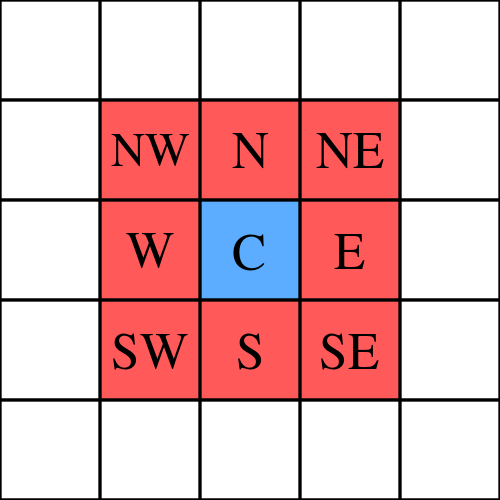
\includegraphics[width=0.5\textwidth]{../img/w12-lab/moore_neighborhood.png}
  \end{center}
  \caption{Moore-grannskapet består av nio celler: mittcellen samt de åtta omringande cellerna.\protect\footnotemark}
  \label{fig:threads:life:moore-neighborhood}
\end{figure}
\footnotetext{Källa: \url{https://commons.wikimedia.org/wiki/File:Moore_neighborhood_with_cardinal_directions.svg}}


\subsection{Beskrivning av Workspace}

I workspacet finner ni bl.a. paketen \code{models}, \code{rules} och \code{views}. I labben kommer ni främst ändra i \code{models}-paketet, men ni kommer även implementera reglerna för Life i \code{rules/LifeRule.scala}. Paketet \code{views} kommer med färdigimplementerad kod för två vyer \code{CellularConsoleView} samt \code{CellularGuiView}.

Utöver paketen finner ni i samma mapp några körbara Scala-filer som kan användas för att starta upp ett användargränssnitt som ritar upp brädet och låter användaren `spela' spelet. Den första av dessa filerna ni ska titta i och senare köra är \code{life.scala}.

Läs igenom de två filerna i \code{models}-paketet noga. Det är där ni kommer spendera den mesta av tiden.


\subsection{Obligatoriska uppgifter}
	% Förslag på hur de kan bygga upp programmet:
    % 1) skapa en main-klass som öppnar ett fönster som visar ett x gånger y stort fönster.
    % 2) [Kommer inte göras] skapa en klass Cell som har attributet levande eller död. Gör en metod där man kan ändra tillståndet på cellen.
    % 3) skapa en matris av celler som alla initieras som döda.
	% 4) koppla ihop modellen och vyn så att om man genom att klicka i vyn kan ändra cellens tillstånd. Testa att det fungerar. Gör så att vyn uppdateras efter cellerna i modellen när man klickar på "next generation".
	% 5) Studera traitet Rule i filen blahblah. Implementera reglerna (ge lite förklarande kodexempel för traitet Rule eller var det finns)
	% 6) Skriv metod(er) som räknar upp generationer.
	% 7) Testa nedanstående startfigurer (inkludera bilder på t ex en slider). Beter det sig som förväntat?


\Task Skapa en modell som kan visas i vyer som implementerar \code{CellularView2D}.

Spelbrädet består av en matris med $n$ rader och $m$ kolumner. ($n$ och $m$ brukar ibland modelleras som $\infty$, men vi kommer begränsa oss för enkelhetens skull).

Varje cell i matrisen kan vid varje tidpunkt (i varje generation) ha ett av två tillstånd: levande eller död. Dessa kommer vi för enkelhetens skull att representera som 1 eller 0, respektive. Detta för att göra det enklare att räkna ihop hur många levande grannar en cell har.

\Subtask Implementera konstruktorn i kompanjonsobjektet för \code{ArrayMatrix2D}.

För att skapa en matris ska vi använda oss av Scalas inbyggda datastruktur \code{Array}. Denna datastruktur har en användbar konstruktur \code{ofDim[T](n1: Int, n2: Int)} som vi ska använda för att skapa \emph{rows} stycken arrayer av storlek \emph{cols} inuti en annan array.

Ett exempel av resultatet från \code{Array.ofDim[Int](3, 3)} är följande ekvivalenta kod:

\begin{Code}
Array(
	Array(0,0,0),
	Array(0,0,0),
	Array(0,0,0)
)
\end{Code}

% Här nedan ser vi en sådan array utskriven i en komma-separerad lista. Detta är ett vanligt och enkelt dataformat som kallas CSV.\footnote{Förkortningen CSV står för Comma Separated Values}

%\begin{Code}
%0,0,0
%0,0,0
%0,0,0
%\end{Code}

\Subtask Implementera de övriga metoderna i \code{ArrayMatrix2D}. Läs igenom kommentarerna för de oimplementerade metoderna i traitet \code{Matrix2D} för kommentarer om vad som ska göras.


\Subtask Testa implementationen. Ta gärna hjälp av metoden \code{randomize} som finns på alla objekt som ärver traitet \code{Matrix2D}. Med den kan man enkelt slumpa fram nya tillstånd på brädet på följande vis:

\begin{Code}
// Slumpar varje cell i matrisen 'matrix' till antingen 0 eller 1
matrix.randomize(2)
\end{Code}

För att nu kontrollera att allt har blivit rätt kan vi visa upp matrisen i terminalen med hjälp av \code{CellularConsoleView}. Ett exempel på detta finns i \code{life_console.scala}.

\begin{Code}
// Skriver ut brädet i konsolen
CellularConsoleView.display(matrix)
\end{Code}

Men detta testar inte för alla möjliga fel, så för säkerhets skull kan vi även testa att placera ut en s.k. glider i brädet med hjälp av metoden \code{place} som finns implementerad i det ärvda traitet \code{Matrix2D}.

\begin{Code}
// Placerar ut en glider med sitt övre vänstra hörn i punkten
// (3, 1), d.v.s. på rad 4 och kolumn 2 (då vi noll-indexerar)
matrix.place(entities.glider, 3, 1)
\end{Code}

\begin{figure}[h]
  \begin{center}
    % Reflectbox here since glider in entities package is a reflection of the image.
    \reflectbox{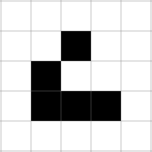
\includegraphics[width=0.3\textwidth]{../img/w12-lab/glider.png}}
  \end{center}
  \caption{En så kallad \textit{glider}. Vanligt förekommande varelse i Life.}
  \label{fig:threads:life:glider}
\end{figure}

Testa nu att rita ut brädet igen (utan \code{randomize} den här gången) för att se till att glidern hamnade rätt både med avseende på orientering och position. Den ska vara roterad precis som i figur \ref{fig:threads:life:glider}.


\Task Implementera Life-regeln med hjälp av traitet \code{Rule}.

Nu har vi vår datastruktur för brädet på plats, så det är dags att faktiskt implementera reglerna för Life. För att göra detta ska vi implementera objektet \code{LifeRule} som ärver traitet \code{Rule} vilket är ett interface som cellulära automaters regler kan implementera. Men först ska vi implementera några hjälpsamma funktioner, så att vår kod i \code{LifeRule} senare blir mer lättläst.

\Subtask Implementera \code{mooreNeighborsPositions} samt \code{mooreNeighborsStates} i \code{Matrix2D}.

Då Life-regeln förlitar sig på Moore-grannskapet som tidigare nämnts så behöver vi ett smidigt sätt att få ut grannarna för en viss cell. Detta är vad funktionerna \code{mooreNeighborsPositions} samt \code{mooreNeighborsStates} ska göra.

När \code{mooreNeighborsStates} implementeras är det viktigt att ta hänsyn till om grannarna faktiskt finns (då vårt bräde är av begränsad storlek).
För detta bör man använda \code{isWithinMatrix}-metoden som tidigare implementerades i \code{ArrayMatrix2D}.

Börja med att implementera \code{mooreNeighborsPositions} och använd sedan den för att implementera \code{mooreNeighborsStates}.

\Subtask Implementera \code{apply} i ett nytt objekt \code{LifeRule} som implementerar \code{Rule}.

Nedan finns specifikationen för traitet \code{Rule}. Den innehåller endast en metod \code{apply} vars uppgift är att ta ett bräde samt en position på brädet och returnera vad denna position ska innehålla för värde i nästa generation.

\begin{ScalaSpec}{Rule}
// apply tar en matris samt en position i matrisen (row, col)
// och applicerar regeln på den positionen
def apply(m: ArrayMatrix2D, row: Int, col: Int): Int
\end{ScalaSpec}

Reglerna för Life finner ni ovan i avsnitt \ref{subsec:life-rules}.

\Subtask Testa implementationen.

För att nu i praktiken applicera vår regel på brädet ska vi använda oss av metoden \code{applyRule} som finns i \code{ArrayMatrix2D}.

Om man har problem med att sin regel inte beter sig som förväntat kan man felsöka genom att returnera antalet grannar istället för cellens levande/död-tillstånd. Efter att ha applicerat hela s.k. \code{NeighborsRule} kan man visa upp resultatet med \code{CellularConsoleView} för att se om programmet räknar grannar korrekt.


\Task Skapa en ny modell som ''wrappar'' i kanterna.

Just nu har vi ett udda beteende i modellen, nämligen att alla celler utanför brädet i praktiken räknas som döda. För att få ett lite mer intressant beteende vill vi nu göra så att om exempelvis en glider åker in i höger vägg ska den komma ut ur vänster vägg. Detta kan göras med några små modifikationer till \code{ArrayMatrix2D}.

\Subtask Ändra metoden \code{isWithinMatrix} så att alla positioner är giltiga.

Då funktionen \code{mooreNeighborsStates} i \code{Matrix2D} använder sig av funktionen \code{isWithinMatrix} för att avgöra om celler är inom brädet måste vi se till att \code{isWithinMatrix} inte hindrar grann-funktionen från att hämta celler ''utanför'' brädet. Detta kan vi enkelt göra genom att kommentera ut hela den tidigare koden och istället alltid returnera \code{true}. Om vi nu försöker köra programmet kommer vi få \code{ArrayIndexOutOfBoundsException} eftersom vi ännu inte gjort så att hämtningar eller tilldelningar ''utanför'' brädet wrappar, vilket vi nu ska göra.

\Subtask Ändra metoderna \code{get} samt \code{set} så att hämtningar respektive tilldelningar utanför brädet wrappar.

För att åstadkomma wrappning måste vi göra så att alla hämtningar och tilldelningar utanför brädet ''går runt''. Detta kan enklast göras med hjälp av modulo-operatorn.

\begin{Code}
val wrapped_row = row % rows
\end{Code}

Men denna lösning tar inte hänsyn till negativa tal, vilket kan uppkomma när man t.ex. försöker hämta grannarna för cellen i det övre vänstra hörnet på brädet, d.v.s. position (0, 0). För att enkelt lösa detta kan man förskjuta hela \code{row} med \code{rows} så att man istället får följande:

\begin{Code}
val wrapped_row = (rows + row) % rows
\end{Code}

Vi kan använda oss av denna kunskap för att i metoderna \code{get} samt \code{set} se till att operationerna wrappar. Testa sedan din implementation genom att låta en glider glida in i en vägg.


\subsection{Frivilliga extrauppgifter}

Inom cellulära automata finns det många intressanta ting att utforska. Nedan finns några extrauppgifter som nyfikna och intresserade läsare uppmanas implementera då resultaten kan vara djupt tillfredställande. De kan göras i valfri ordning.


\Task Implementera spara och ladda.

När man leker runt med cellulära automater vill man ofta spara sina bräden så att man senare enkelt kan ladda in dem igen. För att göra detta ska vi i denna extrauppgift definiera ett dataformat som ska innehålla all data som behövs för att återskapa vår \code{ArrayMatrix2D}.

\Subtask Spara brädets tillstånd.

Tillståndet ska sparas till ett format som både är lätt att spara/exportera och ladda/importera. Det vi behöver spara är följande:

\begin{itemize}
	\item Brädets storlek, d.v.s. antalet rader och kolumner
	\item Hur många olika värden en cell på brädet kan anta
	\item Matrisen i sig, d.v.s. alla cellers värden
\end{itemize}

Det är metoden \code{ArrayMatrix2D.toFileFormat} som ska implementeras.

Vi föreslår att ni börjar filen med en rad innehållande de två värdena i punkt ett, samt värdet i punkt två. Separera dem med mellanslag, komma, eller en emoji (på egen risk). Därefter är det lämpligt att skriva ut matrisen rad för rad där varje cell skrivs ut som en etta eller nolla. Man kan göra detta utan separator för bräden där celler bara antar värden i intervallet 0-9, men det fungerar inte längre om en cell kan anta andra värden (såsom i uppgiften med cykliska cellulära automater nedan) då man inte längre kan lita på att en cell motsvaras av en enda siffra. För att lösa denna begränsning kan man separera sina värden med något tecken precis som för första raden.

Testa att spara genom att gå in i menyn i användargränssnittet och välja ''Save...''. Öppna den sparade filen med en texteditor för att verifiera att innehållet ser korrekt ut.

\Subtask Ladda in det sparade tillståndet.

Implementera metoden \code{ArrayMatrix2D.fromFileFormat} för att läsa in det sparade tillståndet.

Testa sedan att ladda genom att gå in i menyn i användargränssnittet och välja ''Load...''. Brädet ska nu se ut precis som det gjorde när det sparades.

\Task Implementera andra regler för cellulära automata.

Det finns massor med regler för cellulära automata med sina egna intressanta beteenden och tillstånd.
Gör den eller de du tycker verkar mest intressant!

Fler regler finns här: \url{https://en.wikipedia.org/wiki/Category:Cellular_automaton_rules}

Nedan följer några roliga exempel som valts ut och anses lämpliga.

\Subtask Implementera regeln för cykliska cellulära automater.

Denna typ av automata kallas cyklisk just för att det finns $N$ möjliga tillstånd och när tillståndet $N-1$ nås så är ''nästa'' tillstånd $0$.
Detta beteende kan beskrivas med modulo-operatorn: $T_{nästa} = (T_{nuvarande} + 1)\ \%\ N$

Regeln är att om en granne till den aktuella cellen har tillståndet exakt ett över cellens tillstånd så får cellen sin grannes tillstånd. Det vill säga om en granne har tillståndet $T_{nästa}$ så får även cellen i mitten det värdet.

För att få intressant beteende brukar man initialisera hela brädet så att varje cell får ett slumpvalt tillstånd.

En bra förberedelse för att implementera denna cellulära automat är att läsa Wikipedia-artikeln: \url{https://en.wikipedia.org/wiki/Cyclic_cellular_automaton}

    \Subtask{Implementera regeln för Wireworld.}

Wireworld skiljer sig från andra cellulära automata då man i Wireworld designar `kretsar' inte helt olika de som finns i moderna datorer.
På grund av detta är majoriteten av celler vanligtvis fast i ett dött tillstånd (isolatorer).

I Wireworld kan man skapa komponenter såsom dioder och transistorer. Med dessa kan man bygga logiska grindar och därmed hela datorer (som dock blir väldigt långsamma i jämförelse med datorerna de körs på).

En bra förberedelse för att implementera Wireworld är att läsa Wikipedia-artikeln: \url{https://en.wikipedia.org/wiki/Wireworld}

\begin{figure}[h]
    \begin{center}
        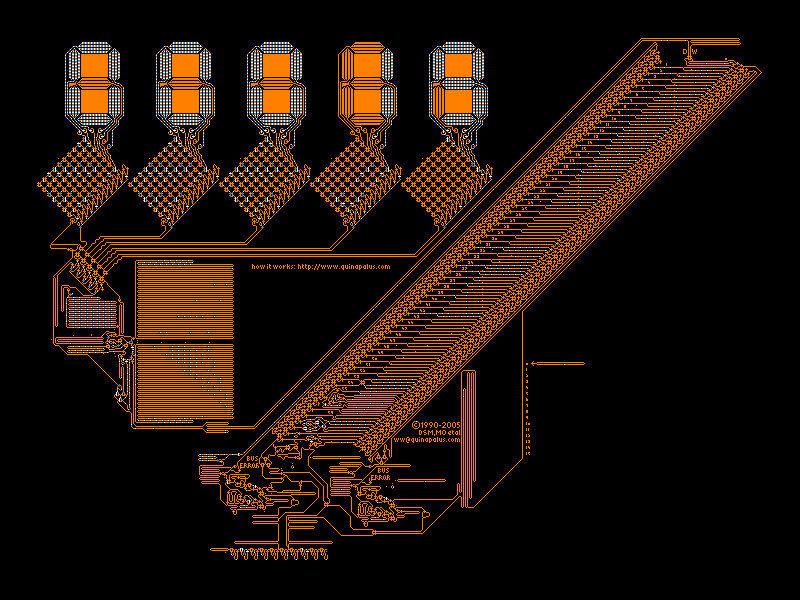
\includegraphics[width=0.8\textwidth]{../img/w12-lab/wireworld_computer.png}
    \end{center}
    \caption{En enkel dator implementerad i Wireworld.\protect\footnotemark}
    \label{fig:threads:life:wireworld-computer}
\end{figure}
\footnotetext{Källa: \url{http://www.quinapalus.com/wi-index.html}}


\subsection{Extra läsning}

\begin{itemize}

\item[] \textbf{Intressanta mönster i Life}

\begin{itemize}[noitemsep,topsep=0pt]
    \item \url{https://en.wikipedia.org/wiki/Spacefiller}
    \item \url{https://en.wikipedia.org/wiki/Spaceship_(cellular_automaton)}
\end{itemize}

\item[] \textbf{Intressanta automater}

\begin{itemize}[noitemsep,topsep=0pt]
	\item \url{https://en.wikipedia.org/wiki/Codd's_cellular_automaton}
	\item \url{https://en.wikipedia.org/wiki/Von_Neumann_universal_constructor}
\end{itemize}

\item[] \textbf{Intressanta resurser}

\begin{itemize}[noitemsep,topsep=0pt]
    \item Eric Weisstein's Treasure Trove of the Life Cellular Automaton: \\ \url{http://www.ericweisstein.com/encyclopedias/life/topics/}
\end{itemize}

\end{itemize}


% Kanske för nästa år
%\Task{Alternativ vy: Kör programmet i webbläsaren med Scala.js}


% Detta kan kräva speciell IDE (android-studio) och eventuellt en Android-emulator som inte kan köras på skolans datorer.
%\Task{Alternativ vy: Kör programmet på Android}


% Detta kommer antagligen inte ske då det lägger till signifikant komplexitet
% En bättre extrauppgift är att representera brädet som ett quadtree då det leder en in på Hashlife
%\Task{Implementera brädet som en sparse-matris}

%I den tidigare lösningen har vi allokerat en hel matris där bara en del av brädet vanligtvis är levande, en sådan matris kallas för en sparse matris (en matris där majoriteten av värdena är 0).
%    \Subtask{???}


%\Task{Implementera den supersnabba Hashlife}
%    Detta är en utmaning som kräver en viss kunskap om algoritmer och hashning som läsare av denna labben inte ännu förväntas inneha.
%    Den verkligt intresserade läsaren kan dock se denna uppgift som ett långtids-läromål och återkomma till uppgiften senare i sin utbildning när
%    hen känner sig redo.
%
%    En utförlig beskrivning om hashlife och quadtrees finnes på Wikipedia:
%    \begin{enumerate}
%        \item https://en.wikipedia.org/wiki/Hashlife
%        \item https://en.wikipedia.org/wiki/Quadtree
%    \end{enumerate}
%
%    \Subtask{Implementera QuadtreeMatrix2D}
%        Hashlife använder sig inte av en matris-representation för brädet utan använder sig istället av en datastruktur som heter Quadtrees.
%        Dessa fungerar som vanliga träd fast varje nod kan antingen ha exakt 4 brancher eller vara ett löv. Varje branchning delar upp en kvadrat
%        i 4 mindre kvadrater och varje löv representerar värdet för en kvadrat.
%
%        Quadtrees möjliggör att man kan beräkna tomma områden på brädet på konstant tid då man vet att ett helt område kommer förbli opåverkat utan
%        att behöva titta igenom varje cell.
%
%        \begin{figure}[h]
%            \begin{center}
%                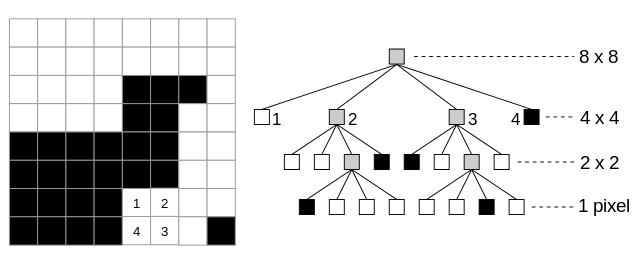
\includegraphics[width=0.7\textwidth]{../img/w12-lab/quadtree_bitmap.png}
%            \end{center}
%            \caption{Ett exempel på hur ett Quadtree använts för att representera en bitmap likt den som återfinns i Life}
%            % Källa: Wikipedia (https://commons.wikimedia.org/wiki/File:Quad_tree_bitmap.svg)
%        \end{figure}
%
%    \Subtask{Implementera hashlife}
%
%        Här kan vi inte handleda er, då det anses vara allt för långt utanför kursmålen. Men för den ambitiösa studenten refererar vi glatt till Wikipedia och önskar er lycka till!

%!TEX encoding = UTF-8 Unicode
%!TEX root = ../compendium2.tex

\Assignment{bank}

\subsection{Fokus}
\begin{itemize}[nosep,label={$\square$},leftmargin=*]
\item Kunna implementera ett helt program efter given specifikation
\item Kunna sätta samman olika delar från olika moduler
\item Förstå hur Java-klasser kan användas i Scala
\item Förstå och bedöma när immutable/mutable såväl som var/val bör användas i större sammanhang
\item Kunna använda sig av kompanjonsobjekt
\item Kunna läsa och skriva till fil
\item Kunna söka i olika datastrukturer på olika sätt
\end{itemize}

\subsection{Bakgrund}

I detta projekt ska du skriva ett program som håller reda på bankkonton och kunder i en bank. Programmet ska utöver att hålla reda på bankens nuvarande tillstånd även föra historik över alla tillståndsändringar. Historiken ska vara så pass detaljerad att det nuvarande tillståndet kan återskapas genom att återuppspela alla ändringar som finns lagrade i historiken.

Programmet ska vara helt textbaserat, man ska alltså interagera med programmet via terminalen där en meny skrivs ut och input görs via tangentbordet.

Du ska skriva större delen av programmet själv, utan någon färdig kod. Programmet ska dock följa de specifikationer som ges i uppgiften, såväl som de objektorienterade principer du lärt dig i kursen.

\subsection{Krav}

Kraven för bankapplikationen återfinns här nedan. För att bli godkänd på denna uppgift måste samtliga krav uppfyllas:

\begin{itemize}
\item Programmet ska ha följande menyval:

\begin{itemize}
\item 1. Hitta konton för en viss kontoinnehavare med angivet ID.
\item 2. Söka efter kunder på (del av) namn.
\item 3. Sätta in pengar på ett konto.
\item 4. Ta ut pengar på ett konto.
\item 5. Överföra pengar mellan två olika konton.
\item 6. Skapa ett nytt konto.
\item 7. Ta bort ett befintligt konto.
\item 8. Skriv ut bankens alla konton, sorterade i bokstavsordning efter innehavare.
\item 9. Återställa banken till tillståndet den hade vid ett givet datum. För enkelhetens skull får du permanent kassera all historik som skapades efter det datum banken återställs till.
\item 10. Avsluta.
\end{itemize}

\item När något av följande sker ska programmet notera det i historiken:
\begin{itemize}
\item Pengar sätts in på ett konto.
\item Pengar tas ut från ett konto.
\item Pengar överförs mellan två konton.
\item Ett konto skapas.
\item Ett konto tas bort.
\end{itemize}
\item Historiken ska sparas både i minnet och i en fil.
\item Då programmet startas ska det läsa in historikfilen för att återskapa tillståndet som banken hade tidigare.
\item Allt som berör användargränssnittet (såsom utskrifter till terminalen och inläsning från terminalen) ska ske i \code{BankApplication} eller hjälpklasser till \code{BankApplication}, inte i någon annan av klasserna som specificeras i uppgiften.
\item Alla metoder och attribut ska ha lämpliga åtkomsträttigheter.
\item Valen av val/var och immutable/mutable måste vara lämpliga.
\item Din indata måste ge samma resultat som i exemplen i bilagan.
\item Rimlig felhantering ska finnas. Det är alltså önskvärt att programmet inte kraschar då man matar in felaktig input, utan istället säger till användaren att input är ogiltlig.
\item Programdesignen ska följa de specifikationer som är angivna nedan.
\item Det räcker med att banken ska kunna hantera heltal, men detta ska göras med klassen \code{BigInt}.
\item Klassen \code{BankAccount} ska generera ett unikt kontonummer för varje konto. Dessa ska återställas om bankens tillstånd återställs till ett tidigare datum, d.v.s. att om en återställning av banken tar bort ett konto så ska dess kontonummer återigen bli tillgängligt.
\end{itemize}

\subsection{Design}
Nedan följer specifikationerna för de olika klasserna bankapplikationen måste innehålla:

\begin{ScalaSpec}{Customer}
/**
 * Describes a customer of a bank with provided name and id.
 */
case class Customer(name: String, id: Long) = {
	override def toString(): String = ???
}
\end{ScalaSpec}


\begin{ScalaSpec}{BankAccount}
/**
 * Creates a new bank account for the customer provided.
 * The account is given a unique account number and initially
 * has a balance of 0 kr.
 */
class BankAccount(val holder: Customer) = {

  /**
   * Deposits the provided amount in this account.
   */
  def deposit(amount: Int): Unit = ???

  /**
   * Returns the balance of this account.
   */
  def getBalance: Int = ???

  /**
   * Withdraws the provided amount from this account,
   * if there is enough money in the account. Returns true
   * if the transaction was successful, otherwise false.
   */
  def withdraw(amount: Int): Boolean = ???
}
\end{ScalaSpec}


\begin{ScalaSpec}{Bank}
/**
 * Creates a new bank with no accounts and no history.
 */
class Bank() = {

 /**
   * Returns a list of every bank account in the bank.
   * The returned list is sorted in alphabetical order based
   * on customer name.
   */
  def getAllAccounts(): Vector[BankAccount] = ???

  /**
   * Returns the account holding the provided account number.
   */
  def findByNumber(accountNbr: Int): Optional[BankAccount] = ???

  /**
   * Returns a list of every account belonging to
   * the customer with the provided id.
   */
  def findAccountsForHolder(id: Long): Vector[BankAccount] = ???

  /**
   * Returns a list of all customers whose names match
   * the provided name pattern.
   */
  def findByName(namePattern: String): Vector[Customer] = ???

 /**
   * Executes an event in the bank.
   * Returns a string describing whether the
   * event was successful or failed.
   */
  def doEvent(event: BankEvent): String = ???

  /**
   * Resets the bank to the state it had at the provided date.
   * Returns a string describing whether the event was
   * successful or failed.
   */
  def returnToState(returnDate: Date): String = ???
}
\end{ScalaSpec}


Till din hjälp innehåller kursens workspace följande färdigskrivna klasser:
\begin{itemize}
\item \code{Date}, en enkel wrapper av \code{Java.time} som du ska använda för att representera tidsstämplar.
\item \code{BankEvent} med tillhörande subtyper, som du ska använda för att representera förändringar av bankens tillstånd.
\end{itemize}


\subsection{Tips}

\begin{itemize}
\item Det enda sättet att förändra tillståndet för en \code{Bank} ska vara (förutom att anropa \code{returnToState}) att anropa \code{doEvent} med en \code{BankEvent} som beskriver tillståndsförändringen. Vid en första anblick kan detta kan verka lite väl bökigt, men när ändringshistoriken ska implementeras kommer det vara till stor hjälp att det finns en \code{BankEvent} som representerar varje ändring.

\item För att skriva till fil på ett enkelt sätt kan man t.ex. använda sig av statiska metoder i klassen \code{Files} som finns tillgänglig i \code{java.nio.file}. För att undvika portabilitetsproblem kan man då använda sig av ett bestämt \code{Charset}, t.ex. \code{UTF_8}, som finns tillgänglig i \code{java.nio.charset.StandardCharsets.UTF_8}.

\item För att läsa ifrån en fil kan man t.ex. använda sig av \code{Source} som finns tillgänglig i \code{scala.io.Source}.

\item Var noggrann med att testerna klarar alla tänkbara fall, och tänk på att fler fall än dem som givits i exempel kan förekomma vid rättning.
\end{itemize}

\subsection{Obligatoriska uppgifter}

\Task Implementera klassen \code{Customer}.

\Task Implementera klassen \code{BankAccount}.

\Task Skapa singelobjektet \code{BankApplication}, som ska innehålla \code{main}-metoden. Det kan vara bra att innan man fortsätter se till att denna skriver ut menyn korrekt och kan ta input från tangentbordet som motsvarar de menyval som finns.

\Task Implementera klassen \code{Bank}.

\Subtask Implementera menyval 6 och 8. Testa noga.

\Subtask Implementera ändringshistoriken. Varje gång \code{doEvent} anropas ska dess \code{BankEvent}-argument läggas till i historiken tillsammans med det nuvarande datumet.

\Subtask Implementera alla andra menyval, förutom menyval 9. Testa de nya menyvalen noga efterhand som du implementerar dem, i synnerhet så att ändringshistoriken fungerar korrekt. Gör de utökningar du anser behövs.

\Task Implementera säkerhetskopiering av historiken.

\Subtask När en \code{BankEvent} läggs till i historiken ska den också skrivas till en historikfil omedelbart. Banken ska ej behöva avslutas för att utskriften ska hamna på fil, om så vore fallet kan information gå förlorad om banken kraschar.

I workspace-katalogen för denna projektuppgift finns en historikfil bifogad. För bekvämlighet finns ett utdrag av denna fil infogad nedanför. Inläsning och utskrift ska ske med dess format:\\~\\
2016 3 7 10 6 N 850127 Fredrik\newline
2016 3 7 10 28 D 1000 16500\newline
2016 3 9 10 52 W 1000 3900\newline
2016 3 9 11 8 N 900318 Casper\newline
2016 3 9 16 28 D 1001 6500\newline
2016 4 1 10 11 W 1001 1900\newline
2016 4 1 11 19 W 1001 2000\newline
2016 4 2 16 33 N 651002 Björn\newline
2016 4 2 16 46 D 1002 25000\newline
2016 4 3 10 11 T 1002 1000 4000\\~\\
Formen är alltså:\\~\\
\textbf{År  Månad  Dag  Timme  Minut  BankEventTag  Parametrar}
\\~\\
De olika klasserna av \code{BankEvent} representeras med följande bokstav:

\begin{itemize}
\item D - \code{Deposit}
\item W - \code{Withdraw}
\item T - \code{Transfer}
\item N - \code{NewAccount}
\item E - \code{DeleteAccount}
\end{itemize}

\Subtask När programmet startar ska det läsa in alla händelser från historikfilen och återuppspela dem en efter en. På så sätt kan bankens tillstånd återställas, fastän vi bara har sparat ändringshistoriken och inte själva tillståndet.

\Task Implementera menyval 9 genom att först nollställa bankens tillstånd och sedan återuppspela allt i historiken som hände före det givna datumet. Resten av historiken bör tas bort permanent, både i minnet och i historikfilen.


\subsection{Frivilliga extrauppgifter}

Gör först klart projektets obligatoriska delar. Därefter kan du, om du vill, utöka ditt program enligt följande.

\Task Skriv en eller flera av klasserna \code{Customer} och \code{BankAccount} i Java istället och använd dig av dessa i din Scala-kod.

\Task	Implementera ett nytt menyalternativ som skriver ut all kontohistorik för en given person. I historiken ska finnas typ av händelse med tillhörande parametrar, dåvarande saldo vid händelsen, såväl som datumet för händelsen.

\subsection{Exempel på körning av programmet}

Nedan visas möjliga exempel på körning av programmet. Data som matas in av användaren är markerad i fetstil.
Ditt program måste inte se identiskt ut, men den övergripande strukturen såväl som resultat av körningen ska vara densamma.
När det första exemplet börjar förutsätts det att banken inte har några konton.

Listan över val, som är markerad i kursiv stil i det första exemplet, är inte utskriven i senare exempel för att spara plats på pappret. Ditt program ska alltid skriva ut listan över val före användaren ska mata in ett val.

% This environment uses minipage to prevent column breaks from occurring in the middle of an example
\newenvironment{exampleblock}
	{\begin{minipage}{\columnwidth}
	 - - - - - - - - - - - - - - - - - - - - - - - - - - -\\}
	{\end{minipage}}

\begin{multicols}{2}
\noindent
\begin{exampleblock}
\textit{
1.   Hitta ett konto för en given kund\\
2.   Sök efter kunder på (del av) namn\\
3.   Sätt in pengar\\
4.   Ta ut pengar\\
5.   Överför pengar mellan konton\\
6.   Skapa nytt konto\\
7.   Radera existerande konto\\
8.   Skriv ut alla konton i banken\\
9.   Återställ banken till ett tidigare datum\\
10.  Avsluta\\
}
Val: \textbf{6}\\
Namn: \textbf{Adam Asson}\\
Id: \textbf{6707071234}\\
Nytt konto skapat med kontonummer: 1000\\
10:03:0 CET 14 / 5 - 2016\\
\end{exampleblock}
\begin{exampleblock}
Val: \textbf{1}\\
Id: \textbf{6707071234}\\
Konto 1000 (Adam Asson, id 6707071234) 0 kr\\
10:04:0 CET 14 / 5 - 2016\\
\end{exampleblock}
\begin{exampleblock}
Val: \textbf{6}\\
Namn: \textbf{Berit Besson}\\
Id: \textbf{8505255678}\\
Nytt konto skapat med kontonummer: 1001\\
10:12:0 CET 14 / 5 - 2016\\
\end{exampleblock}
\begin{exampleblock}
Val: \textbf{2}\\
Namn: \textbf{adam}\\
Adam Asson, id 6707071234\\
10:15:0 CET 14 / 5 - 2016\\
\end{exampleblock}
\begin{exampleblock}
Val: \textbf{8}\\
Konto 1000 (Adam Asson, id 6707071234) 0 kr\\
Konto 1001 (Berit Besson, id 8505255678) 0 kr\\
10:13:0 CET 14 / 5 - 2016\\
\end{exampleblock}
\begin{exampleblock}
Val: \textbf{6}\\
Namn: \textbf{Berit Besson}\\
Id: \textbf{8505255678}\\
Nytt konto skapat med kontonummer: 1002\\
13:56:0 CET 14 / 5 - 2016\\
\end{exampleblock}
\begin{exampleblock}
Val: \textbf{2}\\
Namn: \textbf{erit}\\
Berit Besson, id 8505255678\\
14:01:0 CET 14 / 5 - 2016\\
\end{exampleblock}
\begin{exampleblock}
Val: \textbf{3}\\
Kontonummer: \textbf{1000}\\
Summa: \textbf{5000}\\
Transaktionen lyckades.\\
14:36:0 CET 14 / 5 - 2016\\
\end{exampleblock}
\begin{exampleblock}
Val: \textbf{5}\\
Kontonummer att överföra ifrån: \textbf{1000}\\
Kontonummer att överföra till: \textbf{1001}\\
Summa: \textbf{1000}\\
Transaktionen lyckades.\\
14:37:0 CET 14 / 5 - 2016\\
\end{exampleblock}
\begin{exampleblock}
Val: \textbf{8}\\
Konto 1000 (Adam Asson, id 6707071234) 4000 kr\\
Konto 1001 (Berit Besson, id 8505255678) 1000 kr\\
Konto 1002 (Berit Besson, id 8505255678) 0 kr\\
14:52:0 CET 14 / 5 - 2016\\
\end{exampleblock}
\begin{exampleblock}
Val: \textbf{7}\\
Ange konto att radera: \textbf{1002}\\
Transaktionen lyckades.\\
14:01:0 CET 14 / 5 - 2016\\
\end{exampleblock}
\begin{exampleblock}
Val: \textbf{8}\\
Konto 1000 (Adam Asson, id 6707071234) 4000 kr\\
Konto 1001 (Berit Besson, id 8505255678) 1000 kr\\
14:01:0 CET 14 / 5 - 2016\\
\end{exampleblock}
\begin{exampleblock}
Val: \textbf{9}\\
Vilket datum vill du återställa banken till?\\
År: \textbf{2016}\\
Månad: \textbf{5}\\
Datum (dag): \textbf{9}\\
Timme: \textbf{18}\\
Minut: \textbf{10}\\
Banken återställd.\\
15:00:0 CET 14 / 5 - 2016\\
\end{exampleblock}
\begin{exampleblock}
Val: \textbf{8}\\
Konto 1002 (Björn, id 651002) 25900 kr\\
Konto 1001 (Casper, id 900318) 4600 kr\\
Konto 1003 (Eva, id 950908) 6300 kr\\
Konto 1000 (Fredrik, id 850127) 11800 kr\\
Konto 1004 (Kajsa, id 810722) 17000 kr\\
15:01:0 CET 14 / 5 - 2016\\
\end{exampleblock}
\begin{exampleblock}
Val: \textbf{3}\\
Kontonummer: \textbf{1005}\\
Summa: \textbf{5000}\\
Transaktionen misslyckades. Inget sådant konto hittades.\\
15:06:0 CET 14 / 5 - 2016\\
\end{exampleblock}

\end{multicols}

%!TEX encoding = UTF-8 Unicode
%!TEX root = ../compendium.tex

\Assignment{tictactoe}

\subsection{Obligatoriska uppgifter}

\Task En uppgift.

\Subtask En underuppgift.

\Subtask En underuppgift.

\subsection{Frivilliga extrauppgifter}

\Task En uppgift.

\Subtask En underuppgift.

\Subtask En underuppgift.
%!TEX encoding = UTF-8 Unicode
%!TEX root = ../compendium.tex

\Assignment{imageprocessing}

\subsection{Bakgrund}

En digital bild består av ett rutnät (en matris) av pixlar. Varje pixel har en färg, och om man har många pixlar flyter de samman för ögat så att de tillsammans skapar en bild.

Det finns olika system för hur man färgsätter de olika pixlarna. T.ex. så används CMYK-systemet (cyan, magenta, gul, svart) vid blandning av färg som ska tryckas på papper eller annat material. På en dator däremot används vanligtvis RGB-systemet. RGB-systemet har tre grundfärger: röd, grön och blå. Mättnaden av varje grundfärg anges av ett heltal som vi i fortsättningen förutsätter ligger i intervallet [0, 255]. 0 anger ”ingen färg” och 255 anger ”maximal färg”. Man kan därmed representera 256 × 256 × 256 = 16 777 216 olika färgnyanser. Man kan också representera gråskalor; det gör man med färger som har samma värde på alla tre grundfärgerna: (0, 0, 0) är helt svart, (255, 255, 255) är helt vitt.


\subsection{Uppgiften}
Du ska skriva ett program där du implementerar olika filter som ska manipulera en given bild på ett flertal olika sätt. Filterklasserna ska ärva från en abstrakt \code{ImageFilter}-klass som är skriven i Java. \code{ImageFilter}-klassen hittar du i cslib.

Följande beskriver \code{ImageFilter}-klassen.

\begin{JavaSpec}{abstract class ImageFilter}
/**
 * Skapar ett filterobjekt med ett givet namn.
 */
protected ImageFilter(String name);

/**
 * Tar reda på filtrets namn.
 */
public String getName();

/**
 * Filtrerar bilden i matrisen inPixels och returnerar
 * resultatet i en ny matris. Utnyttjar eventuellt 
 * värdet av paramValue
 */
public abstract Color[][] apply(Color[][] inPixels,
				 double paramValue);

/**
 * Berättar huruvida ett filter behöver ett parmetervärde eller inte
 * @return true ifall parametervärde behövs, annars false
 */
public abstract boolean needsParameter();

/**
 * Beräknar intensiteten hos alla pixlarna i pixels,
 * returnerar resultatet i en ny matris.
 */
protected short[][] computeIntensity(Color[][] pixels):

/**
 * Faltar punkten p[i][j] med faltningskärnan kernel.
 * 
 * @param p 		matris med talvärden
 * @param i 		radindex får den aktuella punkten
 * @param j 		kolonnindex får den aktuella punkten
 * @param kernel	faltningskärnan, en 3x3-matris
 * @param weight	summan av elementen i kernel
 * @return 		resultatet av faltningen
 */
protected short convolve(short[][] p, int i, int j, 
			short[][] kernel, int weight);
\end{JavaSpec}

Utöver filterklasserna ska du även skapa ett program där du kan välja ett variabelt antal filter och sedan applicera dessa på en bild. För att åstadkomma detta ska du implementera klasserna \code{FilterChooser}, som hanterar val av filter, och \code{FilterList} som representerar vilka filter som ska användas. Klasserna har följande specifikationer:

\begin{ScalaSpec}{FilterList}
class FilterList = ???

/** Adds a filter to the FilterList */
def addFilter(filter: ImageFilter): Unit = ???
  
/** Applies all the filters on the given Image and draws it in SimpleWindow */
def applyFilters(image: Image, sw: SimpleWindow): Unit = ???
\end{ScalaSpec}

\begin{ScalaSpec}{FilterChooser}
/** Creates a FilterChooser with all the available filters */
class FilterChooser(filters: Array[ImageFilter]) = ???
  
/** Shows which filters are available and lets the user choose filters
*   until an escape sequence has been given and returns a FilterList which
*   contain the chosen filters
*   Example: 
*   Tryck på 1 för Blått-filter
*   Tryck på 2 för Kontrast-filter
*   Tryck på 3 för Gauss-filter
*   Tryck på 4 för Sobel-filter
*   Tryck 42 om du inte vill ha fler filter
*/
def chooseFilters(): FilterList = ???
\end{ScalaSpec}

Till din hjälp får du en \code{Image}-klass som representerar en bild samt ett \code{ImageUI} som hjälper dig att ladda in en JPEG bild.

\begin{ScalaSpec}{Image}
class Image(val image: BufferedImage);

/** Returns a matrix of Color-objects that represents an image */
def getColorMatrix: Array[Array[Color]];

/** Updates the image in accordance with the given Color-matrix */
def updateImage(pixels: Array[Array[Color]]): Unit;
\end{ScalaSpec}


\Task \textbf{Blåfilter.} Skriv en klass \code{BlueFilter} som skapar en blå version av bilden. Det vill säga skapa ett filter där varje pixel bara innehåller den blå komponenten. Testa filtret genom att skapa ett \code{ImageProcessing}-object som ska innehålla en \code{main}-metod (\code{ImageProcessing} ska användas och utökas i senare uppgifter). Använd \code{ImageUI} för att välja en bild på följande sätt:
\begin{Code}
val im = new Image(ImageUI.getImage)
\end{Code}
Använd \code{SimpleWindow} samt \code{image} attributet från \code{Image}-objektet för att visa bilden. 

\Task \textbf{inverteringsfilter.} Skriv en klass \code{InvertFilter} som inverterar en bild dvs skapar en ''negativ'' kopia av bilden. Ljusa färger ska alltså bli mörka och mörka färger ska bli ljusa.
Fundera över vad som kan menas med en inverterad eller negativ kopia: de nya RGB-värdena är inte ett dividerat med de gamla värdena (då skulle de nya värdena kunna bli flyttal) och inte de gamla värdena med ombytt tecken (då skulle de nya värdena bli negativa).

\Task \textbf{Gråskalningsfilter.} Skriv en klass \code{GrayScaleFilter} som gör om bilden till en gråskalebild. Använd \code{ImageFilter}s \code{computeIntensity} metod för att bestämma vilken intensitet varje pixel ska ha. Om intensiteten i en pixel till exempel är 105 så ska ett nytt \code{Color}-objekt med värdena (105, 105, 105) skapas.

\Task \textbf{Krypteringsfilter.} Skriv en klass \code{XORCryptFilter} som krypterar bilden med xor-operatorn ˆ. Denna operator gör binär xor mellan bitarna i ett heltal. Exempelvis ger 8 ˆ 127 värdet 119. Om man gör xor igen med 127, alltså 119 ˆ 127, får man tillbaka värdet 8. Varje pixel krypteras genom att använda xor-operatorn med ursprungsvärdena för rött, grönt och blått tillsammans med ett slumpmässigt heltalsvärde som genereras av Scalas Random klass. Använd \code{paramValue} för att ge \code{Random}-objektet ett seed. På så sätt kan du återskapa bilden genom att applicera krypteringsfiltret igen, med samma \code{paramValue}, på den numera krypterade bilden.

\Task \textbf{Gaussfiltrer.} Gaussfiltrering är ett exempel på så kallad faltningsfiltrering. Filtreringen bygger på att man modifierar varje bildpunkt genom att titta på punkten och omgivande punkter. 

För detta utnyttjar man en så kallad faltningskärna K som är en liten kvadratisk heltalsmatris. Man placerar K över varje element i intensitetsmatrisen och multiplicerar varje element i K med motsvarande element i intensitetsmatrisen. Man summerar produkterna och dividerar summan med summan av elementen i K för att få det nya värdet på intensiteten i punkten. Divisionen med summan gör man för att de nya intensiteterna ska hamna i rätt intervall.

Exempel:

\begin{minipage}{5cm}
\begin{displaymath}
\mathit{intensity} = \left(
\begin{array}{ccccc}
5 & 4 & 2 & 8 & \ldots \\
4 & 3 & 4 & 9 & \ldots \\
9 & 8 & 7 & 7 & \ldots \\
8 & 6 & 6 & 5 & \ldots \\
\vdots & \vdots & \vdots & \vdots & \ddots
\end{array}
\right)
\end{displaymath}
\end{minipage}\hspace{2cm}
\begin{minipage}{5cm}
\begin{displaymath}
K = \left(
\begin{array}{ccc}
0 & 1 & 0 \\
1 & 4 & 1 \\
0 & 1 & 0
\end{array}
\right)
\end{displaymath}
\end{minipage}

Här är summan av elementen i $K$ $1+1+4+1+1 = 8$. För att räkna ut det nya värdet på intensiteten i punkten med index \code{(1)(1)} (det nuvarande värdet är 3) beräknar man:

\begin{displaymath}
\mathit{newintensity} = \frac{0 \cdot 5 + 1 \cdot 4 + 0 \cdot 2 + 1 \cdot 4 + 4 \cdot 3 + 1 \cdot 4 + 0 \cdot 9 + 1 \cdot 8 + 0 \cdot 7}{8} = \frac{32}{8} = 4
\end{displaymath}


Man fortsätter med att flytta K ett steg åt höger och beräknar på motsvarande sätt ett nytt värde för elementet med index \code{(1)(2)} (där det nuvarande värdet är 4 och det nya värdet blir 5). Därefter gör man på samma sätt för alla element utom för ”ramen” dvs elementen i matrisens ytterkanter.

Skriv en klass \code{GaussFilter}som implementerar denna algoritm. Varje färg ska behandlas separat. Gör på följande sätt:
\begin{enumerate}
	\item Bilda tre short-matriser och lagra pixlarnas red-, green- och blue-komponenter i matriserna.
	\item Utför faltningen av de tre komponenterna för varje element och lagra ett nytt \code{Color}-objekt i \code{outPixels} för varje punkt.
	\item Elementen i ramen behandlas inte, men i \code{outPixels} måste också dessa element få värden. Enklast är att flytta över dessa element oförändrade från \code{inPixels} till \code{outPixels}. Man kan också sätta dem till \code{Color.WHITE}, men då kommer den filtrerade bilden att se något mindre ut.
\end{enumerate}

Använd \code{ImageFilter}s \code{convolve}-metod för att utföra faltningen. Metoden behöver en faltningsmatris, \code{kernel}, som input och ska anropas med red-, green- och blue-matrisen. Faltningsmatrisen kan vara ett attribut i klassen och ska ha följande utseende:

\begin{displaymath}
\begin{pmatrix}
  0 & 1 & 0 \\
  1 & 4 & 1 \\
  0 & 1 & 0 \\
\end{pmatrix}
\end{displaymath}

Det kan vara intressant att prova med andra värden än 4 i mitten av faltningsmatrisen. Med värdet 0 får man en större utjämning eftersom man då inte alls tar hänsyn till den aktuella pixelns värde. Mata in detta värde i Parameter-rutan. 

Anmärkning: det kan ibland vara svårt att se någon skillnad mellan den filtrerade bilden och originalbilden. Om man vill ha en riktigt suddig bild så måste man använda en större matris som faltningskärna.


\Task  \textbf{Sobelfiltrer.} Sobelfiltrering är, precis som Gaussfiltrering, en typ av faltningsfiltrering. Med Sobelfiltrering får man dock motsatt effekt i jämförelse med Gaussfiltrering, dvs man förstärker konturer i en bild. I princip deriverar man bilden i x- och y-led och sammanställer resultatet.

\begin{figure}[H]
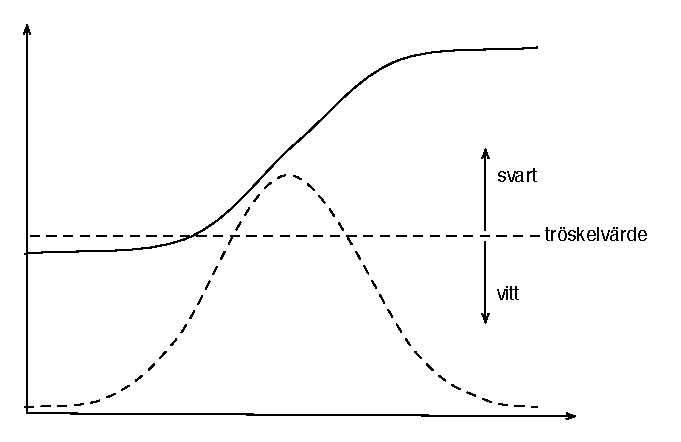
\includegraphics[width=\textwidth]{../img/w13-assignment-imageprocessing/derivatabild2.pdf}
\caption { En funktion (heldragen linje) och dess derivata (streckad linje).}
\label{fig:derivatabild}
\end{figure}

I figur~\ref{fig:derivatabild} visas en funktion $f$ (heldragen linje) och funktionens derivata $f'$ (streckad linje). Vi ser att där funktionen gör ett ''hopp'' så får derivatan ett stort värde. Om funktionen representerar intensiteten hos pixlarna längs en linje i x-led eller y-led så motsvarar ''hoppen'' en kontur i bilden. Om man sedan bestämmer sig för att pixlar där derivatans värde överstiger ett visst tröskelvärde ska vara svarta och andra pixlar vita så får man en bild med bara konturer. 

Nu är ju intensiteten hos pixlarna inte en kontinuerlig funktion som man kan derivera enligt vanliga matematiska regler. Men man kan approximera derivatan, till exempel med följande formel:

\begin{displaymath}
f'(x) \approx \frac{f(x+h) - f(x-h)}{2h}
\end{displaymath}

(Om man här låter $h$ gå mot noll så får man definitionen av derivatan.) Uttryckt i Scala och matrisen \code{intensity} så får man:

\begin{Code}
val derivative = (intensity(i)(j+1) - intensity(i)(j-1)) / 2
\end{Code}

Allt detta kan man uttrycka med hjälp av faltning. 

\begin{enumerate} 
	\item Beräkna intensitetsmatrisen med metoden \code{computeIntensity}.
	\item Falta varje punkt i intensitetsmatrisen med två kärnor:
$$
X\_SOBEL =
\begin{pmatrix}
  -1 & 0 & 1 \\
  -2 & 0 & 2 \\
  -1 & 0 & 1 \\
\end{pmatrix}
Y\_SOBEL =
\begin{pmatrix}
  -1 & -2 & -1 \\
  0 & 0 & 0 \\
  1 & 2 & 1 \\
\end{pmatrix}
$$
	Använd metoden \code{convolve} med vikten 1. Koefficienterna i matrisen $X\_SOBEL$ uttrycker derivering i x-led, i $Y\_SOBEL$ faltning i y-led. För att förklara varför koefficienterna ibland är 1 och ibland 2 måste man studera den bakomliggande teorin noggrant, men det gör vi inte här.
	\item Om resultaten av faltningen i en punkt betecknas med \code{sx} och \code{sy} så får man en indikator på närvaron av en kontur med \code{math.abs(sx) + math.abs(sy)}. Absolutbelopp behöver man eftersom man har negativa koefficienter i faltningsmatriserna. 
	\item  Sätt pixeln till svart om indikatorn är större än tröskelvärdet, till vit annars. Tröskelvärdet bestäms av \code{paramValue}. 
\end{enumerate}

Skriv en klass \code{SobelFilter} som implementerar denna algoritm.

\begin{figure}[H]
\begin{center}
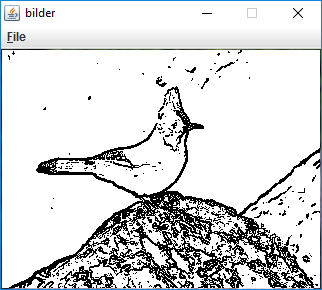
\includegraphics[scale=0.8]{../img/w13-assignment-imageprocessing/sobeljay.png}
\caption { Exempel på en bild där ett Sobelfilter applicerats med ett parametervärde på 150.}
\label{fig:sobel}
\end{center}
\end{figure}


\Task Implementera \code{FilterList} enligt specifikationerna ovan.

\Task Implementera \code{FilterChooser} enligt specifikationerna ovan.

\Task Knyt ihop allt i \code{ImageProcessing}-objektet som du skapade innan. Utskrifterna ska se ut på följande sätt:

{\setlength{\parindent}{0cm}

 Välj en av följande bilder genom att mata in en siffra\newline

0. boy.jpg\newline
1. car.jpg\newline
2. duck.jpg\newline
3. facade.jpg\newline
4. jay.jpg\newline
5. moon.jpg\newline
6. obidos.jpg\newline
7. sgrada.jpg\newline
8. shuttle.jpg\newline
Ditt val: 1\newline
Bild car.jpg laddad\newline
Tryck på 0 för Vanligt-filter\newline
Tryck på 1 för Blått-filter\newline
Tryck på 2 för Krypterat-filter\newline
Tryck på 3 för Inverterat-filter\newline
Tryck på 4 för Grått-filter\newline
Tryck på 5 för Kontrast-filter\newline
Tryck på 6 för Gauss-filter\newline
Tryck på 7 för Sobel-filter\newline
Tryck 42 om du inte vill använda fler filter\newline
Välj ett filter 1\newline
Välj ett filter 42\newline
Välja ny bild? (y/n) n\newline
}

Tänk på att användaren kan mata in otillåtna värden. Detta ska hanteras på lämpligt sätt.

\subsection{Frivilliga extrauppgifter}

\Task \textbf{Kontrastfilter.} Om man applicerar kontrastfiltrering på en färgbild så kommer bilden att konverteras till en gråskalebild. (Man kan naturligtvis förbättra kontrasten i en färgbild och få en färgbild som resultat. Då behandlar man de tre färgkanalerna var för sig.) Många bilder lider av alltför låg kontrast. Det beror på att bilden inte utnyttjar hela det tillgängliga området 0–255 för intensiteten. Man får en bild med bättre kontrast om man ''töjer ut'' intervallet enligt följande formel (lineär interpolation):

\begin{Code}
val newIntensity = 255 * (intensity - 45) / (225 - 45)
\end{Code}

Som synes kommer en punkt med intensiteten 45 att få den nya intensiteten 0 och en punkt med intensiteten 225 att få den nya intensiteten 255. Mellanliggande punkter sprids ut jämnt över intervallet \code{[0, 255]}. För punkter med en intensitet mindre än 45 sätter man den nya intensiteten till 0, för punkter med en intensitet större än 225 sätter man den nya intensiteten till 255. Vi kallar intervallet där de flesta pixlarna finns för \code{[lowCut, highCut]}. De punkter som har intensitet mindre än \code{lowCut} sätter man till 0, de som har intensitet större än \code{highCut} sätter man till 255. För de övriga punkterna interpolerar man med formeln ovan (45 ersätts med \code{lowCut}, 225 med \code{highCut}).

Det återstår nu att hitta lämpliga värden på \code{lowCut} och \code{highCut}. Detta är inte något som kan göras helt automatiskt, eftersom värdena beror på intensitetsfördelningen hos bildpunkterna. Man börjar med att beräkna bildens intensitetshistogram, dvs hur många punkter i bilden som har intensiteten 0, hur många som har intensiteten 1, . . . , till och med 255.

I de flesta bildbehandlingsprogram kan man sedan titta på histogrammet och interaktivt bestämma värdena på \code{lowCut} och \code{highCut}. Så ska vi dock inte göra här. I stället bestämmer vi oss för ett procenttal \code{cutOff} (som bestäms av \code{paramValue}) och beräknar \code{lowCut} så att \code{cutOff} procent av punkterna i bilden har en intensitet som är mindre än \code{lowCut} och \code{highCut} så att \code{cutOff} procent av punkterna har en intensitet som är större än \code{highCut}.

Exempel: antag att en bild innehåller 100 000 pixlar och att \code{cutOff} är 1.5. Beräkna bildens intensitetshistogram i en vektor
\begin{Code} 
val histogram = Array[Int](256)
\end{Code}

Beräkna \code{lowCut} så att \code{histogram(0)} + ... + \code{histogram(lowCut)} = 0.015 * 100000 (så nära det går att komma, det blir troligen inte exakt likhet). Beräkna \code{highCut} på liknande sätt.

Sammanfattning av algoritmen:
\begin{enumerate}
	\item Beräkna intensiteten hos alla punkterna i bilden, lagra dem i en \code{short}-matris. Använd den färdigskrivna metoden \code{computeIntensity}.
	\item Beräkna bildens intensitetshistogram.
	\item Parametervärdet \code{paramValue} är det värde som ska användas som \code{cutOff}.
	\item Beräkna \code{lowCut} och \code{highCut} enligt ovan.
	\item Beräkna den nya intensiteten för varje pixel enligt interpolationsformeln och lagra de nya pixlarna i \code{outPixels}.
\end{enumerate}
Skriv en klass \code{ContrastFilter} som implementerar algoritmen. I katalogen \emph{images} kan bilden \emph{moon.jpg} vara lämpliga att testa, eftersom den har låg kontrast. Anmärkning: om \code{cutOff} sätts = 0 så får man samma resultat av denna filtrering som man får av \code{GrayScaleFilter}. Detta kan man se genom att studera interpolationsformeln.

%%!TEX encoding = UTF-8 Unicode

%!TEX root = ../compendium2.tex

%!TEX encoding = UTF-8 Unicode
\chapter{Muntlig examen}\label{chapter:W14}


%!TEX encoding = UTF-8 Unicode
%!TEX root = ../lect-week14.tex

%%%

\Subsection{Tentatips}
\begin{Slide}{Före tentan:}\SlideFontSmall
\begin{enumerate}
\item Repetera övningar och labbar i kompendiet. 
\item Läs igenom föreläsningsanteckningar.
\item Studera \Emph{snabbref} \Alert{mycket noga} så att du vet vad som är givet och var det står, så att du kan hitta det du behöver snabbt.
\item Skapa och \Emph{memorera} en personlig \Emph{checklista} med programmeringsfel du brukar göra, som även inkluderar småfel, så som glömda parenteser och semikolon, och annat som en kompilator/IDE normalt hittar.
\item Tänk igenom hur du ska disponera dina 5 timmar på tentan.
\item Gör den minst en extenta som om det vore \Alert{skarpt läge}: 
\begin{enumerate}\SlideFontTiny
\item Avsätt 5 ostörda timmar (stäng av telefon, dator etc).
\item Inga hjälpmedel. Bara snabbref.
\item Förbered dryck och tilltugg.
\end{enumerate}
\end{enumerate}
\end{Slide}

\begin{Slide}{På tentan:} \SlideFontTiny
\begin{enumerate}
\item Läs igenom \Alert{hela} tentan först. \\ \Emph{Varför?} Förstå helheten. Delarna hänger ihop.
\item Notera och begrunda specifika begrepp och definitioner. \\ \Emph{Varför?} Begreppen är avgörande för förståelsen av uppgiften.
\item Notera förenklingar, antaganden och specialfall. \\ \Emph{Varför?} Uppgiften blir mkt enklare om du inte behöver hantera dessa.
\item \Alert{Fråga} tentamensansvarig om du inte förstår uppgiften -- speciellt om det finns misstänkta felaktigheter eller förmodat oavsiktliga oklarheter. \\ \Emph{Varför?} Det är inte lätt att konstruera en ''perfekt'' tenta. \\ Du får fråga vad du vill, men det är inte säkert du får svar :)
\item Läs specifikationskommentarerna och metodsignaturerna i alla givna klass-specifikationer \Alert{mycket noga}. \\ \Emph{Varför?} Det är ett vanligt misstag att förbise de ledtrådar som ges där.
\item Återskapa din memorerade personliga checklista för vanliga fel som du brukar göra och avsätt tid till att gå igenom den på tentan. Varje fix plockar poäng!
\item Lämna in ett försök även om du vet att lösningen inte är fullständig. Det gäller att ''plocka poäng'' på så mycket som möjligt. En dålig lösning kan ändå ge poäng.

\item Om du har svårigheter kan det bli kamp mot klockan. Försök hålla huvudet kallt och prioritera utifrån var du kan plocka flest poäng. Ge inte upp! Ta en kort äta-dricka-paus för att få mer energi!

\end{enumerate}
\end{Slide}

\ifkompendium\else

\begin{Slide}{Planeringstips}\SlideFontTiny
Exempel på saker som du kan lägga in tid för i din julpluggkalender:
\begin{enumerate}
\item Välja ut övningar att repetera
\item Repetera övning X, Y, Z, ... Både läsa och skriva kod. Fundera på typ och värde.
\item Välja ut labbar att repetera
\item Repetera labb X, Y, Z, ... Lär dig ''trick'' och ''mönster''.
\item Träna på att skriva program med papper och penna
\item Göra checklista med vanliga fel
\item Läsa igenom extentor i Java
\item Välja ut minst en Java-extenta att göra som i skarpt läge i Scala
\item Gör Java-extentor X, Y, Z, ... implementera (delar) i Scala
\item Gör utvalda delar av extenta X, Y, Z, ... i Java
\end{enumerate}
\end{Slide}

\Subsection{Avgränsning}

\begin{Slide}{Tentans struktur}
\begin{itemize}
\item Del A 20\%:\\\Emph{Läsa uttryck} där du ska \Alert{ange typ och värde}
\begin{itemize}\SlideFontTiny
\item Du kommer att behöva skriva ner delsteg och variablers värden (minnet)
\item Testar förståelse av variabler, uttryck, samlingar, algoritmer, arv, etc.
\item Uppdaterad (mildare) regel om ''rättningströskel'': \\
Ur senaste compendium.pdf kapitel 0.8: \textit{Om du på del A erhåller färre poäng än vad som krävs för att nå upp till en bestämd ''rättningströskel'', kan din tentamen komma att underkännas utan att del B bedöms.}
\item Liknar kompendiets övningar; rimlig att lösa och dubbelkolla på 1h
\end{itemize}


\item Del B 80\%:\\\Emph{Skriva kod} som uppfyller \Alert{krav och designspecifikation}
\begin{itemize}\SlideFontTiny
\item Testar att du själv kan skapa kod med delar som samverkar
\item Testar förmåga att gå från indata-utdata till algoritm \\
 givet: ledtrådar, design, ev. skiss på lösning, ev. pseudokod etc.
\item Liknar kompendiets labbar; rimlig att lösa och dubbelkolla på 4h 
\end{itemize}

\end{itemize}
\end{Slide}



\begin{Slide}{Vad kommer på tentan? (1 av 3)}\SlideFontTiny
\hspace{-1em}\begin{minipage}{1.0\textwidth}
Allmänt: 
\begin{itemize}\SlideFontTiny
\item Begrepp som är ''fördjupning'' krävs ej på tentan (men ökar förståelse)
\item Ok om du väljer en enklare lösning med basala begrepp som fungerar bra, \\i stället för en kortare/elegantare/mer avancerad lösning
\item Dessa moduler ingår ej på tentan: ''Trådar, webb'', ''Design, api''
\end{itemize}

\vspace{1em}\begin{tabular}{l | l | l}
\textbf{Modul} & \textit{Ingår t.ex.}& \textit{Avgränsning} (ej krav; ok anv. om lämpl.)\\\hline
Introduktion & uttryck, aritmetik, slumptal, & kan ha nytta av deMorgan men ej krav\\
             & strängar, typer, Unit   & skriva egna \code|s"$x"| (men kunna läsa)  \\
             & skillnad mellan heltal \& flyttal & Float, Byte, Short\\
             & variabler, for, while, if & hex-literaler, backticks\\ 
\hline
Kodstrukturer & iterering, SWAP, SUM, MIN/MAX & import, paketnamn\\             
              & loopar, Range, sats vs uttryck & ok att välja vilken loop du tycker passar\\
              & namn, synlighet, skuggning & scaladoc, javadoc, jar \\        
\hline
Funtioner,    & definiera, anropa, parameter& skapa egen kontrollstruktur\\
objekt        & returtyp, namnarop, defaultarg & stegad funktion, rekursion\\        
              & punktnotation, objekt vs static & lazy val\\        
              & map/foreach med egen funktion & \\
              & anonyma funktioner (lambda)  & \\                              

\end{tabular}
\end{minipage}
\end{Slide}


\begin{Slide}{Vad kommer på tentan? (2 av 3)}\SlideFontTiny
\hspace{-2em}\begin{minipage}{1.0\textwidth}
\begin{tabular}{l | l | l}
\textbf{Modul} & \textit{Ingår t.ex.}& \textit{Avgränsning} (ej krav; ok anv. om lämpl.)\\\hline
Datastrukt. & attribut, medlem, metod, klass & isInstanceOf (anv. match istället) \\
            & tupler, Vector, Set, Map & List (oftast Vector istället)\\
            & Source.fromFile          & java.nio.file \\
\hline
Sekvensalg. &  skapa ny samling från befintlig &  \\      
            &  registrering, Scanner, ArrayBuffer & StringBuilder\\
            &  uppdatera Array, ArrayBuffer, Vector & \\
            &  slumptalsfrö, scala.util.Random  &  \\
\hline

Klasser     &  new, this, synlighet  & null \\
            &  inkapsling, accessregler, private  & private[this] \\
            &  klassparameter, fabriksmetod  & \\
            &  class vs case class    & \\
            &  referenslikhet vs innehållslikhet    & \\
            &  föränderlig vs oföränderlig klass & \\
\hline
Arv         &  bastyp, subtyp, trait, extends  & \\
            &  överskuggning,                  & inmixning, \\
            &  Any, AnyVal, AnyRef, Object     & Null, Nothing\\
            &  accessregler vid arv, protected & final\\
            &  abstract class, case object     & \\
            
\end{tabular}
\end{minipage}
\end{Slide}


\begin{Slide}{Vad kommer på tentan? (3 av 3)}\SlideFontTiny
\hspace{-2em}\begin{minipage}{1.0\textwidth}
\begin{tabular}{l | l | l}
\textbf{Modul} & \textit{Ingår t.ex.}& \textit{Avgränsning} (ej krav; ok anv. om lämpl.)\\\hline

Mönster     & match, Option, Try & try catch, unapply\\
            & flatten, sealed            & flatMap, partiella funktioner\\
            & enkel equals utan arv     & hashcode, fullständig equals   \\ 
            & wildcard-mönster  & variabelbindn. i mönster, sekvensmönster\\
\hline

Matriser,     & indexering i nästlade strukturer & \\
typparametrar & nästlad for-sats  & \\ 
              & matriser i Java med array  & \\
              & använda generiska strukturer & skapa generiska strukturer\\ 
\hline

Sök, sortera & linjärsökning, binärsökning & algoritmisk komplexitet\\
            & compareTo, strängjämförelse & Ordering, Ordered\\
            & insättningssortering & räcker kunna en valfri sortering \\
\hline


Scala/Java & översätta enkel Java/Scala & try catch i Java \\
           & implemenetera Java-klass     &  arv i Java med super vid konstr.\\
           & grundläggande syntaxskillnader & \\
           & ArrayList vs ArrayBuffer & java.util.\{List, Set\}\\
           & Autoboxing vid ArrayList<Integer> & \\
\multicolumn{3}{c}{OBS! Java-övningar finns även här och där i andra moduler}\\
\hline           
     
\end{tabular}
\end{minipage}
\end{Slide}


\Subsection{Tips vid val av lösningar}


\begin{Slide}{Tips om val av klass/trait}\SlideFontSmall
Ofta ger tentan en specifik design, men du kan ha stor nytta av egna abstraktioner, speciellt \Emph{lokala funktioner} för att göra enklare dellösningar!

\pause\vspace{1em}Om du skulle behöva samla både attribut och metoder utöver givan specifikationer:
Singelobjekt, case-klass, klass, trait eller abstrakt klass?
\begin{itemize}\SlideFontTiny
\item Använd \code{object} om du behöver samla metoder (och variabler) i en modul som bara finns i en upplaga. Du får lokal namnrymd och punktnotation på köpet.
\item Använd en \code{case class} om du har \Emph{oföränderlig data}. Du får då även innehållslikhet, möjlighet till mönstermatchning, etc. på köpet! 
\item Behöver du \Alert{föränderligt tillstånd} använd en vanlig \code{class}.\\ Det normala är att tillståndet (alla attribut) är \code{private} eller \code{protected} och att all uppdatering och avläsning av tillståndet sker indirekt genom metoder (getters/setters/...). 
\item Behöver du en abstrakt bastyp utan konstruktorparametrar använd en \code{trait}. \\(Du får inmixningsmöjlighet med \code{with} på köpet. Inmixning kommer ej på tenta.)
\item Behöver du en abstrakt bastyp med konstruktorparametrar använd en \code{abstract class}. (Går dock ej att använda vid inmixning med \code{with}.)
\end{itemize}
\end{Slide}


\begin{Slide}{Tips om hur man läser en specifikation}\SlideFontSmall
När du läser en specifikation av en klass, en trait, eller ett singelobjekt:
\begin{itemize}
\item Tänk igenom vilket ansvar olika delar av koden har
\item Vad håller klassen reda på? \\$\rightarrow$ Ledtrådar till attribut
\item Vad ska klassen göra/räkna ut? \\$\rightarrow$ Ledtrådar till metoder och deras algoritm
\item Vilka andra klasser har nytta av denna metod? \\$\rightarrow$ Ledtrådar till hur klasserna samverkar för att lösa uppgiften
\end{itemize}
Rita gärna en bild med ett specifikt exempel på vilken data som olika instanser håller reda på och fundera på hur data skapas/beräknas/förändras
\end{Slide}


\begin{Slide}{Tips om val av samling}\SlideFontSmall

Generellt: Det är ofta enklare med oföränderliga samlingar med oföränderliga element och skapa nya samlingar vid förändring. Men ibland blir det enklare om man har föränderliga samlingar.

\begin{itemize}
\item Behöver du hantera värden \code{x} av t.ex. typen String med \Emph{heltalsindex}?
\begin{itemize}\SlideFontTiny
\item Om du klarar dig utan förändring av innehållet:\\ \code{ val xs: Vector[String]}
\item Om du behöver ändra innehåll men \Alert{inte} antal element: \\ \code{ val xs: Array[String]} 
\item Om du behöver ändra innehåll \Alert{och} antal element: 
\\ \code{ var xs: Vector[String] } (se metoden \code{patch}) eller \\ \code{ val xs: ArrayBuffer[String]} (har metoden \code{insert})
\end{itemize}

\item Behöver du hantera värden \code{x} som ska vara unika?
\begin{itemize}\SlideFontTiny
\item Oföränderlig: \code{  val xs: Set[String] }
\item Förändringsbar: \code{val xs: scala.collection.mutable.Set[String]}
\end{itemize}

\item Behöver du leta upp värden \code{x:Int} utifrån en nyckel av t.ex. String?
\begin{itemize}\SlideFontTiny
\item Oföränderlig: \code{   val xs: Map[String, Int] }
\item Förändringsbar: \code{val xs: scala.collection.mutable.Map[String, Int]}
\end{itemize}


\end{itemize}
\end{Slide}

\begin{Slide}{Tillåtna uppdateringar i din QuickRef}
Du får med egen penna göra dessa fixar i din QuickRef:
\begin{itemize}
\item Grundtypernas implementation, sid 4: 
\begin{itemize}

\item omfång för Int ska ha exponent 31 (inte 15), 
\item omfång för Long ska ha exponent 63 (inte 15).
\end{itemize}

\item Saknade samlingsmetoder: 
\begin{itemize}
\item Under rubriken "Methods in trait Map[K, V]" saknas metoderna keySet och mapValues. 
\item Saknade metoderna för mutable.ArrayBuffer[T]: \\ \code{update} \code{insert} \code{remove} \code{append} \code{prepend}, etc. \\ lägg till beskrivning på lediga platsen på sista sidan \\ 
(se vidare commit \href{https://github.com/lunduniversity/introprog/commit/a5e29d000062}{a5e29d000062a} i kursrepot)
\end{itemize}
\end{itemize}
\end{Slide}


\begin{Slide}{ArrayBuffer}
Viktigast att känna till: update, insert, remove, append
{\SlideFontTiny

\vspace{2.5em}\begin{tabular}{@{}p{4.2cm}  p{6.5cm}}
\texttt{xs(i) = x \newline xs.update(i, x)} & Replace element at index i with x. \newline Return type Unit.\\   \cline{1-2}

\texttt{xs.insert(i, x)\newline xs.remove(i)} & Insert x at index \texttt{i}. Remove element at i. \newline Return type Unit.\\   \cline{1-2}

\texttt{xs.append(x)~~~xs~+=~x} & Insert x at end.  Return type Unit.\\   \cline{1-2}

\texttt{xs.prepend(x)~~x~+=:~xs} & Insert x in front.  Return type Unit.\\   \cline{1-2}

\texttt{xs -= x} & Remove first occurance of x (if exists). \newline Returns xs itself. \\\cline{1-2}

\texttt{xs ++= ys} & Appends all elements in ys to xs and returns xs itself. \\

\end{tabular}
}
\end{Slide}



\Subsection{Genomgång av extenta}
\begin{Slide}{Extenta 2016-08-24 TimePlanner}\SlideFontSmall
\url{http://cs.lth.se/pgk/examination/}

\vspace{1em}\Alert{TimePlanner}: 
\begin{itemize}
\item \href{http://fileadmin.cs.lth.se/cs//Education/grundkurs/extentor/160824.pdf}{tentamen 160824} 
\item \href{http://fileadmin.cs.lth.se/cs//Education/grundkurs/extentor/sol-160824.pdf}{lösningsförslag Java} 
\item \href{https://github.com/lunduniversity/introprog/tree/master/compendium/examples/exam/re-impl-java-exams/timeplanner-160824}{översättning av lösning till Scala}
\end{itemize}
\end{Slide}


\Subsection{Avslutning av kursen}

\begin{Slide}{Obligatoriska moment}\SlideFontSmall
\begin{itemize}
\item Kolla vilka oblikatoriska moment du har kvar här:
\url{http://fileadmin.cs.lth.se/pgk/SAM-EDAA45-snapshot.html}
\item Sök på din födelsemånad/dag, tex 0102 för andra Januari.
\item Läs \Alert{alla} instruktioner \Alert{noga} och \Alert{anmäl dig} här: \\
\href{http://www.student.lth.se/studieinformation/anonyma-tentor/}{www.student.lth.se/studieinformation/anonyma-tentor}
\item Du ska vara godkänd på alla labbar+projekt för att få tenta pgk EDAA45!
\item Du ska vara godkänd på alla labbar+projekt för att få gå pfk \href{http://cs.lth.se/edaa01vt}{EDAA01}!
\item Använd återstående \Emph{resurstider} för \Alert{redovisning av labbar/projekt}.
\end{itemize}
\end{Slide}

\begin{Slide}{CEQ -- Course Experience Questionnaire}\SlideFontSmall
\begin{itemize}
\item Görs på hela LTH på samma sätt. Alla får länkar via mejl.
\item Snälla fyll i CEQ! Jag är \Alert{mycket tacksam} för all konstruktiv feedback! \\ Hög svarsfrekvens är viktigt för att kunna dra slutsatser om variationen i svaren och signifikansen i sammanställningen.
\item Del 1: Generella påståenden, alla med 5-gradig skala: \\ tar helt avstånd ... instämmer helt
\item Del 2: \Emph{Fritextfrågor}: \\
''Vad  tycker  du  var  det  bästa  med  den här  kursen?'' \\
''Vad  tycker  du  främst  behöver  förbättras?''
\item Fördel med CEQ: Samma alla kurser alla år medger jämförelse över tid.
\item Begränsning med CEQ: Saknar frågor kopplat till specifika kursmoment.
\item Mer om CEQ här: \url{https://www.ceq.lth.se/}
\end{itemize}
\end{Slide}

\begin{Slide}{Kursspecifik utvärdering om specifika kursmoment}\SlideFontSmall
\begin{itemize}
\item Jag vill gärna att alla gör den LTH-gemensamma, anonyma kursutvärderingsenkäten \href{https://www.ceq.lth.se/}{CEQ}. Dina fritext-kommentarer om vad som är det bästa med kursen och vad som främst behöver förbättra emottages mycket tacksamt i CEQ-utvärderingen!
\item Jag kommer att komplettera CEQ med en \Emph{kursspecifik} utvärdering av specifika kursmoment i denna kurs och jag är därför \Alert{mycket tacksam} om alla fyller enkäten när länk kommer via mejl. 
\item Jag behandlar dina svar konfidentiellt, men ber om din STiL-id så att jag kan återkomma om jag mot förmodan undrar något mer.
\item Din input är mycket värdefull vid framtida kursutveckling!
\end{itemize}
\end{Slide}

\begin{Slide}{Intresserad av att arbeta som handledare?}
\begin{itemize}
\item Vi har ständigt behov av nya handledare i våra kurser
\item Det är lärorikt att jobba som timanställd handledare
\item Kontakta \verb|bjorn.regnell@cs.lth.se| eller annan kursansvarig i den kurs du vill jobba
\end{itemize}
\end{Slide}

\begin{Slide}{Utblick}\SlideFontSmall
Några framtida \Emph{kurser} som direkt bygger på pgk:
\begin{itemize}
\item Fördjupningskursen (Java)
\item Utvärdering av programvarusystem (R)
\item Diskreta strukturer (Clojure)
\item Programvaruutveckling i grupp 
\item Objekt-orienterad modellering och design
\item Funktionsprogrammering 
\end{itemize}
Framtiden för \Emph{Scala}:
\begin{itemize}
\item Scala 2.12 bättre bytekod, Scala 2.13 bättre standardbibliotek
\item Ny kompilator: \Emph{dotty}; Nytt format ''över'' bytekod: \Emph{Tasty}
\item Scala.JS: dela kod+kompetens mellan backend och frontend
\item Scala native: kör Scala kompilerat direkt ''på metallen''
\item Scala-ramverk för stordata, massiv parallellism, AI, ...
\end{itemize}
\end{Slide}

\begin{Slide}{Hoppas att kursen varit kul och lärorik!}

\includegraphics[width=5cm]{../img/gurka.jpg}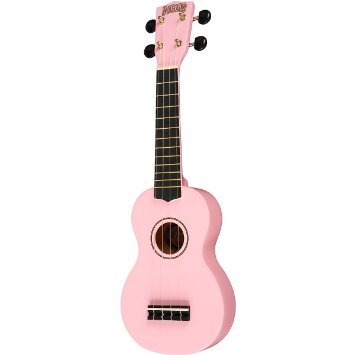
\includegraphics[width=5cm]{../img/ukulele.jpg}
\end{Slide}

\begin{Slide}{Ett stort TACK för...}
\begin{itemize}
\item ... att ni kämpat så hårt!
\item ... att ni ställt massor med frågor!
\item ... att det har varit så hög närvaro på föreläsningarna!
\item ... att ni är så konstruktiva och verkligen vill lära er!
\end{itemize}
\vspace{2em} \pause

\Alert{Ett stort LYCKA TILL på vägen till att bli en \\ kompetent och innovativ systemutvecklare!}
\end{Slide}


\fi



%\part{Appendix}
%\appendix
%%!TEX encoding = UTF-8 Unicode
%!TEX root = ../compendium2.tex

\chapter{Terminalfönster}\label{appendix:terminal}

\section{Vad är ett terminalfönster?}

I ett terminalfönster kan man skriva kommandon som kör program och hanterar filer. När man programmerar använder man ofta terminalkommando för att kompilera och exekvera sina program.  
 
\subsubsection{Terminal i Linux}

    \begin{figure}[!b]
    \centering
    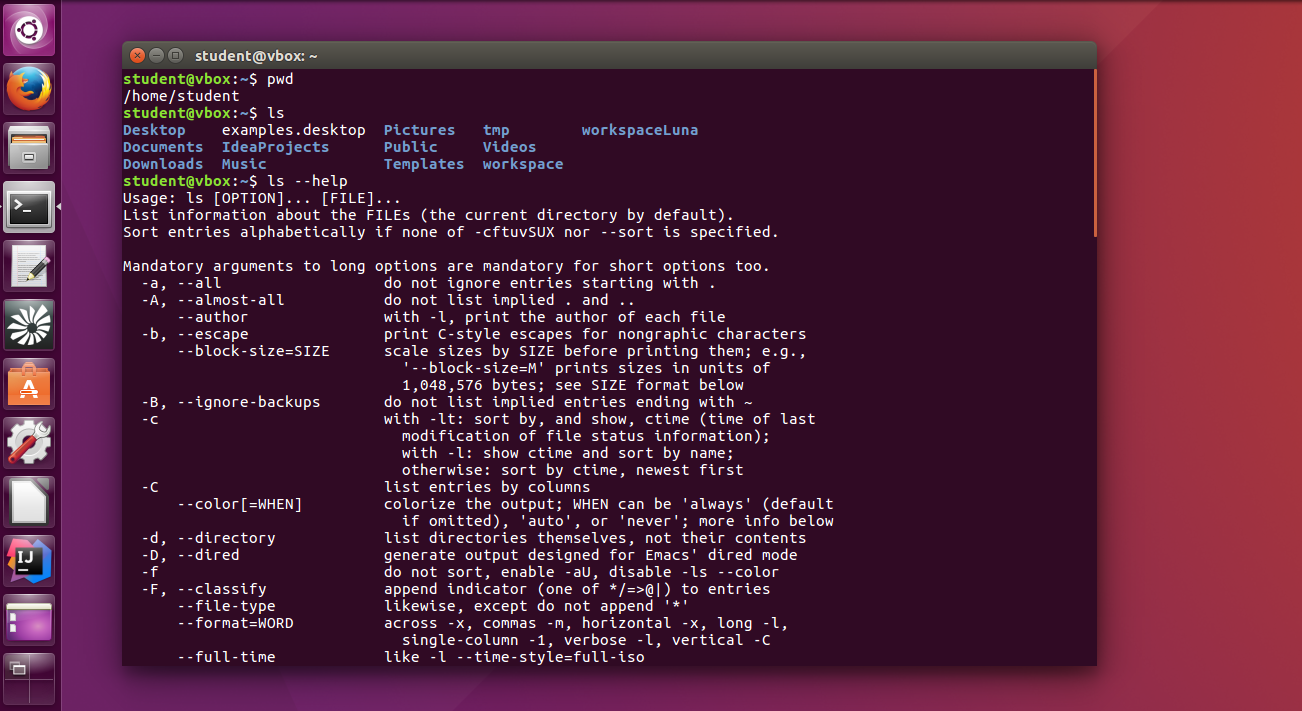
\includegraphics[width=1.0\textwidth]{../img/linux-terminal.png}
    \caption{Terminalfönster i Ubuntu öppnas med Ctrl+Alt+T.}
    \label{fig:terminal:linux}
    \end{figure}

I Ubuntu trycker du lättast \textbf{Ctrl+Alt+T} eller sök efter ''terminal'' i app-menyn.  Då öppnas ett fönster med en blinkande markör som visar att det är redo att ta emot dina textkommando. Ett exempel på kommando är \texttt{ls} som skriver ut en lista med filer i det aktuella biblioteket, så som visas i fig. \ref{fig:terminal:linux}.

Det som visas i ett terminalfönster sköts av ett \textbf{kommandoskal} \Eng{command shell}, som är redo att ta emot kommando efter en prompt som slutar med ett \texttt{\$}-tecken. När du skriver ett kommando och trycker Enter anropar kommandoskalet en kommandotolk som tolkar och utför dina kommandon. Om ett kommando inte kan tolkas, skrivs ett felmeddelande. 

Det finns många användbara kortkommando, varav de viktigaste visas i tabell \ref{fig:terminal:shortcuts}. Det är bra om du lär dig dessa kortkommandon utantill så att ditt arbete i terminalen går snabbt och smidigt.

\begin{table}[H]
\renewcommand{\arraystretch}{1.15}
\begin{tabular}{@{}r | l}
pil upp/ner & bläddra i kommandohistoriken \\
Tab & ''auto-complete'', fyll i resten baserat på vad du skrivit hittills \\
Tab Tab & två tryck på Tab listar flera alternativ, om så finnes \\
Ctrl+A & ''ahead'', flytta markören till början av raden \\
Ctrl+E & ''end'', flytta markören till slutet av raden \\
Ctrl+K & ''kill'', ta bort tecken från markören till radens slut\\
Ctrl+U & ''undo'', ta bort tecken från markören till början av raden \\
Ctrl+Y & ''yank'', sätt in det som senast togs bort\\
Ctrl+Z & ''zleep'', stoppa pågående process, skriv sedan \texttt{bg} för bakgrundskörning\\
Ctrl+L & rensa terminalfönstret\\
Ctrl+D & avsluta kommandoskalet \\
\end{tabular}
    \caption{Viktiga kortkommandon i Linux terminalfönster.}
    \label{fig:terminal:shortcuts}
\end{table}

\noindent Ctrl+C orsakar normalt ett avbrott av pågående process, men om du vill att Ctrl+C ska vara ''Copy'' som vanligt för att kopiera markerad text, kan du ställa om detta med terminalförnstrets  meny ''Edit $\rightarrow$ Keyboard Shortcuts'', eller liknande.




 
\subsubsection{PowerShell, Cmd och Linux i Microsoft Windows}
Microsoft Windows är inte Linux-baserat, men i kommandotolken \textbf{Powershell} finns alias definierade för några vanliga Linux-kommandon, inkluderat \texttt{ls}, \texttt{cd} och \texttt{pwd}. 
Du startar Powershell t.ex. genom att trycka på Windows-knappen och skriva \texttt{powershell}. 
Du kan också, medan du bläddrar bland filer, klicka på filnamnsraden överst i filbläddraren och skriva \texttt{powershell} och tryck Enter; då startas Powershell i aktuellt bibliotek. Ändra gärna typsnitt och bakgrundsfärg med hjälp av fönstrets menyer, så att det blir lättare för dig att läsa vad som skrivs.

Det finns även i Windows den ursprungliga kommandotolken \textbf{Cmd} med helt andra kommandon. Till exempel skriver man i Cmd kommandot \texttt{dir} i stället för \texttt{ls} för att lista filer. 

I Windows 10 kan du (numera, om du installerad senaste uppdateringarna av Windows) även köra Ubuntu-terminalen med hjälp av Windows Linux Subsystem (WSL). Se vidare här om hur du kan installera WSL under Windows 10: 

\url{https://ubuntu.com/wsl} 

Läs mer här: \href{https://www.omgubuntu.co.uk/2020/03/windows-10-linux-kernel-update}{www.omgubuntu.co.uk/2020/03/windows-10-linux-kernel-update}



\subsubsection{Terminal i Apple macOS/OS X}


Apple OS X och macOS är Unix-baserade operativsystem. De flesta vanliga terminalkommandon som fungerar i Linux fungerar också under Apple OS X och macOS. Du startar ett terminalfönster i Apples operativsystem genom att klicka på förstoringsglaset uppe till höger, skriva \texttt{terminal}, och trycka Enter.

\section{Vad är en path/sökväg?}\label{terminal:path}

När du skriver ett kommando i terminalen, eller kör vilket program som helst på din dator, behöver operativsystemet identifera i vilken fil programmets maskinkod ligger innan programmet kan köras. 

Lokaliseringen av filer sker med hjälp av en \textbf{sökväg} \Eng{path}, som anger en position i filsystemet. Ofta betraktas filsystemet som ett upp-och-ned-vänt träd, och kallas därför även ''filträdet''. Den ''översta'' positionen kallas ''rot'' \Eng{root} och betecknas med ett enkelt snedstreck \texttt{/}. Kataloger som ligger i kataloger utgör förgreningar i trädet. En sökväg pekar ut vägar genom trädet som behövs för att nå ''löven'', som utgörs av själva filerna.

Du kan se var ett program ligger i Linux med hjälp av kommandot \texttt{which} enligt nedan.\footnote{Skriv \texttt{ gcm ls } i Windows Powershell för motsvarighet till \texttt{ which ls } \\ Eller skriv \texttt{ New-Alias which get-command } för tillgång till kommandot \texttt{which} i Powershell. \\ \href{http://stackoverflow.com/questions/63805/equivalent-of-nix-which-command-in-powershell}{stackoverflow.com/questions/63805/equivalent-of-nix-which-command-in-powershell}} Listan med bibliotek i sökvägen avskiljs med snedstreck.
\begin{REPLnonum}
$ which java
/usr/lib/jvm/oracle_jdk8/bin/java
$ which ls
/bin/ls
\end{REPLnonum}

En sökväg kan vara \textbf{absolut} eller \textbf{relativ}. En absolut sökväg utgår från roten och visar hela vägen från rot till destination, t.ex. \texttt{/usr/bin/firefox}, medan en relativ sökväg utgår från aktuellt bibliotek (där du ''står'') och börjar \textit{inte} med ett snedstreck.

Alla operativsystem håller reda på en mängd olika sökvägar för att kunna hitta speciella filer i filträdet. Dessa sökvägar lagras i s.k. \textbf{miljövariabler} \Eng{environment variables}. Det finns en \textit{speciell} miljövariabel som heter kort och gott \textbf{PATH}, i vilken alla sökvägar till de program finns, som ska vara tillgängliga för din användaridentitet direkt för exekvering genom sina filnamn, \textit{utan} att man behöver ange absoluta sökvägar. 

Du kan i Linux se vad som ligger i din PATH med kommandot \code{ echo $PATH } medan man i Windows Powershell skriver \code{$env.Path} där det bara är första bokstaven som ska vara en versal. I Linux separeras biblioteken i sökvägen med kolon, medan Windows använder semikolon.

Ibland kan du behöva uppdatera din PATH för att program som du installerat och ska bli allmänt tillgängliga. Detta görs på lite olika sätt i olika operativsystem, för Linux se t.ex. här:
\href{http://stackoverflow.com/questions/14637979/how-to-permanently-set-path-on-linux}{stackoverflow.com/questions/14637979/how-to-permanently-set-path-on-linux}

När man anger sökvägar finns några tecken med speciell betydelse:

\begin{tabular}{r  p{0.8\textwidth}}
\code|~| & ''tilde'', din hemkatalog \\
\code|/| & ''slash'', snedstreck anger filträdets rot om det finns i början av sökvägen, men utgör biblioteksavskiljare inuti sökvägen \\
\code|.| & en punkt anger aktuellt bibliotek, där du ''står'' \\
\code|..| & två punkter anger ett steg ''upp'' i filträdet \\
\code|"| & omgärda en sökväg med citationstecken, först och sist, om den innehåller annat än engelska bokstäver, t.ex. blanktecken\\
\code|\ | & \textit{backslash+blanktecken} används för att beteckna mellanslag i sökvägar som \textit{inte} omgärdas av citationstecken\\
\end{tabular}

\section{Några viktiga terminalkommando}

I tabell \ref{fig:terminal:commands} finns en lista med några viktiga terminalkommando som är bra att lära sig utantill.

En introduktion till LTH:s datorer med exempel på hur du använder vanliga Linux-kommandon finns i denna skrift \url{http://www.ddg.lth.se/perf/unix/} som används i introduktionsveckan för nybörjare på datateknikprogrammet vid LTH.

På sajten \url{http://ss64.com/} finns en mer omfattande lista med användbara terminalkommando och tillhörande förklaringarför för Linux (Bash), Windows (Powershell, Cmd) och Apple OS X (Bash).  

\begin{table}[H]
\renewcommand{\arraystretch}{1.25}
   
\begin{tabular}{@{}r | l}
\texttt{ls} & lista filer i aktuellt bibliotek (alltså där du ''står'')\\
\texttt{ls} \textit{p}  & lista filer i biblioteket  \textit{p} \\
\texttt{ls -A} & lista alla filer i aktuellt bibliotek, även gömda \\
\texttt{man ls} & manual för kommandot \texttt{ls}; testa även \texttt{man} för andra kommandon! \\
\texttt{cd} \textit{p} & ''change directory'', ändra aktuellt bibliotek till \textit{p}\\
\texttt{pwd} & ''print working directory'', skriv ut sökväg för aktuellt bibliotek \\
\texttt{cp} \textit{p1 p2} & ''copy'', kopiera filen med path \textit{p1} till en ny fil kallad \textit{p2} \\
\texttt{mv} \textit{p1 p2} & ''move'', byt namn på filen \textit{p1} till \textit{p2}  \\
\texttt{rm} \textit{p} & ''remove'', ta bort filen \textit{p}\\
\texttt{rm -r} \textit{p} & ''remove recursive'', ta bort biblioteket \textit{p} med allt innehåll; var försiktig!\\
\texttt{mkdir} \textit{p} & ''make dir'', skapa ett nytt bibliotek \textit{p}\\
\texttt{cat} \textit{p1 p2}& ''concatenate'', skriv ut hela innehållet i en eller flera filer \textit{p1 p2 etc.}\\
\texttt{less} \textit{p}& skriv ut innehållet i filen \textit{p}, en skärm i taget\\
\texttt{wget} \textit{url}&ladda ner \textit{url}, t.ex. \texttt{ wget http://cs.lth.se/pgk/ws -o ws.zip}\\
\texttt{unzip} \textit{p}& packa upp \textit{p}, t.ex. \texttt{ unzip ws.zip}\\
\end{tabular}

    \caption{Några viktiga terminalkommando i Linux. Med \textit{p}, \textit{p1}, \textit{p2}, etc.  avses en absolut eller relativ sökväg \Eng{path}, se avsnitt \ref{terminal:path}.}
    \label{fig:terminal:commands}

\end{table}


%%!TEX encoding = UTF-8 Unicode
%!TEX root = ../compendium.tex

\chapter{Editera}\label{appendix:edit}
\section{Vad är en editor?}

En editor används för att redigera programkod. Det finns många olika editorer att välja på. Erfarna utvecklare lägger ofta mycket energi på att lära sig att använda favoriteditorns kortkommandon och specialfunktioner, eftersom detta påverkar stort hur snabbt kodredigeringen kan göras. 

En bra editor har \textbf{syntaxfärgning} för språket du använder, så att olika delar av koden visas i olika färger. Då går det lättare att läsa och hitta i koden. 

I en integrerad utvecklingsmiljö (se appendix \ref{appendix:ide}) finns en inbyggd editor som, förutom syntaxfärgning, har fler avancerade funktioner. 

\section{Välj editor}

I tabell \ref{editor:popular-editors} visas en lista med några populära editorer. Det är en stor fördel om en editor finns på flera plattformar så att du har nytta av dina inövade färdigheter när du behöver växla mellan olika operativsystem. 

Om du inte vet vilken du ska välja, börja med \textit{gedit}, som inte är så avancerad, men därför lätt att kommna igång med. När du sedan är redo att investera din lärtid i en mer avancerad editor rekommenderas \textit{Atom}, eftersom den är öppen, gratis och finns för Linux, Windows och macOS. 

Det är är också bra att lära sig åtminståne de mest basala kommandona i editorn \textit{vim} eftersom denna  editor kan köras direkt i terminalen, även vid fjärrinloggning, och finns förinstallerad i de flesta Linux-system.
%%!TEX encoding = UTF-8 Unicode
%!TEX root = ../compendium.tex

\chapter{Kompilera och exekvera}\label{appendix:compile}

\section{Vad är en kompilator?}

En \textbf{kompilator} \Eng{compiler} är ett program som läser programtext och översätter den till exekverbar maskinkod, så som visas i figur \ref{fig:appendix:compiler}. Programtexten som kompileras kallas källkod och utgörs av text som följer reglerna för ett programmeringsspråk, till exempel Scala eller Java. 

\begin{figure}[H]
\centering
\begin{tikzpicture}[node distance=1.8cm, scale=1.5]
\node (input) [startstop] {\bf\sffamily Källkod};
\node(inptext) [right of=input, text width=2cm, xshift=1.5cm]{För\\människor};
\node (compile) [process, below of=input] {\bf\sffamily Kompilator};
%\node(explain) [right of=compile, text width=5cm, xshift=3.0cm]{Översätter från källkod till maskinkod};
\node (output) [startstop, below of=compile] {\bf\sffamily Maskinkod};
\node(outtext) [right of=output, text width=2cm, xshift=1.5cm]{För\\maskiner};
\draw [arrow] (input) -- (compile);
\draw [arrow] (compile) -- (output);
\end{tikzpicture}
    \caption{En kompilator översätter från källkod till maskinkod.}
    \label{fig:appendix:compiler}
\end{figure}




Vissa kompilatorer genererar kod som kan köras av en processor direkt, medan andra kompilatorer genererar ett mellanformat som tolkas under exekveringen. Det senare är fallet med Java och Scala, vilket möjliggör att programmet kan kompileras en gång för alla plattformar och sedan kan programmet köras på all de processorer till vilka en s.k. virtuell maskin för Java finns \Eng{Java Virtual Machine, JVM}. Den kod som genereras av en kompilator som kodgenererar för JVM kallas \textbf{bytekod}.

Om kompileringen inte lyckas skriver kompilatorn ut ett felmeddelande och ingen maskinkod genereras. Det är inte lätt att bygga en kompilator som ger bra felmeddelanden i alla lägen, men felmeddelandet ger oftast goda ledtrådar till felorsaken efter att man lärt sig tolka det programmeringsspråksspecifika vokabulär som kompilatorn använder.

Även om programmet kompilerar utan felmeddelande och genererar exekverbar maskinkod, är det vanligt att programmet ändå inte fungerar som det är tänkt. Ibland är det mucket svårt att lista ut vad problemet beror på och man kan behöver göra omfattande undersökningar av vad som händer under körningen, genom att t.ex. skriva ut olika variablers värden eller på annat sätt ändra koden och se vad som händer. Denna process kallas felsökning eller avlusning \Eng{debugging}, och är en väsentlig del av all systemutveckling. 

En uttömmande testning av ett större program, som kör programmets \textit{alla} möjliga exekveringsvägar, är i praktiken omöjlig att genomföra inom rimlig tid, då antalet kombinationsmöjligheter växer mycket snabbt med storleken på programmet. 
Därför är kompilatorn ett mycket viktigt hjälpmedel. Med hjälp av den analys och de kontroller som görs av kompilatorn kan många buggar, som annars vore mycket svåra att hitta, undvikas och åtgärdas i kompileringsfasen, redan \textit{innan} man exekverar programmet. 


\section{Java JDK}

Scala, Java och flera andra språk använder Java-plattformen som exekveringsmiljö. Om man inte bara vill köra program som andra har utvecklat, utan även utveckla egna program som fungerar i denna miljö, behöver man installera Java Develpment Kit (JDK). Detta utvecklingspaket innehåller flera delar, bland annat:

\begin{itemize}

\item Kompilatorn \texttt{javac} kompilerar Java-program till bytekod som lagras i klassfiler med filnamnsändelsen \texttt{.class}.

\item Exekveringsmiljön Java Runtime Enviroment (JRE) med kommandot \texttt{java} som drar igång den virtuella javamaskinen (Java Virtual Machine) som kan ladda och exekvera bytekod lagrade i klassfiler.

\item Programmet \texttt{jar} som packar ihop många sammanhörande klassfiler till en enda jar-fil som lätt kan distribueras via nätet och sedan köras med \texttt{java}-kommandot på alla maskiner med JRE. 

\item Programmet \texttt{javap} som läser klassfiler och skriver ut vad de innehåller i ett format som kan läsas av människor (ett sådant program kallas disassembler).

\item I JDK ingår också en mycket stor mängd färdiga programbibliotek med stöd för nätverkskommunikation, filhantering, grafik, kryptering och en massa annat som behövs när man bygger moderna system. 

\end{itemize}  

\noindent Du kan läsa mer om Java och dess historik här: \\
\href{https://en.wikipedia.org/wiki/Java_(programming_language)}{https://en.wikipedia.org/wiki/Java\_(programming\_language)}

\subsection{Kontrollera om du har JDK installerat}\label{appendix:compile:check-jdk}

Öppna ett terminalfönster (se appendix \ref{appendix:terminal}) och skriv (observera det avslutande c:et i \texttt{javac}):
\begin{REPLnonum}
javac -version
\end{REPLnonum}
Då ska ungefär följande skrivas ut (där siffran 101 kan vara något annat):
\begin{REPLnonum}
javac 1.8.0_101
\end{REPLnonum}
Om utskriften säger att javac saknas, installera JDK8 enl. nedan.

Du kanske redan har enbart Java Runtime Environment (JRE) installerad, men inte JDK. Då saknar du javakompilatorn javac m.m. och behöver installera JDK, se nedan. Du kan kolla om du har JRE genom att skriva \texttt{java -version} (alltså utan c efter java). Eller så har du redan JDK installerad men inte rätt bibliotek i din PATH; se vidare nedan ang. uppdatering av PATH.



\subsection{Installera JDK}\label{appendix:compile:install-jdk}

Det finns flera JDK-distributioner att välja mellan, varav Oracle JDK och Azul Zulu OpenJDK är två exempel. Oracle JDK har störst spridning och är förinstallerad på LTH:s datorer. För att installera JDK på din egen dator behöver du gå igen flera steg, som behöver anpassas efter det operativsystem du kör, enligt nedan. 
På kurshemsidan under ''Verktyg'' finns kompletterande instruktioner:  \url{http://cs.lth.se/pgk/verktyg} 


Din användaridentitet behöver ha administratörsrättigheter för att du ska kunna genomföra installationen.



\subsubsection{Linux} 
För Ubuntu: läs först noga igenom och följ sedan dessa instruktioner till punkt och pricka: \\ \href{http://www.webupd8.org/2012/09/install-oracle-java-8-in-ubuntu-via-ppa.html}{www.webupd8.org/2012/09/install-oracle-java-8-in-ubuntu-via-ppa.html}

För andra Linux-distributioner, kör detta i terminalen (funkar även i Ubuntu men du får med detta kommando inte Oracles aningen snabbare JVM): \\ \texttt{sudo apt-get install openjdk-8-jdk}

\subsubsection{Windows/macOS}

\begin{enumerate}
\item Installera senaste JDK från Oracle. Om du inte har installerat JDK förr på din dator så be gärna någon kurskamrat med erfarenhet av detta att assistera dig medan du följer stegen nedan. 

\begin{enumerate}
\item Surfa till Oracles hemsida för Java SE här: \\ \url{http://www.oracle.com/technetwork/java/javase/downloads/}

\item Klicka på rubriken ''Java SE 8u101 / 8u102'' och på nästa sida klicka på knappen ''Accept License Agreement'' i listan under rubriken ''Java SE Development Kit 8u101''. (Siffrorna 101 eller 102 kan vara annorlunda om senare versioner tillkommit.)

\item Välj rätt version av operativsystem (Windows x64 eller Mac OS X). Det är viktigt att du väljer x64, d.v.s 64-bitarsvarianten som gäller för alla moderna datorer.

\item Klicka på länken och en stor fil kommer laddas ner till din dator.

\item Installera när filen laddats färdigt. 

\end{enumerate}

\item Uppdatera PATH, så att du får tillgång till alla kommando i terminalen:
\begin{itemize}
\item För Windows görs detta enklast genom att ladda ner och sedan köra denna fil genom att dubbelklicka på den: \\ \url{https://github.com/lunduniversity/introprog/raw/master/tools/windows-jdk-set-path.bat}
\item För macOS, läs här: \\ \href{https://docs.oracle.com/javase/8/docs/technotes/guides/install/mac_jdk.html}{docs.oracle.com/javase/8/docs/technotes/guides/install/mac\_jdk.html}

\item Om något krånglar, be om hjälp. Om du vill veta mer om PATH-uppdatering för java, läs här:\\ \url{https://java.com/sv/download/help/path.xml} \\
Om du kör engelska menyer byt \texttt{sv} mot \texttt{en} i adressen ovan.  Du kan ta reda på vilken katalog som ska läggas in sist i din PATH efter ett semikolon genom att bläddra bland dina systemfiler och undersöka var JDK har installerats; i Windows antagligen något liknande detta (kolla exakt vilket versionsnummer du har): \code|C:\Program Files\Java\jdk1.8.0_101\bin|
\end{itemize}

\item Starta om datorn. Det är först efter att en ny användarinloggning initierats, som PATH-tilldelningen får effekt.

\item Kontrollera att \texttt{javac} fungerar enligt avsnitt \ref{appendix:compile:check-jdk}.
\end{enumerate}


\section{Scala}

Scala använder JDK som exekveringsmiljö, men erbjuder ytterligare verktyg specifika för Scala. I utvecklingspaketet för Scala ingår bl.a. kompilatorn \texttt{scalac} och även ett interaktivt kommandoskal kallat Scala REPL där du kan testa din Scala-kod rad för rad och se vad som händer direkt. 

De flesta av kursens övningar görs i Scala REPL, medan laborationerna kräver kompilering av lite större program.

Du hittar mer om Scalas historik och annan bakgrundsinformation här: \mbox{%
 \href{https://en.wikipedia.org/wiki/Scala_(programming_language)}{en.wikipedia.org/wiki/Scala\_(programming\_language)}
}

\subsection{Installera Scala}

Scala finns förinstallerat på LTH:s datorer. Du installerar Scala-kompilatorn och den interaktiva kodexperimentmiljön Scala REPL på din egen dator enligt nedan. 

\begin{enumerate}
\item Kontrollera att du har JDK installerad enligt avsnitt \ref{appendix:compile:check-jdk} och installera vid behov enligt avsnitt \ref{appendix:compile:install-jdk}.
\item Surfa till denna hemsida för nedladdning av Scala 2.11.8: \\ \url{http://scala-lang.org/download/2.11.8.html}
\item Klicka på ''Download'' av den variant som är relevant för ditt operativsystem och spara filen:

\begin{enumerate}
\item \textbf{Linux Ubuntu}: Filen heter \texttt{scala-2.11.8.deb} och installeras genom att dubbelklicka på filen eller via terminalkommandot:\\ \code{sudo apt install ~/Downloads/scala-2.11.8.deb} \\ anpassa sökvägen ovan efter var du sparade filen 
\item \textbf{Windows}: Filen heter \texttt{scala-2.11.8.msi} och installationen startas med ett dubbelklick. Följ instruktionerna. Installationsprogrammet uppdaterar även din PATH åt dig och allt bör fungera efter omstart.
\item \textbf{macOS}: Filen heter \texttt{scala-2.11.8.tgz} och kan packas upp på lämpligt ställe med terminalkommandot \texttt{tar -xvzf scala-2.11.8.tgz} och sedan är det underkatalogen \texttt{bin} som ska inkluderas i din PATH. \TODO klura ut säkraste rådet för path-uppdatering på mac.
\end{enumerate}
Kontrollera att terminalkommandot \texttt{scala} fungerar för att starta Scala REPL:
\end{enumerate}
\begin{REPLnonum}
$ scala
Welcome to Scala 2.11.8 (Java HotSpot(TM) 64-Bit Server VM, Java 1.8.0_101).
Type in expressions for evaluation. Or try :help.

scala> println("hej")
hej

scala>
\end{REPLnonum}
 

\subsection{Scala Read-Evaluate-Print-Loop (REPL)}\label{appendix:compile:REPL}

För många språk, t.ex. Scala och Python, finns det en interaktiv tolk som gör det möjligt att exekvera enstaka programrader och direkt se effekten. En sådan tolk kallas Read-Evaluate-Print-Loop eftersom den läser en rad i taget och översätter till maskinkod som körs direkt.    

\TODO Kortkommandon: Ctrl+K etc.

\TODO :paste








%%!TEX encoding = UTF-8 Unicode
%!TEX root = ../compendium.tex

\chapter{Integrerad utvecklingsmiljö}\label{appendix:ide}

\section{Vad är en integrerad utvecklingsmiljö?}

En integrerad utvecklingsmiljö \Eng{integrated development environment, IDE} samlar ett flertal verktyg, inklusive en avancerad \textbf{editor} (se appendix \ref{appendix:edit}), för att skapa, köra och testa program. Det finns flera utvecklingsmiljöer att välja mellan, som kan användas för både Scala och Java.

En IDE ger stöd för \textbf{kodkomplettering} \Eng{code completion} där tillgängliga metoder visas i en lista och resten av ett namn kan fyllas efter att du skrivit de första bokstäverna i namnet. En IDE kan hjälpa dig med formattering och även skapa skelettkod utifrån \textbf{kodmallar} \Eng{code templates}. Med \textbf{felindikering} \Eng{error highlighting} får du understrykning av vissa fel direkt i koden och ibland kan du även få hjälp med förslag på åtgärder för att rätta till enkla fel. Funktioner för \textbf{avlusning} \Eng{debugging} hjälper dig att felsöka medan du kör din kod. Med funktioner för \textbf{omstrukturering} \Eng{refactoring} av kod får du hjälp av editorn i samarbete med kompilatorn att göra omfattande strukturförändringar i många kodfiler samtidigt, t.ex. namnbyten med hänsyn taget till språkets synlighetsregler.  

Alla dessa avancerade funktioner kan öka produktiviteten avsevärt, men samtidigt tar de tid att lära sig och en IDE kan kräva mycket datorkraft och viss väntetid jämfört med en vanlig, fristående editor. I början kan all funktionalitet upplevas som överväldigande och det kan vara svårt att hitta i alla menyer och inställningar. Ska man bara skriva ett litet, enkelt program, eller göra några mindre ändringar, är det många som föredrar en fristående, snabbstartad kodeditor före en fullfjädrad, tungrodd IDE. Å andra sidan kan en IDE med kodkomplettering vara till stor hjälp när man ska lära sig ett nytt api och experimentera med en okänd kodmassa.

I kursen använder vi flera utvecklingsmiljöer. På första labben använder vi Kojo (avsnitt \ref{appendix:ide:kojo}) som är en IDE speciellt anpassad på nybörjare. I laborationerna senare i kursen kan du välja att använda någon av de professionella utvecklingsmiljöerna Eclipse (avsnitt \ref{appendix:ide:eclipse}) eller IntelliJ (avsnitt \ref{appendix:ide:intellij}). Om du inte vet vilken du ska välja, börja med att prova Eclipse.


\newpage

\section{Kojo}\label{appendix:ide:kojo}

Kojo%
\footnote{\href{https://en.wikipedia.org/wiki/Kojo_(programming_language)}{en.wikipedia.org/wiki/Kojo\_(programming\_language)}}
 är en integrerad utvecklingsmiljö för Scala som är speciellt anpassad för nybörjare i programmering. Kojo används i LTH:s Science Center Vattenhallen för utbildning av grundskolelärare i programmering och vid skolbesök och annan besöksverksamhet, i vilken lärare och studenter vid LTH arbetar som handledare. Kojo är fri öppenkällkod och utvecklingen leds av Lalit Pant.

Kursens första laboration genomförs med hjälp av Kojo, men Kojo kan med fördel användas som komplement till Scala REPL och annan IDE under hela kursens gång. Medan Scala REPL lämpar sig för korta kodsnuttar, och en fullfjädrad, professionell IDE har funktioner för att hantera riktigt stora programmeringsprojekt, passar Kojo bra för mellanstora program. I Kojo finns även lätttillgängliga bibliotek som gör tröskeln lägre att programmera rörlig grafik och enkla spel.   


\begin{figure}[H]
\centering
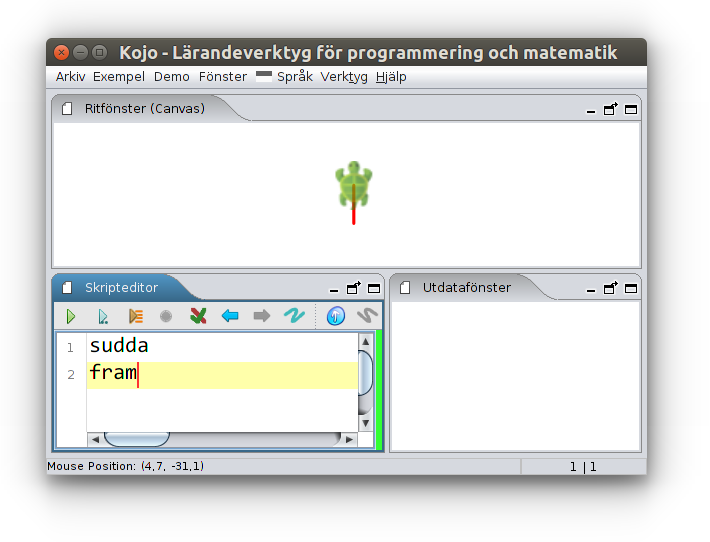
\includegraphics[width=0.8\textwidth]{../img/kojo/kojo.png}
\caption{Den nybörjarvänliga utvecklingsmiljön Kojo för Scala på svenska.}
\label{fig:appendix:ide:kojo}
\end{figure} 

\subsection{Installera Kojo}

Kojo är förinstallerat på LTH:s datorer och körs igång med kommandot \texttt{kojo}. För instruktioner om hur du installerar Kojo på din egen dator se här:\\
\href{http://www.lth.se/programmera/installera/}{lth.se/programmera/installera}

Kojo kräver att \texttt{java} finns på din dator. Eftersom du behöver tillgång till JDK i kursen, är det lika bra att installera hela JDK direkt (och inte bara JRE, så som beskrivs å länken ovan); se vidare hur du gör detta i avsnitt \ref{appendix:compile:install-jdk}. 
%\href{http://www.kogics.net/kojo-download}{www.kogics.net/kojo-download}


\subsection{Använda Kojo}

När du startar Kojo första gången, välj ''Svenska'' i språkmenyn och starta om Kojo. Därefter fungerar grafikfunktionerna på svenska enligt tabell \ref{table:kojo:functions}. När du startat om Kojo inställt på Svenska ser programmet ut ungeför som i figur \ref{fig:appendix:ide:kojo} på sidan \pageref{fig:appendix:ide:kojo}.


Det finns ett antal användbara kortkommando som du hittar i menyerna i Kojo. Undersök speciellt Ctrl+Alt+Mellanslag som ger autokomplettering baserat på det du börjat skriva.


{\small\renewcommand{\arraystretch}{1.45}
\begin{longtable}{@{}p{0.42\textwidth} p{0.55\textwidth}}

\caption{Några av sköldpaddans funktioner. Se även \href{http://lth.se/programmera}{lth.se/programmera}}\label{table:kojo:functions}\\

\emph{Svenska/Engelska} & \emph{Vad händer?}  \\ \hline
%!TEX encoding = UTF-8 Unicode
%!TEX root = ../compendium2.tex

\chapter{Kojo}\label{appendix:kojo}

\section{Vad är Kojo?}

Kojo%
\footnote{\href{https://en.wikipedia.org/wiki/Kojo_(programming_language)}{en.wikipedia.org/wiki/Kojo\_(programming\_language)}}
 är en integrerad utvecklingsmiljö för Scala som är speciellt anpassad för programmeringsundervisning i grundskolan. Kojo används i LTH:s Science Center Vattenhallen för utbildning av grundskolelärare i programmering och vid skolbesök och annan besöksverksamhet, i vilken lärare och studenter vid LTH arbetar som handledare. 
 
 Kojo är öppen källkod och utvecklingsgemenskapen leds av Lalit Pant från Indien. I Kojo finns även lättillgängliga bibliotek som gör tröskeln lägre att programmera rörlig grafik och enkla spel.

Under kursens första laboration använder vi grafikbiblioteket i Kojo för att illustrera grundläggande begrepp, så som sekvens, alternativ, repetition och abstraktion.  


\begin{figure}[H]
\centering
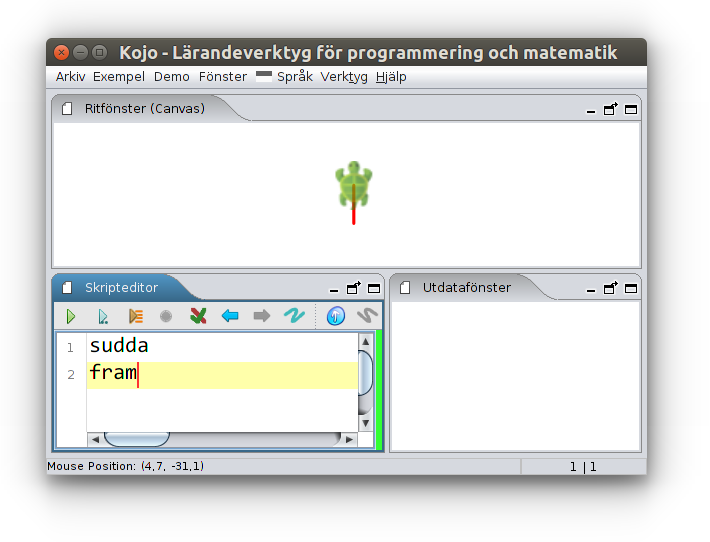
\includegraphics[width=0.8\textwidth]{../img/kojo/kojo.png}
\caption{Den nybörjarvänliga utvecklingsmiljön Kojo för Scala på svenska.}
\label{fig:appendix:ide:kojo}
\end{figure}

\section{Använda grafikbiblioteket i Kojo}\label{appendix:ide:kojo:install}

Kojo bygger på den beprövade pedagogiska idén med sköldpaddsgrafik \Eng{turtle graphics}\footnote{\url{https://en.wikipedia.org/wiki/Turtle_graphics}}, där du skriver program som styr en sköldpadda med en penna under magen. När sköldpaddan rör sig bildas ett streck av valfri färg på skärmen. Beroende på hur du bestämmer att sköldpaddan ska röra sig och vilken färg du bestämmer att pennan ska ha, kan du skapa olika intressanta bilder och samtidigt lära dig om programmeringens grunder.

Under kursens första laboration ska du använda grafikbiblioteket i Kojo tillsammans med editorn VS \code{code} och \code{scala-cli} i terminalen (se appendix \ref{appendix:terminal} och \ref{appendix:compile}). Ladda ner filen \texttt{kojo.scala} från \url{https://cs.lth.se/pgk/kojolib} och spara i en ny katalog med hjälp av din webbläsare, eller via dessa kommandon:

\begin{REPLnonum}
> mkdir w01-kojo
> cd w01-kojo
> curl -o kojolib.scala -sL https://cs.lth.se/pgk/kojolib
\end{REPLnonum}

Nu kan du starta Scala REPL och rita med Kojo så här:

\begin{REPLnonum}
> scala-cli repl .
Welcome to Scala 3.1.2 (17.0.2, Java OpenJDK 64-Bit Server VM).
Type in expressions for evaluation. Or try :help.
                                                                                                                               
scala> fram; höger; fram; vänster

\end{REPLnonum}

Du kan starta VS \code{code} i aktuellt bibliotek så här:
\begin{REPLnonum}
> code .
\end{REPLnonum}

Skriv nedan progam i VS \code{code} och spara det i samma katalog som den tidigare nedladdade filen, under ett nytt valfritt filnamn, t.ex. \code{rita.scala}:

\begin{Code}
@main def rita =
  fram; höger
  fram; vänster
\end{Code}

Kör ditt fristående program med:
\begin{REPLnonum}
> scala-cli run .
\end{REPLnonum}

Du ska nu få upp ett fönster som heter Kojo Canvas med en sköldpadda som ritat två streck. När du stänger fönstret så avslutas programmet. Prova fler sköldpaddsfunktioner enligt tabell \ref{table:kojo:functions}.

I stället för att ladda ned filen \code{kojolib.scala} så kan du placera dess innehåll på lämpligt ställe i ditt program enligt nedan. Observera att raden som börjar med \code{//> using lib} ska vara en enda lång rad utan radbrytningar. Raden med \code{export} gör Kojos kommandon tillgängliga utan prefix:
\begin{CodeSmall}[breaklines=true]
//> using scala "3"
//> using lib "net.kogics:kojo-lib:0.1.1,url=https://github.com/lunduniversity/introprog/releases/download/kojo-lib-0.1.1/kojo-lib-0.1.1.jar"

export net.kogics.kojo.Swedish.*, padda.*, CanvasAPI.*, TurtleAPI.*
\end{CodeSmall}


\noindent Scala-koden för den svenska paddans api finns här: \\
%\href{https://github.com/litan/kojo/blob/master/src/main/scala/net/kogics/kojo/lite/i18n/svInit.scala}{github.com/litan/kojo/blob/master/src/main/scala/net/kogics/kojo/lite/i18n/svInit.scala} \\
\href{https://github.com/litan/kojo-lib/blob/main/src/main/scala/net/kogics/kojo/i18n/Swedish.scala}{github.com/litan/kojo-lib/blob/main/src/main/scala/net/kogics/kojo/i18n/Swedish.scala}


%Kojo kräver (numera) \emph{inte} att \texttt{java} finns på din dator utan kommer med en egen JVM. 
%Eftersom du behöver tillgång till JDK i kursen, är det lika bra att installera hela JDK direkt (och inte bara JRE, så som beskrivs å länken ovan); se vidare hur du gör detta i avsnitt \ref{appendix:compile:install-jdk}.
%\href{http://www.kogics.net/kojo-download}{www.kogics.net/kojo-download}


{\small\renewcommand{\arraystretch}{1.4}
\begin{longtable}{@{}p{0.42\textwidth} p{0.55\textwidth}}

\caption{Ett urval av funktioner i Kojo. Se även \href{http://lth.se/programmera}{lth.se/programmera}}\label{table:kojo:functions}\\

\emph{Svenska/Engelska} & \emph{Vad händer?}  \\ \hline
\code|sudda| \newline \code|clear| & Ritfönstret suddas \\
\code|fram| \newline \code|forward()| & Paddan går framåt 25 steg. \\
\code|fram(100)| \newline \code|forward(100)| & Paddan går framåt 100 steg. \\
\code|höger| \newline \code|right(90)| & Paddan vrider sig 90 grader åt höger. \\
\code|höger(45)| \newline \code|right(45)| & Paddan vrider sig 45 grader åt höger. \\
\code|vänster| \newline \code|left(90)| & Paddan vrider sig 90 grader åt vänster. \\
\code|vänster(45)| \newline \code|left(45)| & Paddan vrider sig 45 grader åt vänster. \\
\code|hoppa| \newline \code|hop| & Paddan hoppar 25 steg utan att rita. \\
\code|hoppa(100)| \newline \code|hop(100)| & Paddan hoppar 100 steg utan att rita. \\
\code|hoppaTill(100, 200)| \newline \code|jumpTo(100, 200)| & Paddan hoppar till läget (100, 200) utan att rita. \\
\code|gåTill(100, 200)| \newline \code|moveTo(100, 200)| & Paddan vrider sig och går till läget (100, 200). \\
\code|hem| \newline \code|home| & Paddan går tillbaka till utgångsläget (0, 0). \\
\code|öster| \newline \code|setHeading(0)| & Paddan vrider sig så att nosen pekar åt höger. \\
\code|väster| \newline \code|setHeading(180)| & Paddan vrider sig så att nosen pekar åt vänster. \\
\code|norr| \newline \code|setHeading(90)| & Paddan vrider sig så att nosen pekar uppåt. \\
\code|söder| \newline \code|setHeading(-90)  | & Paddan vrider sig så att nosen pekar neråt. \\
\code|mot(100,200)| \newline \code|towards(100, 200)| & Paddan vrider sig så att nosen pekar mot läget (100, 200) \\
\code|sättVinkel(90)| \newline \code|setHeading(90)| & Paddan vrider nosen till vinkeln 90 grader. \\
\code|vinkel| \newline \code|heading| & Ger vinkelvärdet dit paddans nos pekar. \\
\code|sakta(5000)| \newline \code|setAnimationDelay(5000) | & Gör så att paddan ritar jättesakta. \\
\code|suddaUtdata| \newline \code|clearOutput| & Utdatafönstret suddas. \\
\code|utdata("hej")| \newline \code|println("hej")| & Skriver texten \texttt{hej} i utdatafönstret. \\
\code|val t = indata("Skriv")| \newline \code|val t = readln("Skriv:")| & Väntar på inmatning efter ledtexten \texttt{Skriv} och sparar den inmatade texten i t.  \\
\code|textstorlek(100)| \newline \code|setPenFontSize(100)| & Paddan skriver med jättestor text nästa gång du gör skriv. \\
\code|båge(100, 90)| \newline \code|arc(100, 90)| & Paddan ritar en båge med radie 100 och vinkel 90. \\
\code|cirkel(100)| \newline \code|circle(radie)| & Paddan ritar en cirkel med radie 100. \\
\code|synlig| \newline \code|visible| & Paddan blir synlig. \\
\code|osynlig| \newline \code|invisible| & Paddan blir osynlig. \\
\code|läge.x| \newline \code|position.x| & Ger paddans x-läge \\
\code|läge.y| \newline \code|position.y| & Ger paddans y-läge \\
\code|pennaNer| \newline \code|penDown| & Sätter ner paddans penna så att den ritar när den går. \\
\code|pennaUpp| \newline \code|penUp| & Lyfter upp paddans penna så att den INTE ritar när den går. \\
\code|pennanÄrNere| \newline \code|penIsDown| & Kollar om pennan är nere eller inte. \\
\code|färg(rosa)| \newline \code|setPenColor(pink)| & Sätter pennans färg till rosa. \\
\code|fyll(lila)| \newline \code|setFillColor(purple)| & Sätter ifyllnadsfärgen till lila. \\
\code|fyll(genomskinlig)| \newline \code|setFillColor(noColor)| & Gör så att paddan inte fyller i något när den ritar. \\
\code|bredd(20)| \newline \code|setPenThickness(20)| & Gör så att pennan får bredden 20. \\
\code|sparaStil| \newline \code|saveStyle| & Sparar pennans färg, bredd och fyllfärg. \\
\code|laddaStil| \newline \code|restoreStyle| & Laddar tidigare sparad färg, bredd och fyllfärg. \\
\code|sparaLägeRiktning| \newline \code|savePosHe| & Sparar pennans läge och riktning \\
\code|laddaLägeRiktning| \newline \code|restorePosHe| & Laddar tidigare sparad riktning och läge \\
\code|siktePå| \newline \code|beamsOn| & Sätter på siktet. \\
\code|sikteAv| \newline \code|beamsOff| & Stänger av siktet. \\
\code|bakgrund(svart)| \newline \code|setBackground(black)| & Bakgrundsfärgen blir svart. \\
\code|bakgrund2(grön,gul)| \newline \code|setBackgroundV(green, yellow)| & Bakgrund med övergång från grönt till gult. \\
\code|upprepa(4){fram; höger}| \newline \code|repeat(4){forward; right}| & Paddan går fram och svänger höger 4 gånger. \\
\code|avrunda(3.99)| & Avrundar 3.99 till 4.0 \\
\code|slumptal(100)| & Ger ett slumptal mellan 0 och 99. \\
\code|slumptalMedDecimaler(100)| & Ger ett slumptal mellan 0 och 99.99999999 \\
\code|systemtid| & Ger nuvarande systemklocka i sekunder. \\
\code|räknaTill(5000)| & Kollar hur lång tid det tar för din dator att räkna till 5000. \\


\end{longtable}
}%end small


\section{Kojo Desktop}

Kojo finns som fristående skrivbordsapplikation, kallad Kojo Desktop. Kojo Desktop innehåller en egen editor med syntaxfärgning för Scala, men fungerar ännu så länge bara för Scala 2. En av de synligaste skillnaderna mellan Scala 2 och Scala 3 är att klammerparenteser vid flerradiga funktioner är nödvändiga i Scala 2, medan Scala 3 har valfria klammerparenteser. Så om du använder Kojo Desktop behöver du komma ihåg att omgärda sekvenser av rader som hör ihop med \code|{| och \code|}|. 

Kojo Desktop är förinstallerat på LTH:s datorer och körs igång med terminalkommandot \texttt{kojo} eller via applikationsmenyn.  För instruktioner om hur du installerar Kojo Desktop på din egen dator se här: \href{http://www.lth.se/programmera/installera/}{lth.se/programmera/installera}

När du startar Kojo första gången, välj ''Svenska'' i språkmenyn och starta om Kojo. Därefter fungerar grafikfunktionerna på svenska enligt tabell \ref{table:kojo:functions}. När du startat om Kojo inställt på svenska ser programmet ut ungefär som i figur \ref{fig:appendix:ide:kojo} på sidan \pageref{fig:appendix:ide:kojo}.

Det finns ett antal användbara kortkommando som du hittar i menyerna i Kojo Desktop. Undersök speciellt Ctrl+Alt+Mellanslag som ger autokomplettering baserat på det du börjat skriva.

\section{Kojo i Webbläsaren}

En begränsad variant av Kojo finns tillgänglig för programmering direkt i din webbläsare här: \url{http://kojo.lu.se/}

När du trycker på play-knappen så kompileras din kod på en server till Javascript via ScalaJS och därefter körs Javascript-koden i din webbläsare. 
Kojo på webben är också ännu så länge begränsad till Scala 2 och kräver att du omgärdar sekvenser av rader som hör ihop med \code|{| och \code|}|.


\section{Mer om Kojo}

I detta dokument finns en enkel introduktion till Kojo: \\ ''Introduction to Kojo'' \url{http://www.kogics.net/kojo-ebooks#intro}


\hline
\end{longtable}
}%end small

\noindent Scala-koden för den svenska paddans api finns här: \\
\href{https://bitbucket.org/lalit_pant/kojo/src/tip/src/main/scala/net/kogics/kojo/lite/i18n/svInit.scala}{bitbucket.org/lalit\_pant/kojo/src/tip/src/main/scala/net/kogics/\\kojo/lite/i18n/svInit.scala}




\newpage

\section{Eclipse och ScalaIDE}\label{appendix:ide:eclipse}

Eclipse%
\footnote{\href{https://en.wikipedia.org/wiki/Eclipse_(software)}{en.wikipedia.org/wiki/Eclipse\_(software)}}
är en professionell IDE som stödjer många olika programmeringsspråk. Eclipse är skriven i Java och bygger vidare på ett utvecklingsprojekt som initierades av IBM. Eclipse är ett fritt och öppet projekt som numera kontrolleras av en oberoende stiftelse.

Till Eclipse finns en insticksmodul \Eng{plug-in} som kallas ScalaIDE och erbjuder stöd för Scala med tillhörande standardbibliotek.

Eclipse är en omfattande och avancerad programmeringsmiljö med många funktioner och inställningar. Det finns även en omfattande uppsättning insticksmoduler och tilläggsprogram som underlättar utveckling av t.ex. webbprogram, databaser och mycket annat. 

I detta avsnitt ges länkar till installation samt tips om hur du kommer igång med att använda Eclipse och ScalaIDE. Det går ganska snabbt att lära sig grunderna, men det kräven en viss ansträngning att lära sig de mer avancerade funktionerna. Det finns omfattande resurser på nätet som hjälper dig vidare. 


\subsection{Installera Eclipse Mars och ScalaIDE}\label{appendix:ide:eclipse:install}

Eclipse med ScalaIDE är förinstallerat på LTH:s datorer och startas med kommandot \texttt{scalaide} i ett terminalfönster.

ScalaIDE fungerar med Eclipse-versionerna \textit{Luna} och \textit{Mars} (men i skrivande stund fungerar ScalaIDE ännu \textit{inte} med den allra senaste versionen kallad \textit{Neon}). 

För att installera ScalaIDE på din egen dator, följ nedan instruktioner: 

\begin{enumerate}
\item Kontrollera enligt avsnitt \ref{appendix:compile:check-jdk} att du har \texttt{java} installerat och installera vid behov JDK enligt avsnitt \ref{appendix:compile:install-jdk}.

\item Installera Eclipse version \textbf{Mars}, varianten för \textbf{Java Developers} som återfinns på denna sida: \\ \url{https://www.eclipse.org/downloads/packages/release/Mars/2} \\ som är den \textit{andra} varianten i listan (alltså inte Java EE). Följ dessa steg:
\begin{enumerate}
\item Klicka på den \textbf{64-bit}-variant som passar ditt operativsystem.
\item Filen som laddas ner heter något som liknar (beroende på OS): \\ \texttt{eclipse-java-mars-2-win32-x86\_64.zip} 
\\ Det kan ta lång tid att ladda ner filen som är på ca 170MB. Om du klickar på \textit{''select a mirror''} kan du välja en svensk sajt för att ladda ner snabbare. 

\item Dubbelklicka på filen för att packa upp den, vilket kan ta många minuter. Du får, när upppackningen är klar, ett bibliotek med en fungerande Eclipse-installation som du kan placera var du vill. Kör du Windows, lägg den förslagsvis här:\\ 
\code|C:\eclipse\eclipse-java-mars-2-win32-x86_64|

\item för Ubuntu Linux finns kompletterande installationsanvisningar här, som ger dig en ikon i app-menyn m.m.: 
\\ \url{http://askubuntu.com/questions/26632/how-to-install-eclipse}
\end{enumerate}

\item Installera Scala IDE inifrån%
\footnote{Det finns på ScalaIDE-hemsidan möjlighet att ladda ner en Eclipse-variant med färdiginstallerad ScalaIDE-plugin, men då får du i skrivande stund den gamla versionen Eclipse \textit{Luna}, varför du rekommenderas att, enligt instruktionerna här, själv installera ScalaIDE inifrån Eclipse \textit{Mars}, som är den senaste Eclipse-versionen för vilken ScalaIDE fungerar.}
 Eclipse enligt nedan steg:
\begin{enumerate}
\item Starta Eclipse, t.ex. genom att köra igång den exekverbara filen som ligger i underbiblioteket \texttt{eclipse}, i Windows heter den \texttt{eclipse.exe} medan den exekverbara filen i Linux heter \texttt{eclipse} utan filändelse.

\item Välj i frågerutan som dyker upp, någon plats för \textit{workspace} (kvittar vilken just nu, kan ändras senare).

\item Klicka på menyn \textit{Help} $\rightarrow$ \textit{Install new software}.

\item Klicka på \textit{Add}-knappen till höger och skriv: \\ \textit{''ScalaIDE for Scala 2.11''} i \textit{Name}-fältet och ange denna adress i \textit{Location}-fältet: \\
  {\small\mbox{\url{http://download.scala-ide.org/sdk/lithium/e44/scala211/stable/site}}} \\
  och klicka \textit{OK}.
  
\item Du får nu upp en lista med alternativ. Kryssa för alternativet
\\ {\frame{\checkmark}}~~\textit{Scala IDE for Eclipse} \\ och klicka \textit{Next} och sedan \textit{Next} igen och acceptera licensvillkoren och klicka \textit{Finish}.

\item Låt installationen ta sin tid och starta sedan om Eclipse när installationen är färdig. 

\item När Eclipse är igång igen visas en dialog som föreslår att du ska köra \textit{Setup Diagnostics}. Gör detta och välj \textit{Use recommended default settings}. Ändra även i filen \textbf{eclipse.ini} för höja den övre minnesgränsen. Det gör du genom att ändra på den rad i filen som börjar med \texttt{-Xmx}. Hur mycket du ska tillåta som max beror på hur mycket minne du har, men ge minst 1 gigabyte för smidig körning, genom att skriva så här på relevant rad i filen \textbf{eclipse.ini}: \\
\texttt{-Xmx1G } \\


\item Kompletterande information finns här, inklusive en video som visar installationsproceduren och hur man kommer igång med ett ''hello world''-program: \\ \url{http://scala-ide.org/download/current.html}


\end{enumerate}


\end{enumerate}

\noindent I nästa avsnitt beskrivs några rekommenderade anpassningar som du kan göra bland de omfattande inställningsmöjligheterna för Eclipse.

\newpage

\subsection{Anpassa Eclipse och ScalaIDE}\label{subsection:appendix:ide:eclipse:tweaks}

\newcommand\Menu[1]{\textit{#1}}
\newcommand\MenuArrow[1]{\Menu{#1}~$\rightarrow$~}
\newcommand\FramedCheckmark[1]{~\frame{\checkmark}~~\textbf{#1}}
\newcommand\FramedUnchecked[1]{$\Box$~\textbf{#1}}
\newcommand\Button[1]{\fbox{\textbf{#1}}}
\newcommand\EclipsePrefs{\MenuArrow{Window}\MenuArrow{Preferences}}
\newcommand\EclipsePrefsGeneral{\EclipsePrefs\MenuArrow{General}}


Förutom maxminneshöjningen i filen \texttt{eclipse.ini}, som finns i installationskatalogen för Eclipse, till minst \texttt{-Xmx1G } (se föregående avsnitt), är det bra att göra några ytterligare anpassningar av Eclipse och ScalaIDE för att få en snabbare och smidigare utvecklingsmiljö. Du hittar inställningarna i menyn \EclipsePrefs ... uppe till höger i Eclipse-fönstret.



\begin{enumerate}
\item \EclipsePrefsGeneral 
\\ Markera \FramedCheckmark{Show Heap Status} så får du se minnesanvändningen i en liten ruta i nederdelen av fönstret, vilket hjälper dig att upptäcka om minnesbegränsningen i filen \texttt{eclipse.ini} är en flaskhals vid stora projekt och många öppna fönster. Klicka sedan \Button{Apply} längst ner.

\item \label{item:scala-perspective} \EclipsePrefsGeneral\MenuArrow{Editors}\MenuArrow{Perspective}  
\\ Markera \textit{Scala} i listan med perspektiv och klicka på knappen 
 \\ \Button{Make default} till höger och sedan på knappen \Button{Apply} längst ner.

\item \EclipsePrefsGeneral\MenuArrow{Editors}\MenuArrow{TextEditors}
\\ Markera \FramedCheckmark{Insert spaces for tabs} så att du slipper specialtecken som kan tolkas olika av olika editorer. Klicka sedan \Button{Apply} längst ner.

\item \EclipsePrefsGeneral\MenuArrow{Editors}\MenuArrow{TextEditors}
\\ \MenuArrow{Spelling} Avmarkera \FramedUnchecked{Enable spell checking} för att slippa att svenska namn och svenska kommentarer markeras som felstavade. Om du senare jobbar med ett projekt helt på engelska, kan du med fördel markera denna kryssruta igen. Klicka sedan \Button{Apply} längst ner.

\item \EclipsePrefsGeneral\MenuArrow{Editors}\MenuArrow{Webbrowser}
\\ Markera \FramedCheckmark{Use external web browser} för att köra din vanliga webbläsare när du klickar på länkar. Klicka sedan \Button{Apply} längst ner.
  
\item  \EclipsePrefs\MenuArrow{Scala}\MenuArrow{Compile}
\\ I fliken \textbf{Standard} markera dessa kryssrutor för att få extra varningar: \\
\begin{tabular}{l @{}l @{}l}
\textit{deprecation} & \FramedCheckmark{} & varnar vid användning av föråldrad kod som snart utgår \\
\textit{feature}     & \FramedCheckmark{} & påminner om import vid användning av avancerad kod  \\
\textit{unchecked}   & \FramedCheckmark{} & ger tips vid speciella problem med generiska typer \\
\end{tabular}\\
och klicka sedan på knappen \Button{Apply} längst ner.

\item \EclipsePrefs\MenuArrow{Java}\MenuArrow{Compiler}\MenuArrow{Errors/Warnings}
\\ Veckla ut listan \textbf{Potential programming problems} och sätt \textbf{Resource leak} till alternativet \textbf{Ignore}, så slipper du varningar vid användning \jcode{Scanner} i Java. Klicka sedan \Button{Apply} längst ner.

\end{enumerate}

\noindent Ovan anpassningar är rekommenderade men inte nödvändiga och du kan gärna välja att göra andra anpassningar som passar just dig. Skriv då gärna ner vilken inställning du ändrat, så att du hittar tillbaka om du ångrar dig. 

Du hittar tips om fler inställningar för att anpassa ScalaIDE här: \\
\url{http://scala-ide.org/docs/current-user-doc/advancedsetup}



\subsection{Använda Eclipse och ScalaIDE}\label{appendix:ide:eclipse:use}

Ett grundläggande koncept i Eclipse är \textbf{workspace}. Ett workspace utgör ett arbetsområde kopplat till en katalog i ditt filsystem där du kan arbeta med ett eller flera \textbf{projekt}. Ett projekt innehåller i sin tur dina källkodsfiler och klassfiler etc. i en specifik katalogstruktur som Eclipse skapar när du editerar, kompilerar och kör dina projekt. 

\subsubsection{Starta och välja workspace}\label{subsubsection:start:eclipse}

När du startar Eclipse måste du välja vilket workspace du vill använda innan du kommer vidare. När du kör igång Eclipse första gången, klicka OK enligt det förslag som ges. Du kan senare växla workspace genom menyn \MenuArrow{File}\Menu{Switch Workspace}. Om katalogen du anger inte redan finns, kommer den att skapas och initieras med de filer Eclipse behöver.

I figur \ref{fig:appendix:eclipse:welcome} visas välkomstfliken i Eclipse med sina länkar till funktionsöversikt och olika handledningar. Stäng välkomstfliken genom att klicka på flikens kryss eller på ikonen \textit{Workbench}. Då kommer du vidare till den normala arbetsytan i Eclipse. Du kan få tillbaka välkomstfliken igen via menyn \MenuArrow{Help}\Menu{Welcome}. 

\begin{figure}[H]
\centering
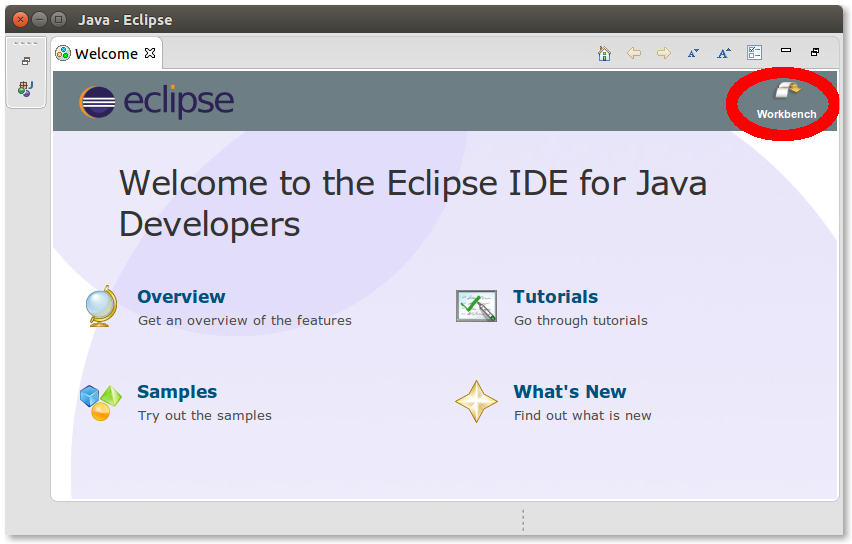
\includegraphics[width=1.0\textwidth]{../img/eclipse/eclipse-welcome.png}
\caption{Välkomstfliken för Eclipse, som nås via menyn \MenuArrow{Help}\Menu{Welcome}. Gå vidare genom att klicka på \textit{Workbench}.}
\label{fig:appendix:eclipse:welcome}
\end{figure}

\subsubsection{Välja perspektiv och visa olika vyer}

Eclipse-fönstret kan innehålla många underfönster i olika flikar, så kallade \textbf{views} eller vyer, som kan arrangeras på olika vis efter hur du vill ha dem. Vilka vyer som syns och hur de placeras beror på vilket s.k. \textbf{perspective} som är aktivt.  Figur \ref{fig:appendix:eclipse:open-perspective} visar arbetsytan med olika vyer i Java-perspektivet. 

Du kan byta till Scala-perspektivet genom att trycka på 
\includegraphics[scale=0.75]{../img/eclipse/eclipse-perspective-button.png} eller genom menyn \MenuArrow{Window}\MenuArrow{Perspective}\MenuArrow{Open Perspective}\MenuArrow{Other...}\Menu{Scala}.
Du kan anpassa inställningarna så att Scala blir \textit{default perspective}, se steg \ref{item:scala-perspective} i avsnitt \ref{subsection:appendix:ide:eclipse:tweaks} på sidan \pageref{subsection:appendix:ide:eclipse:tweaks}.

Stäng vyerna \textit{Task List} och \textit{Outline} om du vill ha mer plats till de övriga vyerna för paketnavigering, editering och utdata. Du kan öppna stängda vyer igen genom menyn \MenuArrow{Window}\Menu{Show View}. 

\begin{figure}
\centering
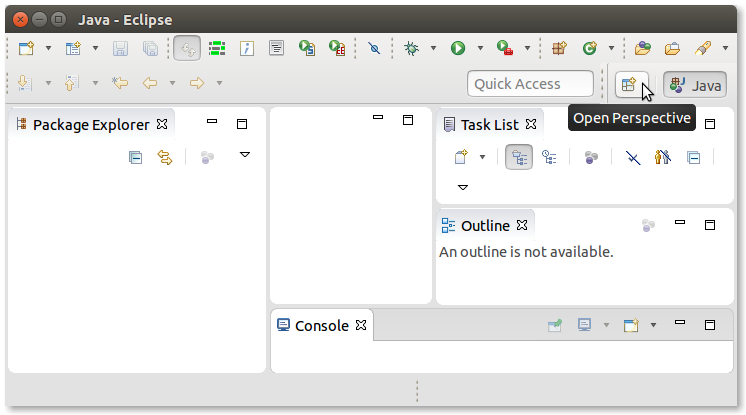
\includegraphics[width=1.0\textwidth]{../img/eclipse/eclipse-open-perspective.png}
\caption{Arbetsytan i Eclipse. Du kan växla mellan Scala- och Java-perspektivet genom att klicka på perspektivvalsknappen.}
\label{fig:appendix:eclipse:open-perspective}
\end{figure}

\subsubsection{Hello World}\label{subsubsection:eclipse:hello-world}

Efter att du öppnat Eclipse med ScalaIDE i ett tomt workspace och valt Scala-perspektivet enligt föregående avsnitt, kan du skapa ditt första projekt med ett \textit{''Hello World''}-program enligt stegen nedan.

\begin{enumerate}
\item Högerklicka i \Menu{Package Explorer} och välj \MenuArrow{New}\Menu{Scala Project}, varefter en dialogruta visas. 

\item Fyll i namnet \texttt{hello} i fältet \Menu{Project Name} och klicka \Button{Finish}.

\item Högerklicka igen i \Menu{Package Explorer} och välj \MenuArrow{New}\Menu{Scala Object}, varefter en ny dialogruta visas. 

\item Fyll i namnet \texttt{hi} i fältet \Menu{Project Name} och klicka \Button{Finish}.

\item Du får nu i editorvyn ett kodskellet med \code{object hi}.

\item Börja skriv \code{main} som visas i figur \ref{fig:appendix:eclipse:complete-main} och tryck Ctrl+Mellanslag för att aktivera kodkomplettering \Eng{code completion}. Då får du upp en lista med alternativ. Välj det översta alternativet \texttt{main} varefter ett kodskellet med en main-metod klistras in automatiskt i din kod.

\begin{figure}
\centering
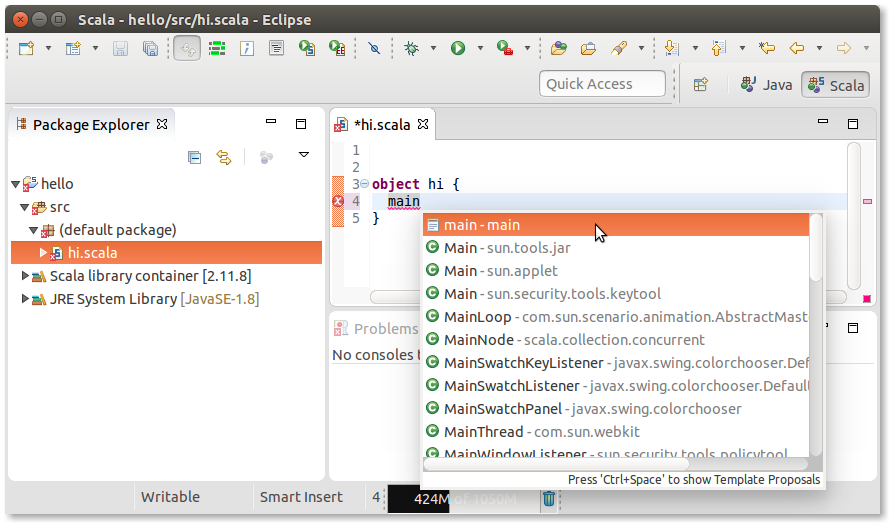
\includegraphics[width=1.0\textwidth]{../img/eclipse/eclipse-complete-main.png}
\caption{Aktivera kodkomplettering med Ctrl+Mellanslag efter ordet \code{main}.}
\label{fig:appendix:eclipse:complete-main}
\end{figure}

\item Fyll i lämplig utskriftstext i ett \code{println}-anrop så att din \code{main}-metod blir så som visas i editorfliken i figur \ref{fig:appendix:eclipse:hello-world}.

\begin{figure}[H]
\centering
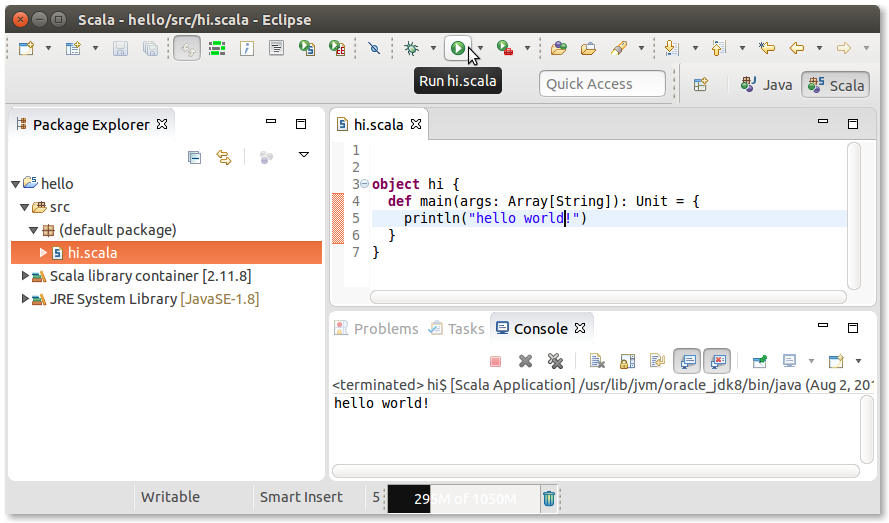
\includegraphics[width=1.0\textwidth]{../img/eclipse/eclipse-hello-world.png}
\caption{Skriv klart \code{main}-metoden och kör ditt program med play-knappen.}
\label{fig:appendix:eclipse:hello-world}
\end{figure}

\item Kör ditt program genom att trycka på den gröna play-knappen, som muspekaren i figur \ref{fig:appendix:eclipse:hello-world} pekar på. Du kan också trycka F11 för att köra igång din app, efter att du vid första körningen i dialogen \textit{Select Preferred Launcher} markerat  \FramedCheckmark{Use configuration specific settings} och valt alternativet \textit{Scala Application (new debugger) Launcher}. 

\end{enumerate}




\subsubsection{Ladda ner kursens workspace och importera projekt till labbarna}

Det finns en zip-fil med ett workspace med projekt för flera av kursens laborationer som du kan ladda ner och importera i Eclipse. Följ stegen nedan.

\begin{enumerate}
\item Ladda ner kursens workspace här: \url{http://cs.lth.se/pgk/ws}

\item Packa upp filen på lämpligt ställe.

\item Starta Eclipse med ScalaIDE-plugin (se startinstruktioner på sidan \pageref{subsubsection:start:eclipse}). 

\item Växla workspace till biblioteket du nyss packade upp, ungefär som i figur \ref{fig:eclipse:ide:open} och klicka \Button{OK}.
\begin{figure}[H]
\centering
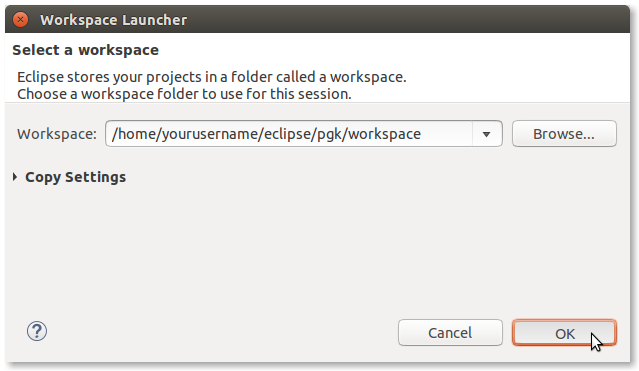
\includegraphics[width=1.0\textwidth]{../img/eclipse/eclipse-select-workspace.png}
\caption {Öppna kursens workspace genom att bläddra till biblioteket där du packade upp filen som du laddat ned från: \url{http://cs.lth.se/pgk/ws} }
\label{fig:eclipse:ide:open}
\end{figure}

\item Stäng välkomstfliken för att komma vidare till workbench (se figur \ref{fig:appendix:eclipse:welcome} på sidan \pageref{fig:appendix:eclipse:welcome}). Det ser då ut ungefär som i figur~\ref{fig:appendix:eclipse:open-perspective} på sidan \pageref{fig:appendix:eclipse:open-perspective}. Det syns ännu inget i \textit{Package Explorer} då vi ännu inte importerat något projekt. 

\item Innan du går vidare, säkerställ att du har Scala-perspektivet aktiverast. Du kan växla till Scala-perspektivet genom att trycka på 
\includegraphics[scale=0.75]{../img/eclipse/eclipse-perspective-button.png} eller genom menyn \MenuArrow{Window}\MenuArrow{Perspective}\MenuArrow{Open Perspective}\MenuArrow{Other...}\Menu{Scala}.
Du kan anpassa inställningarna så att Scala blir \textit{default perspective}, se steg \ref{item:scala-perspective} i avsnitt \ref{subsection:appendix:ide:eclipse:tweaks} på sidan \pageref{subsection:appendix:ide:eclipse:tweaks}.


\item Högerklicka i \textit{Package Explorer} och välj \Menu{Import...}, se Fig.~\ref{fig:eclipse:import}, eller välj menyn \MenuArrow{File}\Menu{Import...}. 

\begin{figure}[H]
\centering
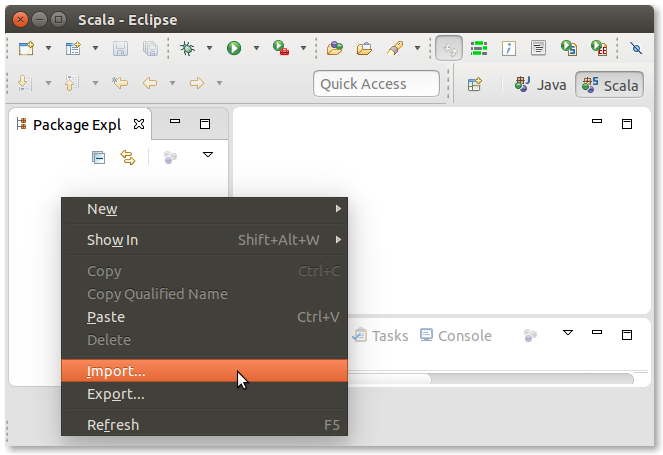
\includegraphics[width=1.0\textwidth]{../img/eclipse/eclipse-import.png} 

\caption {Välj \Menu{Import}-menyn för att importera existerande projekt.}
\label{fig:eclipse:import}
\end{figure}

\item Nu öppnas \Menu{Import}-dialogen som visas i figur \ref{fig:eclipse:import-existing}. Öppna mappen \Menu{General}, markera \textbf{Existing Projects into Workspace} och klicka \Button{Next}.



\begin{figure}[H]
\centering
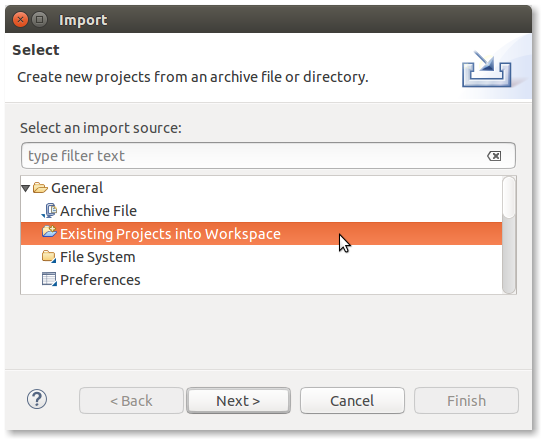
\includegraphics[width=0.75\textwidth]{../img/eclipse/eclipse-import-existing.png} 

\caption {Välj att importera existerande projekt under \Menu{General}.}
\label{fig:eclipse:import-existing}
\end{figure}


\begin{figure}[H]
\centering
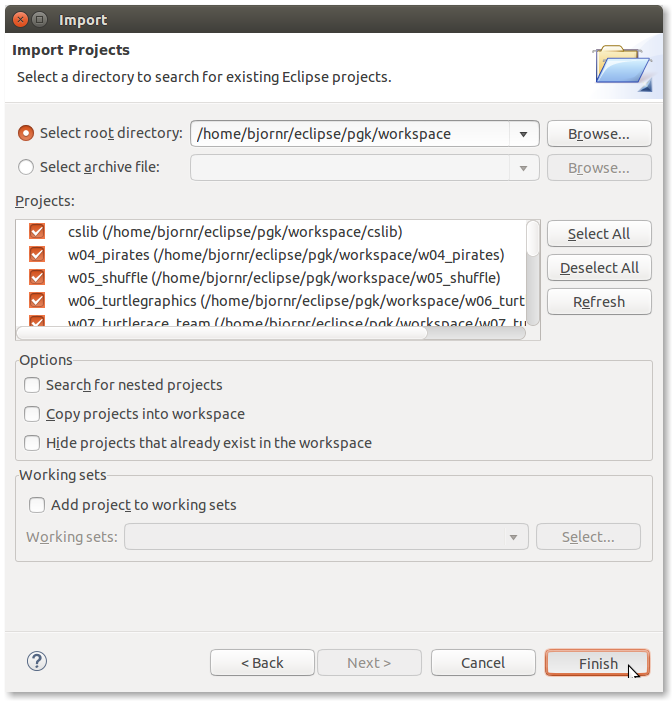
\includegraphics[width=1.0\textwidth]{../img/eclipse/eclipse-import-projects.png} 

\caption {Välj \FramedCheckmark{Select Root Directory} och klicka \Button{Browse}.}
\label{fig:eclipse:import-projects}
\end{figure}


\item Nu kommer ytterligare ett dialogfönster som visas i figure \ref{fig:eclipse:import-projects}. Med \FramedCheckmark{Select Root Directory} markerad kan du klicka \Button{Browse} för att ange workspace-mappen i ännu en dialog där du bara ska trycka \Button{Ok} utan att välja underbibliotek till workspace. När det är klart ska det se ut som i figur \ref{fig:eclipse:import-projects} där alla Eclipse-projekt \FramedCheckmark{cslib}, \FramedCheckmark{w04\_pirates}, etc. är markerade. Klicka sedan \Button{Finish}.

\item Följ ''Hello World''-instruktionerna på sidan \pageref{subsubsection:eclipse:hello-world} och skapa programmet som visas i figure \ref{fig:eclipse:pirates-hi}, genom att veckla ut projektet \textbf{w04\_pirates}, markera och högerklicka på paketet \textbf{priates}, och välja \MenuArrow{New}\Menu{Scala Object}.

\begin{figure}[H]
\centering
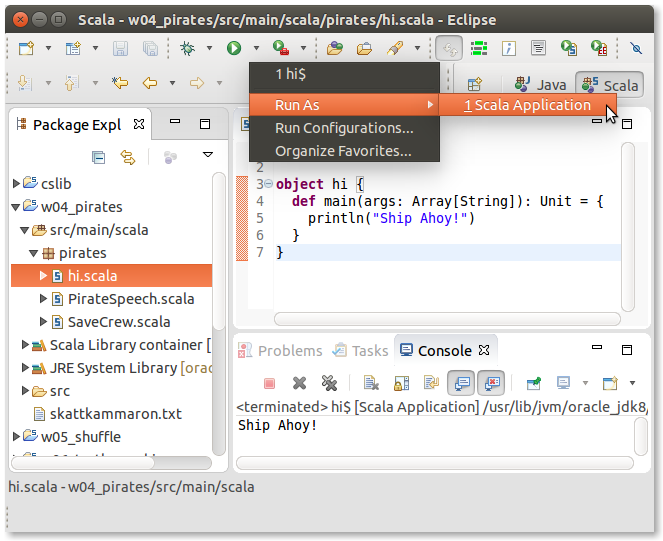
\includegraphics[width=1.0\textwidth]{../img/eclipse/eclipse-pirates-hi.png} 

\caption {Skapa ett \MenuArrow{New}\Menu{Scala Object} med kod enligt bilden.}
\label{fig:eclipse:pirates-hi}
\end{figure}


\end{enumerate}



\newpage

\section{IntelliJ IDEA}\label{appendix:ide:intellij}

IntelliJ IDEA%
\footnote{\href{https://en.wikipedia.org/wiki/IntelliJ_IDEA}{en.wikipedia.org/wiki/IntelliJ\_IDEA}}
 är en professionell IDE som stödjer många olika programmeringsspråk. IntelliJ är skriven i Java och utvecklas av det tjeckiska företaget JetBrains. 

IntelliJ IDEA finns i två varianter: en gratis gemenskapsvariant med öppenkällkodslicens \Eng{Community edition}, samt en betalvariant med stängd källkod och support-tjänster.


Till IntelliJ IDEA finns en insticksmodul \Eng{plug-in} som erbjuder stöd för Scala med tillhörande standardbibliotek..

IntelliJ IDEA är en omfattande och avancerad programmeringsmiljö med många funktioner och inställningar. Det finns även en omfattande uppsättning insticksmoduler och tilläggsprogram som underlättar utveckling av t.ex. webbprogram, databaser och mycket annat. 

I detta avsnitt ges länkar till installation samt tips om hur du kommer igång med att använda IntelliJ IDEA med Scala. Det går ganska snabbt att lära sig grunderna, men det kräven en viss ansträngning att lära sig de mer avancerade funktionerna. Det finns omfattande resurser på nätet som hjälper dig vidare. 

Google tillkännagav 2013 att företaget övergår från Eclipse till IntelliJ som den officiellt understödda utvecklingsmiljön för Android och 2014 lanserades utvecklingsmiljön AndroidStudio%
\footnote {\href{https://en.wikipedia.org/wiki/Android_Studio}{en.wikipedia.org/wiki/Android\_Studio}}
 som bygger vidare på IntelliJ. 

\subsection{Installera IntelliJ med Scala}\label{appendix:ide:intellij:install}

IntelliJ med Scala-plug-in är förinstallerat på LTH:s datorer och startas med kommandot \texttt{intellij} i ett terminalfönster.

\TODO Beskriv hur man installerar IntelliJ med Scala

\subsection{Använda IntelliJ}\label{appendix:ide:intellij:use}

\TODO 

%%!TEX encoding = UTF-8 Unicode
%!TEX root = ../compendium1.tex

\chapter{Fixa buggar}\label{appendix:debug}

\begin{figure}[H]
\centering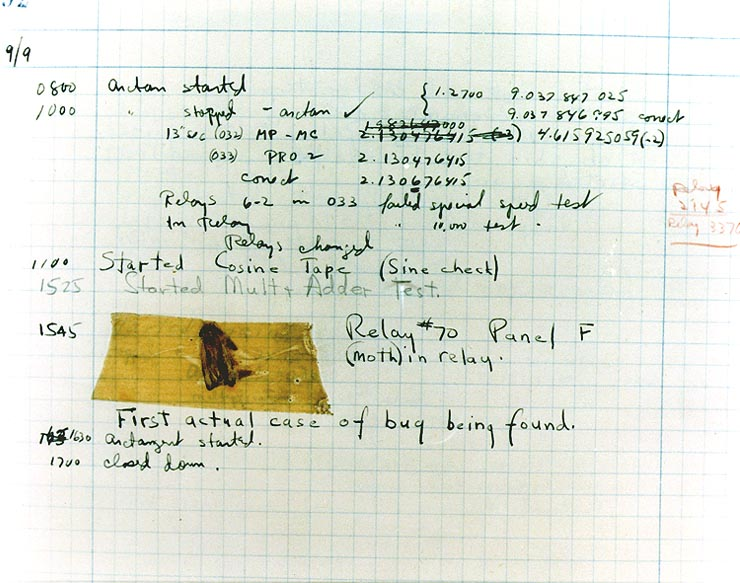
\includegraphics[width=0.85\textwidth]{../img/bug}

\caption{Den första dokumenterade buggen hittades 9 september 1947 i en Mark II Aiken Relay Calculator av Grace Hopper.\protect\footnotemark}

\end{figure}\footnotetext{\href{https://commons.wikimedia.org/w/index.php?curid=165211}{commons.wikimedia.org/w/index.php?curid=165211} Courtesy of the Naval Surface Warfare Center, Dahlgren, VA., 1988. - U.S. Naval Historical Center Online Library Photograph NH 96566-KN, Public Domain.   }


\section{Vad är en bugg?}

En bugg, även kallad lus \Eng{bug}, är en felaktighet som kan göra så att ett program inte beter sig som det är tänkt, och kan innebära oönskad utdata, att programmet kraschar, eller till och med ond bråd död.\footnote{\href{https://www.theguardian.com/technology/2016/jul/01/tesla-driver-killed-autopilot-self-driving-car-harry-potter}{www.theguardian.com/technology/2016/jul/01/tesla-driver-killed-autopilot-self-driving-car-harry-potter}}

Ursprunget till ordets användning i programmeringssammanhang är något oklar, men kan härledas till engelskans \emph{bug} som betyder insekt eller småkryp. 
Man brukar berätta att vid en felsökning av ett program som körde i en tidig dator byggd med  elektromekaniska reläer, uppdagades en död nattfjäril ihjälklämd mellan drivankaret och spolen i ett relä, som orsakade att programmet inte kunde exekveras korrekt. 



\subsection{Olika sorters fel}

När man ska lära sig mer om fel i programvarubaserade system, och hur de kan åtgärdas, är det viktigt att noga skilja på \textbf{misstag} \Eng{mistake}, \textbf{felorsak} \Eng{fault} och \textbf{felyttring} \Eng{failure}. 
Med ''misstag'' menar vi här ett fel som begås av människor (utvecklare, systemadministratörer, operatörer, användare, etc.) medan de skapar och använder ett programvarusystem. 

Det kan bli fel i olika delar av processen: 
\begin{itemize}
\item \textbf{Kravfel} uppstår medan man tänker ut vad systemet ska göra och då misstar sig angående  användarnas behov och önskemål.
\item \textbf{Designfel} uppkommer när man utformar systemets struktur på ett dåligt sätt.
\item \textbf{Implementeringsfel} begås när man programmerar och skriver felaktiga kodrader. 
\item \textbf{Testfel} förekommer vid provkörning av systemet då testkoden är felaktig och därför ger falskt alarm om ''fel'', trots att beteendet egentligen är korrekt.  
\item \textbf{Operatörsfel} sker när systemet lämnas över till de, som ska installera och köra systemet i skarp produktion, och där systemdriften \Eng{operations, ''ops''} sköts på ett sätt som får problematiska konsekvenser.
\item \textbf{Användarfel} händer då användarna ger felaktig indata, eventuellt i strid med riktlinjerna för hur systemet ska användas, som systemet inte klarar att hantera korrekt, varpå mer eller mindre allvarliga felbeteenden hos systemet följer.
\end{itemize} 
I olika delar av utvecklingsprocessen kan alltså misstag begås som, antingen omedelbart, eller någon gång i framtiden, kan orsaka fel. Men det är inte säkert att ett fel någonsin kommer att märkas. Kanske kommer de felaktiga kodraderna, som \emph{skulle} kunna orsaka ett fel, aldrig att exekveras. Eller så kommer ingen användare att någonsin vilja använda systemet så som stipuleras av (onödiga) krav. Det är alltså först när fel \emph{yttrar} sig vid exekvering som misstag märks.

Fel kan också kategoriseras utifrån \emph{hur} de upptäcks i utvecklingsprocessen. Man brukar skilja på fel upptäckta vid granskning, kompileringsfel och exekveringsfel, som diskuteras nedan:
\begin{itemize}
\item Fel upptäckta vid \textbf{granskning}. Ett effektivt sätt att upptäcka fel är att människor noga läser igenom sin egen, och andras kod och försöker leta efter möjliga problem och brister. Man blir ofta ''hemmablind'' när det gäller ens egen kod. Därför kan någon annans, oberoende granskning med ''nya, friska'' ögon vara mycket fruktbar.  I samband med kodgranskning kan man med fördel försöka bedöma  huruvida koden är lätt att läsa, lätt att ändra i eller om koden har andra viktiga kvaliteter som har betydelse för den framtida utvecklingen av koden. Ofta hittar man vid granskning även enkla programmeringsmisstag, så som felaktiga villkor och loop-räknare som inte räknas upp på rätt sätt etc.
  
\item \textbf{Kompileringsfel} uppkommer under kompilering och upptäcks tack vare kontroller som sker av  kompilatorn. 

Vid kompileringsfel får man också ofta av kompilatorn reda på \emph{var} i koden det är fel och \emph{varför} det är fel, så att sökandet efter felorsaken och åtgärdandet av misstaget underlättas. Men ibland är felmeddelandet från kompilatorn missvisande och pekar på helt fel ställe i koden, så det gäller att inte alltid lita blint på det kompilatorn skriver. Dessutom är felmeddelanden från kompilatorn ofta uttryckta i termer av språkets syntaktiska och semantiska regler och det tar tid att lära sig tolka kompilatorers felmeddelanden. Att skapa kompilatorer som ger bra felmeddelande är ett svårt problem som studeras inom den datavetenskapliga disciplinen \textit{kompilatorteknik}, vilken du kan lära mer om i kurser på avancerad nivå.

Olika programmeringsspråk erbjuder olika stora möjligheter att göra kontroller vid kompileringstid. En kompilator för ett språk med ett avancerat typsystem, som till exempel Scala, ger förhållandevis stora möjligheter att identifiera fel redan under kompileringen, medan man med ett språk med ett svagare typsystem, till exempel Javascript, får förlita sig på prestandahämmande kontroller som kompilatorn genererar i maskinkoden eller som du själv väljer att lägga in i källkoden för säkerhets skull. 
  
\item \textbf{Exekveringsfel}, även kallat körtidsfel \Eng{runtime error}, sker medan programmet körs. Det kan krävas viss, specifik indata under specifika exekveringsomständigheter (en viss processor, en viss minnesstorlek, en viss nätverkskapacitet etc.) för att ett exekveringsfel ska yttra sig. När ett exekveringsfel väl yttrar sig, kan olika saker hända:

\begin{itemize}

\item \textbf{Exekveringen ger oönskat resultat.} Det är inte säkert att ett exekveringsfel avbryter exekveringen; det är vanligt att felet ''bara'' resulterar i inkorrekt utdata eller på annat sätt ger dålig kvalitet. För att upptäcka detta innan systemet sätts i drift, är det allmän praxis att man skriver noga uttänkta \textbf{testfall} och analyserar \textbf{testresultat} från exekveringen av  testfallen i detalj genom att undersöka utdata i jämförelse med önskat resultat eller med vad som anses vara en tillräckligt hög kvalitetsnivå.

\item \textbf{Exekveringen hänger sig} \Eng{hang}. Ibland yttrar sig fel genom att inget alls ser ut att hända under exekveringen, vilket kan beror på t.ex.:  
\begin{itemize}[nolistsep]
\item en \textbf{oändlig loop}, som aldrig blir färdig, 
\item att det går \textbf{väldigt långsamt} eftersom bearbetningen av indata tar orimligt lång tid,
\item att programmet \textbf{väntar på indata} som aldrig kommer,
\item att olika jämlöpande delar av programmet väntar på varandra så att ett \textbf{dödläge} \Eng{deadlock} uppstår. 
\end{itemize}

När exekveringen hänger sig och man inte orkar vänta längre på att något ska hända, är det bara att brutalt avbryta exekveringen genom något lämpligt kommando som erbjuds i din körmiljö.\footnote{\texttt{kill -9} $<$pid$>$, Ctrl+C, Ctrl+Shift+C, Ctrl+Z eller något annat beroende på körmiljö.} I värsta fall får man stänga av strömmen.

\item \textbf{Exekveringen kraschar} \Eng{crash}. Ibland blir det ett plötsligt tvärstopp och exekveringen avbryts med ett körtidsfelmeddelande. Detta kan bero på t.ex.:
\begin{itemize}[nolistsep]
\item att \textbf{minnet är slut}, antingen är det parameterminnet för funktionsanrop \Eng{stack memory} som tagit slut eller så är minnet för allokering av objekt som skapas under programmets gång \Eng{heap memory} fullt,
 
\item misstaget att försöka referera en \textbf{null-referens} som inte refererar till något objekt, utan har värdet \code{null}, vilket resulterar i  \textit{null pointer exceeption},

\item att ett s.k. \textbf{undantag} har ''kastats'' \Eng{throw exception} genom att den som skrivit programmet medvetet kodat så att ett oönskat feltillstånd \emph{ska} orsaka en krasch, om inte undantaget ''fångas'' \Eng{catch} och hanteras av omgivande kod. 
\end{itemize}

När systemet kraschar får man en lista med den aktuella kedjan av funktionsanrop i en \textbf{stackspårning} \Eng{stack trace}. Man kan också begära en utskrift av hela innehållet i minnet vid kraschen \Eng{memory dump}, men en sådan kan vara svår att tolka.

\end{itemize}

\end{itemize}

När systemet ger oönskade resultat, hänger sig eller kraschar, får man försöka återskapa exekveringsfelet i en omkörning och, med hjälp av instrumentering eller en debugger, försöka lista ut vad som händer precis \emph{innan} exekveringsfelet uppstår, se  avsnitt \ref{section:debugging}.

I kursen \textit{Programvarutestning} \Eng{Software Testing} lär du dig mer om systematiska metoder för att testa system så att fel kan förebyggas, identifieras och åtgärdas.

\subsubsection{Bugg eller feature?} 

När ett (eventuellt) fel upptäcks, kan det vara på sin plats att först ställa sig några grundläggande  frågor:

\begin{itemize}
\item Är detta verkligen ett ''fel'' eller är det egentligen ett avsett beteende? Det är inte alltid självklart om det är en bugg eller en medvetet skapad systemegenskap/funktion \Eng{feature}.

\item Är det kanske testfallet som har felaktig testkod, medan koden som testas egentligen fungerar alldeles utmärkt? Sådan problem kan vara speciellt svåra att lösa, då man ofta letar på fel ställe efter orsaken.

\item Om buggen rör någon kvalitetsegenskap hos systemet kan man fråga sig: Var går egentligen gränsen för ''fel''? Är detta bra nog givet vad det kostar att förbättra kvaliteten? Kvalitetskrav berör egenskaper hos ett program som kan uttryckas på en glidande skala, där något kan vara mer eller mindre \emph{bra} eller \emph{dåligt} ur olika synvinklar. Sådana krav leder ofta till viktiga men svåra avvägningsbeslut under design och implementation. Dessutom kan testresultat bli svårbedömda och det kan finnas olika åsikter om huruvida ett eventuellt fel är en bugg eller inte.

Här är några exempel på kvalitetskrav:
\begin{itemize}
\item \textbf{Prestandakrav} \Eng{performance requirements} avser hur snabbt och effektivt programmet ska arbeta under olika omständigheter.
 
\item \textbf{Kapacitetskrav} \Eng{capacity requirements} avser hur mycket data systemet ska klara av under olika omständigheter.

\item \textbf{Användbarhetskrav}\footnote{\href{https://sv.wikipedia.org/wiki/Anv\%C3\%A4ndbarhet}{sv.wikipedia.org/wiki/Användbarhet}} \Eng{usability requirements} avser krav på hur lättanvänt systemet ska vara för en given användarkategori. 
\end{itemize} 

\end{itemize}

I kursen \textit{Kravhantering} \Eng{Sofware Requirements Engineering} lär du dig mer om att identifiera, specificera och följa upp kvalitetskrav.

\subsubsection{Felärendehanteringsverktyg} 

Det är allmän praxis i industriell systemutveckling att använda sig av ett felärendehanteringsverktyg \Eng{issue tracker} så att samarbetande utvecklare får stöd i att hålla reda på alla uppkomna fel och problem \Eng{issue}. Många av de populära kodlagringsplatserna som finns på nätet, så som GitLab, GitHub och BitBucket (se avsnitt \ref{section:code-hosting}), erbjuder felärendehanteringsfunktioner. Dessa kan till exempel vara:
\begin{itemize}
\item hantering och sammanställning av alla olika ärendetillstånd, så att man kan se vilka issues som är i tillstånden \textit{Open} eller \textit{Closed},
\item tillording av ärende till specifika personer som ska åtgärda problemet,
\item gradering av ärende i olika allvarlighetsgrader,
\item meddelandegenerering till inblandade personer när ett ärende kommenteras eller ändrar tillstånd.
\end{itemize}


\section{Att förebygga fel}

Även om det nästan är oundvikligt att inte låta buggar slinka in i koden allteftersom den blir mer och mer komplex, är det ändå viktigt att lägga stor möda vid att försöka undvika att så sker. Det är ofta mycket bättre investerad tid att jobba med buggförebyggande åtgärder medan du skapar koden, än att jaga buggar som skulle kunna ha undvikts med allmän noggrannhet och stramare disciplin i kodningen. Nedan sammanfattas några åtgärder som kan hjälpa till att minska mängden fel.

\begin{itemize}
\item \textbf{Skapa begriplig kod}. Grunden för att undvika buggar är anstränga sig att skriva begriplig kod som är lätt att läsa. Detta är en ständig kamp; kodens komplexitet växer för varje tillägg och med jämna mellanrum behövs omstruktureringar \Eng{refactoring} för att bibehålla en god struktur som underlättar begripligheten och gör utvidgningar lättare. 
%En integrerad utvecklingsmijlö erbjuder stöd för att omstrukturera kod  med bibehållen korrekthet. 

\item \textbf{Tänk ut bra namn}. En viktig pusselbit för att skapa begriplig kod är att tänka ut bra namn. Detta kan vara förvånansvärt svårt och kan kräva mycket diskussioner och tankemöda. 
%I själva namnet ligger ofta en stor del av möjligheten för en abstraktion du skapat att nå ut till dina medutvecklare med rätt associationer, som genom sitt namn antingen kan skapa härligt läsbar programtext, eller oerhört svårigenomtränglig gröt där namnen snarast upplevs som desinformation. 
Om du inser att ett namn är illa valt är det förmodligen värt jobbet att omstrukturera koden och införa ett bättre namn, speciellt om andra ännu inte vant sig alltför mycket vid begreppet. 
%Ibland när ett namn ''kliar'' beror det på att själva abstraktionen är feltänkt och behöver tänkas om. 
%En integrerad utvecklingsmiljö erbjuder stöd för att byta namn på precis rätt ställe, med hänsyn till synlighet och blockstruktur. 

\item \textbf{Kontrollera parametrar och variabler}. Ofta vet känner man till vilka villkor som måste gälla för olika variablers värden. Till exempel vet man ofta att en viss funktionsparameter av heltalstyp inte får vara negativ. Då kan man säkerställa detta genom att lägga in kontroller av att villkoret är uppfyllt. Vid villkor som gäller parametrar, brukar man i Scala anropa \code{require}, till exempel: \code{require(x >= 0, "x must be positive")}. Det finns också en metod \code{assert} som fungerar på samma vis\footnote{\href{http://stackoverflow.com/questions/26140757/what-to-choose-between-require-and-assert-in-scala}{stackoverflow.com/questions/26140757/what-to-choose-between-require-and-assert-in-scala}}; medan \code{require} används för att kontrollerar parametrar, brukar \code{assert} användas för att kontrollera generella villkor som ska gälla, till exempel \code{assert(x + y > n, "overflow")}.  Fördelen med att lägga in kontroller av villkor är att villkorsbrott upptäcks direkt och felsökningen blir lättare. 

\item \textbf{Kontrollera typer}. Med \textit{typannoteringar} får du hjälp av kompilatorn att kontrollera dina hypoteser om vilka typer olika värden har. I Scala kan du nästan var du vill i ett uttryck lägga till ett kolon och en typ för att begära att kompilatorn kontrollerar typen. Till exempel kan du skriva \code{(xs + f(42)) : Set[Int]} för att säkerställa att uttrycket \code{xs + f(42)} verkligen ger en mängd med heltal. Även om du sällan i Scala behöver ange typer explicit, tack vare kompilatorns typinferens, bidrar det till läsbarheten och skapar säkrare kod om du på lämpliga ställen ändå anger de typer som du förväntar dig, speciellt vid i komplicerade uttryck eller långa kedjor av metodanrop, och när metoders returtyper inte är uppenbara. Dessutom kan kompilatorn ibland undvika att gå vilse i speciellt svåra typhärledningar, om du hjälper den på traven med explicita typannoteringar.

\item \textbf{Hantera saknade värden}. Det är mycket vanligt att man måste hantera situationer där ett värde saknas, inte kan beräknas, eller inte finns tillgängligt av andra orsaker. Man kan hålla reda på att ett värde saknas genom att representera detta med speciella värden, t.ex. \code{-1} eller \code{null}. Men den strategin leder mycket lätt till buggar, då man lätt glömmer att på andra ställen i koden kontrollera dessa speciella värden. Med sådana speciella värden får man heller ingen hjälp av kompilatorn att upptäcka att man missat att ta hand om dem. Om man istället hanterar eventuellt saknade värden med \code{Option} (se kapitel \ref{chapter:W08}), så får man hjälp vid kompileringstid och slipper exekveringsfel och besvärlig felsökning. Det blir dessutom väldigt tydligt för alla som läser din kod, inklusive du själv, att ett värde kan saknas.
 
\item \textbf{Hantera undantag}. När undantag uppstår, t.ex. att en fil inte kan läsas eller det blir division med noll, avbryts exekveringen och programmets användare kan inte använda programmet längre, vilket i värsta fall kan få ödesdigra konsekvenser. Därför vill man hantera undantagssituationer på ett sådant sätt att programmet blir robust och inte kraschar. Detta kan man med fördel göra genom att kapsla in undantaget i ett värde av typen \code{Try}, se kapitel \ref{chapter:W08}. I likhet med \code{Option} för saknade värden, blir det tydligt i koden att ett värde av typen \code{Try} kan innebära ett lyckat resultat (\code{Success}), eller så fallerar beräkningen (\code{Failure}) med en inkapslad, förhindrad krasch. 

\item \textbf{Granska kod}. Det är allmän praxis i industriell programvaruutveckling att göra kodgranskningar, vid vilka en grupp människor noga studerar någon annans kod och ger kommentarer och identifierar potentiella problem. Ofta har man en checklista att utgå ifrån medan man läser koden, som innehåller punkter man vill kontrollera speciellt, t.ex. begriplighet, namngivning, kontroller av parametrar, hantering av saknade värden och undantag, etc. Många organisationer har en överenskommen kodningsstandard med riktlinjer för kodens utseende och stil som alla ska följa om inte speciella skäl finns. Att sådana stilriktlinjer följs kan kontrolleras genom granskningar. Det finns också verktygsstöd för att göra sådana kontroller. Ett exempel på kodningsriktlinjer för Scala finns på den officiella dokumentationssajten\footnote{\url{http://docs.scala-lang.org/style/scaladoc.html}}. 

\item \textbf{Testa kod}. Det är allmän praxis i industriell programvaruutveckling att genomföra tester på flera olika nivåer. Man kombinerar ofta \textbf{enhetstest} \Eng{unit test} av enskilda delar av koden, med \textbf{funktionstest} \Eng{feature test} för att se så att indata i en tänkt användningssituation ger önskat resultat, och \textbf{systemtest} \Eng{system test} för att se att alla delar fungerar tillsammans under realistiska omständigheter. 

\item \textbf{Lär av användarnas upplevelser}. När koden sätts i produktion finns möjlighet att lära sig genom återkoppling från användare. Hur systemet används och hur användarna upplever det att använda systemet är mycket viktig information när man ska besluta om hu koden bäst ska utveckla vidare. Från användarna kan man få reda på både okända buggar och få briljanta idéer till nya värdefulla funktioner. En mjukvaruutvecklande organisations innovationsförmåga beror i stor utsträckning på dess förmåga att kontinuerligt leverera kod som får allt fler funktioner som användarna gillar, utan att för många irriterande eller ödesdigra buggar.

\end{itemize}



\section{Vad är debugging?}

När en felyttring identifierats, t.ex. genom testning eller slutanvändare rapporterar om problem, vidtar sökandet efter den bakomliggande felorsaken, så att vi förstår \emph{varför} det blev fel och sedan kan \emph{åtgärda} misstaget. Denna process kallas \textbf{avlusning} \Eng{debugging}.




\subsection{Hur hitta felorsaken?}

Första steget i avlusningsprocessen är att hitta den bakomliggande felorsaken. Detta kan vara mycket svårt, speciellt om systemet är stort och komplicerat.

När du stirrar dig blind på koden utan att hitta felorsaken, kan det bero på att du har en felaktig hypotes om vad koden egentligen gör. Du är övertygad om att en viss sak händer, men \emph{egentligen} är det \emph{inte} det du \emph{tror} händer som \emph{verkligen} händer. Exempelvis kanske du antar att en räknare räknas upp i en loop, men i själva verket saknas uppräkningen. Om du oreflekterat accepterar ditt felaktiga antagande, är det stor risk att du letar på fel ställe i koden.

Följande åtgärder är ofta lämpliga när man jagar buggar:


\begin{itemize}

\item \textbf{Återskapa buggen med ett minimalt testfall}. 
När du upptäckt en felyttring är det viktigt att kunna återskapa felet, så att koden som körs precis \emph{innan} buggen uppstår kan felsökas. Allra bäst är det om du kan skapa ett \textbf{minimalt testfall} där precis den minimala indata och de enskilda förutsättningar nedtecknas, som ska gälla för att buggen ska uppstå. Beskrivningen av det minimala testfallet är första pusselbiten i det detektivarbete som vidtar under felsökningen.

\item \textbf{Formulera och verifiera hypoteser om buggen}. En grundläggande princip vid felsökning är att uttryckligen formulera hypoteser som du har om vad som sker i systemet medan buggen uppstår och sedan \emph{verifiera} att de verkligen stämmer, genom olika undersökningar av det exekverande systemet. Du ska alltså tydligt beskriva hur du tror att koden fungerar och sedan med olika former av instrumentering, t.ex. genom utskrifter i terminalen av variablers värden, kontrollera att så verkligen är fallet. Detta kan göras med instrumentering enligt nedan.

\item \textbf{Instrumentering med utskrifter, ''print-debugging''}.

För att verifiera din hypotes om vad som leder fram till buggen, behöver du kontrollera vad som händer. Det kan du göra genom att på väl valda ställen ligga in \code{println}-utskrifter i koden där värden på intressanta variabler skrivs ut. Det kan behövas lite klurighet för att hitta precis rätt utskrifter; om man skriver ut allt som händer i alla loopar drunknar man i all information, men skriver man ut för lite förbiser man kanske den falsifierade hypotesen och får ingen hjälp att knäcka bugg-gåtan.  

Du kan även använda en avlusare \Eng{debugger}, som normalt ingår i en integrerad utvecklingsmiljö, för att instrumentera din kod. Se vidare i avsnitt \ref{section:debugging} om hur du använder avlusarna i Eclipse och IntelliJ IDEA.

\end{itemize}



\section{Åtgärda fel}

Ofta är det det svåraste att \emph{hitta} buggen, medan själva buggrättningen visar sig trivial. Har du, till exempel, väl hittat den saknade uppräkningen av din loop-variabel är det uppenbart vad du ska göra.

Men ibland är det riktigt knepigt att åtgärda felet. Nedan sammanfattas några av de situationer som kan uppkomma, som gör att felrättningen blir extra svår. 

\begin{itemize}
\item Kanske är själva algoritmen i grunden feltänkt och en helt ny algoritm behöver konstrueras. Att skapa nya algoritmer från grunden kan visa sig mycket svårt i en del fall. I fortsättningskurser får du lära dig mer om algoritmkonstruktionens ädla konst.

\item Kanske algoritmen fungerar för olika normalfall, medan ovanliga undantagsfall inte hanteras korrekt. Att på ett bra sätt hantera alla upptänkliga fall kan visa sig väldigt knepigt. Tyvärr är det ofta undantagsfall i kombination med buggar som öppnar för säkerhetsluckor redo att utnyttjas av elaka hackare för att krascha systemet eller smitta ner det med virus.

\item Kanske är problemet i sig väldigt svårt att lösa på ett korrekt sätt. Algoritmen kan vara riktigt knepig med många villkor, loopar och nästlade datastrukturer. Blir det fel i en sådan algoritm kan det ta lång tid att få ändringar att fungera och alla villkor, loopar och nästlade datastrukturer att passa ihop igen efter felrättningen. 

\item Medan man rättar en bug kan man råka att, av misstag, skapa nya buggar. Risken för detta är speciellt stor om koden är komplex. Ibland låter man till och med bli att åtgärda ett fel om systemet ändå fungerar hjälpligt i andra avseenden och risken är för stor att nya buggar skapas. Då behöver systemet strukturerats om så att det blir lättare att ändra i.

\item Kanske växer exekveringstiden exponentiellt med datamängden. Det kan då i praktiken vara omöjligt att skriva ett program som i alla lägen blir färdigt inom rimlig tid. Då får man försöka tänka ut kluriga genvägar till suboptimala lösningar som ändå duger, vilket ibland kräver mycket avancerad programmeringsteknik.
 
\end{itemize}

Det finns ingen allenarådande snabbfix att ta till när man stöter på svåra fel. Att bli en produktiv  systemutvecklare, som framgångsrikt reder ut allehanda buggar, handlar i stor utsträckning om att kombinera en bred allmänbildning inom datavetenskap med ett livslångt lärande, där varje bugg du hittar och åtgärdar ger dig nya kunskaper och erfarenheter inför framtiden.
Även om din bugg är irriterande, försök se den som en ny chans till ökad lärdom!



\section{Använda en debugger}\label{section:debugging}

Med en professionell integrerad utvecklingsmiljö kommer ofta en avancerad debugger, som kan hjälpa dig att följa exekveringen och se vad som händer medan koden kör. Normalt ingår dessa funktioner i en debugger: 

\begin{itemize}
\item \textbf{Sätta brytpunkter}. Med hjälp av debuggern kan du sätta så kallade \textit{brytpunkter} på speciella ställen i koden. Detta görs ofta genom att du markerar en kodrad i marginalen varpå en brytpunktssymbol placeras där. När exekveringen når brytpunkten avbryts exekveringen och du kan stega dig vidare eller inspektera variablers värden vid brytpunkten.  
\item \textbf{Stegad exekvering}. När du nått en brytpunkt kan du med hjälp av debuggern stega dig fram genom koden rad för rad och se vad som händer. Om du kommer till ett funktionsanrop kan du välja att stega in i koden som implementerar funktionen eller bara köra funktionen i ett svep och stega till nästa rad som kommer efter funktionsanropet. Det kan kräva många omkörningar från en viss brytpunkt, innan man hittar vilka funktioner som inte verkar relevanta alls för buggen och bara kan stegas över, eller vilka funktioner som utgör gåtans lösning och som du vill stega in i och undersöka närmare. Stegar man djupt ner i funktionsanropskedjan, går man lätt vilse och får börja om. (Det går inte att stega bakåt...)
 
\item \textbf{Inspektera variabler}. Medan du stegar dig fram i koden kan du inspektera variablers värden. I ett område på skärmen presenterar debuggern både enkla värden så som heltal och strängar, men även datastrukturer, så som vektorer och listor, kan inspekteras genom att debuggern låter dig bläddra bland arrayer och objektreferenser. Ett program kan ha väldigt många variabler och djupa strukturer av objekt som refererar till nya objekt. Det är ofta ett knepigt detektivarbete att försöka lista ut hur olika variabelvärden relaterar till orsaken bakom buggen som du letar efter. Du behöver ofta växla mellan att läsa koden, stega dig fram, sätta nya brytpunkter och inspektera variabler för att förstå vad som händer. 

\end{itemize}

\noindent I Kojo (se appendix \ref{appendix:kojo}) finns enkla debug-funktioner. Man kan till exempel följa stegen i exekveringen med hjälp av den brandgula play-knappen ''Kör och spåra programmet'' (kortkommando: Alt+Enter). Då öppnas ett nytt fönster som visar exekveringsstegen. Man kan klicka på ett steg och få  information om parametrar vid funktionsanrop etc.

Du kan läsa mer om hur man använder en avancerad debugger i en professionell integrerad utvecklingsmiljö i appendix \ref{appendix:ide}.


%%!TEX root = ../compendium.tex

\chapter{Dokumentation}

\section{Vad gör ett dokumentationsverktyg?}

\section{scaladoc}

\section{javadoc}
%%!TEX encoding = UTF-8 Unicode
%!TEX root = ../compendium2.tex

\newcommand{\sbt}{\texttt{sbt}}

\chapter{Byggverktyg}\label{appendix:build}

\section{Vad gör ett byggverktyg?}

Ett \textbf{byggverktyg} \Eng{build tool} används för att
\begin{itemize}
\item ladda ner,
\item kompilera,
\item testköra,
\item paketera och
\item distribuera
\end{itemize}
programvara. Ett stort utvecklingsprojekt kan innehålla många hundra kodfiler och under utvecklingens gång vill man kontinuerligt testköra systemet för att kontrollera att allt fortfarande fungerar; även den kod som inte ändrats, men som kanske ändå påverkas av ändringen. Ett byggverktyg används för att \textit{automatisera} denna process.

Ett viktigt begrepp i byggsammanhang är \textbf{beroende} \Eng{dependency}. Om koden X behöver annan kod Y för att fungera, sägs kod X ha ett beroende till kod Y.

I konfigurationsfiler, som är skrivna i ett format som byggverktyget kan läsa, specificeras de beroenden som finns mellan olika koddelar. Byggverktyget analyserar dessa beroenden och, baserat på ändringstidsmarkeringar för kodfilerna, avgör byggverktyget vilken delmängd av kodfilerna som behöver \textbf{omkompileras} efter en ändring. Detta snabbar upp kompileringen avsevärt jämfört med en total omkompilering från grunden, som för ett stort projekt kan ta många minuter eller till och med timmar. Efter omkompilering av det som ändrats, kan byggverktyget instrueras att köra igenom testprogram och rapportera om testernas utfall, men även ladda upp körbara programpaket till t.ex. en webbserver.


En vanlig typ av beroende är färdiga programbibliotek som utnyttjas av systemet under utveckling, vilket i praktiken ofta innebär att en sökväg till den kompilerade koden för programbiblioteket behöver göras tillgänglig. I JVM-sammanhang innebär detta att sökvägen till alla nödvändiga jar-filer behöver finnas på sökvägslistan kallad \textbf{classpath}.

Många byggverktyg kan utföra så kallad \textbf{beroendeupplösning} \Eng{dependency resolution}, vilket innebär att nätverket av beroenden analyseras och rätt uppsättning programpaket görs tillgänglig under bygget. Detta kan även innebära att programpaket som är tillgängliga via nätet automatiskt laddas ned inför bygget, t.ex. via lagringsplatser för öppen källkod.

Även om man bara har ett litet kodprojekt med några få kodfiler, är det ändå smidigt att använda ett byggverktyg. Man kan nämligen göra så att byggverktyget är aktivt i bakgrunden och, så fort man sparar en ändring av koden, gör omkompilering och rapporterar eventuella kompileringsfel.

Det är klokt att kompilera om ofta, helst vid varje liten ändring, och rätta eventuella fel \textit{innan} nya ändringar görs, eftersom det är mycket lättare att klura ut ett enskilt problem efter en mindre ändring, än att åtgärda en massa svåra följdfel, som beror på en sekvens av omfattande ändringar, där misstaget begicks någon gång långt tidigare.

En integrerad utvecklingsmiljö, så som VS Code eller IntelliJ IDEA, bygger om koden kontinuerligt och kan ofta konfigureras att kommunicera med flera olika byggverktyg. Exempelvis kan du med VS Code välja om du vill att Scala CLI eller \sbt~ ska användas för att bygga ditt projekt.

Det finns många olika byggverktyg. Några allmänt kända byggverktyg listas nedan så att du ska känna igen vilket byggverktyg som används i öppen-källkods-projekt som du stöter på, t.ex. på GitHub.

\begin{itemize}

\item \texttt{Scala CLI}. Verktyget Scala CLI (Command Line Interface) är öppen källkod utvecklad av VirtusLab\footnote{\url{https://scala-cli.virtuslab.org/}} för att kompilera och köra Scala- och Java-program och innehåller också grundläggande byggverktygsfunktioner, så som att köra testfall, paketera jar-filer och skapa dokumentation. Kommandot \code{scala-cli} övertog år 2023 rollen som det officiella \code{scala}-kommandot. Detta är det enklaste och rekommenderade sättet att bygga system med Scala-kod. Grundläggande användning av Scala CLI beskrivs i Appendix \ref{appendix:compile:scala-cli}, medan en mer utförlig beskrivning återfinns nedan i avsnitt \ref{appendix:build:scala-cli}.

\item \sbt. Även kallad \textit{Scala Build Tool}. Används för att bygga Java- och Scala-program i samexistens, men även för att automatisera en mängd andra saker. \sbt~är utvecklat i Scala och konfigurationsfilerna, som heter \texttt{build.sbt}, innehåller Scala-kod som styr byggprocessen. \sbt~är avancerat och klarar bygga system som består av många projekt \Eng{multi-project build}. \sbt~är det i särklass vanligaste byggverktyget för Scala och många öppen-källkodsprojekt använder \sbt. Läs mer om \sbt~i avsnitt \ref{appendix:build:sbt} nedan.

Efter kritik om att \sbt~är komplicerat så har flera alternativa byggverktyg för Scala utvecklats, däribland \code{bleep}\footnote{\url{https://bleep.build/docs/}} och \code{mill}\footnote{\url{https://mill-build.com/mill/Intro_to_Mill.html}}. 


\item Apache Maven, \texttt{mvn} är också skriven i Java och är en efterföljare till \texttt{ant}. Maven används av många Java-utvecklare. Konfigurationsfilerna heter \texttt{pom.xml} och innehåller en s.k. projektobjektmodell specificerad i XML enligt  speciella regler.

\item \texttt{gradle} bygger vidare på idéerna från \texttt{ant} och \texttt{maven} och är skrivet i Java och Groovy.  Konfigurationsfilerna skrivs i Groovy och heter \texttt{build.gradle}.

\item Apache \texttt{ant}. Detta byggverktyg är utvecklat i Java som ett alternativ till \texttt{make} och används fortfarande i många Java-projekt, även om Maven och Gradle är vanligare numera. Konfigurationsfilerna heter \texttt{build.xml} och skrivs i det standardiserade språket XML enligt  speciella regler.

\item \texttt{make}. Detta anrika byggverktyg har varit med ända sedan 1970-talet och används fortfarande för att bygga många system under Linux, och är populärt vid utveckling med programspråken C och C++. En konfigurationsfil för \texttt{make} heter \texttt{Makefile} och har en egen, speciell syntax.
\end{itemize}

\section{Scala Command Line Interface \texttt{scala-cli}}\label{appendix:build:scala-cli}

Utvecklingen av \href{https://scala-cli.virtuslab.org/}{Scala CLI} påbörjades 2022 av \href{https://virtuslab.com/}{Virtuslab}. Scala CLI blev 2023 det officiella byggverktyget för enkla Scala-projekt och medföljer \href{https://www.scala-lang.org/download/}{installationen av Scala}. Scala CLI kan även installeras separat och köras med kommandot \code{scala-cli}, men blir under 2023 liktydigt med kommandot \code{scala} i terminalen.\footnote{I skrivande stund har gamla \code{scala}-kommandot ännu inte uppgraderats, men det förväntas ske innan höstterminen startar. När så väl sker kan alla förekomster av \code{scala-cli} i detta stycke ersättas med det kortare kommandot \code{scala}.}

Efter nyinstallation av Scala CLI kan du ange följande kommando för att, en gång för alla, få tillgång till kompletteringar av optioner med Tab-tangenten i terminalen:
\begin{REPLsmall}
scala-cli install-completions 
\end{REPLsmall}

Innan du börjar skriva källkod i en ny katalog i VS Code kan du konfigurera VS Code att vara redo för att använda Scala CLI som byggverktyg i aktuell katalog med följande kommando (vänta med att öppna VS Code till efter att du kört kommandot): 
\begin{REPLsmall}
mkdir minNyaKatalog
cd minNyaKatalog
scala-cli setup-ide . 
code .
\end{REPLsmall}
	

\subsection{Grundläggande byggfunktioner i Scala CLI}

De grundläggande funktionerna sammanfattas nedan (se även Appendix \ref{appendix:compile:scala-cli}):

\begin{table}[H]
\begin{tabular}{l p{6.5cm}}
\texttt{scala-cli repl} & Starta Scala REPL.  Det går även bra med enbart \texttt{scala-cli}\\
\texttt{scala-cli repl hello.scala} & Starta Scala REPL med kompilerade koden i \texttt{hello.scala} på classpath.  \\
\texttt{scala-cli repl .} & Starta repl med kodfiler i aktuell katalog tillgängliga på classpath. \\
\texttt{scala-cli compile hello.scala} & Kompilera koden i filen \texttt{hello.scala}  \\
\texttt{scala-cli compile .} & Kompilera alla kodfiler i aktuell katalog. \\
\texttt{scala-cli run hello.scala} & Kompilera koden i filen \texttt{hello.scala} och kör igång eventuellt huvudprogram om kompileringen gick bra. \\
\texttt{scala-cli run .} & Kompilera och kör alla kodfiler i aktuell katalog. \\
\texttt{scala-cli run . -{}-list-main-class} & Lista alla huvudprogram. \\
\texttt{scala-cli run . -M mypkg.myMain} & Kör ett specifikt huvudprogram. Förk. \texttt{-M} kan även skrivas \texttt{-{}-main-class}\\
\texttt{scala-cli package .} & Paketera all kompilerade kodfiler i en körbar fil. \\
\\
\end{tabular}
\end{table}

\subsection{Använda optioner för att styra Scala CLI}

\noindent Det finns en mängd olika optioner som du kan lägga till för att styra vad Scala CLI ska göra. Se exempel nedan och förklaringar i efterföljande tabell:
\begin{REPLsmall}
scala-cli run . -S 3.3 -O -unchecked --dep se.lth.cs::introprog::1.3.1 -w
\end{REPLsmall}

\noindent Här förklaras några vanliga optioner som kan användas vid både kompilering och exekvering: 
\begin{table}[H]
\begin{tabular}{l p{6.5cm}}
\texttt{-{}-scala 3.3} & Använd version 3.3 av Scala. Optionen \texttt{-{}-scala} kan förkortas med \texttt{-S} \\
\texttt{-{}-watch} & Upprepa kommando vid sparad ändring. Optionen \texttt{-{}-watch} förkortas med \texttt{-w} \\
\texttt{-{}-jar introprog.jar} & Lägg till en jar-fil på classpath. \\
\texttt{-{}-dep se.lth.cs::introprog::1.3.1} & Lägg till ett beroende på classpath. \\
\texttt{-{}-scalac-option -unchecked} & Lägg till en kompilator-option som ger extra varningar vid osäker kod.  Optionen \texttt{-{}-scalac-option} kan förkortas med \texttt{-O}\\
\end{tabular}
\end{table}

\noindent Fördelen med att explicit ange en viss Scala-version är att byggprocessen blir \emph{upprepningsbar} även på en annan dator som kanske råkar har en annan Scala-version installerad. Det går att ''spika fast'' Scala-versionen till en ännu mer precis version, t.ex. \code{3.2.2}. Om inte den versionen av kompilatorn finns installerad på datorn så kommer Scala CLI att automatiskt ladda ner och använda den explicit efterfrågade versionen under byggandet.

Det går också att be om den absolut mest rykande färska kompilatorversionen om man vill använda det allra senaste i Scala-språkets utveckling med \code{3.nigthly}. Speciellt kräver s.k. experimentella funktioner att du använder \code{nightly}-versionen\footnote{\url{https://stackoverflow.com/questions/40622878/how-do-i-use-a-nightly-build-of-scala}}. 

\subsection{Generera dokumentation med Scala CLI}

Scala CLI kan också skapa dokumentation baserat på dokumentationskommentarer (se vidare Appendix \ref{appendix:doc}), enligt nedan. Med optionen \code{--ouput} kan du ange destinationskatalog och med \code{--force} så skrivs ev. gammal dokumentation över.
\begin{REPLsmall}
scala-cli doc . --output apidoc --force
\end{REPLsmall}

\subsection{Paketering av exekverbar fil med Scala CLI}

\noindent Scala CLI kan paketera din kod i en exekverbar fil så här:
\begin{REPLsmall}
scala-cli package . --force --standalone --output myapp
\end{REPLsmall}

\noindent Här förklaras några vanliga optioner som kan användas vid paketering: 
\begin{table}[H]
\begin{tabular}{l p{8.5cm}}
\texttt{-{}-output} & Ange namn på utfilen med paketerad kod. Optionen \texttt{-{}-output} kan förkortas med \texttt{-o}\\
\texttt{-{}-force} & Skriv över utfilen om den redan finns. Optionen \texttt{-{}-force} kan förkortas med \texttt{-f} \\
\texttt{-{}-standalone} & Skapa en självständig, exekverbar jar-fil med din kod och dess beroenden.\\
\texttt{-{}-library} & Skapa en jar-fil med din kod för användning av andra program.\\
\texttt{-{}-assembly} & Skapa en fet jar-fil med din kod och alla dess beroenden för användning av andra program.\\
\end{tabular}
\end{table}

\subsection{Optioner som användningsdirektiv i ''magiska'' kommentarer}

\noindent I stället för att använda optioner i terminalen så kan du ge dessa som s.k. användningsdirektiv \Eng{using directives} i ''magiska'' kommentarer som börjar med \code{//> using} i början av valfri kod-fil. 

Om du har flera kodfiler i samma katalog brukar man skapa en speciell fil som vanligtvis kallas \code{project.scala} och i den samla alla användningsdirektiv som styr byggandet. Här visas ett exempel hur det kan se ut:
\begin{Code}
//> using scala 3.3
//> using option -unchecked -deprecation 
//> using option -Wunused:all -Wvalue-discard -Ysafe-init
//> using dep se.lth.cs::introprog::1.3.1
\end{Code}

\noindent De kompilatoroptioner som föreslås för att få extra varningar ovan har följande betydelser:
\begin{table}[H]
\begin{tabular}{l p{8.5cm}}
\texttt{-unchecked} & Extra varningar vid flera fall av osäker kod. \\
\texttt{-deprecation} & Förklaring vid användning av utgående funktioner. \\
\texttt{-Wunused:all} & Varning om deklarationer ej används. \\
\texttt{-Wvalue-discard} & Varning vid förlorat värde. \\
\texttt{-Ysafe-init} & Varna vid risk för ej initialiserade värden. \\
\end{tabular}
\end{table}

\noindent Du hittar mer information om Scala CLI här: \url{https://scala-cli.virtuslab.org/}



\section{Scala Build Tool \texttt{sbt}}\label{appendix:build:sbt}

Byggverktyget \sbt\ är skrivet i Scala och är det mest använda byggverktyget bland Scala-utvecklare. Med \sbt\ kan du skriva byggkonfigurationsfiler i Scala och även styra byggprocessen via ett interaktivt kommandoskal i terminalfönstret. Med inkrementell (stegvis) kompilering och parallellkörning av byggprocessens olika delar, kan den snabbas upp avsevärt.


\subsection{Installera sbt}

\sbt\ finns förinstallerat på LTH:s datorer och körs igång med kommandot \sbt\ i terminalen.

Om du vill installera \sbt\ på din egen dator,
säkerställ först att du har \code{java} på din dator med terminalkommandot \code{java -version}. Om \code{java} saknas, följ instruktionerna i avsnitt \ref{appendix:compile:install-jdk} på sidan \pageref{appendix:compile:install-jdk}.
Följ sedan instruktionerna här för att installera \sbt: \url{http://www.scala-sbt.org/download.html}

\begin{itemize}

\item \textbf{Linux}. Om du surfar till ovan sida från en Linux-dator syns några terminalkommando som du använder för att installera \sbt\ i terminalen.

\item \textbf{Windows}. Om du surfar till ovan sida från en Windows-dator visas en länk till en \code{.msi}-fil. Ladda ner och dubbelklicka på den. Innan du kör igång med sbt i en Windowsterminal är det bra att skriva \code{chcp 65001} för att särskilda tecken (t.ex. ÅÄÖ) ska fungera som de ska.

\item \textbf{macOS}. Följ instruktionerna under rubriken \textit{Manual Installation}.

\end{itemize}

\noindent När du kör sbt första gången kommer ytterligare filer att laddas ner och installeras och delar av denna process kan ta lång tid. Ha tålamod och avbryt inte körningen, även om inget speciellt ser ut att hända på ett bra tag.

%% Below is problematic for some libs noty compiled for 2.11.x as it causes dependency problems...
%\subsection{Anpassa sbt}
%För att följa de versioner av \sbt\ och Scala som vi använder i kursen, skapa med hjälp av editor en textfil med namnet \code{global.sbt} i katalogen \code{.sbt} som ligger i din hemkatalog efter att du installerat klart \sbt. Fråga vid behov någon om hjälp om hur man hittar dolda filer i ditt operativsystem, då filer som börjar med punkt ibland inte syns i filbläddraren. Filen ska ha följande innehåll:
%\begin{Code}
%scalaVersion := "2.11.8"
%
%sbtVersion := "0.13.12"
%\end{Code}
%
%\noindent När du kör igång \sbt\ igen kommer ovan inställningar eventuellt medföra vissa nedladdningar, men när det är gjort har du rätt versioner tillgängliga och \sbt\ kommer att starta snabbt nästa gång.


\subsection{Använda sbt}
\sbt\ är konstruerat för att klara mycket stora projekt, men det är enkelt att använda \sbt\ även om du bara har ett litet projekt med någon enstaka kodfil. Med \sbt\ installerat, är det bara att köra igång \sbt och skriva \texttt{run} enligt nedan
\begin{REPLnonum}
> sbt
sbt> run
\end{REPLnonum}
i terminalen i den katalog där dina kodfiler ligger. \sbt\ letar då upp och kompilerar alla de \code{.scala}-filer som ligger i katalogen och, om det bara finns ett objekt med main-metod, kör \sbt\ igång denna main-metod direkt, förutsatt att kompileringen kan avlutas utan fel. Även \code{.java}-filer kompileras automatiskt om de ligger i samma katalog.

Om du enbart skriver \sbt\ körs det interaktiva kommandoskalet igång, där du kan köra kommando så som \code{compile} och \code{run}. Om du skriver ett \code{~} före kommandot \code{run}, enligt nedan kommer \sbt\ vara aktivt i bakgrunden medan du editerar och så fort du sparar en ändring kommer omkompilering av ändrade kodfiler ske, varefter main-metoden exekveras om kompileringen lyckades.

\begin{REPLnonum}
> sbt
[info] Set current project to hello (in build file:/home/bjornr/hello/)
> ~run
[info] Running hello
Hello, World!
[success] Total time: 0 s, completed Aug 9, 2016 9:50:16 PM
1. Waiting for source changes... (press enter to interrupt)
[info] Compiling 1 Scala source to /home/bjornr/hello/target/scala-2.10/classes...
[info] Running hello
Hello again, World!
[success] Total time: 1 s, completed Aug 9, 2016 9:50:45 PM
2. Waiting for source changes... (press enter to interrupt)
\end{REPLnonum}

\noindent I ovan körning gör \sbt\ en omkompilering, efter att en ändring av utskriftssträngen sparats.
\begin{figure}[H]
\begin{Code}
// in file hello.scala

@main def run = println("Hello again, World!") // add 'again'; Ctrl+S
\end{Code}
\end{figure}

\subsubsection{Katalogstruktur}

Om man har kod i underkataloger förutsätter \sbt\ att du följer en viss, specifik katalogstruktur. Denna katalogstruktur används även av andra byggverktyg, så som Maven, och fungerar även i många utvecklingsmiljöer så som Eclipse och IntelliJ.

Det blir också mindre rörigt och lättare för alla att hitta i projektets kataloger om dina kodfiler placeras i en given struktur som är allmänt accepterad.
Placera därför gärna dina kodfiler i underkataloger enligt strukturen som visas i figur \ref{fig:sbt:dir-structure}.

\begin{figure}[H]
\centering

\begin{lstlisting}[frame=none, backgroundcolor=]
					src/
					  main/
					    resources/
					       <files to include in main jar here>
					    scala/
					       <main Scala sources>
					    java/
					       <main Java sources>
					  test/
					    resources
					       <files to include in test jar here>
					    scala/
					       <test Scala sources>
					    java/
					       <test Java sources>
\end{lstlisting}

\caption{Katalogstrukturen i ett \sbt-projekt. Bara de kataloger som har något innehåll behöver finnas.}
\label{fig:sbt:dir-structure}
\end{figure}

\noindent Lägg enligt denna struktur dina \code{.scala}-filer i underkatalogen \code{src/main/scala/} och dina \code{.java}-filer i underkatalogen \code{src/main/java/}. Om du lägger kod i någon av katalogerna \code{src/test/scala/} respektive \code{src/test/java/} kommer denna kod köras när du skriver \sbt-kommandot \code{test}. Om du lägger filer i underkatalogen \code{src/main/resources/} kommer dessa att paketeras med i jar-filen som skapas när du kör \sbt-kommandot \texttt{package}.

Om du använder t.ex. \code{package x.y.z;} i din Java-kod, måste även strukturer på underkataloger matcha och kodfilen alltså ligga i  \code{src/main/java/x/y/z/}.

I Scala är det egentligen inte nödvändigt att koden ligger i samma katalog som de kompilerade \texttt{.class}-filerna, men det kan vara bra att följa paketstrukturen även för Scala-källkoden; speciellt om du senare vill kunna köra din kod med Eclipse, som kräver denna överensstämmelse mellan paket och källkodskataloger, inte bara för Java, utan även för Scala.

\subsubsection{Konfigurera dina byggen i filen \code{build.sbt}}

Om du vill göra inställningar och även hjälpa andra att kunna återskapa dina byggen, så skapa en konfigurationsfil med namnet \code{build.sbt} och placera den i projektets baskatalog. Figur \ref{fig:sbt:build-file} visar en byggkonfigurationsfil som specificerar vilken version av Scala-kompilatorn du använder, så att andra ska kunna bygga din kod under samma förutsättningar som du.

\begin{figure}[H]
\centering
\begin{Code}
scalaVersion := "3.2.2"
\end{Code}
\caption{Exempel på konfigurationsfil för \sbt. Filen ska ha namnet \code{build.sbt} och vara placerad i projektets baskatalog.}
\label{fig:sbt:build-file}
\end{figure}

\noindent Här är ett exempel på en mer omfattande \code{build.sbt}:
\begin{CodeSmall}
scalaVersion   := "3.2.2"
scalacOptions  := Seq("-unchecked", "-deprecation") //mer info vid kompilering

fork           := true   // kör i en egen JVM, bra om ljud och grafik används 
connectInput   := true   // koppla indata till rätt JVM vid fork
outputStrategy := Some(StdoutOutput)  // koppla utdata till rätt JVM vid fork

ThisBuild / useSuperShell := false // stänger av rör(l)ig progressinformation
\end{CodeSmall}

\noindent Du kan läsa mer om alla möjligheter med \sbt\ och hur man skapar mer avancerade byggkonfigurationsfiler här: \url{http://www.scala-sbt.org}

% Du hittar ett exempel på en avancerad byggdefinition i kursens repo, som har många aggregerade underprojekt, bl.a. för att bygga detta kompedium med \code{pdflatex}. I byggdefinitionen instrueras även \sbt\ att bygga kursens workspace, samt att generera de speciella projektfiler som Eclipse+ScalaIDE kräver med en \sbt-plugin. Filen finns här: \\
% \url{https://github.com/lunduniversity/introprog/blob/master/build.sbt}

\subsubsection{Fixera versionen för sbt i \code{project/build.properties}}
Om du skapar en katalog \code{project} (om den inte redan finns) kan du i en fil med namnet \code{build.properties} fixera versionen av sbt genom att låta filen ha detta innehåll (notera punkten och avsaknaden av citationstecken):
\begin{Code}
sbt.version=1.8.2
\end{Code}
På så sätt riskerar du inga inkonsekvenser mellan en gammal \code{build.sbt} vid framtida uppdatering av sbt, ovan inställning garanterar att ditt bygge alltid kommer att byggas med denna version av sbt, och andra kan bygga din kod under samma förutsättningar som du.

\subsubsection{Lägga till kursbiblioteket \texttt{introprog} som ett beroende}

Med följande text i \code{build.sbt} får du automatisk nedladdning och tillgång till kursens Scala-bibliotek \texttt{introprog} med bl.a. klassen \code{PixelWindow} för grafiska fönster:

\begin{Code}
scalaVersion := "3.2.2"
libraryDependencies += "se.lth.cs" %% "introprog" % "1.3.1"
\end{Code}
Ändra ev. versionsnummer till senaste versionen. Notera de dubbla procent-tecknen före biblioteksnamnet, som används för Scala-bibliotek som kors-publicerats för olika versioner av Scala, t.ex. 3, 2.12 och 2.13, vilket gör att rätt biblioteksversion för rätt kompilatorversion laddas ned.

Du kan läsa mer om \code{introprog} här: 
\begin{itemize}
  \item Kod: \url{https://github.com/lunduniversity/introprog-scalalib}
	\item Dokumentation: \url{http://cs.lth.se/pgk/api}
\end{itemize}


\subsubsection{Lägga till andra beroenden}

I filen \texttt{build.sbt} kan man lägga till många beroenden till flera olika kodbibliotek. Det finns på nätplatsen \textit{Maven Central} en mycket omfattande koddatabas, som är sökbar här \url{http://search.maven.org}, med en massa användbara öppenkällkodsprojekt. Du kan be \sbt\ att ladda ner den färdigkompilerade koden till vilket som helst av projekten på \textit{Maven Central} och automatiskt lägga till jar-filen till \code{classpath} så att koden blir tillgänglig direkt i ditt program.

Till exempel kan du lägga till Java-biblioteket \code{jline} som gör det möjligt att göra terminalinläsning från tangentbordet med många bra finesser, t.ex. kommandohistorik med pil-upp, bara genom att lägga till denna rad i din \code{build.sbt} och den specifika version du önskar (notera enkla procent-tecken för Java-bibliotek):

\begin{Code}
libraryDependencies += "org.jline" % "jline" % "3.20.0"
\end{Code}
Du kan läsa mer om \code{jline} här: \url{https://jline.github.io/}


%%!TEX encoding = UTF-8 Unicode
%!TEX root = ../compendium.tex


\chapter{Versionshantering och kodlagring}

\section{Vad är versionshantering?}

\textbf{Versionshantering}\footnote{\href{https://en.wikipedia.org/wiki/Version_control}{en.wikipedia.org/wiki/Version\_control}} \Eng{version control \textup{eller} revision control} av mjukvara innebär att hålla koll på olika versioner av koden i ett utvecklingsprojekt allteftersom koden ändras. Versionshantering är en deldisciplin inom \textbf{konfigurationshantering} \Eng{software configuration management} som inbegriper allt i processen för att identifiera, besluta, genomföra och följa upp ändringar.

En viktig del av versionshantering är att \textit{lagra} olika versioner av koden allt eftersom den utvecklas, så att tidigare versioner kan \textit{återskapas} vid behov. Ett bra verktygsstöd och en väldefinierad arbetsprocess för versionshanteringen, som alla i utvecklingsprojektet följer, möjliggör att flera utvecklare kan \textit{arbeta parallellt} med att sammanfoga \Eng{merge} varandras tillägg och ändringar i den gemensamma kodbasen utan att det blir kaos och förvirring.

God versionshantering är helt avgörande för utvecklarnas produktivitet, speciellt för stora projekt med många utvecklare som jobbar parallellt mot en omfattande kodbas med många olika interna och externa komponenter. 
Men även ett litet projekt med en enda utvecklare kan ha god nytta av ett versionshanteringsverktyg och ett disciplinerat förfarande för att namnge versioner, t.ex. för att kunna återskapa tidigare versioner av projektets olika kodfiler när en ändring visar sig mindre lyckad.   

Det finns flera olika modeller för hur kodlagringen sker:
\begin{itemize}
\item \textbf{lokal}; alla utvecklare jobbar i samma, lokala filsystem där alla olika versioner lagras.
\item \textbf{centraliserad}; ett repositorium (förk. repo), alltså en databas med koden, finns centralt på en server som alla jobbar mot med hjälp av en versionshanteringsklient.
\item \textbf{distribuerad}; alla utvecklare har sitt eget lokala repo och varje utvecklare initierar enskilt delning av ändringar mellan olika repo. 
\end{itemize}


\section{Versionshanteringsverktyget Git}

Det finns många olika versionshanteringsverktyg\footnote{\href{https://en.wikipedia.org/wiki/List_of_version_control_software}{https://en.wikipedia.org/wiki/List\_of\_version\_control\_software}}
 som använder olika modeller för kodlagring; lokal, centraliserad, distribuerad eller kombinationer därav. 
På senare tid har verktyget \textbf{Git}\footnote{\href{https://en.wikipedia.org/wiki/Git_(software)}{https://en.wikipedia.org/wiki/Git\_(software)}} fått en stark ställning, speciellt i öppenkällkodsvärlden. Git utvecklades ursprungligen av Linus Torvalds för att versionshantera Linuxkärnan, men har växt till ett omfattande öppenkällkodsprojekt med stor spridning och många användare och bidragsgivare. 

Git är skapad för \textbf{distribuerad} versionshantering där var och en kan jobba snabbt och smidigt i sitt eget lokala repo, utan att behöva vänta på att en klient ska synkronisera koden med ett centralt repo på en server över nätverket. Ändringar delas mellan repo på begäran av enskilda utvecklare. 

Varje ny version av koden lagras som en avgränsad mängd ändringar sedan förra versionen, en s.k. \textbf{commit}%
\footnote{På svenska kan t.ex. ''inlämning'' användas, men låneordet commit är redan etablerat.}%
, och hanteras internt av Git i en lokal databas i katalogen \code{.git} som ligger överst i din projektkatalog. Genom olika kommandon i terminalen, eller via en klient med ett grafiskt användargränssnitt, kan din kod överföras till och från den lokala koddatabasen, alternativt delas med andra repon via nätet. 

Det finns en välskriven bok kallad \textit{''Pro Git''} som förklarar Git på djupet och är tillgänglig fritt här: 
\url{https://git-scm.com/book/en/v2}.
Läs kapitel 1 och 2 så får du en bra grund att stå på. 

Dessa termer är bra att kunna utantill innan du kör igång med Git:
\newcommand{\TermItem}[3]{\item \textbf{#1} (\textit{substantiv}: #2, \textit{verb}: #3).}
\begin{itemize}

\item \textbf{repo} (\textit{substantiv}: ett repositorium, \textit{eng. a repository}) En koddatabas med ändringshistorik. 

\TermItem{commit}{en inlämning}{att lämna in} 
  En avgränsad mängd nya ändringar lämnas in i det lokala repot. Repots ändringshistorik utgörs av sekvensen av alla inlämningar.

\TermItem{push}{en leverans}{att leverera, att trycka upp} En eller flera inlämningar trycks upp till ett annat repo.

\TermItem{pull}{en hämtning}{att hämta, att dra ner} En eller flera inlämningar dras ner från ett annat repo.

\TermItem{merge}{en ihopslagning}{att sammanfoga} En eller flera inlämningar slås samman till en ny inlämning. 

\item \textbf{merge conflict} (\textit{substantiv}: en sammanfogningskonflikt, \textit{eng. a merge conflict}) Problem vid sammanfogning; ändringar kan inte enkelt sammanfogas på ett entydigt sätt.

\item \textbf{pull request} (förk. PR, \textit{substantiv}: en hämtningsbegäran, \textit{verb}: att begära en hämtning). Utvecklare A ber en annan utvecklare B att hämta en eller flera inlämningar från A:s repo och sammanfoga med B:s repo.

\end{itemize}

\subsection{Installera git}\label{subsection:install-git}

Git finns förinstallerat på LTH:s Linuxdatorer. Du kan kolla om Git redan finns på din maskin genom att skriva \code{git help} i terminalen. 

Det finns bra instruktioner om hur du installerar Git på din egen maskin här: \url{https://git-scm.com/book/en/v2/Getting-Started-Installing-Git}

Om du vill ha en Git-klient med grafiskt användargränssnitt finns det många att välja på, se här:  \url{https://git-scm.com/downloads/guis} 

Om du inte vet vilken du ska välja, prova GitKraken som är gratis (men stängd) och finns för alla plattformar: \url{https://www.gitkraken.com/}.


\subsection{Anpassa Git}

Innan du börjar använda git, konfigurera ditt användarnamn och din email med nedan terminalkommando, där du anger ditt användarnamn i stället för \code{fornamnefternamn} och din mejladress i stället för \code{mejladr@plats.se}:
\begin{REPLnonum}
$ git config --global user.name fornamnefternamn
$ git config --global user.email mejladr@plats.se
\end{REPLnonum}
Det är bra att välja \textit{ett} användarnamn, för \textit{alla} repo, även kodlagringsplatser på nätet; förslagsvis \code{fornamnefternamn} utan svenska tecken,  så att du blir lätt att känna igen, speciellt om du jobbar med öppen källkod där ditt namn kommer associeras med alla de kodbidrag du gör under ditt yrkesliv.

Läs mer om hur du gör andra inställningar här, t.ex. hur du anger vilken editor som git startar när du ska skriva commit-beskrivningar: \\ \url{https://git-scm.com/book/en/v2/Getting-Started-First-Time-Git-Setup}
  
  
\subsection{Använda git}

Nedan listas några vanliga terminalkommandon i Git.

\begin{itemize}[leftmargin=*]

\item Skapa ett repo i en katalog:
\begin{REPLnonum}
$ cd myproject
$ git init
\end{REPLnonum} 

\item Se vilka filer som ändrats och ännu ej lämnats in:
\begin{REPLnonum}
$ git status
$ git status -s
\end{REPLnonum} 

\item Se vilka ändringar som gjorts i filer som ännu ej lämnats in:
\begin{REPLnonum}
$ git diff 
\end{REPLnonum} 

\item Se vilka inlämningar som finns i ändringshistoriken:
\begin{REPLnonum}
$ git log 
$ git log --oneline -5
\end{REPLnonum} 

\item Lägg till filer som ska ingå i nästa inlämning och gör sedan inlämningen; ge inlämningen en bra beskrivning som förklarar vad inlämningen omfattar:
\begin{REPLnonum}
$ git add *.scala
$ git commit -m 'initial project version'
\end{REPLnonum} 

\item Ångra alla tillägg inför inlämning (ändringarna finns kvar och kan läggas till igen om du vill):
\begin{REPLnonum}
$ git reset 
\end{REPLnonum} 

\item Du kan skippa de senaste, ännu ej commitade, ändringar i filen \code{filename}, och göra ''\textit{undo}'', med kommandot \code{git checkout} på filen enligt nedan. Gör bara detta om du är helt säker på att du vill ångra dina senaste ändringar.
\\ \mbox{\colorbox{red!30}{VARNING!} Dina senaste ändringar i filen förloras för alltid; kan ej ångras!}   
\begin{REPLnonum}
$ git checkout filename 
\end{REPLnonum} 

\item Man vill förhindra versionshantering av vissa filer, t.ex. binärkodsfiler så som \code{.class}-filer och andra genererade filer. Detta gör du genom att skapa en fil med namnet \code{.gitignore} och lägga in filändelser enligt nedan syntax, där \code{**/} avser alla kataloger och underkataloger och \code{*} kan vara vilken början på ett filnamn som helst. Symbolen \code{#} föregår en kommentarsrad.
\begin{Code}[language=]
# this is my .gitignore

# Java / Scala
**/*.class

# Sbt
**/target

\end{Code} 


\end{itemize}
 

\clearpage 
  
\section{Kodlagringsplatser på nätet}\label{section:code-hosting}

Många utvecklare använder kodlagringsplatser på nätet (''i molnet'') \Eng{code hosting} för att underlätta samarbete kring kod och för att dela med sig av öppen källkod. Det finns många olika kodlagringsplatser som kan användas gratis under vissa förutsättningar eller mot betalning med tillhörande extratjänster. 

Nedan beskrivs några vanliga nätplatser för öppen och sluten kodlagring, som alla är Git-baserade:

\begin{itemize}
\item  \textbf{GitHub}, \url{https://github.com}, är en av de mest populära kodlagringsplatserna för öppen källkod, men har även blivit en populär plats för jobbsökande utvecklare att visa upp sina  kodarbetsprover för framtida arbetsgivare. GitHub är gratis att använda för dig som privatperson om du låter ditt repo vara öppet att läsa för alla. Det kostar pengar om du vill ha ett slutet repo. Många företag betalar GitHub för att lagra sin stängda kod med tilläggstjänster för att testa, bygga och driftsätta kod etc. Koden som styr själva kodlagringsplatsen GitHub är stängd, till skillnad från GitLab.

\item \textbf{BitBucket}, \url{https://bitbucket.org}, är en populär kodlagringsplats både för öppen och stängd källkod och drivs av det australiensiska företaget Atlassian. Det är gratis för privatpersoner och små team att ha både öppna och slutna repon, men bara om det är få bidragsgivare. Kostnader tillkommer om antalet bidragsgivare kommer över en viss nivå. Universitetsanställda och studenter kan få mer gynnsamma villkor efter ansökan. Atlassian erbjuder en hel verktygssvit för att hantera buggar och samarbeta över nätet. BitBucket stödjer, förutom Git, även andra versionshanteringsverktyg.

\item \textbf{GitLab}, \url{https://gitlab.com}, erbjuder gratis kodlagring för öppen källkod, men det är även gratis för privatpersoner och gemenskapsprojekt att ha stängda repo. Företag kan betala för stängd kodlagring med extratjänster för att testa, bygga och driftsätta kod etc. GitLab är i sig ett öppenkällkodsprojekt och koden som styr kodlagringsplatsen är öppen och fri. Detta innebär att du själv kan ladda ner koden och starta en kodlagringsplats. LTH har en GitLab-baserad kodlagringsplats här: \url{https://git.cs.lth.se}

\end{itemize}

\subsubsection{Använda kodlagringsplatser}

Det är bra att registrera ditt användarnamn, förslagsvis \code{fornamnefternamn} som ett ord utan svenska tecken, på någon eller alla av ovan sajter, dels för att paxa ditt namn och dels för börja samarbeta med utvecklarvänner världen över. Om du inte vet vilken du ska välja, börja med \url{https://github.com}. Om du vill ha både öppna och slutna repon gratis, testa \url{https://gitlab.com}. 

Med en Git-baserad kodlagringsplats för du möjlighet att synka ditt lokala repo mot en server på nätet med hjälp av \code{git}-kommandon i terminalen eller via en Git-klient med grafiskt användargränssnitt, se avsnitt \ref{subsection:install-git}. 

Innan du börjar använda en kodlagringsplats är det bra att sätta sig in i begreppen nedan.

\begin{itemize}
\TermItem{clone}{en klon är kopia av ett (nätlagrat) repo}{att klona, att skapa en kopia} Genom att klona ett repo som ligger på en nätlagringsplats kan du bygga, undersöka och vidareutveckla koden lokalt på din dator. Om du har rättigheter att lämna in kod till det centrala originalet kan du pusha dina commits direkt via terminalkommando eller Git-klient.

\TermItem{fork}{en förgrening av ett helt repo}{att förgrena ett repo, att ''forka''} Genom att förgrena ett repo skapar du en kopia, normalt även den nätlagrad på en kodlagringsplats, som du kan utveckla separat från originalet. Det blir då möjligt för dig att lämna in ändringar och trycka upp dem, även om du inte har rättigheter att leverera (''pusha'') till originalet. Gör en ändringsbegäran (Pull Request, PR) om du vill bidra med dina ändringar, så kan ägaren av originalet sedan välja att sammanfoga (''merga'') dina ändringar med originalet. Många nätlagringsplatser, så som GitHub, har en speciell knapp som du trycker på för att enkelt skapa en fork av ett repo under din användare. 

\item \textbf{upstream} (\textit{preposition}: uppströms, \textit{substantiv}: uppströmsrepo) Ett uppströmsrepo utgör original till ett förgrenat repo (en ''fork''). 
\begin{itemize}[noitemsep,nolistsep]

\item Här beskrivs hur du länkar en förgrening uppströms: \\ 
{\small\url{https://help.github.com/articles/configuring-a-remote-for-a-fork/}}

\item Här beskrivs hur du synkar en förgrening uppströms:\\
{\small\url{https://help.github.com/articles/syncing-a-fork/}}

\end{itemize}

\end{itemize}

Om du vill bidra till ett öppenkällkodsprojekt, börja med att forka repot på kodlagringsplatsen och sedan klona repot till din lokala dator. Därefter kan du commita ändringar och pusha till din fork och slutligen göra en pull request från din fork till upstream. Läs om hur ett bidrag kan gå till i avsnitt \ref{section:OSS-contribution-example}.

Här följer några användbara kommandon:

\begin{itemize}
\item Skapa en lokal kopia av ett fjärran \Eng{remote} repo; här visas hur du klonar kursens repo från GitHub:
\begin{REPLnonum}
$ git clone --depth 1 https://github.com/lunduniversity/introprog
\end{REPLnonum} 

\item Dra ner nya inlämningar från ett fjärran repo:
\begin{REPLnonum}
$ git pull 
\end{REPLnonum} 

\item Trycka upp nya lokala inlämning till ett fjärran repo:
\begin{REPLnonum}
$ git push 
\end{REPLnonum} 

\end{itemize}



%%!TEX encoding = UTF-8 Unicode
%!TEX root = ../compendium.tex

\chapter{Virtuell maskin}\label{appendix:vbox}

\section{Vad är en virtuell maskin?}

Du kan köra alla kursens verktyg i en så kallad virtuell maskin (vm). Det är ett enkelt och säkert sätt att installera ett nytt operativsystem i en ''sandlåda'' som inte påverkar din dators ursprungliga operativsystem. 

\section{Installera kursens vm}
Det finns en virtuell maskin förberedd med alla verktyg som du behöver förinstallerade. Gör så här:
\begin{enumerate}
\item     Installera VirtualBox v5 här: \\ \url{https://www.virtualbox.org/wiki/Downloads}
\item     Ladda ner filen vbox.zip här: \\ \url{http://fileadmin.cs.lth.se/pgk/vbox.zip} \\ OBS! Då filen är på nästan 4GB kan nedladdningen ta mycket lång tid.
\item     Packa upp filen vbox.zip i biblioteket "VirtualBox VMs" som du fick i din hemkatalog när du installerade VirtualBox. Du får då 3 filer som heter något med "introprog-ubuntu-64bit".
\item     Kolla med hjälp av denna sida: \\ \url{https://md5file.com/calculator} \\ så att filen "introprog-ubuntu-64bit.vdi" har denna sha256-cheksumma: \\ --- ska-stå-checksumma-här-sen ---
\item     Öppna VirtualBox och lägg till maskinen introprog-ubuntu-64bit genom menyn ''add''.
\item     Starta maskinen.
\item     Öppna ett terminalfönster och skriv scala och du är igång och kan göra första övningen!
\end{enumerate}

\section{Vad innehåller kursens vm?}

Den virtuella maskinen kör Xubuntu 14.04 med fönstermiljön XFCE, vilket är samma miljö som E-husets linuxdatorer kör. 

I den virtuella maskinen finns detta förinstallerat:

\begin{itemize}
\item Java JDK 8
\item Scala 2.11.8
\item Kojo 2.4.08
\item Eclipse Mars.2 med ScalaIDE 4.3
\item gedit med syntaxfärgning för Scala och Java
\item git
\item sbt
\item Ammonite REPL
\end{itemize}
%%!TEX encoding = UTF-8 Unicode
%!TEX root = ../compendium.tex


\ChapterUnnum{Hur bidra till kursmaterialet?}

%\chapter{Ordlista}

\part{Lösningar till övningar}
\appendix

\chapter{Lösningar till övningarna}\label{chapter:solutions}

%!TEX encoding = UTF-8 Unicode
%!TEX root = ../solutions.tex

%\ExerciseSolution{\ExeWeekONE}
%\BasicTasks %%%%%%%%%%%
% uppgift 2

\noindent\TODO{HÄREFTER KOMMER GAMLA LÖSNINGAR FRÅN \code{-solutions.tex}}



% uppgift 4 
\Task  
\begin{REPLnonum}
hejsan
42
gurka
\end{REPLnonum}
\begin{itemize}[noitemsep,nolistsep]
\item Klammerparenteser används för att gruppera flera satser. Klammerparenteser behövs om man vill definiera en funktion som består av mer än en sats. 

\item Semikolon avskiljer flera satser. Semikolon behövs om man vill skriva många satser på samma rad.
\end{itemize}
\Task % uppgift 5

\Subtask  Ett utryck kan evalueras och resulterar då i ett användbart värde. En sats \emph{gör} något (t.ex. skriver ut något), men resulterat inte i något användbart värde.

\Subtask \code{println()}

\Subtask 

 Värdesaknas innehåller Unit

 Skriver ut \code{Unit}

 Skriver ut \code{"()"}

 Skriver ut \code{"()"}

 Skriver först ut hej med det innersta anropet och sen \code{()} med det yttre anropet

\Subtask  \code{Unit}

\Subtask  \code{Unit}



\Task % uppgift 7

\Subtask \code{Int, 84}

\Subtask \code{Double, 21}

\Subtask \code{Double, 41.8}

\Subtask \code{Double, 12.0}

\Task % uppgift 8

\Subtask \code{Int,27}

\Subtask \code{Int,50}

\Subtask \code{Double, 13.3}

\Subtask \code{Int, 13}

\Task % uppgift 9

\Subtask  \code{Int, 21}

\Subtask  \code{Int, 10}

\Subtask \code{Float,10.5}

\Subtask \code{Int, 0}

\Subtask \code{Int, 1}

\Subtask \code{Int,3}

\Subtask \code{Int, 0}

\Subtask \code{((5793 - 1000 * (5793 / 1000)) / 100}


\Task % uppgift 10

\Subtask 127,-128

\Subtask 32767, -32768

\Subtask 2147483647,-2147483648

\Subtask 9223372036854775807,-9223372036854775808

\Task % uppgift 11

\Subtask 
java: PI scala: Pi

\Subtask andvänder sig utav pythagoras sats

\Subtask \code{scalb()}

\Task % uppgift 12

\Subtask den blir \code{Int.MinValue}

\Subtask kastar exeption

\Subtask \code{1.0000000000000001E8}

\Subtask avrundas till \code{1E8}

\Subtask \code{45.00000000000001}

\Subtask returnerar en double som är oändlig

\Subtask \code{Int.MaxValue}

\Subtask \code{NaN}

\Subtask \code{NaN}

\Subtask Man kastar ett nytt exception.

\Task % uppgift 13

\Subtask \code{true}

\Subtask \code{false}

\Subtask \code{false}

\Subtask \code{false}

\Subtask \code{true}

\Subtask \code{true}

\Subtask \code{true}

\Subtask \code{false}

\Subtask \code{true}

\Subtask \code{false}

\Subtask \code{false}

\Subtask \code{true}

\Subtask \code{true}

\Subtask \code{false}

\Subtask \code{true}

\Subtask \code{true}

\Subtask \code{true}

\Subtask \code{false}

\Subtask \code{true}

\Subtask \code{false}

\Subtask \code{true}

\Subtask \code{true}

\Task % uppgift 14

\code{a = 13}

\code{b = 14}

\code{c = Double 54}

\code{b = 0}

\code{a = 0}

\code{c = Double 55}


\Task % uppgift 15

\Subtask 

x blir 30

x blir 31

skriv ut x

x = 32

skriv ut x

false

constant värde y blir 20

fungerar ej

skriv ut gurka och z blir 10

funktionen w blir det inom måsvingarna

skriv ut z

skriv ut z

z blir 11

anropa w

anropa w

fungerar ej

\Subtask  Rad 8 och 16. y är konstant och kan ej modifieras. kan ej modifiera en funktion

\Subtask 
\begin{itemize}[noitemsep, nolistsep]
\item \code{var} används för att deklarera en variabel som kan tilldelas nya värden efter att den initialiserats
\item \code{val} används för att deklarera en variabel som kan tilldelas ett endast en gång (initialseras men sedan inte ändras)
\item \code{def} används för att deklarera en funktion som evalueras varje gång den anropas.
\end{itemize}

\Subtask \code{val even = n % 2 == 0}

\Subtask \code{val odd = n % 2 != 0}

\Task % uppgift 16

a blir 40

b blir 80

a blir 50

b blir 70

a blir 100

b blir 35

\Task % uppgift 17

\Subtask 
\begin{REPLnonum}
Namnet 'Kim Finkodare' har 12 bokstäver.
Efternamnet 'Finkodare' har 9 bokstäver. 
\end{REPLnonum}

\Subtask

\begin{REPLnonum}
val fTot = f.size
val eTot = e.size
println(s"$f har  $fTot bokstäver.")
println(s"$e har  $eTot bokstäver.")
\end{REPLnonum}

\Task % uppgift 18
\begin{enumerate}[nolistsep,noitemsep]
\item skriver ut ''sant'' (else-grenen görs ej)
\item skriver ut ''falskt'' (else-grenen görs)
\item skriver ut ''faskt'' (else-grenen görs)
\item skriver ut ''sant'' (else-grenen görs ej)
\item definerar en funktion som ...
\item ... skriver ut antingen krona eller klave med lika stor sannolikhet
\item singlar slant tre gånger
\end{enumerate}

\Task % uppgift 19

\Subtask \code{String}, inte gott

\Subtask \code{String}, gott

\Subtask \code{String}, likastora

\Subtask \code{String}, gurka

\Subtask \code{String}, banan

\Task % uppgift 20

\Subtask 

1, 2, 3, 4, 5, 6, 7, 8, 9, 10,

1, 2, 3, 4, 5, 6, 7, 8, 9,

2, 4, 6, 8, 10,

1, 11, 21, 31, 41, 51, 61, 71, 81, 91,

10, 9, 8, 7, 6, 5, 4, 3, 2, 1,

\Subtask 

\begin{REPLnonum}
scala> for(i <- 1 to 43 by 3) print("A" + i + ", ")
\end{REPLnonum}

\Task % uppgift 21

\Subtask 

9, 10, 11, 12, 13, 14, 15, 16, 17, 18, 19,

1, 2, 3, 4, 5, 6, 7, 8, 9, 10, 11, 12, 13, 14, 15, 16, 17, 18, 19,

0, 3, 6, 9, 12, 15, 18, 21, 24, 27, 30, 33,

\Subtask 

(33 to 0 by -3).foreach{i => print("B" + i + ", ")}

\Task % uppgift 22

\Subtask 

0 till 9
0, 2, 4, 6, 8, 10, 12

\Subtask 

\begin{REPLnonum}
var k = 0
while(k <= 43)
{
print("A" + k + ", ")
k = k + 3
}
\end{REPLnonum}

\Subtask \code{foreach}

\Task % uppgift 23

\Subtask  \code{Double}

\Subtask  0, less than 1.0

\Subtask  Nej

\Subtask Man får olika slumptal av typen \code{Double} mellan \code{0.0} och nästan, men inte inklusive, \code{1.0}.

\Subtask Man får 20 olika slumptal mellan 1 och 3 då \code{math.random} ger ett slumptal av typen \code{Double} mellan \code{0.0} och nästan, men inte inklusive, \code{1.0}. Om man multiplicerar med $3$ och adderar $1$ och anropar \code{toInt} så blir det ett heltal i intervallet $[1, 3]$.    

\Subtask \code{for (i <- 1 to 100) println((math.random * 9).toInt)}

\Subtask \code{for (i <- 1 to 100) print((math.random * 6).toInt + 1 )}

\Subtask  gurka skrivs ut olika antal gånger

\Subtask \code{while (math.random > 0.01) println("gurka")}

\Subtask  Samma sak som i dem förra fast man skriver ut slumptalet

\Task % uppgift 24

\Subtask \code{poäng > 1000}

\Subtask\code{poäng > 100}

\Subtask \code{poäng <= highscore}

\Subtask\code{poäng < 0 || poäng > highscore }

\Subtask \code{poäng > 0 \&\& poäng < highscore}

\Subtask \code{klar}

\Subtask \code{!klar}




\ExtraTasks %%%%%%%%%%%%

\Task % uppgift 25

\Subtask 
\begin{REPLnonum}
def tärning = (math.random * 6 + 1).toInt
\end{REPLnonum}

\Subtask
\begin{REPLnonum}
def rnd = math.round(math.random * 10) / 10.0f
\end{REPLnonum}

\Subtask
Talen avrundas neråt istället för till närmsta tal vilket gör att det är omöjligt att slumpa fram \code{1.0}

\Task % uppgift 26

\Task % Uppgift 27

\begin{Code}
if (x != 42)  println(":(") else println("the meaning of it all")
\end{Code}

\Task % uppgift 28

\Task % uppgift 29

\begin{Code}
println("My heart will go on")
while(true)  println("and on")
\end{Code}

\Task % uppgift 30

\AdvancedTasks %%%%%%%%%

\Task % Uppgift 31
Scala använder sig utav "Remainder" det vill säga resten vi heltals division. Detta gör att -3 \% 4 blir -3 och inte 1 som det blir i matematiken.

\Task % Uppgift 32

\Subtask
Variabeln får namnet "konstig val", backtick gör att man kan namge variabler till annars otilåtna namn t.ex. med mellanrum eller nyckelord i sig.
 
\Subtask
Backticks tillåter en att anropa metoder som heter samma som nyckelord i scala. I java får man döpa en metod till t.ex. yield men ska man anropa metoden i scala krävs då backticks för att yield är ett nyckel ord. java.Thread.`yield`()

\Task % Uppgift 33
\Subtask
\code{toBinaryString} gör om heltalet till en sträng med ettor och nollor som är den binära versionen utav talet. \code{toHexString} gör sama sak fast till ett hexadecimalt tal.
\Subtask
42

\Task % Uppgift 34

\Task % Uppgift 35
 först blir \code{i 42}. \code{i} blir sedan 43 och multipliceras med 2 och blir 86. Efter den delas med 3 blir den 28 eftersom \code{Int} inte har några decimaler.

\Task % Uppgift 36

\Task % Uppgift 37

\Subtask 
Den första raden returnerar 84. Den andra kastar ett exception.

\Subtask
För att kunna hantera situationer när bydelängden på variabler inte är lång nog för värden.

\Subtask
Overflow är när en variabel inte kan inehålla ett värde då det är för stort och istället  blir ett värde som variabeln egentligen inte ska få.

\Task % Uppgift 38

\Subtask
\code{4.9E-3240}

\Subtask
\code{-1.7976931348623157E308}

\Subtask
\code{4.9E-324}

\Task % Uppgift 39

\Task % Uppgift 40

\begin{Code}
val s = f"Gurkan är $g meter lång"
\end{Code}







%!TEX encoding = UTF-8 Unicode
%!TEX root = ../solutions.tex

\ExerciseSolution{\ExeWeekTWO}

%Uppgift 1
\Task 

\Subtask värde: \code{Range(1,2,3,4,5,6,7,8,9)}

typ: \code{scala.collection.immutable.Range}

\Subtask värde: \code{Range(1,2,3,4,5,6,7,8,9,10)}

typ: \code{scala.collection.immutable.Range}

\Subtask värde: \code{Range(0,5,10,15,20,25,30,35,40,45)}

 typ: \code{scala.collection.immutable.Range}

\Subtask värde: \code{10}, typ: \code{Int}

\Subtask värde: \code{Range(0,5,10,15,20,25,30,35,40,45,50)}

typ: \code{scala.collection.immutable.Range}

\Subtask värde: \code{11}, typ: \code{Int}

\Subtask värde: \code{Range(0,1,2,3,4,5,6,7,8,9)}

typ: \code{scala.collection.immutable.Range}

\Subtask värde: \code{Range(0,1,2,3,4,5,6,7,8,9)}

typ: \code{scala.collection.immutable.Range}

\Subtask värde: \code{Range(0,1,2,3,4,5,6,7,8,9)}

typ: \code{scala.collection.immutable.Range}

\Subtask värde: \code{Range(0,1,2,3,4,5,6,7,8,9,10)}

typ: \code{scala.collection.immutable.Range.Inclusive}

\Subtask värde: \code{Range(0,1,2,3,4,5,6,7,8,9,10)}

typ: \code{scala.collection.immutable.Range.Inclusive}

\Subtask värde: \code{Range(0,5,10,15,20,25,30,35,40,45)}

typ: \code{scala.collection.immutable.Range}

\Subtask värde: \code{Range(0,5,10,15,20,25,30,35,40,45,50)}

typ: \code{scala.collection.immutable.Range}

\Subtask värde: \code{11}, typ: \code{Int}

\Subtask värde: \code{500500}, typ: \code{Int}


%Uppgift 2
\Task 

\Subtask Ett objekt av typen \code{Array[String]} skapas med värdet 

\code{Array(hej, på, dej, !)} och med namnet \code{xs}.

\Subtask Returnerar en sträng med värdet \code{hej}.

\Subtask Returnerar en sträng med värdet \code{!}.

\Subtask Ett exception genereras. Skriver ut:

\code{java.lang.ArrayIndexOutOfBoundsException: 4}

\Subtask Returnerar en sträng med värdet \code{på dej}.

\Subtask Returnerar en sträng med värdet \code{hejpådej!}.

\Subtask Returnerar en sträng med värdet \code{hej på dej !}.

\Subtask Returnerar en sträng med värdet \code{(hej,på,dej,!)}.

\Subtask Returnerar en sträng med värdet \code{Array(hej,på,dej,!)}.

\Subtask Ett fel uppstår av typen \code{type mismatch}. Konsollen talar om för oss vad den fick, dvs värdet \code{42} av typen \code{Int}. Den talar även om för oss vad den ville ha, dvs något värde av typen \code{String}. Till sist skriver den ut vår kodrad och pekar ut felet.

\Subtask Det första elementet i \code{xs} ändras till värdet \code{42}. Därefter skrivs det första värdet i \code{xs} ut.

\Subtask Ett objekt av typen \code{Array[Int]} skapas med värde

t \code{Array(42, 7, 3, 8} och med namnet \code{ys}.

\Subtask Returnerar summan av elementen i \code{ys}. Resultatet är \code{60}.

\Subtask Returnerar det minsta värdet i \code{ys}. Resultatet är \code{3}.

\Subtask Returnerar det största värdet i \code{ys}. Resultatet är \code{42}.

\Subtask Ett nytt värde av typen \code{Array[Int]} skapas med \code{10} stycken element, alla med värdet \code{42}.

\Subtask Returnerar summan av elementen i \code{zs}. Resultatet blir 420 (42 multiplicerat med 10).

\Subtask \code{r} tar upp 12 bytes. \code{a} tar upp ca 4 miljarder bytes.

%Uppgift 3
\Task 

\Subtask Ett objekt av typen \code{scala.collection.immutable.Vector[String]} initieras med värdet \code{Vector(hej, på dej, !)}.

\Subtask Returnerar det nollte elementet i \code{words}, dvs strängen \code{hej}.

\Subtask Returnerar det tredje elementet i \code{words}, dvs strängen \code{!}.

\Subtask Omvandlar vektorn till en Sträng.

\Subtask Samma som ovan, fast den här gången används mellanrum för att seperera elementen.

\Subtask Samma som ovan, fast den här gången sepereras elementen av kommatecken istället för mellanrum och dessutom börjar och slutar den resulterande strängen med parenteser.

\Subtask Samma som ovan, fast med ordet \code{Ord} tillagt i början av den resulterande strängen.

\Subtask Ett fel uppstår. Typen \code{Vector} är immutable. Dess element kan alltså inte bytas ut.

\Subtask En ny \code{Vector[Int]} skapas med värdet \code{Vector(42, 7, 3, 8)}. 

\Subtask Returnerar summan av vektorn \code{numbers}.

\Subtask Returnerar vektorns minsta element.

\Subtask Returnerar vektorns största element. 

\Subtask En ny vektor skapas innehållandes tiotusen 42or.

\Subtask Returnerar summan av vektorns element.

\Subtask Byta ut element.

%Uppgift 4
\Task 

\Subtask typ: \code{scala.collection.immutable.IndexedSeq[Int]}

värde: \code{Vector(1, 2, 3, 4, 5, 6, 7, 8, 9)}

\Subtask typ: \code{scala.collection.immutable.IndexedSeq[Int]}

värde: \code{Vector(1, 2, 3, 4, 5, 6, 7, 8, 9)}

\Subtask typ: \code{scala.collection.immutable.IndexedSeq[Int]}

värde: \code{Vector(2, 3, 4, 5, 6, 7, 8, 9, 10)}

\Subtask typ: \code{scala.collection.immutable.IndexedSeq[Int]}

värde: \code{Vector(1, 2, 3, 4, 5, 6, 7, 8, 9, 10)}

\Subtask typ: \code{scala.collection.immutable.IndexedSeq[Int]}

värde: \code{Vector(1, 2, 3, 4, 5, 6, 7, 8, 9, 10)}

\Subtask typ: \code{scala.collection.immutable.IndexedSeq[Int]}

värde: \code{Vector(2, 3, 4, 5, 6, 7, 8, 9, 10, 11)}

\Subtask typ: \code{Int}, värde: \code{Vector(65)}

\Subtask typ: \code{scala.collection.immutable.IndexedSeq[Int]}

värde: \code{Vector(0.0, 0.707, 1.0, 0.707, 0.0, -0.707, -1.0, -0.707)}

%Uppgift 5
\Task 

\Subtask typ: \code{scala.collection.immutable.IndexedSeq[Int]}

värde: \code{Vector(1, 2, 3, 4, 5, 6, 7, 8, 9, 10)}

\Subtask typ: \code{scala.collection.immutable.IndexedSeq[Int]}

värde: \code{Vector(1, 2, 3, 4, 5, 6, 7, 8, 9, 10)}

\Subtask typ: \code{scala.collection.immutable.IndexedSeq[Int]}

värde: \code{Vector(2, 4, 6, 8, 10, 12, 14, 16, 18, 20)}

\Subtask typ: \code{scala.collection.immutable.IndexedSeq[Int]}

värde: \code{Vector(2, 4, 6, 8, 10, 12, 14, 16, 18, 20)}

\Subtask typ: \code{scala.collection.immutable.Vector[Int]}

värde: En vector av tiotusen 85or (85 = 42 + 43).

%Uppgift 6
\Task 

\Subtask En \code{Range} skapas och dess element skrivs ut ett och ett.

\Subtask Samma sak händer.

\Subtask De tio första tio första jämna talen (noll ej inräknat) skrivs ut med ett "hej" framför.

\Subtask Talen 1 till 10 skrivs ut.

\Subtask Tiotusen slumptal mellan 0 och 1 genereras. Varje gång ett tal är större än 0.99 kommer det ett pling.

%Uppgift 7
\Task 

\Subtask Pseudokoden kan se ut såhär:

Skapa heltalsvariabel temp. 
Flytta värdet från x till temp. 
Flytta värdet från y till x. 
Flytta värdet från temp till y.

\Subtask
\begin{REPLnonum}
scala> var (x, y) = (42, 43)
x: Int = 42
y: Int = 43
scala> var temp = x; x = y; y = temp;
temp: Int = 42
x: Int = 43
y: Int = 42
scala> println("x är " + x + ", y är " + y)
x är 43, y är 42
\end{REPLnonum}

%Uppgift 8
\Task 

\Subtask Skriver ut "hej skript".

\Subtask Ett felmeddelande skrivs ut.

\Subtask Lägg till raden:
\code{println((2 to 1001).sum)} 
eller motsvarande.

\Subtask Filen ska se ut ungefär såhär: \\
\begin{Code} 
val n = args(0).toInt 
println("hej skript") 
println((1 to n).sum)
\end{Code}

\Subtask \code{java.lang.ArrayIndexOutOfBoundsException: 0}

%Uppgift 9
\Task 

\Subtask Hello.class och Hello\$.class

\Subtask Ta bort en av hakparenteserna i slutet.

\Subtask I ett skript behöver man inte skriva någon main-metod. Kompilatorn lägger till en automatiskt precis när koden ska köras. I en applikation behöver man däremot det. För att göra en applikation definierar vi ett objekt som vi i det här fallet kallar för \code{Hello}. Från början gör inte objekt någonting. De bara finns. För att objekt ska kunna göra något behövs det metoder. I vanliga fall utförs inte metoder förrän en annan metod "ropar" på metoden. main-metoden ropas dock automatiskt när en applikation startas. Annars hade ju ingenting hänt, eftersom alla metoderna väntar på att någon annan metod ska börja. \\
\Subtask Första gången man ska köra en applikation måste den först kompileras innan den exekveras. Skript kompileras automatiskt samtidigt som de exekveras, vilket totalt sett görs på kortare tid. Därför tar det längre tid att starta en applikation första gången än att starta ett skript första gånge. När en applikation väl har kompileras och kan exekveras, går det dock mycket fortare. Fördelen med applikationer är att de kan exekveras flera gånger utan att kompileras om.

%Uppgift 10
\Task 
\Subtask Hi.class

\Subtask I javas syntax början man med orden \code{public static}. I scala uteblir dessa. I scala är alla metoder automatiskt publika om inget annat används. Därför behövs aldrig ordet \code{public} i scala. I scala finns det tekniskt sett inga statiska metoder. Men i praktiken fungerar vanliga metoder i ett scala-objekt på ungefär samma sätt som statiska metoder i en java-klass. I scala används ordet \code{def} varje gång en funktion ska definieras. I java slipper man det. I java skriver man returtypen (\code{void}) innan parametrarna. I scala kommer istället metodens returtyp (\code{Unit}) i slutet. Javas \code{void} motsvarar scalas \code{Unit}. I scalas syntax kommer parameterns namn (\code{args}) före parameterns typ (\code{Array[String]}), separerat med ett kolon. I java kommer typen (\code{String[]}) först och sen kommer namnet (\code{args}). \code{String[]} i java betyder ungefär samma sak som \code{Array[String]} i scala.

\Subtask -

%Uppgift 11
\Task 
\Subtask Bugg: Eftersom \code{i} inte ökar, fastnar programmet i en oändlig loop. Fix: Lägg till en sats i slutet av while-blocket som ökar värdet på i med 1.
Bugg: Eftersom man bara ökar summan med 1 varje gång, kommer resultatet att bli summan av n stycken 1or, inte de n första heltalen. Fix: Ändra så att summan ökar med \code{i} varje gång, istället för 1.
För -1, blir resultatet 0. Förklaring: i börjar på 1 och är alltså aldrig mindre än n som ju är -1. while-blocket genomförs alltså noll gånger, och efter att \code{sum} får sitt ursprungsvärde förändras den aldrig.
\Subtask 39502716
\Subtask -
\Subtask Såhär kan implementationen se ut:
\begin{Code}
public class SumN {
  public static void main(String[] args) {
    int n = Integer.parseInt(args[0]);
    int sum = 0;
    int i = 1;
    while(i <= n){
      sum = sum + i;
      i = i + 1;
      }
    }
    System.out.println(sum);
}
\end{Code}

%Uppgift 12
\Task 
\Subtask Bugg: i ökar aldrig. Programmet fastnar i en oändlig loop. Fix: Lägg till en sats som ökar i med 1, i slutet av while-blocket.

\Subtask Så här kan implementationen se ut:
\begin{Code}
object Max {
  def main(args: Array[String]): Unit = {
    var max = Int.MinValue
    val n = args.size
    var i = 0
    while(i < n) {
      val x = args(i).toInt
      if(x > max) {
        max = x
      }
      i = i + 1
    }
    println(max)
  }
}
\end{Code}
\Subtask Raden där max initieras ändras till \code{var max = args(0).toInt} 

\Subtask \code{java.lang.ArrayIndexOutOfBoundsException: 0}

%Uppgift 13
\Task
\Subtask Skriver ut talet 8. \code{a} får värdet \code{4 + 4} eftersom detta är den sista satsen i blocket. Man får också tre stycken varningar. Detta beror på att det förekommer tre satser i blocket som inte gör någon skillnad.

\Subtask Skriver ut talet 5. De tre första satserna i det yttre blocket ignoreras. \code{b} får värdet som returneras av det yttre blocket. Det yttre blocket returnerar värdet som returneras i den sista satsen i blocket, som i sin tur är ett block. I det inre blocket skapas en ny \code{val} som också får namnet \code{b}. Notera att detta alltså inte är samma värde, även om det har samma namn. Den andra satsen räknar summan av \code{b} med sig själv. Eftersom vi nu befinner oss i det block där det andra \code{b}et precis har definieras så är det detta \code{b} som används och summan blir alltså åtta. Detta är dock helt irrelevant eftersom resultatet inte sparas någonstans. I den sista satsen blir resultatet 5 (eftersom \code{b} är fyra och vi adderar ett). Detta resultatet returneras från det innre blocket och vidare ur det yttre blocket.

\Subtask Skriver ut talet 42. Blockets satser exekveras i ordning. 

\Subtask Skriver inte ut 42. I blocket skapas ett \code{val} med namnet \code{a} och värdet \code{42}. Detta värde finns inte utanför blocket och kommer därför inte att skrivas ut. Om du däremot definierat \code{a} som något annat tidigare så kommer istället det värdet att skrivas ut.

\Subtask Skriver först ut \code{43} och sedan \code{42}. Förklaring:

\code{a} initieras med värdet \code{42}. Ett nytt värde som också har namnet \code{a} initieras med värdet \code{43}. Eftersom detta sker innanför ett nytt block, befinner vi oss i ett annat "namespace" och det gör alltså inget att vi använder samma namn. \code{a} skrivs ut. Eftersom vi befinner oss i det innre blocket är det \code{43} som skrivs ut, inte \code{42}. Scala kollar först efter värden som heter \code{a} i det innre "namespacet". Det är först i andra hand som den skulle upptäcka att det finns ett \code{a} i det yttre blocket. Till sist körs den sista satsen i det yttre blocket. Då skrivs \code{a} ut. Eftersom vi nu befinner oss i det yttre blocket, vet inte ens scala om att det anda \code{a}et existerar. Resultatet av den här utskriften blir allts \code{42}.

\Subtask Ett fel uppstår. Variabeln \code{a} initieras två gånger i samma namespace. Förklaring till felet:

I det yttre blockets första sats initieras variablen \code{a} med värdet \code{42}. I det yttre blockets tredje sats försöker vi definiera en ny variabel med samma namn. I och med att vi befinner oss i samma namespace, krockar namnen.

Förklaring till vad som händer i sats två:

I det innre blocket har vi inte definierat någon variabel \code{a}. Till en början hittar alltså inte scala något sådant. Då letar scala vidare i det namespace som finns utanför det innre blocket och hittar variabeln som vi definierade i det yttre blockets första sats. Denna variabel får sitt värde förändrat.

\Subtask Fel. Framåtreferens. Förklaring:

Det är inte tillåtet att referera till variabler som initieras senare i koden.

\Subtask Skriver ut \code{85}. Förklaring:

I och med att vi den här gången initierade variabeln \code{b} och gav den ett värde innan vi använder oss av den, slipper vi problemet ovan.

\Subtask Skriver ut \code{85}. Förklaring:

Det är tillåtet att referera till funktioner som definieras senare i koden.

\Subtask Skriver ut \code{85}. Förklaring:

\code{a.b} refererar till variabeln \code{b} som ingår i objektet \code{a}.
\code{a.a.a} refererar till variabeln \code{a}, som ingår i ett objekt som heter \code{a} som i sin tur befinner sig i ett annat objekt som också heter \code{a}.

\Subtask Skriver ut \code{85}. Förklaring:

Koden är identisk med förra deluppgiften förutom att ny rad används istället för semikolon.

\Subtask I stora projekt med mycket kod, kan det vara svårt att hitta unika namn till alla sina variabler. Då är det en fördel om man kan hålla sina variabler i begränsade namespaces, så att de bara är tillgängliga precis när de behöver användas. 

%Uppgift 14??? NUMMER I KOMMENTAR STÄMMER EJ MED GENERERAT NUMMER
\Task 

\Subtask \code{script   security   smartcardio   sound   sql   swing}

\Subtask Radernas funktion i ordning:

1. Importerar JOptionPane från javax.swing

2. Definierar en metod som tar en sträng och öppnar en dialogruta med strängen.

3. Testar funktionen med argumentet "Hej på dej!". En dialogruta öppnas med texten "Hej på dej!".

4. Definierar en metod som tar emot en sträng som argument och öppnar en input-dialogruta med strängen.

5. Testar funktionen med argumentet "Vad heter du?". En dialogruta öppnas med texten "Vad heter du?". I ett fält kan man fylla i sitt namn. Funktionen returnerar namnet.

6. Importerar showOptionDialog från JOptionPane under namnet optDlg.

7. Definierar en metod som tar emot en sträng och en Array som argument och öppnar en flervalsdialog. Strängen ska innehålla frågan som flervalsdialogen visar upp. Arrayn ska innehålla alternativen som användaren ska välja mellan.

8.Testar funktionen med argumenten \code{"Vad väljer du?"} och \\ \code{Array("Sten, "Sax", "Påse")}. En dialogruta kommer upp och man får möjlighet att välja sten sax eller påse. Funktionen returnerar valet som man gör.

\Subtask På alla ställen där \code{JOptionPane} förekommer, hade man istället fått skriva \code{javax.swing.JOptionPane}.

\Subtask -

%Uppgift 15
\Task 
\Subtask jar cvf [namn på skapad fil] [namn på input-filer]

\Subtask -

%Uppgift 16
\Task 
\Subtask -

\Subtask -

%!TEX encoding = UTF-8 Unicode
%!TEX root = ../solutions.tex

\ExerciseSolution{\ExeWeekTHREE}

%Uppgift 1
\Task

\Subtask
\begin{REPLnonum}
def öka(x: Int): Int = x+1
\end{REPLnonum}

\Subtask \code{Int}

\Subtask Kompilatorn försöker lista ut vad för returtyp det är och lägger till det själv.

\Subtask För om det skulle bli error och du förväntar dig en returtyp men får en annan så kan det betyda att du har en bug i programmet. Det gör även programmet mer lättläsligt.

\Subtask När man pratar om parameter menar man variablen som används som indata till funktionen, medans argument är den faktiska indatan. Så i detta fallet så är x parametern, vilket är namnet vi get parametervariablen, medans 42 är argumentet.

\Subtask \code{46}

\Subtask
\begin{REPLnonum}
def minska(x: Int): Int = x-1
\end{REPLnonum}

\Subtask \code{42}

%Uppgift 2
\Task

\Subtask \code{-100}

\Subtask \code{15}

\Subtask \code{185}

\Subtask \code{256}

%Uppgift 3
\Task
Funktionen lägger helt enkelt ihop två värden och om det andra saknas så lägger den bara på 1 till första värdet, d.v.s. om andra värdet saknas antas det vara 1.

Så det första anropet returnerar 44, det andra 43 och det sista returnerar även det 43 då j antas vara 1.


%Uppgift 4
\Task

\Subtask
Utskriften blir följande:
\begin{REPLnonum}
Namn: Finkodare, Kim
Namn: Oval, Viktor
Namn: Triangelsson, Stina
\end{REPLnonum}
Eftersom vi har namngett argumenten så behöver vi inte nödvändigtvis skriva argumenten i rätt ordning. Att namnge argumenten i andra anropet gör ingen skillnad, men i tredje så skriver vi egentligen in argumenten i fel ordning.

\Subtask
Det blir lättare att hålla reda på vad som är vad både när man skriver och sedan när man ska läsa koden. Det låter oss även skriva argument i den ordningen som känns naturligast för oss istället för vad funktionen har dikterat.

%Uppgift 5
\Task
Detta är alla olika sätt att köra en funktion över alla element i en samling

\Subtask \code{Vector(1, 2, 3, 4, 5)}

\Subtask \code{Vector(0, 1, 2, 3, 4)}

\Subtask \code{Vector(1, 2, 3, 4, 5)}

\Subtask \code{Vector(0, 1, 2, 3, 4)}

\Subtask \code{Vector(1, 2, 3, 4, 5)}

\Subtask \code{Vector(0, 1, 2, 3, 4)}

\Subtask \code{Vector(13, 4, 42, -7)}

\Subtask \code{Vector(11, 2, 40, -9)}

%Uppgift 6
\Task

\Subtask \code{dallas}

\Subtask \code{dallas}

\Subtask Koden skriver ut \code{dallas} när du sparar variablen för proceduren skriver ut när den anropas, men den returnerar inget så \code{print(x)} skriver inte ut något

\Subtask Det är en procedur så den returnerar inget att skriva ut

\Subtask Det är en procedur så den returnerar inget att skriva ut

\Subtask Det är en procedur så den returnerar inget att skriva ut

\Subtask För att man ska vara säker på att den faktiskt är en procedur och inte gör något man inte väntat sig. Det är ett bra sätt att bugtesta för ifall det blir ett exception så kanske det finns något fel man borde kolla på.

\Task

\Subtask \code{snark, Int = 42}

\Subtask \code{snark snark snark, Int = 42}

Den evaverar inte uttrycket förrän det behövs så flera snark ger bara ett resultat för det är bara det som begärs

\Subtask \code{2}

\Subtask \code{2}

Det är ingen större skillnad när vi bara skickar in en etta.

\Subtask \code{snark, Int = 84}

\Subtask När vi kallar på \code{callByValue} så skickar vi in snark som ett värde, och därmed behöver x bara beräknas en gång medans när vi kallar på \code{callByName} så skickar vi den som en funktion och därmed kallas snark på två gånger i funktionen för att beräkna x båda gångerna

\code{snark snark, Int = 84}

\Subtask \code{görDetta} är en kontrolstruktur som helt enkelt exekverar koden den matas med, \code{görDettaTvåGånger} gör just vad den säger. Detta är dock grunderna för vad som kan bli mycket mer advancerat om man kombinerar detta med loopar eller if-satser, som i sig är kontrolstrukturer.

%Uppgift 8
\Task Först så adderas 22 och 20 för att bli 42

Sedan adderas först 1 och 19 och det adderas sen med 22 för att tillslut bli 42.

%Uppgift 9
\Task

\Subtask -

\Subtask I den första parameterlistan så anges hur många gånger koden i den andra parameterlistan ska exekveras. så \code{upprepa(10)(println("hej"))} printar hej 10 gånger

%Uppgift 10
\Task

\Subtask Man kan spara en funktion som en variabel och funktioner kan likt andra värden sparade i variabler användas i andra funktioner så länge det är godkänd indata. Så femte raden blir identisk med tredje.

\Subtask Kompilatorn saknar en parameterlista så den kastar ett fel, genom att ange \_ så säger vi åt den att vi tar emot en godtycklig parameter.

\Subtask
\begin{REPLnonum}
def dec(x: Int): Int = x - 1
val g = dec _
Vector(12, 3, 41, -8).map(g)
\end{REPLnonum}

\Subtask Int => Int

g har samma typ som f alltså  Int => Int

\Subtask d = 84, h = 21. Räkna tar en funktion och ger den det första argumentet som indata.

%Uppgift 11
\Task När man gör curryfunktioner så skjuter man upp att ange det andra värdet till senare och på så sätt gör "nya" funktioner så att säga. När vi sparar undan variablen \code{f} så har vi angett första argumentet men den väntar fortfarande på det andra som vi anger sen vilket ger ett resultatvärde.

Samma sak senare, genom att skapa variablerna inc och dec som summan av +1 respektive -1 så har vi "skapat" våra \code{inc} och \code{dec} funktioner från tidigare funktioner.

%Uppgift 12
\Task

\Subtask -

\Subtask -

\Subtask
\begin{REPLnonum}

---- Frekvenser ----
Antal tecken: 1932
Antal ord: 337
Antal meningar: 84

---- Frekvenser ----
Antal tecken: 1890
Antal ord: 295
Antal meningar: 126

---- Frekvenser ----
Antal tecken: 3824
Antal ord: 633
Antal meningar: 210

\end{REPLnonum}

Först och främst, vi har default argument 42 så det är det som används vid anropet. Detta används för att multiplicera \code{s1} och \code{s2} i \code{Test} när man anropar \code{printFreq}. \code{statistics} objektet använder i sin tur funktionerna i \code{stringfun} för att räkna ord och meningar. Resultatet presenteras av \code{statistics}, vilket är det vi ser.

\Subtask vi ser att stringfun är enbart funktioner och har därmed ingt tillstånd.

statistics har ett tillstånd eftersom variablen history sparar vad som skett, så när man anropar funktionener i objektet så kan objektet ändra beteende beroende på dess tillstånd, tillståndet består alltså av history.

%Uppgift 13
\Task

\Subtask inc, addY och isPalindrome. Notera att y sätts till x's värde i början vilket är 0 och sedan kan det inte ändras eftersom det är en \code{val}.

\Subtask Försök att med samma argument få olika resultat med samma funktion genom att ändra x

\Subtask Vad är x och y?

\Subtask y

%Uppgift 14
\Task

\Subtask
Först notera att \code{plus} med bara paranteser och med \code{apply} är indentiska anrop, för det är det som är tricket med ett object med \code{apply} metod man kan kalla på den som en funktion.

Sedan sparar vi en funktion som add, men eftersom alla fukntioner också är object så så har de några andra metoder man också kan anropa vilket vi ser med TAB.

Till sist så sparar vi en ny funktion inc som en curry funktion av add med 1 som argument.

\Subtask
\begin{REPL}
scala> object slumptal{ def apply(a: Int, b: Int) = (math.random * b + a).toInt }
defined object slumptal

scala> (1 to 100).foreach{i => print(slumptal.apply(1,6) + " ")}
3 5 6 6 5 3 4 3 2 3 1 3 1 2 2 5 1 2 6 2 1 1 4 5 5 3 4 6 5 1 1 2 3 1 1 1 4 4 6 1 1 6 3 3 1 4 3 4 2 3 4 4 1 2 5 6 1 6 4 2 5 3 6 1 6 5 1 1 1 3 4 3 5 5 3 6 6 4 4 1 2 5 6 5 5 1 1 2 6 1 6 4 6 3 5 5 2 2 3 3
scala> (1 to 100).foreach{i => print(slumptal(1,6) + " ")}
4 2 1 6 5 2 5 2 2 3 1 3 3 3 5 1 6 1 1 2 2 2 2 2 3 6 1 5 6 4 2 3 3 2 2 4 1 5 4 6 4 5 6 2 4 4 3 4 3 3 3 1 3 2 6 4 3 6 4 2 6 6 3 1 1 3 4 3 6 1 4 4 4 5 5 2 5 2 4 2 5 2 1 4 1 5 4 3 1 2 3 6 3 3 5 5 6 6 6 5

\end{REPL}

%Uppgift 15
\Task

\Subtask Notera vid deklarationen av \code{nu}, \code{sen} och \code{igen} så är det bara \code{nu} som tar tid och skriver ut sin text. För \code{nu} evalueras men de andra väntar.

Men när vi ska kalla på dem så tar \code{nu} ingen tid och skriver inte ut nu medans \code{sen} och \code{igen} nu tar tid och skriver ut sin text. För \code{nu} har redan evaluerats men de andra behöver evalueras för de kallas på.

Och när vi kallar på dem för andra gången så är det bara \code{igen} som tar tid. För \code{nu} och \code{sen} är evaluerade och vid det här laget identiska medans \code{igen} behöver evalueras varje gång man kallar på den.

Vid deklaration av objektet så går allt bra, när vi kallar på \code{liten} så får vi 42 men när vi kallar på \code{stor} så får vi exception. Eftersom objekt är lata så evalueras inte objektet förrän vi anropar något ur det men \code{stor} är också lazy så den blir inte ett problem förrän just den anropas.

\Subtask
\code{val} evalueras direkt, \code{lazy val} evalueras när det behövs medans \code{def} evalueras varje gång det behövs.

\Subtask
När vi skapar objektÄrLata så skrivs inget ut för det evalueras inte förrän vi kallar på det, som vi gör nästa rad då skrivs nu ut. När vi sedan anropar sen evalueras inget och nu skrivs inte ut.

\{\code{val x=y; val y = 42}\} kastar error eftersom y inte är evaluerad när vi försöker evaluera x.

När vi skapar \code{buggig} så varnar den och vi ser varför på nästa rad då att \code{a} verkar vara lika med 0. Eftersom \code{b} inte är evaluerad än så blir det 0 men till skillnad från tidigare vet \code{val a} iallafall att den är en Int eftersom objectet med \code{b} är åtminstone definerat.

\code{funkar} fungerar just för att \code{a} är en \code{lazy val} och evalueras då inte förrän efter \code{b} evaluerats och ger därför 42 som den ska.

\code{nowarning} har samma problem som \code{buggig} men ger ingen varning och därför försöker skriva ut innan \code{one} är evaluerad och ger därför nollor.

\Subtask
När man vill skapa ett objekt som funkar eller fixa problemet i no warning, man kan vilja ha sina variabler i just den ordningen p.g.a. läslighet.

Men även om man inte vill slöa ner ett system med en massa arbete när allt deklareras på en gång utan tar det hellre gradvis allteftersom det används.

%Uppgift 16
\Task

\Subtask
Utskrift: \\
inc[x = 0]\\
dec[x = 1]\\
inc[x = 0]\\
1\\

\code{inc} kallar på \code{dec} som i sin tur kallar på \code{inc} med argumentet 0. den sista funktionen returnerar sedan 1 varpå nästa minskar till 0 och den sista ökar till 1.

add[x = 1, y = -2]\\
dec[x = 1]\\
dec[x = 0]\\
add[x = 1, y = -1]\\
dec[x = 1]\\
add[x = 1, y = 0]\\
1\\

\code{add} kallas på tre gånger, \code{add} längst ner kallar på \code{dec} två gånger på varandra för att returnera -1 till andra \code{inc} som tar det som argument.

Den andra \code{add} kallar på \code{dec} en gång och returnerar 0 till första \code{add}

Den ursprungliga \code{add} returnerar till sist 1 utan att kalla på några andra funktioner

\Subtask
Stacken för \code{x} när den är som djupast

\begin{tabular}{|c|}
\hline
inc \\
\hline
dec\\
\hline
inc \\
\hline
\end{tabular}
\\
\\
När vi har nått tredje add och den kallat på dec så ser den ut så här för två iterationer.
\\
\\
\begin{tabular}{|c|}

\hline
dec \\
\hline
add \\
\hline
add\\
\hline
add \\
\hline
\end{tabular}
\\
\\
Sedan vid det andra add så ser den ut så här i en iteration varpå den sedan rensas
\\
\\
\begin{tabular}{|c|}

\hline
dec \\
\hline
add \\
\hline
add\\
\hline
\end{tabular}

%Uppgift 17
\Task

\Subtask
1\\
add[x = 1, y = -2]\\
dec[x = 1]\\
dec[x = 0]\\
add[x = 1, y = -1]\\
dec[x = 1]\\
add[x = 1, y = 0]\\
1\\
Vi saknar utskrift när den arbetar med \code{x} för den använder de funktioner som den känner till vilket är de versioner utan utskrift, när vi kallar på \code{add} så får vi dock utskrift när vi kallar på \code{inc} samt \code{dec} för add använder sin lokala variant.

\Subtask
Den stora fördelen är att man kan separera kod i funktioner lokalt utan att påverka något utanför och därmed göra sin kod mer lättläst. Det kommer även dock till stor nytta ifall man vill ha annan funktionalitet lokalt än allmänt, då kan man definera en ny lokal funktion med samma namn som gör något lite anorlunda.

%Uppgift 18
\Task

\Subtask
\code{Vector(2, 3, 4, 5} Lägger till 1 på varje\\
\code{Vector(2, 3, 4, 5} Identisk med ovan\\
\code{Vector(2.0, 4.0, 8.0, 16.0} Ger 2 upphöjt med talen från vektorn\\
\code{Vector(1.0, 4.0, 9.0, 16.0} Talen upphöjt med 2\\
\code{Vector(1, 2, 3, 4} Skriver ut talen som sträng\\
\code{Vector(1, 2, 3, 4} Identisk med ovan\\

\Subtask
Int => Int
Int => Int
Int => Double
Int => Double
Int => String
Int => String \\
Den vet vad den behöver utgå ifrån och på samma sätt som man i vanliga fall inte explicit behöver ange returtyp för funktioner i scala så ser den vad för typ som returneras t.ex. \code{i.toString} returnerar en String

\Subtask
Missing Parameter type och Missing Parameter type for expanded function

%Uppgift 19
\Task

\Subtask
\code{countdown} skriver ut x och kallar på \code{countdown} igen med x-1 som argument om det är större än noll vilket innebär att samma sak görs igen tills x når 0.

\code{finalCountdown} gör samma sak fast med en Byte och den fortsätter även om x passerar 0 med de rekursiva funktionsanropen.

\Subtask
Eftersom vi hade \code{1/x} efter rekursionsanropet innan så kom vi aldrig dit för vi returnerade aldrig något utan gick bara djupare i stacken. Om vi placerar \code{1/x} tidigare så når vi den raden kod och den kastar ett exception då det är division med noll.

\Subtask
Den sista raden leder till mycket fler rekursiva anrop, för rekursionen avslutas när y är noll, inte om x är det.

%Uppgift 20
\Task
\begin{REPL}
def avg(x: Int, y: Int): Double = (x+y)/2
\end{REPL}

%Uppgift 21
\Task
\begin{REPL}
def dist(x1: Int, y1: Int, x2: Int, y2: Int): Double =
 Math.sqrt(Math.pow((x1+x2), 2)+(Math.pow((y1+y2), 2)))
\end{REPL}


\foreach \n in {4,...,9}{%
  \input{modules/w0\n-solutions.tex}
}
\foreach \n in {10,...,14}{%
  \input{modules/w\n-solutions.tex}
}
%

%\chapter{Snabbreferens}\label{chapter:quickref}
%
%Detta appendix innehåller en snabbreferens för Scala och Java. Snabbreferensen är enda tillåtna hjälpmedel under kursens skriftliga tentamen.
%
%Lär dig vad som finns i snabbreferensen så att du snabbt hittar det du behöver och träna på hur du  effektivt kan dra nytta av den när du skriver program med papper och penna utan datorhjälpmedel.
%
%\clearpage
%~
%\clearpage
%
%\includepdf[pages={1-12}, scale=0.77, frame]{../quickref/quickref.pdf}


\end{document}
